\documentclass[dvipdfmx,autodetect-engine]{jsarticle}
\usepackage[top=20truemm,bottom=20truemm,left=25truemm,right=25truemm]{geometry}
\usepackage{graphicx}
\usepackage{amssymb}
\usepackage{amsmath}
\usepackage{hyperref}
\hypersetup{
    colorlinks=true,
    linkcolor=blue,
    filecolor=magenta,      
    urlcolor=blue,
}
\usepackage{bm}
\usepackage{listings}
\usepackage{algorithm} 
\usepackage{algpseudocode}
\lstset{basicstyle=\footnotesize\ttfamily,breaklines=true}
\newcommand{\argmax}{\mathop{\rm argmax}\limits}
\newcommand{\argmin}{\mathop{\rm argmin}\limits}

\title{A Primer on Adversarial Examples}
\author{菊田遥平 (\href{https://twitter.com/yohei_kikuta}{@yohei\_kikuta})}



\begin{document}
\enlargethispage{\paperwidth}
\thispagestyle{empty}
\vspace*{1.0cm}
\vspace*{-\topmargin}
\vspace*{-\headheight}
\vspace*{-\headsep}
\vspace*{-\topskip}
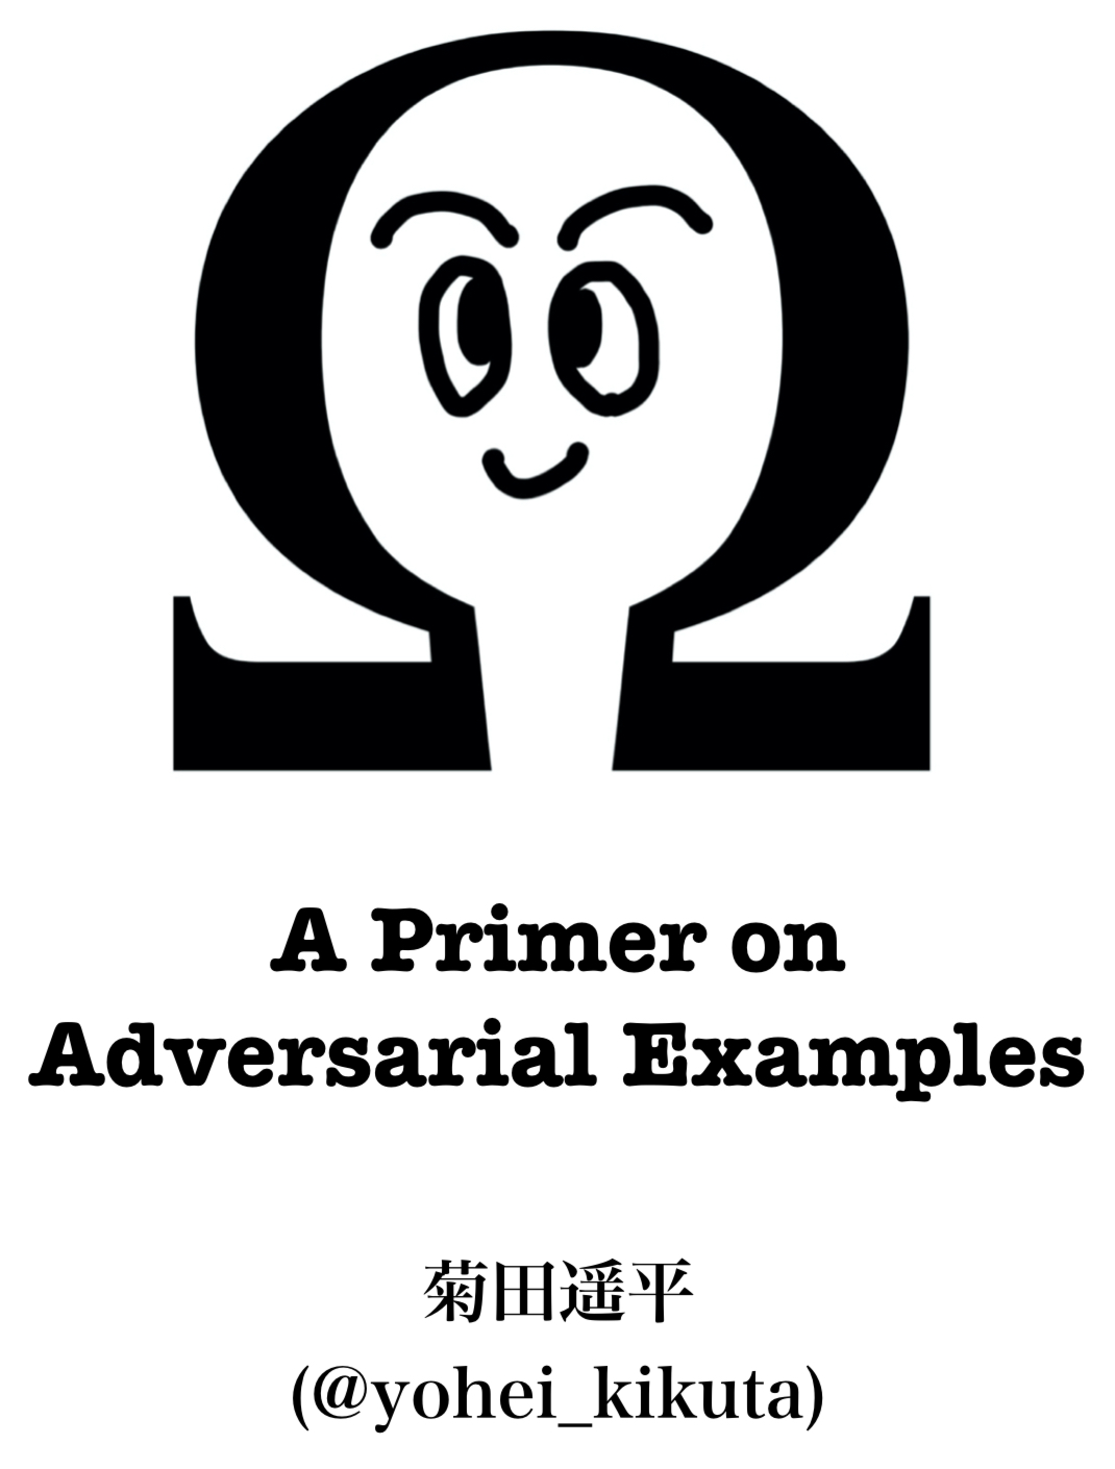
\includegraphics[width=15.5cm,height=22.0cm]{figures/cover.pdf}

\maketitle

\begin{abstract}
本書は, adversarial examples の基本的な内容と, adversarial examples を用いた攻撃手法とそれに対する防御手法に関してまとめたものである.
adversarial examples に関する様々なトピックを広く扱うというよりは, 独断と偏見でピックアップした攻撃手法と防御手法に注目し, それぞれの内容を表面的なレベルよりはもう少し踏み込んで理解することを目的としている.
この分野に明るくない人が読めば, adversarial examples の基本的な部分は理解して, そのあとの発展的な内容をフォローしている程度の基礎体力はつくのではないかと期待している.

adversarial examples そのものの性質やなぜ誤認識が生じるのかという原因などに関しては, 本書ではカバーしていない.
基礎体力がつけばそのような話題にもついていきやすいと思うので, 興味がある人はぜひ先に進んで欲しい.

本書では画像処理に対する adversarial examples のみを扱っており, 自然言語処理に対するものは扱っていない.
個人的には自然言語処理に対するものにも興味があって色々勉強したので自然言語処理の章も足したいのだが, 思ったよりページ数が多くなってしまったのと現状ではやる気が枯渇してしまった.
やる気が復活したらそのうち追記するかもしれない.

本書を読むのに要求される機械学習の知識は少ない.
勾配法の基礎を理解していて画像分析における classification と object detection モデルを触ったことがある人であれば, だいたいは理解できるのではないかと思う.
もう少し進んだ知識が要求される場合もあるが, 本書ではそういう場合には踏み込んで解説はしていないので, 必要があれば適宜読者の方で元論文を追うなりして補完して欲しい.

いくつかの攻撃手法や防御手法に関して PyTorch で実装したコードも \href{https://github.com/yoheikikuta/a-primar-on-adversarial-examples}{https://github.com/yoheikikuta/a-primar-on-adversarial-examples} で公開していて, 検証実験の結果も本書で解説している.

本書の TeX ファイルも公開していて, 本書の内容やコードに対する Pull Request は大歓迎なので, 改善点があればどしどし送って欲しい.
基本的に無料で公開しているが, 役に立ったという人は BOOTH で \href{https://yohei-kikuta.booth.pm/items/1867263}{https://yohei-kikuta.booth.pm/items/1867263} を買ってくれると著者にお金が入ります (内容は同じです).
\end{abstract}

\newpage
\tableofcontents
\newpage

%% To insert chapter title page.
% \newpage
% \vspace*{\stretch{1}}
% \begin{center}
% {\Huge 20180820 DAY 1}
% \end{center}
% \vspace*{\stretch{2}}
\clearpage
\section{導入と記号の定義}
\label{sec:introduction}
この章では adversarial examples がいかにして提案されたかという経緯と, 以降の章で必要となる記号やプログラム実行環境などの諸準備についてまとめる.



\subsection{導入}
\label{subsec:introduction}
adversarial examples は \cite{szegedy2013intriguing} によって初めて提案された.
これは人間には知覚しづらい摂動を入力データに加えて作成した新たな入力データのことを指し, 狭義\footnote{ここで狭義と言っているのは DNN 以外にも Support Vector Machine (SVM) や決定木や k Nearest Neighbor (kNN) に対する adversarial examples も考えられているためである \cite{papernot2016transferability}.この資料では DNN だけを対象にして, 他のモデルに対する adversarial examples は取り扱わない.}には Deep Neural Network (DNN) を誤認識させる性質を有するものである.
%
\begin{figure}[htbp]
\begin{center}
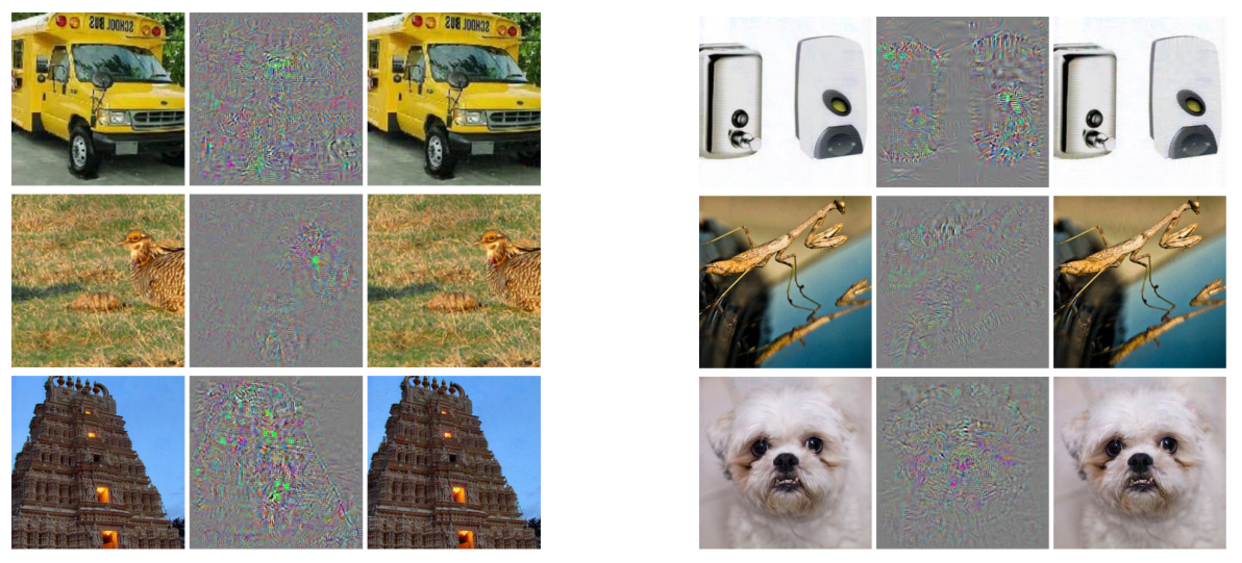
\includegraphics[width=12.0cm]{figures/szegedy-adv-examples.pdf}
\end{center}
\caption{adversarial examples の例.左列が元画像, 中央列が AlexNet \cite{krizhevsky2012imagenet} に対して生成された摂動, 右列が元画像に摂動を加えた画像である.
AlexNet は右列の画像に対して全て \textit{ostrich, Struthio camelus} (ダチョウ) と予測してしまう.図は \cite{szegedy2013intriguing} より引用.}
\label{fig:szegedy-adv-example}
\end{figure}
%

人間によるラベル予測や多くのカーネル法においては入力を少し変化\footnote{これは後に詳しく議論するが, あるノルムの意味で十分小さいと考えられる値で上から押さえられている摂動を入力に足すことを意味している.} させても出力には変化がなく (図 \ref{fig:szegedy-adv-example} の左列と右列は人間の目からは同じ対象物を表しているように見える), これを \cite{szegedy2013intriguing} では local generalization と呼んでる. このようなある種の「滑らかさ」は DNN においても成立するものと期待されていた.
しかし実際には図 \ref{fig:szegedy-adv-example} で示したように DNN においてはそのような期待が裏切られることが示された.
ある種の摂動が加えられた画像に対し, 人間の目には違いが見えづらいが, DNN は期待ところなる予測結果を返すという現象が発見されたのである.
その方法も誤認識させたいラベルに対する損失関数が小さくなるように準ニュートン法の Limited Broyden-Fletcher-Goldfarb-Shanno (L-BFGS) 法で摂動を見つけるというシンプルなものだったため, 多くの人々の興味を惹いた.

この論文の一年後に投稿された \cite{goodfellow2014explaining} ではよりシンプルな一階微分を用いた摂動を求める手法である Fast Gradient Sign Method (FGSM) が提案された.
これにより TensorFlow \cite{abadi2016tensorflow} を始めとする各種 DNN ライブラリでの扱いが容易になり, より多くの人にとって取り組みやすい対象となった.
研究が進むにつれて, adversarial examples は DNN の性質を探るという観点や実用上の脆弱性などの観点から大きく注目を集めるようになっていった.

DNN を用いたシステムやサービスを実際に運用するという立場から見ても, adversarial examples の存在は看過できないものである.
DNN はその予測性能の高さから様々なシステムに組み込まれるようになってきており, 顔認証や自動運転などはその代表例である.
自動運転のようにシステムのミスが人命に関わるような場合には品質保証は特に重要となるが, 映像から物体を認識するために DNN を使う場合は, adversarial examples による誤認識は実用に向けて大きな障壁となり得る.
同系統の議論として, DNN は予測の根拠が分かりづらいため説明可能性が必要だとする動きもあるが, adversarial examples は人間の期待と明白に異なる振る舞いを引き起こすものなので, より深刻であろう.

adversarial examples による攻撃は画像デジタルデータのピクセル値を直接変更する事に端を発したものであるが, その後の発展により物理的な環境下で対象物に摂動をプリントした紙やシールを貼る事で DNN を誤認識させることができるようになっているため, ここで述べている障壁は標語的なものではなく現実のものとなり得る.
悪意ある攻撃者が存在してもシステムを頑健に動作させるためにも, adversarial examples に関する理解を深めて適切に扱えるようになることは必要不可欠である.



\subsection{記号の定義}
\label{subsec:definition-symbols}
本書で使用する数学的な記号の定義を表 \ref{tb:notation} に列挙する.
入力データ $x$ に関しては height や width の次元を意識する必要性が生じる場面があまりないため, 必要なとき以外は単純に $\mathbb{R}^m$ の元として, 教師有りデータのラベルに関してはクラス数は $C$ とする.
本書では logit という言葉は softmax に入力する $C$ 次元のベクトルを指すものとする.
少し confusing な言葉遣いとして, logit というのは softmax に入力とするものを指す\footnote{
もともと logit 関数というのは sigmoid 関数の逆関数として定義されたものである: $\text{sigmoid} ( \text{logit}(p)) = p$.
これは任意の実数値を確率として解釈できる $[0, 1]$ に規格化するために sigmoid 関数がよく使われていたため, その逆関数に特別な名前を付与したことに由来する.
昨今では DNN が隆盛が甚だしく, DNN においては確率解釈のための規格化には softmax 関数が使われるため, logit という言葉が sotfmax 関数への入力を指すものとして使われることが増えてきた.
本書ではこの傾向に従い, softmax 関数への入力を logit と呼ぶことにする.
}.
モデルに関しては例えば $f_{\text{prob}} = \text{softmax} (f_{\text{logit}}(x))$ などの関係で結びつくものもあるが, 表記を簡潔にするため別個に定義している.
%
\begin{table}[htbp]
\begin{center}
\begin{tabular}{clccl}
\hline
表記  & 意味 & & 表記  & 意味 \\
\cline{1-2}
\cline{4-5}
$\mathcal{X}$ & 入力データ (画像) の集合 & & $x$ & $x \in \mathcal{X}$ なる要素で $x \in \mathbb{R}^m$ \\
& & & $x_{\text{adv}}$ & $x_{\text{adv}} = x + \omega$ なる adversarial example \\
$\mathcal{Y}$ & ラベルの集合 & & $y$ & $y \in \mathcal{Y}$ なる要素で $y \in \{1, 2, \dots, C\}$ \\
& & & $y_{\text{true}}$ & 入力データに対応する正しいラベル \\
& & & $y_{\text{atk-tgt}}$ & 摂動を加えることでモデルに誤認識させたいラベル \\
$\mathcal{D}_{\text{clean}}$ & 教師データの集合 & & $(x,y_{\text{true}})$ & 入力データとラベルの組からなる要素 \\
$\mathcal{D}_{\text{adv}}$ & adversarial データの集合 & & $(x_{\text{adv}},y)$ & 摂動を加えた入力データとラベルの組からなる要素 \\
$\Omega$ & 摂動の集合 & & $\omega$ & 入力データに加える摂動 ($x \rightarrow x + \omega$) で $\omega \in \mathbb{R}^m$ \\
& & & $\epsilon$ & 摂動の大きさをスカラー値で表現するもので $\epsilon \in \mathbb{R}_{+}$ \\
$\mathcal{F}$ & モデルの集合 & & & \\
& & & $f$ & 具体的な写像を考えずにモデルであることを示す \\
& & & $f_{\text{label}}$ & $f_{\text{label}}: x \rightarrow y$ なるモデル \\
& & & $f_{\text{prob}}$ & $x$ を入力として $C$ 次元のベクトルで確率を返す \\
& & & $f_{\text{logit}}$ & $x$ を入力として $C$ 次元のベクトルで logit を返す \\
& & & $f_{\text{bb}}$ & $x$ を入力として bounding box の情報を返す \\
$\mathcal{J}$ & loss function の集合 & & $J$ & $J: (f, x, y) \rightarrow v \in \mathbb{R}$ なる loss function  \\
& & & \\
& & & $\text{sign}$ & 符号関数 \\
& & & $\text{softmax}$ & softmax 関数: $p_i = \frac{\exp (f_{\text{logit}, i} (x))}{\sum_j \exp (f_{\text{logit}, j} (x))}$ \\
& & & $\text{softplus}$ & softplus 関数: $\ln (1 + \exp (x))$ \\
\hline
\end{tabular}
\caption{本書で使用する記号の定義. \label{tb:notation}}
\end{center}
\end{table}
%



\subsection{略語の定義}
\label{subsec:definition-abbreviations}
本書で使用する略語の定義を表 \ref{tb:abbreviation} に列挙する.
以降に出てくる略語は完全な表記を併記しないため, この表 \ref{tb:abbreviation} を参照すること.
例えば VGG は研究グループ名が特定のモデルを指す意味で使われるようになったもので, 略語だけ見ても何を指しているか分からないものも多いが, 慣例であるので致し方ない.
%
\begin{table}[htbp]
\begin{center}
\begin{tabular}{c|c}
\hline
略語 & 完全な表記 \\
\hline
bbox & bounding box \\
CIFAR & Canadian Institute For Advanced Research \\
CNN & Convolutional Neural Network \\
CW & Carlini-Wagner \\
DNN & Deep Neural Network \\
ELU & Exponential Linear Unit \\
Faster-RCNN & Faster-Regions with CNN features \\
FCN & Fully Convolutional Network \\
FGSM & Fast Gradient Sign Method \\
GAN & Generative Adversarial Network \\
ILSVRC & ImageNet Large Scale Visual Recognition Challenge \\
IoU & Intersection of Union \\
I+FGSM & Iterative Fast Gradient Sign Method \\
kNN & k Nearest Neighbor \\
L-BFGS & Limited Broyden-Fletcher-Goldfarb-Shanno \\
mAP & mean Average Precision \\
mIoU & mean IoU \\
MI+FGSM & Momentum Iterative Fast Gradient Sign Method \\
MLP & Multi-Layer Perceptron \\
MNIST & Modified National Institute of Standards and Technology \\
MSCOCO & Microsoft Common Objects in Context \\
NIN & Network In Network \\
NMS & Non Maximum Supression \\
R+FGSM & Randomized Fast Gradient Sign Method \\
PascalVOC & PASCAL Visual Object Classes \\
PGD & Projected Gradient Descent \\
RBF & Radial Basis Function \\
ReLU & Rectified Linear Unit \\
RPN & Region Proposal Network \\
SSIM & Structural SIMilarity \\
SVHN & Street View House Numbers \\
VGG & Visual Geometry Group \\
WGAN & Wasserstein GAN \\
ZF & Zeiler-Fergus\\
\hline
\end{tabular}
\caption{
本書で使用する略語の定義.
alphabetical に並べている.
\label{tb:abbreviation}
}
\end{center}
\end{table}
%



\subsection{検証プログラムに関する注意事項}
\label{subsec:note_on_code}
本書で使用するプログラムは GitHub レポジトリ \href{https://github.com/yoheikikuta/a-primer-on-adversarial-examples}{https://github.com/yoheikikuta/a-primer-on-adversarial-examples} で管理されている.
環境構築手順などは README.md に記載しているのでそちらを参照のこと.
基本的には docker \href{https://www.docker.com/}{https://www.docker.com/} を利用して Anaconda \href{https://www.anaconda.com/}{https://www.anaconda.com/} 環境を構築し, その上で PyTorch \cite{paszke2019pytorch} を使って実装をしている.
docker のインストール方法は公式ページ \href{https://docs.docker.com/install}{https://docs.docker.com/install} を参照のこと.
docker 環境が構築されていれば, git clone したレポジトリの top directory で下記コマンドを実行することで image の build と container の作成を実施できる.
%
\begin{lstlisting}[language=bash]
  $ docker build -t work -f Dockerfile .
  $ docker run --rm -it -v $PWD:/work work
  (do something in the container)
\end{lstlisting}
%

実行環境は基本的にローカルの PC で CPU を使用することを想定しているが, 計算負荷の大きい場面では \href{https://colab.research.google.com}{https://colab.research.google.com} の GPU 環境\footnote{
20200206 現在, Colaboratory では一回に最長 12 時間まで GPU/TPU を無料で使用できる.
notebook は放置していると仮想マシンから切断されて計算が止まってしまうため, 再接続を促されたらブラウザを操作して再接続をしたり, 定期的に notebook を開いているタブをリロードしたり, という必要がある.
この切断の時間間隔は以前は 90 分という話を聞くことが多かったが, 体感ではこの時間間隔は一定時間ではないようにも感じる (詳しく計測はしていない).
また, GPU は K80, T4, P4, P100 がランダムに割り当てられるとのことだが, 個人的には T4 か P100 のことが多い.
同じコードを実行しても割り当てられた GPU によって計算時間が変わってくるので注意が必要である.
詳しくは公式ページ \href{https://research.google.com/colaboratory/faq.html}{https://research.google.com/colaboratory/faq.html} を参照のこと.
有料だがより長時間使用したり良い GPU を優先的に使用できる Colab Pro も発表されているが, 20200206 時点では米国でのみ利用可能である.
}を使用している.
その際に使用した notebook ファイルも同梱している.
\clearpage
\section{Adversarial Examples の定式化}
\label{sec:formulation}



\subsection{Adversarial Examples の形式的な定義}
\label{subsec:def-adv-examples}
教師あり分類問題 $f_{\text{label}}: x \rightarrow y$ を考え, モデルによる予測が $f(x) = y_{\text{true}}$ となるようなデータの組 $(x, y_{\text{true}})$ を考える\footnote{
adversarial examples は, 元々モデルの予測が正しいような入力データに摂動を加えて正しかった予測を間違えさせることを目的としているので, 出発点としてモデルによる予測が正しい予測になっている入力データのみを対象にするという意味でこのように書いている.
ただし, 実際の実験では元の予測が合っていても合っていなくてもより間違えさせるような摂動を加えて評価することも多いため, ここでの取り扱いは adversarial examples を分かりやすく定義するためのものである.
}.
adversarial examples とは, 入力 $x$ に摂動 $\omega$ を加えることによって, もともとは正しかったモデルの予測を間違ったものに変えるような入力データ $x_{\text{adv}}$ である.
%
\begin{eqnarray}
f(x + \omega) = f(x_{\text{adv}}) \neq y_{\text{true}} \ \ \text{with some constraint on} \ \omega.
\label{eq:def-adv-examples}
\end{eqnarray}
%

摂動を特徴づけるために何かしらの制限を $\omega$ に課しており, この制限は人間の目にとっては $x_{\text{adv}}$ が $y_{true}$ を正解ラベルに持つのが自然であると考えられるように付与する\footnote{
adversarial examples の大きなモチベーションの一つは, 人間の目にはある正解ラベルを持つように見える入力データが DNN モデルには異なるラベルであると予測されるデータを作成することであり, そこから DNN モデルの特徴の理解や人間との認識の理解などを深めることが期待されている.
研究によっては DNN モデルも人間も間違えるような adversarial examples を考えている \cite{elsayed2018adversarial} などもあるが, 本書ではこのような内容には踏み込まない.
}.
よく使われる制限としては $\omega$ の $l_2$ ノルムや $l_\infty$ ノルムが一定値を超えないようにするというものが挙げられる.
これらは数学的・プログラム的に扱いやすいというのが主たる理由で深淵な理由があるわけではない.
一方で, 制限として「人間の目にとって落書きに見えるような」という定量化し難いものを課す場合もあるため, 式 \ref{eq:def-adv-examples} での定式化はかなり抽象的なものとしている.
より細かい分類や具体的な手法を解説する際に, 具体的にどのような制限が課されるかを明示する.

摂動となる $\omega$ をどのように求めるかが adversarial examples を作成するための主たる要素の一つであり, のちに具体的な手法を解説する際に紹介していく.
ここでは, 最も簡単な FGSM による摂動の構成方法を例示しておく.
$\omega$ を $x$ と同じ次元を持つ摂動, $\epsilon \in \mathbb{R}$ を $x$ の各要素が取りうる値の範囲の大きさと比べて十分小さいスカラー, $J(f, x, y)$ を loss function としたとき, 以下のように loss の一階微分を用いて $x_{\text{adv}}$ を求めるのが FGSM である.
%
\begin{eqnarray}
x_{\text{adv}} = x + \omega = x + \epsilon \cdot \text{sign} ( \nabla_x J (f, x, y_{\text{true}}) ).
\label{eq:adv-fgsm}
\end{eqnarray}
%
DNN の学習で通常実施するようなパラメタの微分ではなく, データの微分 $\nabla_x$ であることに注意されたい.
これは, adversarial examples の作成においては更新するのはモデルのパラメタではなくて入力データとなるためである.
この微分で入力データと同じ $m$ 次元のベクトルが得られ, その符号を取っているので, 各要素において一階微分の意味で loss function が増大する方向を取得している\footnote{
モデル学習のためによく使うパラメタの更新は $\eta > 0$ を用いて $\theta_{\text{updated}} = \theta - \eta \nabla_\theta J$ というものだったことを思い出すと, 第二項の符号が逆であり, パラメタの更新の場合は loss を小さくする方向に, adversarial examples の場合は loss を大きくする方向に動かしていることが理解できる.
FGSM に関しては \ref{subsec:fgsm-based} 節で改めて解説する.
}.
あとは摂動の大きさを調節するために $\epsilon$ を乗じているだけで, シンプルな構成方法となっていることが理解できる.

データが 2 次元の簡単な場合で図示したのが図 \ref{fig:fgsm-loss} である.
あるデータ $x$ における微分 $\nabla_x J$ を計算し, その $\text{sign}$ を取ることで $x_1, x_2$ 成分それぞれに対して正負どちらの方向に動かせば loss が大きくなるかということが分かる (図の場合はどちらも正の方向).
あとはそれに $\epsilon$ という単一の微少量を掛けて $x$ に足すことで loss が大きくなるような $x_{\text{adv}}$ を構築している.
この例では 2 次元であるので $\epsilon$ が小さいため loss の増大分は大したことはないが, これが 10,000 次元など大きくなってくると小さな $\epsilon$ が積み重なって大きな loss の増大に繋がり, その結果モデルの logit は clean なデータの場合とはかけ離れたものになり, $y_{\text{true}}$ とは異なるラベルと予測するようになる.
%
\begin{figure}[htbp]
\begin{center}
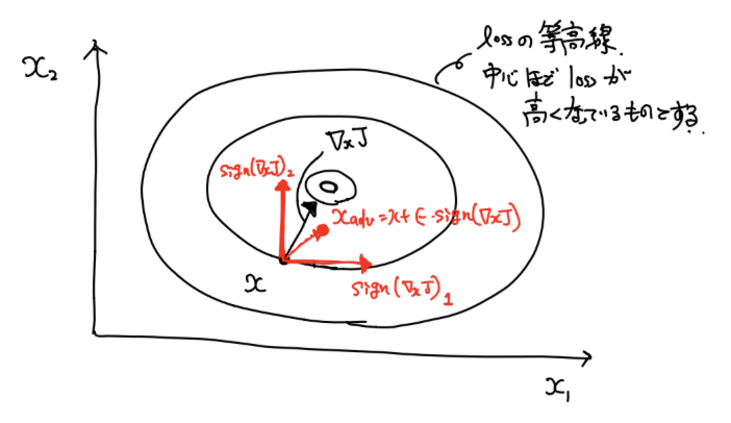
\includegraphics[width=12.0cm]{figures/fgsm-loss.pdf}
\end{center}
\caption{
FGSM による adversarial examples 作成のイメージ図.
データが 2 次元 $(x_1, x_2)$ の場合で, 黒い等高線が loss の等高線を表していて, 中心ほど loss が高くなっているものとする.
あるデータ $x$ における微分とそれに基づいて $x_{\text{adv}}$ を作る様子を示している.
}
\label{fig:fgsm-loss}
\end{figure}
%



\subsection{Adversarial Examples を用いた攻撃とそれに対する防御}
\label{subsec:attack-and-defense}
前節で定義した adversarial examples を用いて, DNN による分類をサブシステムとして含むシステムに攻撃が可能となる.
ここで言う攻撃とは, 攻撃者が adversarial examples を用いて DNN モデルの予測を誤った予測に変えることで, システムの利用者が不利益を被るものである.

具体的な例として自動運転システムのサブシステムとして車載搭載カメラで標識を画像認識する場合を考える.
システムが adversarial examples を用いた攻撃を受けた場合\footnote{
前節で紹介した FGSM は攻撃対象のモデルの微分を必要とするもので, モデルの微分情報が取得できないケースでは使用できないものである.
しかし, のちに紹介するように adversarial examples を構築する際には必ずしもモデルの情報は取得できる必要はないため, このような攻撃は現実に生じ得るものである.
}, 一旦停止の標識がある場所で一旦停止の標識と認識して止まるべき状況で速度制限の標識と誤認識することで止まらずに進んでしまい, 大事故に繋がる可能性がある.
画像認識モデルの大きな応用の一つが自動運転における人や標識などの物体認識であり, モデルの誤認識が引き起こす影響も大きいため, adversarial examples の研究でもよく題材となる.
現時点での研究でも, adversarial examples となり得る標識を実際に設置し\footnote{どのようにこれを実現するかはのちに具体的な例で紹介するが, 標識に摂動をプリントしたシールを貼ったりすることで adversarial examples を作成することが可能である.}, 車載カメラで撮影した画像がモデルに誤認識を引き起こすかを調べたりするところまで来ているため, 近い将来に実用面でも重要となる可能性を十分に秘めている.

別の例として顔認識システムのサブシステムとしてカメラで人物を特定する場合を考える.
顔認識で人物を特定して支払情報と紐づけて物品購入の支払いをする場合, adversarial examples を用いた攻撃によって実際に物品を購入した人物とは別の人物が支払いを要求される可能性がある.
また, 人物検出を実施するモデルに対して攻撃を加えて人間がいないと誤認識させることで, システムには人間が存在することを悟られることなく行動することができるかもしれない.

ここで挙げた例は極端に単純化した場合で実際のシステムはもっと頑健に作られているべきであるが, DNN に対する adversarial examples 自体は DNN 以外のシステムの頑健性とは独立に厳然として存在するものであり, 品質が保証されているべきシステムを実運用する際には脅威となり得るものである.

このような攻撃が存在する以上, 如何にして防御をしてシステムを頑健にするかが重要になる.
防御方法として, 摂動が加えられた入力データ $x_{\text{adv}}$ に対しても正しいラベル $y_{\text{true}}$ を返すようなモデルを構築する方法と,  $x_{\text{adv}}$ が adversarial examples であることを検出\footnote{
本来のモデルの予測とは別に何かしらの機構で入力データが正常なデータか adversarial examples かを二値分類する.
}してそれをシステム利用者に知らせる方法と, のようにこれらのアプローチを別の手法と分類する文献もあるが, 本書ではこれらを細かく分けずに防御方法という一つの枠内で取り扱うものとする.

攻撃側は adversarial examples による攻撃だけを考えればよく, adversarial examples の作成に多大なコスト (人的コストや時間的コストや計算資源的コスト)が掛かったとしても一度でも成功すれば被攻撃者に大きな損害を与え得る.
一方で防御側はそもそものモデルの予測が本来使いたいものなので, adversarial examples に対してはあまりコストを掛けずに対応したいというモチベーションがある.
adversarial examples に対する防御性能は高くても, モデル設計を一からやり直す必要があったり, 推論の速度が何倍にもなってしまったりするのはコストが高すぎるという状況も多いだろう.
また, 本来の目的である予測が degradation\footnote{ここでは adversarial examples に対応するようにモデルをアップデートしたときに, clean なデータに対するモデルの予測精度が低下することを指す.} を起こしてしまうのも避けたい.
さらに, 防御側は攻撃側の手法のアップデートに対応してシステムを逐次改善してアップデートしていく必要もあるため, コストの観点は重要となる.
現状の研究ではこの観点はそれほど重視されていないよう見受けられるが間違いなく重要であり, 本書では最初の一歩として定性的なコストの評価を試みている.

重要なことは, 攻撃と防御は表裏一体であり, どんなモデルに対してもうまくいく攻撃やその逆のどんな adversarial examples に対してもうまく防御できる手法は存在しないということである.
攻撃も防御も様々な手法が提案されており, それは今後も続くものであるため, 常に新しい手法を理解して取り入れていく必要がある.

次節以降では 2019 年末時点での攻撃と防御のそれぞれの典型的な手法を概念的に分類して整理し, 次章以降でそれらの詳細を解説していく.



\subsection{Adversarial Examples を用いた攻撃の分類}
\label{subsec:classification-attack}
モデルを誤認識させるための adversarial examples を作成する際の作成方法を分類する.
\cite{yuan2019adversarial} や \cite{wiyatno2019adversarial} のような adversarial examples に関するレビュー論文においても様々な軸で分類がなされているが, 統一的な分類方法は定まっていないように思われる.
本書では, 先行研究を踏まえつつ, 著者が特に重要と考える以下の観点を用いて手法を分類する.
A $\lor$ B の項目は対象の攻撃手法が A か B のどちらかに分類されることを意味している.
%
\begin{itemize}
  \item Digital (Pixel) attack $\lor$ Physical attack\\
  前者は画像のピクセルデータを直接変更して攻撃するもので, 後者は電子データではなく物理的環境で撮影する場合に対象物に物理的変更を加えて攻撃する.
  digital attack はモデルの性能を深く理解するために重要であり, また画像認識 API への攻撃などにも用いられる.
  physical attack は自動運転など物理的環境で稼働するシステムへの攻撃に用いられる.
  \item Classifier $\lor$ Detector\\
  前者は入力データに対してラベルを返すもので, 後者は入力データに対して複数の bbox の位置情報と各 bbox に対するクラス予測を返すものとする.
  adversarial examples の研究は classifier を対象とするものが多いが, 実運用では detector にも有効であるかの観点も重要であり, detector を対象とする研究も増えてきている.
  \item 摂動作成時に使用するデータ\\
  adversarial examples を作成する際にどのようなデータを使用するかという観点.
  単純なものとしては攻撃対象データを用いてそこに摂動を加えるというものが挙げられるが, モデルの構造だけに注目してデータを必要としない手法や, renderer を介する手法で 3D object データを用いるものなど多様な発展がある.
  \item 画像全体への摂動 $\lor$ 対象物のみへの摂動\\
  前者は画像の任意の点でのピクセル値を変えるもので, 後者は例えばある標識を誤認識させたい場合に対象物である標識のみに摂動を付与するものである.
  基本的に前者が digital attack で後者が physical attack である\footnote{
  もし入力データが時間不変なものであれば画像全体を対象として摂動を構築した方が攻撃成功率が高まるが, physical attack では時事刻々とシステムへ入力される画像が変わるため, 対象物以外に摂動を加えても距離や角度の変化によって誤認識を引き起こすことのできないものとなりがちである.
  physical attack では対象物のみに摂動を加え, その摂動を含む対象物がどのように撮影されようとも誤認識させるようにする必要がある.
  }
  が, digital attack でも対象物のみに摂動を付与する工夫をしてその後の physical attack につなげようとする手法も存在する.
  \item 知覚しづらさの定義\\
  作成した adversarial examples がどのような意味で「摂動」になっているかという観点.
  単純なものとしては摂動の $l_2$ ノルムが上から押さえられているというような定量的な指標が用いられ, これは元画像からの差分の評価に使えるしこの指標が小さいほど人間の目にとっても元画像と区別がつきにくい.
  発展的な指標として, 落書きのように見える (ので人間にとって特殊なノイズだと気付きにくい) という定量化が難しいものや色味が変わるだけ (なのでピクセル値の意味では変化が大きくても人間にとっては特殊なノイズだと気付きにくい) というもの, などもある.
  \item White box $\lor$ Black box\\
  前者はモデルの情報 (アーキテクチャや loss やその微分) を使ってモデルの誤認識率を高めるための手法である.
  後者はモデルの入出力のみにアクセスできる.
  実際の攻撃では black box の場合がほとんどであるが, white box は最悪ケースの想定やモデルの構造の理解, black box attack を構築するための材料として使用するなどの用途がある.
  なお, 真の black box とは出力として出力されたラベルのみを使用できるものであるべきだが, 現状は多くの提案手法で出力の全クラスに対応する softmax 値を使用している\footnote{
  $C$ クラス分類問題において, $C$ 次元の softmax 値を全て使用しているという意味.
  例えば商用の画像認識 API などは確率値の高い上位 $N (< C)$ 件のラベルしか返さないものが多く, このような設定は非現実的である.
  真の black box attack を実現している手法として \cite{tsuzuku2019structural} などが挙げられる.
  }.
\end{itemize}
%

ここで取り上げていないが典型的な観点として, Targeted / Non-targeted という, 特定のラベルに誤認識させるか正解のラベル以外なら何でもよいかというものがある.
これは前述のような真の black box attack では non-targeted しか選べないことと, targeted の多くの手法は non-targeted として使うこともできるという理由から除外している.

ここまで挙げたのは個別の手法の分類のための観点だが, 実運用上では攻撃者がどの情報にアクセスできるかが重要な観点である.
例えば画像認識 API への攻撃ならば digital attack となり, 自動運転システムの画像認識サブシステムへの攻撃ならば physical attack となる.
攻撃側としては現実的には black box attack を採用するしかないが, 防御側としてはモデルの振る舞いを理解しておくためにも white box attack を把握しておくことは不可欠である.
実運用上の観点から攻撃方法を分類したものが以下の図 \ref{fig:attack-summary} である.
例で挙げているのは \href{https://arxiv.org}{https://arxiv.org} の論文であり, 数字は arXiv の投稿番号である.
投稿番号は [YYMM.xxxxx] という形式で与えられており, 出版年の下 2 桁と月が最初の 4 文字で, 以降の数字は出版順に振られるようになっている.
本書では対象とする論文が arXiv にある場合はそれを参照するようにし, 投稿番号を併せて記載するようにする.
%
\begin{figure}[htbp]
\begin{center}
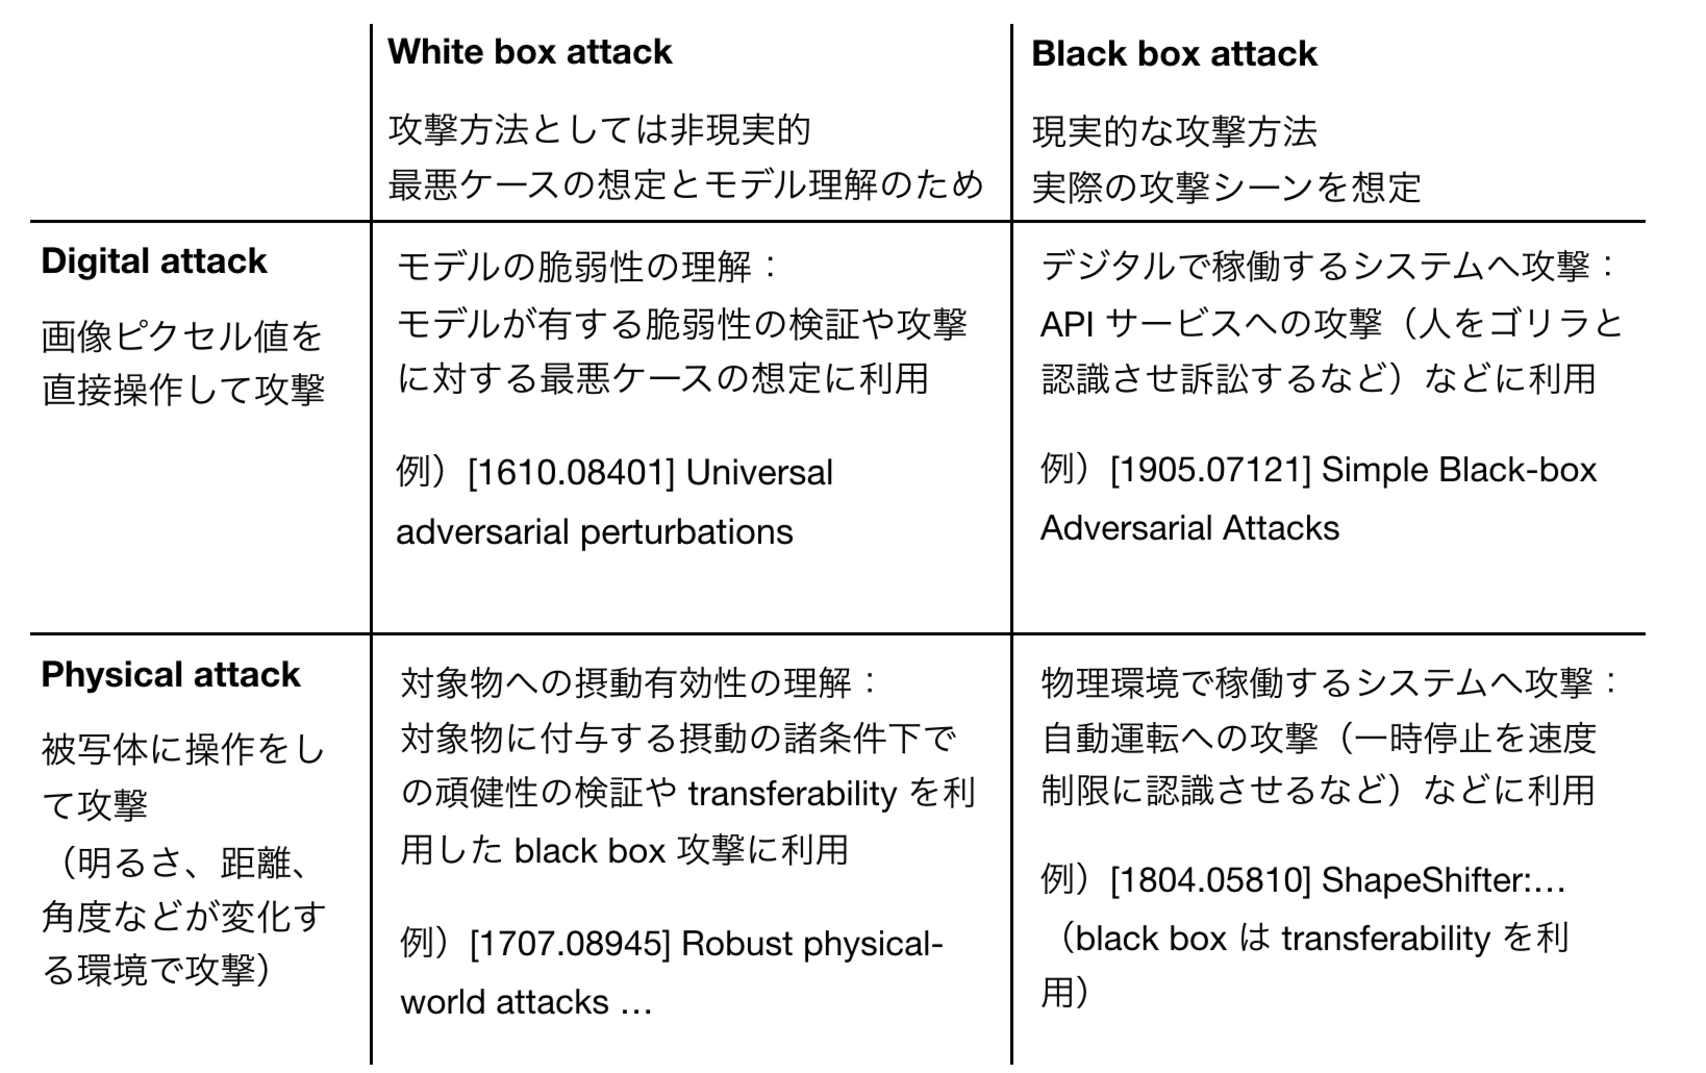
\includegraphics[width=15.0cm]{figures/attack-summary.pdf}
\end{center}
\caption{実運用上の観点に基づく攻撃方法の分類. 例は arXiv の論文であり, 投稿番号とタイトル (の一部) を記載している.}
\label{fig:attack-summary}
\end{figure}
%



\subsection{Adversarial Examples に対する防御の分類}
\label{subsec:classification-defense}
adversarial examples に対する防御手法を分類する.
攻撃方法と同様に著者が重要と考える観点で分類をするが, 他ではあまり見られない独自の観点が多いことに注意されたい.
本書の特徴として, 研究ではあまり取り上げられないが実運用上問題となる観点である「当該手法を導入するための対応コスト」という観点を含めている.
%
\begin{itemize}
  \item 基本戦略\\
  防御のための大まかな戦略を次の 4 つから成るものとした: 正則化 (学習時の loss function に正則化項を加える), 入力データ変更 (予測対象となる入力データを加工する), 予測モデル変更 (本来の予測モデルのアーキテクチャに手を加える), 外部モデル使用 (予測モデル以外のモデルを使用する).\\
  これらの分類を防御方法の分類とすることが多いと思われるが, 本書ではコストの観点を重視して分類の観点として取り入れているので, ある程度粒度を合わせるためにこれらの細かい分類をまとめて基本戦略として一つの観点にしている.
  \item 使用する外部リソース\\
  予測モデルの構築には予測モデルのアーキテクチャと学習データを準備すればよいが, 防御手法によっては更なるリソースを必要とするものも多い.
  予測モデルとは別のモデルや外部のデータ, そして防御手法のための adversarial examples\footnote{
  これは予測モデルと学習データがあれば作成できるものであるが, 便宜上外部リソースとして扱うことにする.
  } などが対象となる外部リソースである.
  \item 対応コスト (人的コスト, 推論コスト)\\
  当該の防御手法を導入するためにどれくらいのコストを必要とするかという観点.
  ここでは 2 種類のコストを考えおり, 人的コストはリソースの準備やコーディングの量や学習の待ち時間を想定しており, 推論コストは予測時に本来の予測モデルによる予測と比べて余分に必要となる計算量を想定している.
  実運用上重要だが定量化が難しい観点であるため, 大・中・小の大まかな 3 段階で評価する. 
\end{itemize}
%

繰り返しとなるが, 防御方法において重要なのはその方法を導入する際のコストがどの程度で, 実運用のプロセスに組み込むことが可能なのか, という点である.
この点を明確にすべく, モデル設計から予測までのプロセスを分解し, 防御方法がプロセスのどの段階にマッピングされるかをまとめたものが以下の図 \ref{fig:defense-process} である.
%
\begin{figure}[htbp]
\begin{center}
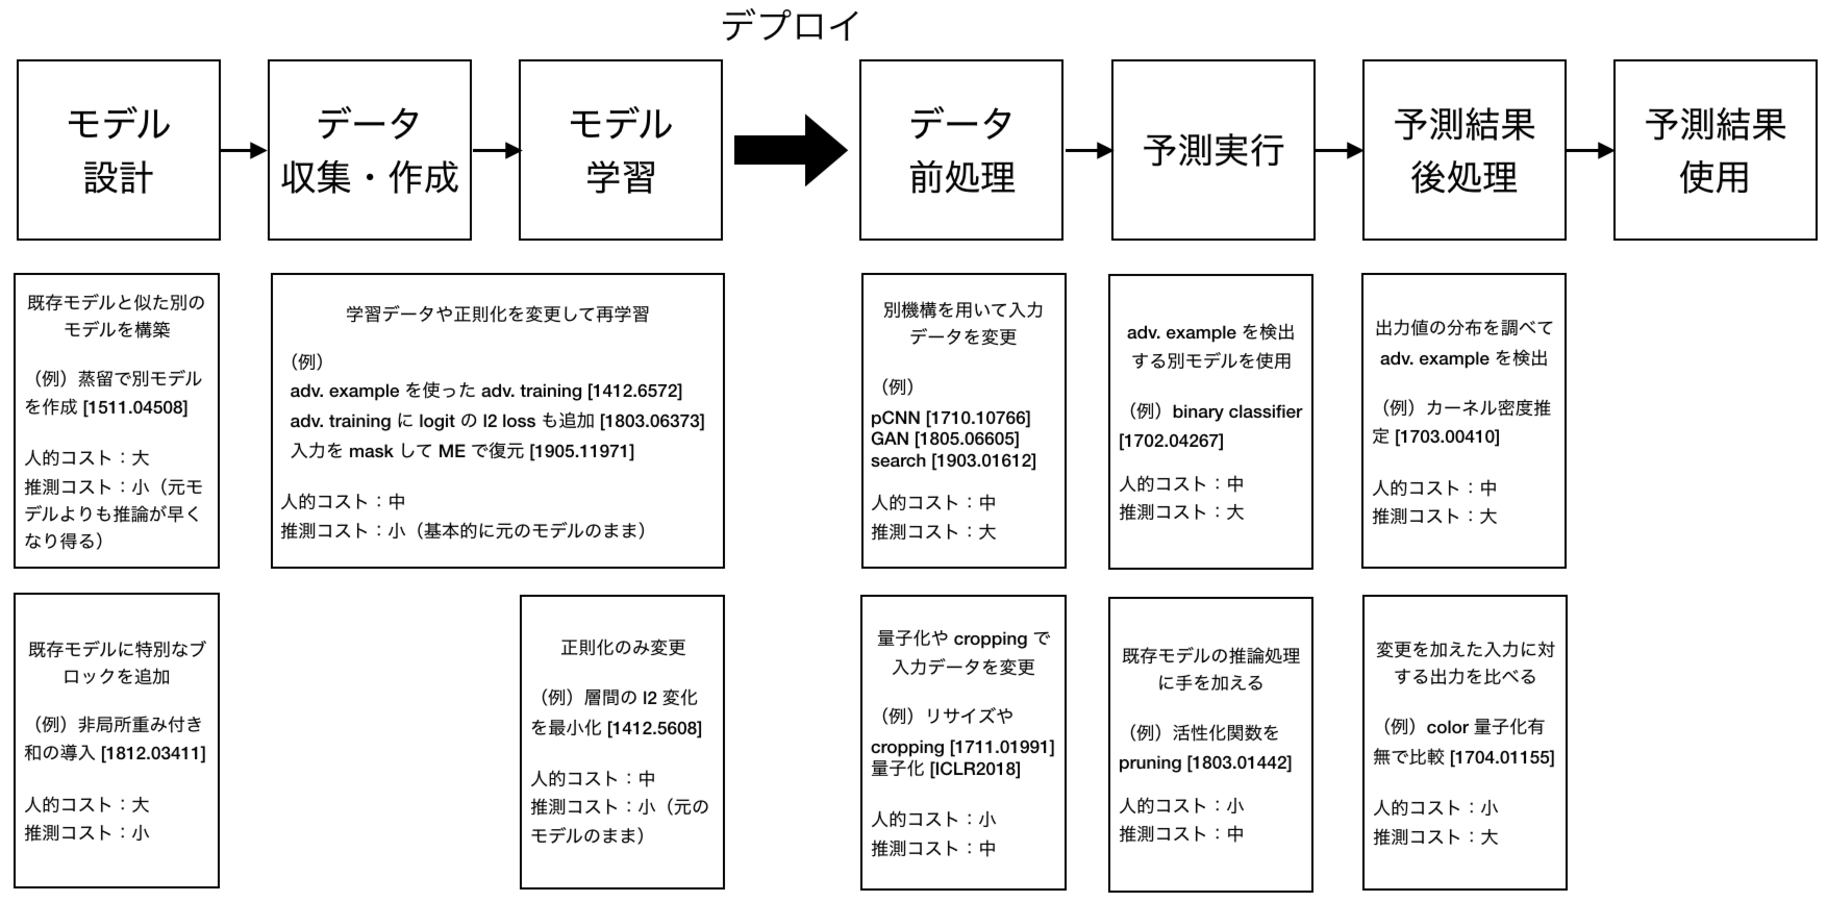
\includegraphics[width=16.0cm]{figures/defense-process.pdf}
\end{center}
\caption{
防御方法のプロセスへのマッピング.
それぞれの枠が同じ種類の防御方法を表しており, 簡単な説明と具体的な論文の例, 対応コストを記載している.
このコストは該当する枠の大まかな目安に過ぎず, 個別の手法毎に差があるため詳しくは個別の手法を見るように注意されたい.
文字が小さいため拡大して見ることを推奨.
}
\label{fig:defense-process}
\end{figure}
%
\clearpage
\section{Adversarial Examples の実験方法と典型的なデータセットの解説}
\label{sec:exp-design-and-data}
この章では、adversarial examples の実験として用いられる典型的な手順を解説すると共に, 実験でよく使われるデータセットを解説する.



\subsection{Adversarial Examples の実験方法}
\label{subsec:exp-design}
adversarial examples を使った実験は大別すると以下の 3 つの目的から成る.
%
\begin{itemize}
  \item 攻撃目的\\
  モデルの正答率を下げるために adversarial examples を使う.
  攻撃はモデルの正答率を低くするほど、効率的(計算量が少ない、adversarial examples を作成するために必要なシステムへのクエリ回数が少ない、など)であるほど良い攻撃であると解釈される.
  モデルの正答率を表記する場合とモデルの誤認識率(1 - 正答率)を表記する場合がある.
  \item 防御目的\\
  モデル学習時に adversarial examples を使うことで, 攻撃に対して耐性を高める.
  防御はモデルの正答率を高めるほど良い防御であると解釈され, この観点だけを議論している研究が多い.
  実運用を考えれば防御方法は効率的(導入の人的・計算資源的コストが少ない、推論時の速度に対する影響が少ない、など)であるほど好ましいが, このような観点を議論している研究はまだあまり見かけない.
  \item データやモデルを理解する目的\\
  adversarial examples はモデルに対する特殊なバグのようなものでなくデータに内在する特徴である \cite{ilyas2019adversarial} と捉えたり, adversarial examples を使って overfitting を検出する \cite{werpachowski2019detecting} など, データやモデルの特徴を理解するために adversarial examples を使う.
  これらは adversarial examples の活用として興味深い方向性ではあるが, 本書では扱わない.
\end{itemize}
%

攻撃目的の実験はシンプルだが, 防御目的の実験は注意が必要である.
登場するデータを整理しながら典型的な防御目的の実験手順を見ていく.

データの集合としては元々の教師データの集合 $\mathcal{D}_{\text{clean}}$ があり, これは train/test を含んでいる.
少し冗長ではあるが, ここでの説明に限りそれらを $\mathcal{D}_{\text{clean, train}}, \mathcal{D}_{\text{clean, test}}$ と表記する.

防御方法で adversarial examples を使う場合には, train に対応する $\mathcal{D}_{\text{adv, train}}$ を作成し学習に利用する\footnote{
これを使わずに防御する手法も数多く提案されているため, 必ず使うわけではない
}.
テスト時には, 学習したモデルを攻撃するための $\mathcal{D}_{\text{adv, test}}$ を作成し, これに対する正答率を測ることで防御方法の性能を議論する.

この手順のみに注目している研究も少なくないが, 実際には防御方法を入れたことによって $\mathcal{D}_{\text{clean, test}}$ に対する影響が生じ得るため, このデータに対する正答率も合わせて評価するのがより正しい手順となる.

本書では画像データのみに着目するためこのような説明となっているが, 自然言語処理では学習時に adversarial examples を利用するのは防御のためというより $\mathcal{D}_{\text{clean, test}}$ に対する正答率を高めるためという目的で使われることが多い\footnote{
もちろん画像データでもそのような目的で adversarial examples を使っているものがあり, 例えば \cite{xie2019adversarial} などが挙げられる.
}.
このような背景もあり, adversarial examples を用いた学習で汎化性能を向上させる, というような言及がある場合は $\mathcal{D}_{\text{clean, test}}$ に対するものか $\mathcal{D}_{\text{adv, test}}$ に対するものかを文脈から判断する必要がある.
本書における防御方法の実験では, 必ず両方のデータで正答率を評価するようにしている.



\subsection{Adversarial Examples の実験でよく使われるデータセット}
\label{subsec:typical-dataset}
adversarial examples の実験でよく用いられるデータセットを紹介する.
部外者がアクセスできない論文独自のデータセットは取り上げず, オープンアクセスのデータセットのみを対象とする.

train/test の画像枚数, 画像サイズ [channel, height, width], クラス数, 簡単な特徴をデータセット毎に記載する.
%
\begin{itemize}
  \item MNIST \href{http://yann.lecun.com/exdb/mnist/}{http://yann.lecun.com/exdb/mnist/}\\
  train/test : 60,000/10,000\\
  画像サイズ : [1, 28, 28]\\
  クラス数 : 10\\
  特徴 : 手書き数字文字 (0 から 9 まで) のデータセット.
  \item fashion MNIST \href{https://github.com/zalandoresearch/fashion-mnist}{https://github.com/zalandoresearch/fashion-mnist}\\
  train/test : 60,000/10,000\\
  画像サイズ : [1, 28, 28]\\
  クラス数 : 10\\
  特徴 : MNIST のファッション画像版のデータセット. クラスは T シャツやズボンなど.
  \item CIFAR10 \href{https://www.cs.toronto.edu/~kriz/cifar.html}{https://www.cs.toronto.edu/~kriz/cifar.html}\\
  train/test : 50,000/10,000\\
  画像サイズ : [3, 32, 32]\\
  クラス数 : 10\\
  特徴 : 飛行機や車などの互いに overlap がない排他的なクラスのデータセット.
  \item CIFAR100 \href{https://www.cs.toronto.edu/~kriz/cifar.html}{https://www.cs.toronto.edu/~kriz/cifar.html}\\
  train/test : 50,000/10,000\\
  画像サイズ : [3, 32, 32]\\
  クラス数 : 100\\
  特徴 : CIFAR10 のクラス数を増やして 1 クラス毎の画像枚数を減らしたデータセット.
  \item SVHN \href{http://ufldl.stanford.edu/housenumbers}{http://ufldl.stanford.edu/housenumbers}\\
  train/test : 73,257/26,032 (追加学習用の 531,131 件のデータもある)\\
  画像サイズ : [3, 32, 32]\\
  クラス数 : 10\\
  特徴 : Google Street View Image から取得した数字画像のデータセット. 実験でよく使われるのは一枚の画像に一つの数字が写るように 32 * 32 に切り出した画像(実際には一枚の画像に複数の数字が写り込むものも多い)だが, 切り出す前の解像度がバラバラの元データも提供されている.
  \item GTSRB \href{https://www.sciencedirect.com/science/article/abs/pii/S0893608012000457?via\%3Dihub}{https://www.sciencedirect.com/science/article/abs/pii/S0893608012000457?via\%3Dihub}\\
  train/test : 39,209/12,630\\
  画像サイズ : カラー画像で height と width はバラバラで, それぞれ平均は 50 程度.\\
  クラス数 : 43\\
  特徴 : ドイツの標識のデータセット. 標識部分を切り出し, 標識の種類が分類クラスになっている.
  \item ILSVRC \href{http://www.image-net.org/challenges/LSVRC/}{http://www.image-net.org/challenges/LSVRC/}\\
  train/valid : 1,281,167/50,000 (\href{https://www.tensorflow.org/datasets/catalog/imagenet2012}{https://www.tensorflow.org/datasets/catalog/imagenet2012})\\
  画像サイズ : カラー画像で height と width はバラバラで, 平均は (450, 400) 程度.\\
  クラス数 : 1,000\\
  特徴 : 画像分析のコンペティションで用いられる大規模データセット. 年によってデータに変更が加えられるが, classification は 2012 から変わらないので ILSVRC2012 のデータと表記して使用することが多い. サイズは [3, 224, 224] や [3, 299, 299] で使うことが多い. ダウンロードするには \href{http://www.image-net.org/download-images}{http://www.image-net.org/download-images} で登録が必要.
\end{itemize}
%

adversarial examples に用いるデータとして道路標識を使う場合は少なくないが, それには以下のような理由が挙げられる.
%
\begin{itemize}
  \item 対象物としてシンプルなので摂動が認識しやすいため, どうやって認識しづらい摂動を作成するかという観点で興味深い
  \item 距離や角度や明るさといった物理的環境条件が頻繁に変更される状況で認識をしなければならないため, robust な摂動を構築するという観点で興味深い\footnote{
  robust という言葉はモデルの汎化性能を表現するために使われることが多いが, adversarial examples の文脈では距離や角度などが異なる環境条件で撮影した画像であっても同じように誤認識を引き起こすことができる摂動を robust と呼ぶことも多い.
  やや confusing な言葉の使い方ではあるが, 慣例に従い本書でも robust な摂動などと使うことにする.
  }
  \item 上の項目と近しいことだが, 現実的な攻撃は物理的環境条件が変化する状況で実施することが自然であり, 道路標識はそのような状況を作りやすいので実際に生じうる脅威として検討できる
  \item 画像認識の性能に強く依存していて, かつ誤認識が深刻な問題となりうる自動運転にとって重要
\end{itemize}
%
似たような対象としては人体検出なども挙げられるが, 本書では扱わない.

ここで挙げたデータセットの画像例を図 \ref{fig:typical-dataset-samples} に載せている.
解像度の低い画像で様々なラベルが存在する CIFAR は人間の目では何が写っているかよく分からないものも存在する.
adversarial examples の実験ではコストを抑えるために低解像度の画像を用いるものも多かったが, 評価としては不十分な面もあるため近年になって ILSVRC2012 が用いられることも増えてきている.
%
\begin{figure}[htbp]
\begin{center}
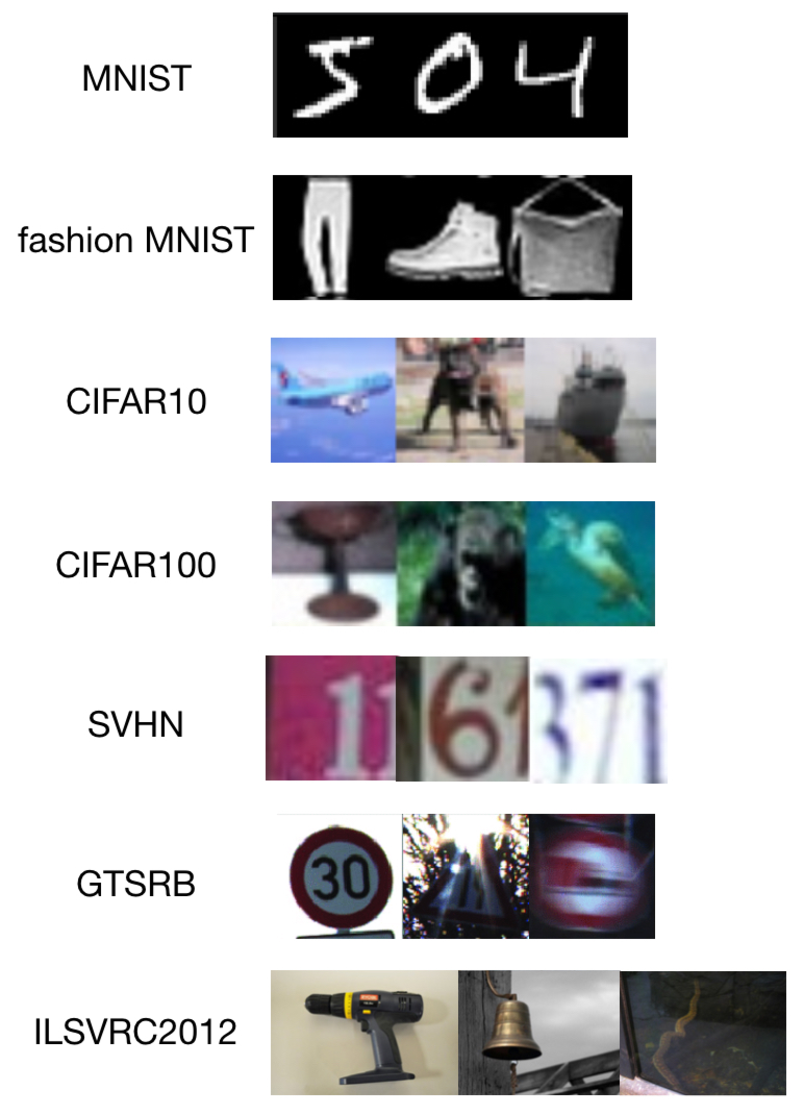
\includegraphics[width=8.0cm]{figures/typical-dataset-samples.pdf}
\end{center}
\caption{
典型的なデータセットのサンプル例.
画像はそれぞれのデータセットから引用.
}
\label{fig:typical-dataset-samples}
\end{figure}
%

\clearpage
\section{攻撃手法の各論}
\label{sec:attacks}
各攻撃手法について解説する.
よく知られているものやアイデアが特徴的な論文を独断と偏見で選んだ一覧が図 \ref{fig:attack-summary-table} である.
個人的に興味がある観点として攻撃対象が classifier なのか detector なのかを重視していたのでこれを基に上下に分けられているが, それ以外は出版年月順に並べている.
この章では基本的な手法となる FGSM 系手法とこの表の各手法について詳しく解説していく.
%
\begin{figure}[htbp]
\begin{center}
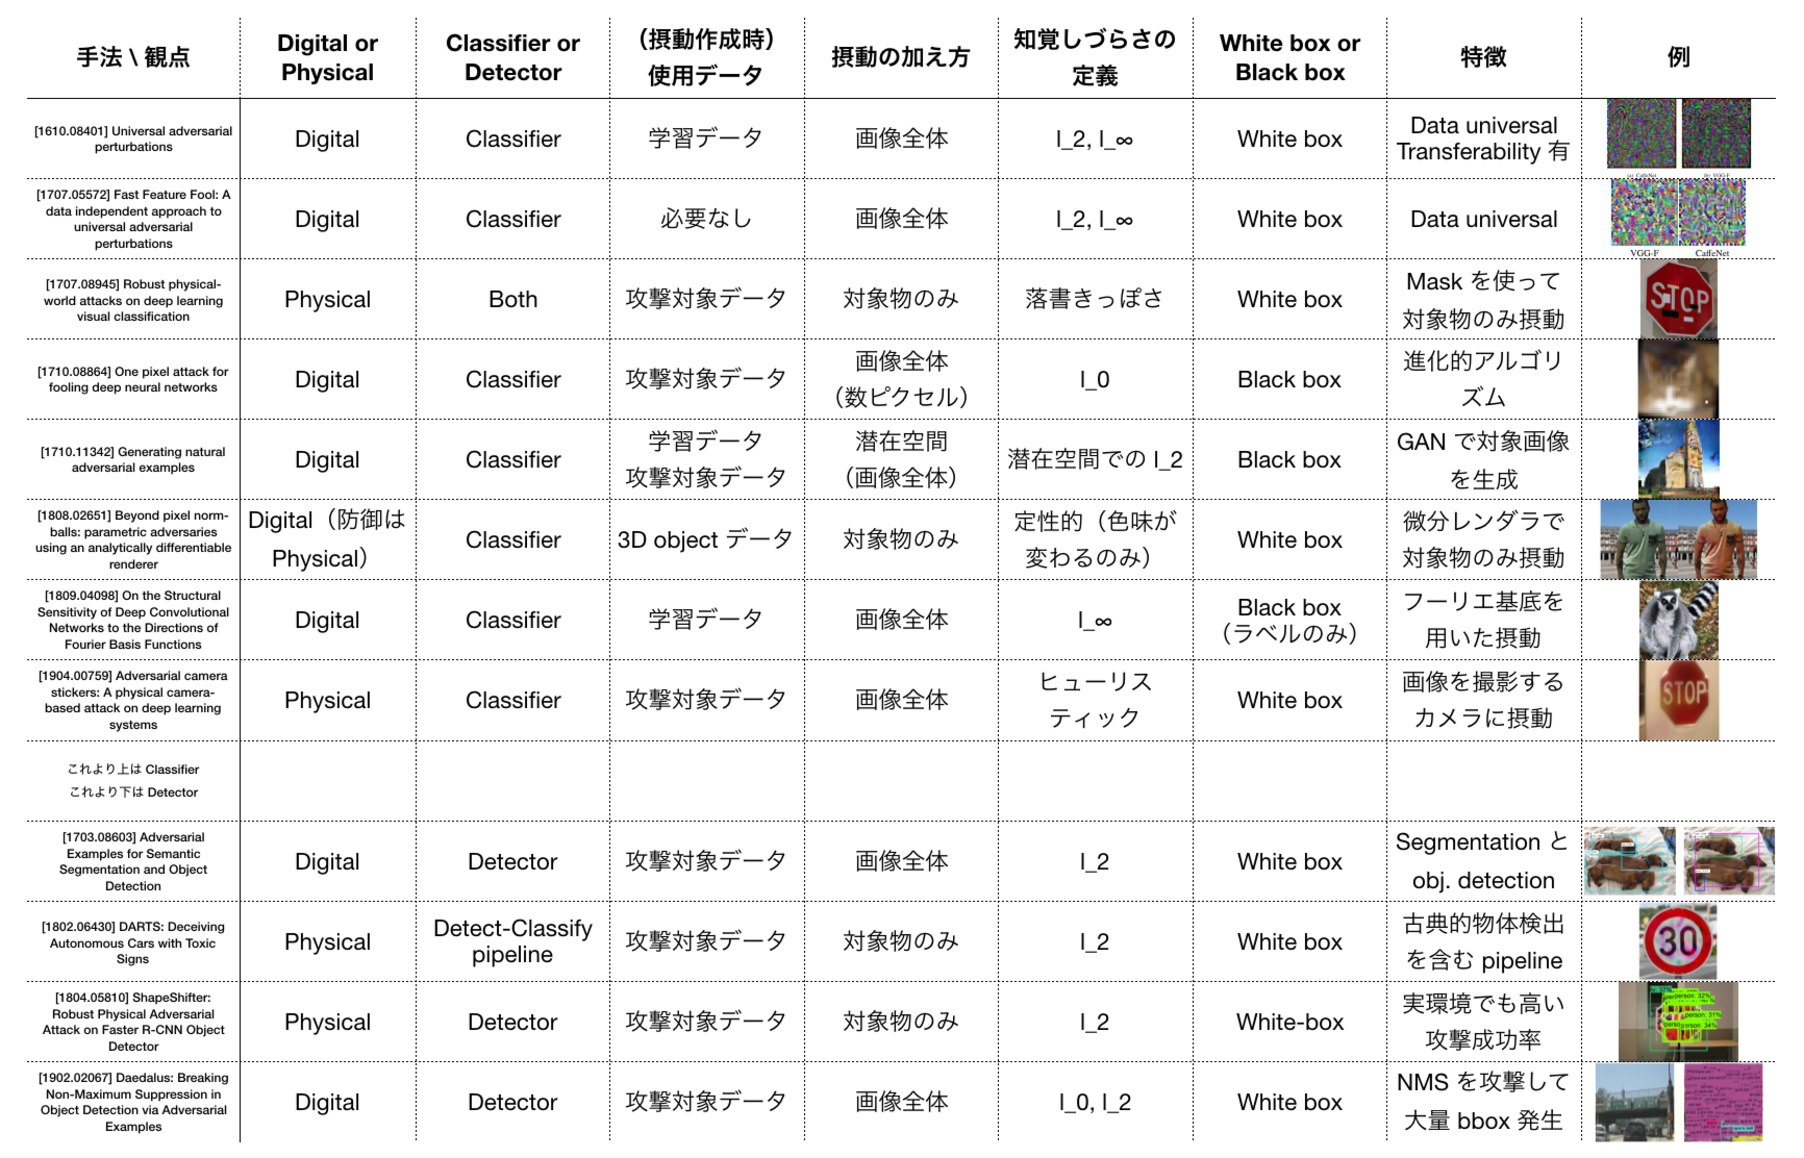
\includegraphics[width=16.0cm]{figures/attack-summary-table.pdf}
\end{center}
\caption{
本書で解説する攻撃手法の一覧とその特徴をまとめた表.
digital $\lor$ physical, classifier $\lor$ detector, 摂動作成時に使用するデータ, black box $\lor$ white box, 知覚しづらさの定義, 摂動の加え方, という観点で分類している.
個人的に重視している観点のため class ifier に対する手法と detector に対する手法を上下に分けて記載している.
文字が小さいため拡大して見ることを推奨.
}
\label{fig:attack-summary-table}
\end{figure}
%



\subsection{FGSM を基にした手法}
\label{subsec:fgsm-based}

\begin{table}[htbp]
\begin{center}
\begin{tabular}{|c|c|}
\hline
分類の観点 & この手法が該当するもの \\
\hline
Digital $\lor$ Physical & Digital \\
Classifier $\lor$ Detector & Classifier \\
摂動作成時に使用するデータ & 攻撃対象データ \\
摂動の加え方 & 画像全体 \\
知覚しづらさの定義 & $l_2$ もしくは $l_\infty$ \\
White box $\lor$ Black box & White box \\
\hline
\multicolumn{2}{|c|}{非公式実装: 検証実験のコードに含まれている} \\
\hline
\end{tabular}
\label{tb:fgsm-summary}
\end{center}
\end{table}

\ref{subsec:def-adv-examples} 節で既出であるが, adversarial examples を作成するための最も基本的な手法が FGSM である.
これは \cite{goodfellow2014explaining} によって提案された手法で, 一階微分に基づく手法であり広く使われている.

この手法は adversarial examples の初期に出たシンプルなものであり, この手法は多くの手法の基礎となったものである.
画像のピクセル値を任意に操作する Digital な攻撃で, 画像全体の情報を使ってラベルを予測する Classifier に対する攻撃である.
摂動は一枚の画像に対して対応する摂動を構築するようになっており, 画像と作成される adversarial example は一対一の関係にある.
摂動は画像全体に適用するので背景部分なども気にせず摂動を加えるようになっており, White box attack なのでモデルと loss function の情報を用いてモデルが誤認識しやすいように摂動を作成する.
人間にとっての知覚しづらさは摂動の $l_2$ や $l_{\infty}$ ノルムで測り, これらのノルムが小さければ摂動を加えた画像がその意味で元の画像から乖離が少なくなるため見分けがつきにくい, という方針である.
$l_{\infty}$ の方が定式化としてはすっきりとするため, $l_{\infty}$ の方を使うことが多い.

具体的な表式は式 \ref{eq:adv-fgsm} の繰り返しとなるが, adversarial examples の作り方は以下のようになっている.
%
\begin{eqnarray}
x_{\text{adv}} = x + \omega = x + \epsilon \cdot \text{sign} ( \nabla_x J (f, x, y_{\text{true}}) ).
\label{eq:adv-fgsm-again}
\end{eqnarray}
%
この手法が考案された背景は単純なものである.
重みベクトルを $w$ として $x_{\text{adv}}$ を以下のように分解することを考える.
%
\begin{eqnarray}
w^T x_{\text{adv}} = w^T x + w^T \omega.
\label{eq:adv_decompose}
\end{eqnarray}
%
一項目が摂動なしのもので二項目が摂動の効果であり, 摂動を小さく保ちつつ元の特徴からは大きく異なるものにしたいということを考えれば, $\epsilon$ の各要素の大きさは小さくしつつも $w^T$ との積は大きくするということになる.
各要素の大きさは $l_\infty$ で制限することにすると, この $\epsilon$ は $\epsilon = \epsilon \cdot \text{sign} (w)$ とするのがよいことが分かる.
このシンプルな考えをモデルに適用するには, 式 \ref{eq:adv-fgsm-again} のように loss function を $x$ で微分\footnote{
adversarial examples 作成時には重みベクトルは固定して, 変更するのは入力データである.
}して loss が大きくなるように正符号で元の $x$ に加えればよい (ただし $\epsilon > 0$ とする).
モデルの重みの更新の場合とは異なり, このデータの更新は一度だけ実施する.
この手法で構成された画像の例が図 \ref{fig:goodfellow-adv-example} である.
%
\begin{figure}[htbp]
\begin{center}
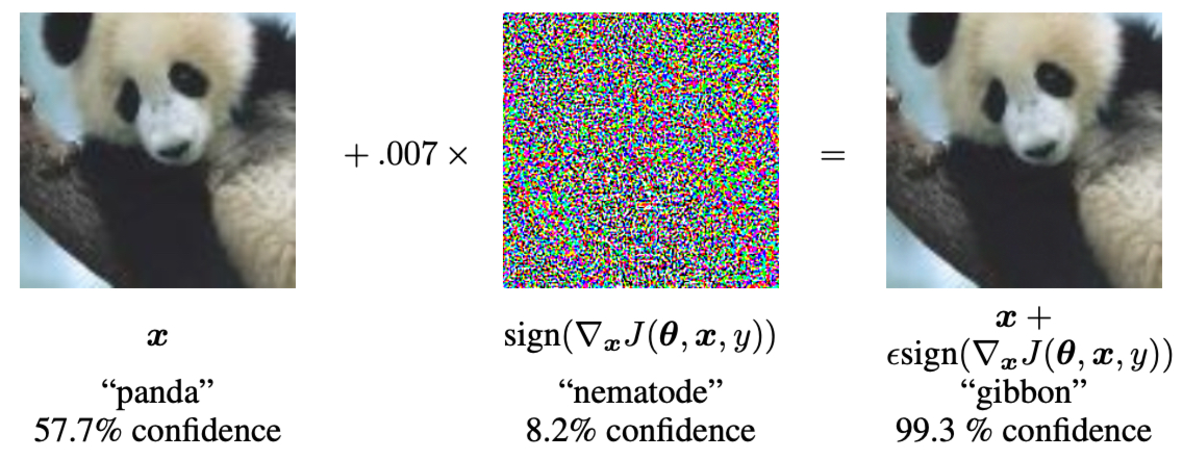
\includegraphics[width=12.0cm]{figures/goodfellow-adv-examples.pdf}
\end{center}
\caption{
FGSM で作成した adversarial examples の例.
攻撃対象としているモデルは GoogLeNet \cite{szegedy2015going} である.
左列が元画像, 中央列が作成した摂動, 右列が元画像に摂動を加えた画像である.
\textit{panda} と認識されていた画像が \textit{gibbon} (テナガザル) と誤認識されてしまっている.
図は \cite{goodfellow2014explaining} より引用.
}
\label{fig:goodfellow-adv-example}
\end{figure}
%

この構成法から明らかなように, この手法は white box attack であり, モデルの loss function とその微分情報がなければ使えないものである.
構成法がシンプルでありながら結果が興味深いものであり, 既存の DNN フレームワークで実装も容易であるため, その後の発展の礎になった手法であると共に現在もベースライン手法としてたびたび用いられる.

R+FGSM は FGSM にランダムなノイズの効果を入れることで後述する防御方法である adversarial training に有効な adversarial examples を作成しようとする手法である.
FGSM で作成した adversarial examples による loss function の形状は元データ近辺に局在していて大域的な最適化が困難になるため, ノイズを注入してそれを緩和するという目的で導入された.
まだ防御方法の紹介をしていないためここでは詳細は割愛するが, 手法としては以下のようにシンプルである.
%
\begin{eqnarray}
x_{\text{adv}} = x + \omega  = x + \alpha \cdot \text{sign} (\mathcal{N} (0^{m}, I^{m})) + (\epsilon - \alpha) \cdot \text{sign} (\nabla_x J (f_{\text{logit}}(x), y_{\text{true}})).
\label{eq:rfgsm}
\end{eqnarray}
%
ここで, $\mathcal{N} (0^{m}, I^{m})$ は $m$ 次元正規分布であり, $0 < \alpha < \epsilon$ である.
元論文では正規分布を用いているが, 符号のみが重要なので正負が等しい確率で得られればよいのでベルヌーイ分布や一様分布などでも同じ結果となる。

I+FGSM は元論文では PGD と呼称されている (本書では FGSM との関連性を明示するために I+FGSM と書く).
Iterative という名前から想像されるように, FGSM を繰り返し適用する手法となっている.
ただし, 繰り返し適用することで摂動が大きくなってしまう可能性があるため, 摂動が大きくなりすぎないように一定範囲に収まるように射影するというものになっている.
合計 $K$ 回の繰り返しをしてその途中の $t$ 回目の adversarial examples を $x_{\text{adv}}^t$ と書くとき, I+FGSM は以下のように書ける.
%
\begin{eqnarray}
\begin{aligned}
x_{\text{adv}}^{(0)} &= x \\
x_{\text{adv}}^{(t + 1)} &= x_{\text{adv}}^{(t)} + \alpha \cdot \text{sign} (\nabla_x J (f, x_{\text{adv}}^{(t)}, y_{\text{true}})) \\
x_{\text{adv}}^{(t + 1)} &= \text{clip} (x_{\text{adv}}^{(t + 1)}, x - \omega, x + \omega) \\
x_{\text{adv}} &= x_{\text{adv}}^{(K)}
\end{aligned}
\label{eq:ifgsm}
\end{eqnarray}
%
ここで, $\text{clip} (x, x_{\text{min}}, x_{\text{max}})$ は入力 $x$ を $[x_{\text{min}}, x_{\text{max}}]$ に射影する elementwise に適用される関数である.

MI+FGSM は I+FGSM の改良版であり, 前のステップでの微分情報に decay factor $\mu$ を掛けて momentum として使用して更新する手法である.
%
\begin{eqnarray}
\begin{aligned}
x_{\text{adv}}^{(0)} &= x \\
g^{(0)} &= 0 \\
g^{(t + 1)} &= \mu g^{(t)} + \frac{\nabla_x J (f, x_{\text{adv}}^{(t)}, y_{\text{true}})}{\|\nabla_x J (f, x_{\text{adv}}^{(t)}, y_{\text{true}})\|_1} \\
x_{\text{adv}}^{(t + 1)} &= x_{\text{adv}}^{(t)} + \alpha \cdot \text{sign} (g^{(t + 1)}) \\
x_{\text{adv}}^{(t + 1)} &= \text{clip} (x_{\text{adv}}^{(t + 1)}, x - \omega, x + \omega) \\
x_{\text{adv}} &= x_{\text{adv}}^{(K)}
\end{aligned}
\label{eq:mifgsm}
\end{eqnarray}
%
この手法は 2017 NIPS Adversarial Attacks Competition で一位を獲得した手法である.



\subsection{Universal adversarial perturbations}
\label{subsec:universal-adversarial}
%
\begin{table}[htbp]
\begin{center}
\begin{tabular}{|c|c|}
\hline
分類の観点 & この手法が該当するもの \\
\hline
Digital $\lor$ Physical & Digital \\
Classifier $\lor$ Detector & Classifier \\
摂動作成時に使用するデータ & 学習データ全体 \\
摂動の加え方 & 画像全体 \\
知覚しづらさの定義 & $l_2, l_{\infty}$ \\
White box $\lor$ Black box & White box \\
\hline
\multicolumn{2}{|c|}{公式実装: \href{https://github.com/LTS4/universal}{https://github.com/LTS4/universal}} \\
\hline
\end{tabular}
\label{tb:universal-adversarial-summary}
\end{center}
\end{table}
%

これは \cite{moosavi2017universal} によって提案された手法であり, 概要は図 \ref{fig:universal-adversarial-summary} のようになっており, 様々なクラスの画像に対して単一の摂動を加えることで異なるクラスに誤認識させることに成功している.
%
\begin{figure}[htbp]
\begin{center}
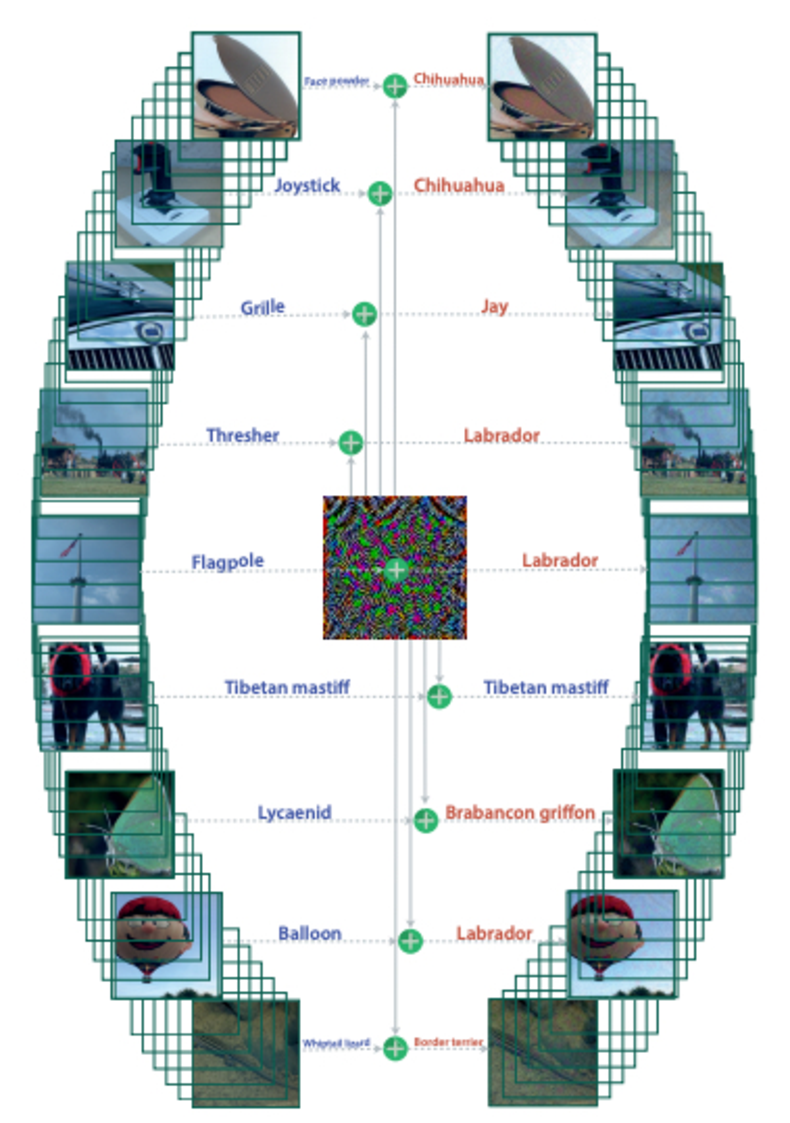
\includegraphics[width=10.0cm]{figures/universal-adversarial-summary.pdf}
\end{center}
\caption{
手法の概要.
左側の画像とラベルが元画像とモデルによって予測される正しいラベルで, 中央にある単一の摂動をそれぞれの画像に加えることで, 右側の画像になり予測ラベルも変わる (赤字は正しくないラベルで誤認識されたことを示す).
図は \cite{moosavi2017universal} より引用.
}
\label{fig:universal-adversarial-summary}
\end{figure}
%

この手法はの特徴は摂動を作成する際に学習データ全体を使用することにあり, 多様なデータを用いることで, 攻撃時にも多様なデータに対して有効な普遍的な一つの摂動を作成することに成功している.
基本的なアイデアは, あるデータに対して誤認識させるために識別領域を超えるような摂動を作成し, それを一定の大きさに保ちながら各データに対して繰り返し適用するというものである.
それ以外の観点は FGSM と同様である.

この手法が登場するまでは, 一枚の攻撃対象となる画像データに対して摂動を作成するというものが殆どだったが, この手法が目指すところは摂動として普遍的 (ここでは攻撃対象となる画像に依らないという意味) なものの作成である.
実現したい状況を定式化すると以下のようになる.
$x$ は集合 $\mathcal{X}$ に属する様々なデータとなるが, 摂動である $\omega$ は $x$ に依らない単一の量であることに注意されたい.
%
\begin{eqnarray}
f_{\text{label}} (x + \omega) \neq f_{\text{label}} (x) \ \ \text{for "most" } x \in \mathcal{X}.
\label{eq:universal-adversarial-formulation}
\end{eqnarray}
%
論文では $x \sim  \mu$ としてデータ $x$ を生成する確率分布 $\mu$ を用いているが, 当然これは直接は扱えないものであるため, ここでは入力データ集合に置き換えている.
この段階では摂動の大きさに制限がないのと, 「most」 の意味するところが抽象的であるので, それを明示的に取り入れるため以下の条件を課す.
%
\begin{enumerate}
  \item $\|\omega\|_{p} \leq \epsilon.$
  \item $\text{Err}_{x \in \mathcal{X}} \left( f_{\text{label}} (x + \omega) \neq f_{\text{label}} (x)  \right) \geq 1 - \delta.$
\end{enumerate}
%
2 つ目の条件は誤認識させる割合が $1 - \delta$ であることを意味している.
目的はこの $(\epsilon, \delta)$ として共に小さい値を実現するようなアルゴリズムを構築すること, と言い換えることができる.

そうは言っても使用する技術的な道具は FGSM の場合とそう大きくは変わらない.
アルゴリズム \ref{alg:universal-adversarial-alg} に全体像を示す.
摂動を更新する際のコアとなる手法は FGSM などの先行研究の手法を用いるものになっており, 論文では DeepFool \cite{moosavi2016deepfool} を用いている\footnote{
これは FGSM を iterative に改良した手法で, 各ステップで勾配情報から摂動 $\omega_i$ を作成し, 次のステップで $x + \omega_i$ で同様の操作を実施して最終的に $\omega = \sum \omega_i$ とする.
I+FGSM との違いは I+FGSM は毎回 $\omega$ 全体を更新しているが, DeepFool では各ステップの変位を残しておいて最後にそれを足すという点にある.
攻撃性能は I+FGSM の方が高いが, ベースライン手法として DeepFool もたびたび用いられる.
}.
各データ毎に摂動を作成してそれを加えていくことで摂動の大きさが増大していく可能性があるため, $l_p$ ノルム の値が $\epsilon$ 以下という条件の下で $l_2$ ノルムの意味で最適な摂動に近づくように制限を加えている.
あとはこの手続きを所望の誤認識率を達成するまで繰り返せばよい.
注意すべき点として, このアルゴリズムはモデルに依存するのはもちろんのこと, データ集合 $\mathcal{X}$ を固定してもループの順番によって最終的に得られる摂動が変わるということが挙げられる.
%
\begin{algorithm}
\caption{Universal Adversarial Perturbations のアルゴリズム}
\label{alg:universal-adversarial-alg}
\begin{algorithmic}[1]
    \State Input: データ集合 $\mathcal{X}$, モデル $f_{\text{label}}$, $l_p$ノルムとその大きさの制限 $\epsilon$, 誤認識率を測る
    $\delta$
    \State Output: 摂動 $\omega$
	\State 摂動を初期化: $\omega \leftarrow 0$
	\While {$\text{Err}_{x \in \mathcal{X}} \left( f_{\text{label}} (x + \omega) \neq f_{\text{label}} (x)  \right) \leq 1 - \delta.$}
	\For {各データ $x_i \in \mathcal{X}$}
	\If {$f_{\text{label}} (x_i + \omega) = f_{\text{label}} (x_i)$}
	\State 誤認識をさせるために必要な最小限の摂動を計算 (FGSM などの先行研究の手法を用いる): $\Delta \omega_i \leftarrow \argmin_{r} \left[\|r\|_2\right] \ \text{s.t.} \  f_{\text{label}} (x_i + \omega + r) \neq f_{\text{label}} (x_i).$ 
	\State 摂動を更新: $\omega \leftarrow \argmin_{\omega'} \left[ \|(\omega + \Delta \omega_i) - \omega'\|_2 \right] \ \text{subjet to} \ \|\omega'\|_p \leq \epsilon.$
	\EndIf
	\EndFor
	\EndWhile
\end{algorithmic} 
\end{algorithm}
%

ILSVRC2012 \cite{russakovsky2015imagenet} データを用いた実験結果を見ていこう.
実験に使用しているモデルは以下の通りで, 論文出版時の主要なモデルが取り上げられている.
%
\begin{itemize}
  \item CaffeNet \cite{jia2014caffe}
  \item VGG-F \cite{chatfield2014return}
  \item VGG \cite{simonyan2014very}
  \item GoogLeNet \cite{szegedy2015going}
  \item ResNet \cite{he2016deep}
\end{itemize}
%

まずは摂動を作成するために 10,000 件のデータを用いて, 検証用に 50,000 件使用した結果が図 \ref{fig:universal-adversarial-result-table} である.
どのモデルにおいても $\mathcal{X}$ でも検証用データでも同程度の誤認識率となっており, 作成した摂動は $\mathcal{X}$ のみに過学習しているわけではないことが分かる (元が同じデータセットなのでそこまで強い主張にはなり得ないが).
また, $l_2, l_\infty$ ノルムのどちらが適しているかはモデルによって異なる.
大きな傾向として, モデルの層の数などが少ない簡単なモデルの方が誤認識率が高いことが伺える.
%
\begin{figure}[htbp]
\begin{center}
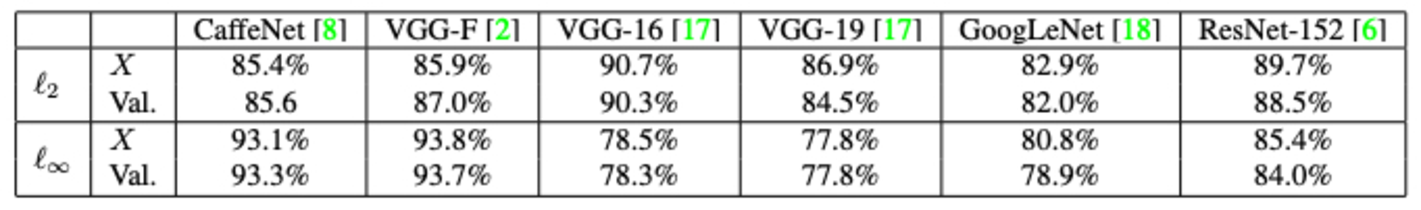
\includegraphics[width=14.0cm]{figures/universal-adversarial-result-table.pdf}
\end{center}
\caption{
摂動を作成したデータと検証用のデータそれぞれでの誤認識率を比べたもの.
$l_2$, $l_{\infty}$ の制限としてそれぞれ $\epsilon = 2000, \epsilon = 10$ を用いている.
図は \cite{moosavi2017universal} より引用.
}
\label{fig:universal-adversarial-result-table}
\end{figure}
%

次にモデル毎に得られた普遍的な摂動を示したものが図 \ref{fig:universal-adversarial-perturbations-models} である.
モデル毎に人間にとっても大きく見た目が異なる摂動が得られている.
%
\begin{figure}[htbp]
\begin{center}
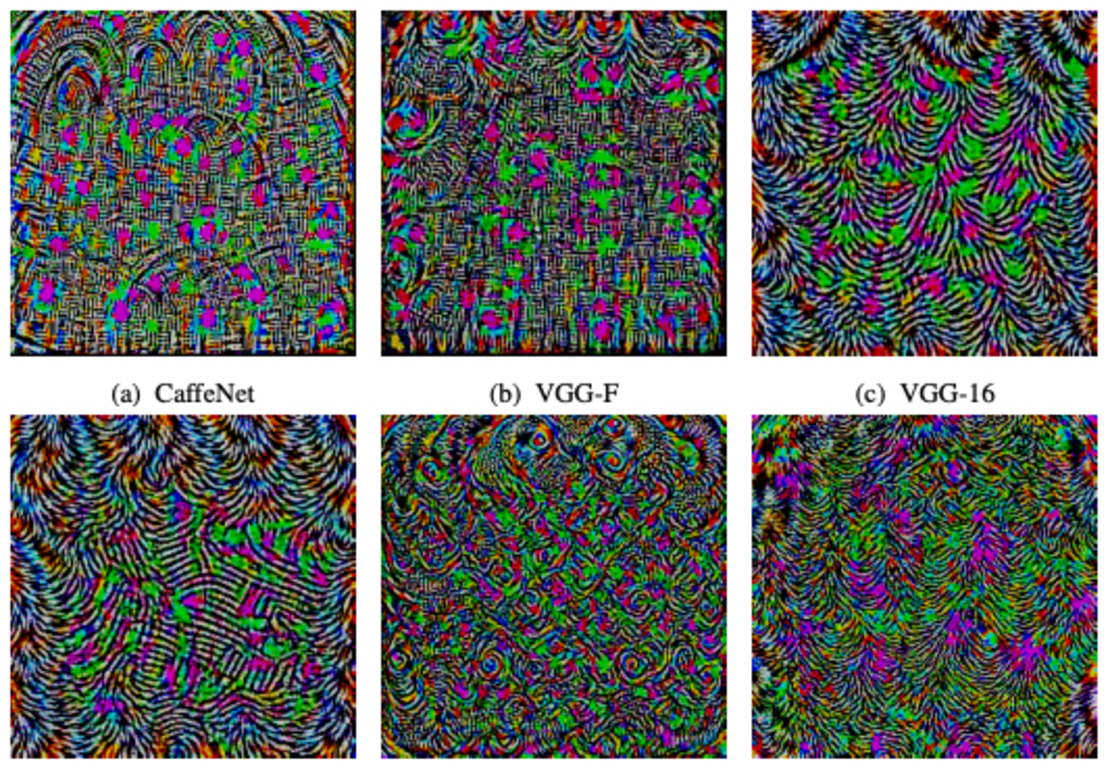
\includegraphics[width=10.0cm]{figures/universal-adversarial-perturbations-models.pdf}
\end{center}
\caption{
モデル毎に得られた普遍的な摂動.
図は \cite{moosavi2017universal} より引用.
}
\label{fig:universal-adversarial-perturbations-models}
\end{figure}
%

この手法はデータの順番に依存するものであることを言及していたが, データ順を変えた場合に結果がどう変わるかを示したものが図 \ref{fig:universal-adversarial-perturbations-shuffle} である。
モデルは GoogLeNet を使用していて, 人間の目には似通った模様に見えるが, 正規化した内積の値は 0.1 以下であり, 普遍的な摂動はデータ順に依存して unique なものではないことが示されている.
%
\begin{figure}[htbp]
\begin{center}
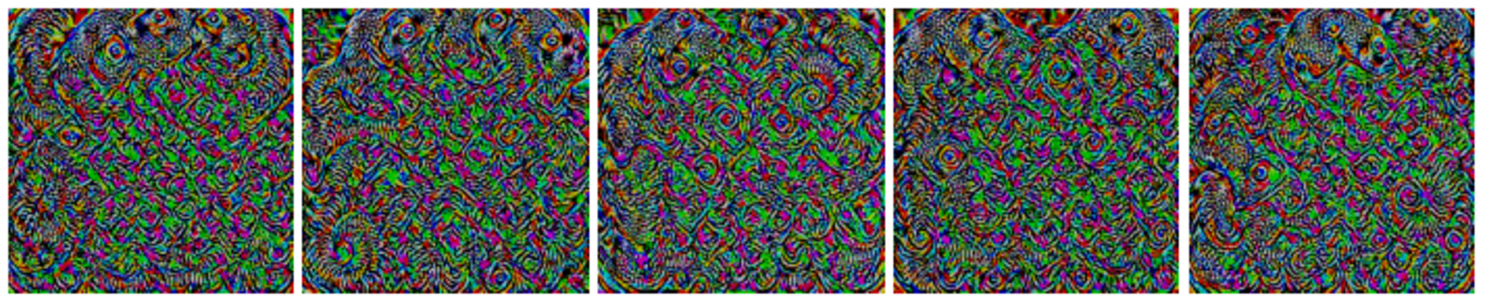
\includegraphics[width=14.0cm]{figures/universal-adversarial-perturbations-shuffle.pdf}
\end{center}
\caption{
データ順をシャッフルし GoogLeNet で異なる普遍的な摂動を求めた結果.
それぞれの正規化した内積を計算すると値は 0.1 以下となり, 人間の目では似通って見えるが異なる摂動になっている.
図は \cite{moosavi2017universal} より引用.
}
\label{fig:universal-adversarial-perturbations-shuffle}
\end{figure}
%

ここまでの結果で, 提案手法の目的であった個別のデータに依らない普遍的な摂動というのが確かに構築できる (しかし unique ではない) ということが示された.
それだけに留まらず, あるモデルで作成した摂動が他のモデルでも一定度の有効性があることも示されている.
その結果が図 \ref{fig:universal-adversarial-transferability} であり, このように別モデルに対しても有効であることを adversarial examples に transferability があると言う.
この論文が発表されて以降, adversarial examples の transferability に関して様々な進展が報告されるようになった.
モデルの構造が似通っていると高い transferability を達成していることが見て取れる.
%
\begin{figure}[htbp]
\begin{center}
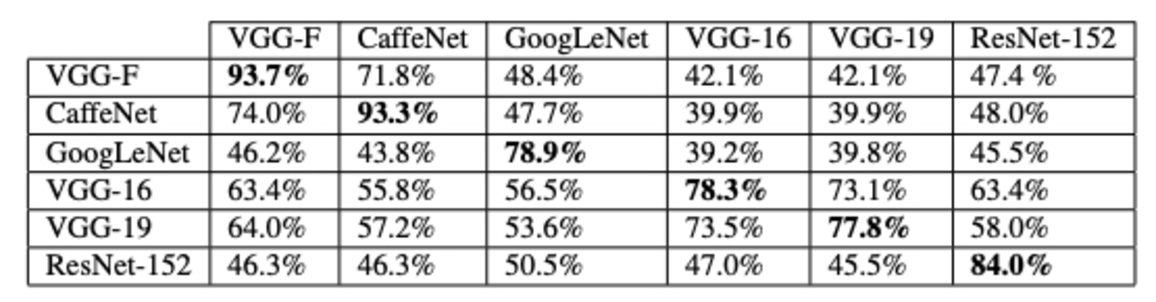
\includegraphics[width=14.0cm]{figures/universal-adversarial-transferability.pdf}
\end{center}
\caption{
adversarial examples の transferablity を調べた結果.
各行が普遍的な摂動を作成するのに使用したモデルで, 各列が誤認識率を計算したモデルになっている.
図は \cite{moosavi2017universal} より引用.
}
\label{fig:universal-adversarial-transferability}
\end{figure}
%

なぜ単一の普遍的な摂動が有効なのかというのが疑問として残るが, 論文では識別境界付近は比較的少数のベクトルで span される低次元空間で記述されているのではないかという仮説に基づいてデータ点での識別境界への法線ベクトルの解析を実施している.
CaffeNet において, 以下で定義される識別境界への法線ベクトルを集めた行列を求める.
%
\begin{eqnarray}
N = \left[ \frac{\omega(x_1)}{\|\omega(x_1)\|_2}, \dots, \frac{\omega(x_{|\mathcal{X}|})}{\|\omega(x_{|\mathcal{X}|})\|_2} \right] \ \text{where} \ \argmin_{\omega} \left[ \|\omega\|_2 \right] \ \text{s.t.} \ f_{\text{label}} (x + \omega) \neq f_{\text{label}} (x).
\label{eq:universal-adversarial-normalvect}
\end{eqnarray}
%
この行列の特異ベクトルと単位球からランダムサンプルした特異ベクトルを比較する.
その結果が図 \ref{fig:universal-adversarial-singular-values} で, 確かに識別境界への法線ベクトルは少数のベクトルの寄与が大きく有効次元が低いことが示されている.
この論文ではこのようなある種の状況証拠のような解析までしか実施されていないが, 後の論文で識別境界付近の曲率に注目し, 線形もしくは条件付きの非線形の識別境界の場合に普遍的な摂動に弱いことが報告されている\cite{moosavi2017analysis}.
%
\begin{figure}[htbp]
\begin{center}
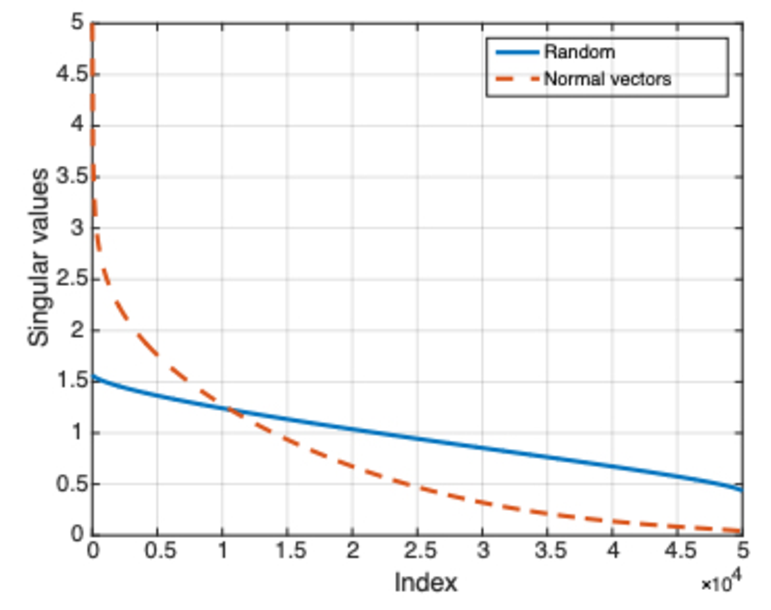
\includegraphics[width=8.0cm]{figures/universal-adversarial-singular-values.pdf}
\end{center}
\caption{
識別境界への法線ベクトルをまとめた行列の特異値分布と単位球からランダムサンプルした場合の特異値分布を比較した結果.
縦軸は特異値の大きさで横軸は特異値を大きい順に並べたときの index である.
識別境界付近の空間が少数の特異ベクトルで記述されていることを示している.
図は \cite{moosavi2017universal} より引用.
}
\label{fig:universal-adversarial-singular-values}
\end{figure}
%

その他にも, 誤認識されるクラスは等しく分布するのではなく特定のクラスに偏る傾向にあるという性質とそのグラフ理論的な解析の方向性も言及されているが, この点に関してその後詳しく調べられているかは著者は知らない.

この手法は示唆に富むものであったので, その後の様々な発展につながっている.
特に, adversarial examples の transferability に関して, 現実的に攻撃する際には (攻撃対象のモデルの情報は取得できないことが殆どなので)  black box attack を用いる必要があるが, 手元で white box の手法で作成した adversarial examples を攻撃に転用するのが主流となった.



\subsection{Fast Feature Fool: A data independent approach to universal adversarial perturbations}
\label{subsec:fast-feature}
%
\begin{table}[htbp]
\begin{center}
\begin{tabular}{|c|c|}
\hline
分類の観点 & この手法が該当するもの \\
\hline
Digital $\lor$ Physical & Digital \\
Classifier $\lor$ Detector & Classifier \\
摂動作成時に使用するデータ & モデル情報のみでデータは必要なし \\
摂動の加え方 & 画像全体 \\
知覚しづらさの定義 & $l_{\infty}$ \\
White box $\lor$ Black box & White box \\
\hline
\multicolumn{2}{|c|}{公式実装: \href{https://github.com/val-iisc/fast-feature-fool}{https://github.com/val-iisc/fast-feature-fool}} \\
\hline
\end{tabular}
\label{tb:fast-feature-summary}
\end{center}
\end{table}
%

これは \cite{mopuri2017fast} によって提案された手法であり, データに依らずにモデルの各層の出力の平均値が大きくなるような摂動を作成することで誤認識を引き起こす手法である.

摂動作成時に使用するデータ以外は FGSM や Universal Adversarial Perturbation と変わらないが, 摂動を作成する際にモデルの情報のみを使いデータを全く使わないのが特徴である.
モデルによる予測はある層の出力に変換を施してそれを次の層に渡してということを繰り返していくが, 各層の出力が入力データに関わらずに大きくなるような摂動が作成できれば, 入力データの特徴が無視されるほど摂動の影響が大きくなり, 誤認識を引き起こすことが可能になると考えられる.
そのような摂動は学習済みモデルがあれば作成することができるので, それを実際にやってみたのがこの手法となる.

摂動を適当に初期化して, 層 $i$ の出力の平均を $\bar{l}_i$ として以下のように loss function を設定する.
%
\begin{eqnarray}
J(f, \omega) = - \log \left(\prod_{i = 1}^{\text{\# of layers}} \bar{l}_i (\omega) \right) \ \text{s.t.} \ \|\omega\|_p < \epsilon.
\label{eq:fast-feature-loss}
\end{eqnarray}
%
出力は基本的には ReLU の出力を使用することを想定しているので非負であり, fully connected layer より手前の convolutional layer を $i$ として採用している\footnote{
実装を見ると途中の pooling layer も含めているように読み取れるのでその限りではない.
詳しくは実装を参照のこと.
}.

提案手法としては以上で, あとは Universal Adversarial Perturbations と同様に ILSVRC2012 と各種モデルを使った実験に入る.
摂動の大きさとして $\epsilon = 10$ を用いており, これは Universal Adversarial Perturbations と同じ値である.
まず, ILSVRC2012 で学習した各モデルから得られた摂動は図 \ref{fig:fast-feature-perturbations} である.
Universal Adversarial Perturbations の結果と比べるとより特定の模様が強調されているようにも見えるが, そこに何かしらの意味があるのかは論文では言及されておらず, 著者にも分からない.
%
\begin{figure}[htbp]
\begin{center}
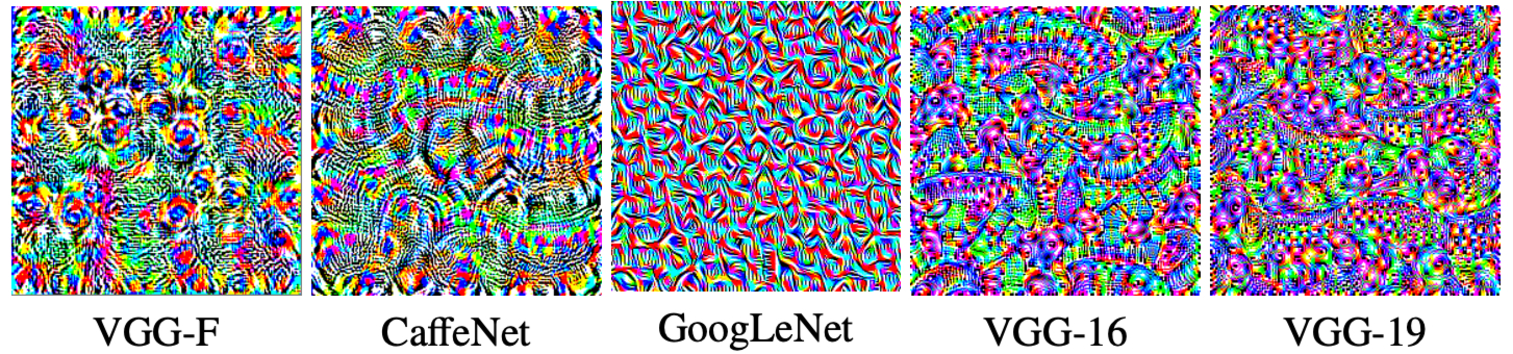
\includegraphics[width=14.0cm]{figures/fast-feature-perturbations.pdf}
\end{center}
\caption{
モデル毎に得られた摂動.
図は \cite{mopuri2017fast} より引用.
}
\label{fig:fast-feature-perturbations}
\end{figure}
%

得られた摂動を用いて誤認識率を調べたものが図 \ref{fig:fast-feature-transferability} である.
具体的なデータを使っていないため Universal Adversarial Perturbations よりは誤認識率 (図 \ref{fig:universal-adversarial-transferability} を参照) が低くなっているが, それでも高い誤認識率を達成していることが示されている.
%
\begin{figure}[htbp]
\begin{center}
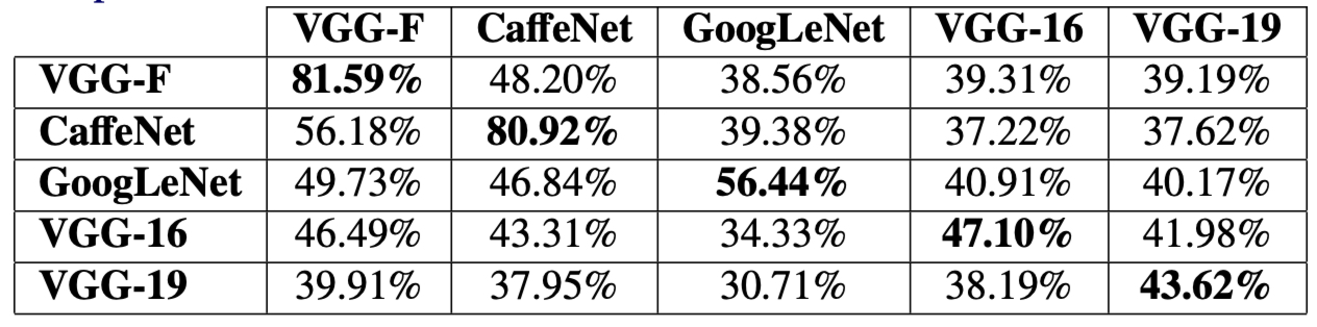
\includegraphics[width=14.0cm]{figures/fast-feature-transferability.pdf}
\end{center}
\caption{
ILSVRC2012 で学習したモデルから作成した摂動を用いて, 検証用のデータで誤認識率を調べた結果.
各行が摂動を作成したモデルで, 各列が誤認識率を評価したモデルになっている.
図は \cite{mopuri2017fast} より引用.
}
\label{fig:fast-feature-transferability}
\end{figure}
%

GoogLeNet で得られた摂動を用いて予測結果がどのように変化するかをサンプリングしたものが図 \ref{fig:fast-feature-examples} である.
拡大して見ることで確かに摂動が載っていることが分かる.
%
\begin{figure}[htbp]
\begin{center}
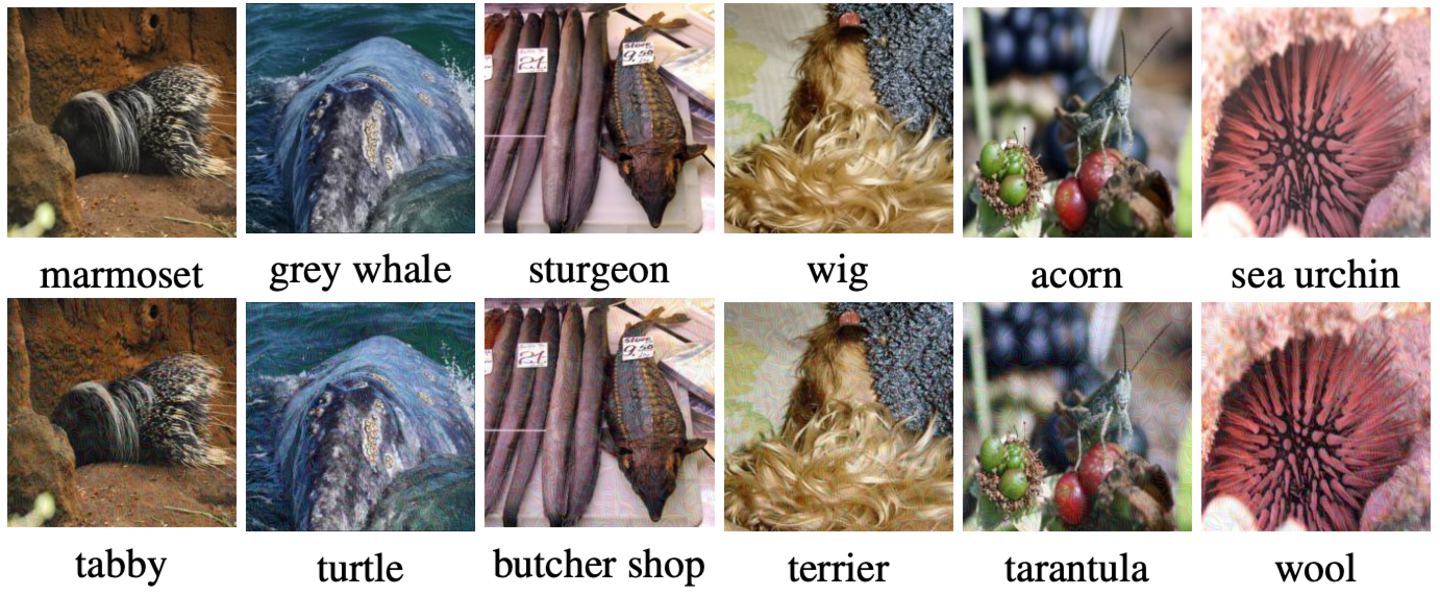
\includegraphics[width=14.0cm]{figures/fast-feature-examples.pdf}
\end{center}
\caption{
GoogLeNet における具体例.
上の行が元データと (正しく予測されている) ラベルで, 下の行が adversarial examples と誤認識されたラベルである.
図は \cite{mopuri2017fast} より引用.
}
\label{fig:fast-feature-examples}
\end{figure}
%

この論文では新たに adversarial examples のデータ間の transferability についても検証している.
具体的には ILSVRC2012 で学習したモデルで作成した摂動を Places-205 \cite{zhou2016places} の検証用データに加えて, Places-2015 で学習したモデルがどれくらい誤認識するかを調べている.
結果が図 \ref{fig:fast-feature-data-transferability} であり, ある程度はデータ間の transferability が存在することが示されている.
提案手法はかなり誤認識率が低いが Universal Adversarial Perturbations では高いことから, 提案手法はかなりデータに特化した摂動で Universal Adversarial Perturbations に関してはある程度物体の普遍的な特徴に対する摂動となっていると考えられる.
%
\begin{figure}[htbp]
\begin{center}
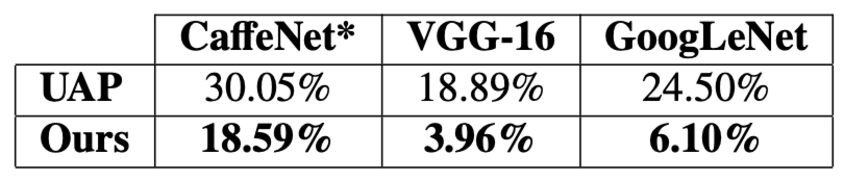
\includegraphics[width=10.0cm]{figures/fast-feature-data-transferability.pdf}
\end{center}
\caption{
adversarial examples に対してデータの transferability を調べた結果.
ILSVRC2012 で学習したモデルで作成した摂動を使って Places-205 のデータセットで検証をしている.
UAP は Universarial Adversarial Perturbations を意味しており, CaffeNet のスターは実際には誤認識率を計算する際に AlexNet を用いていることを意味している (2 つのアーキテクチャは似ているが少し異なっている).
図は \cite{mopuri2017fast} より引用.
}
\label{fig:fast-feature-data-transferability}
\end{figure}
%

この手法は摂動作成時はデータを用いないという点で興味深いものだが, 学習に用いたデータへの依存性が強い.
このような研究と Universal Adversarial Perturbations と合わせることで, 様々な transferability の可能性が認識されるようになった.



\subsection{Robust Physical-World Attacks on Deep Learning Models}
\label{subsec:robust-physical}
%
\begin{table}[htbp]
\begin{center}
\begin{tabular}{|c|c|}
\hline
分類の観点 & この手法が該当するもの \\
\hline
Digital $\lor$ Physical & Physical \\
Classifier $\lor$ Detector & Classifier (後に Detector にも有効であることを示した) \\
摂動作成時に使用するデータ & 攻撃対象クラスのデータ 1 枚 \\
摂動の加え方 & 対象物のみ \\
知覚しづらさの定義 & 落書きっぽさ \\
White box $\lor$ Black box & White box \\
\hline
\multicolumn{2}{|c|}{公式実装: \href{https://github.com/evtimovi/robust_physical_perturbations}{https://github.com/evtimovi/robust\_physical\_perturbations}} \\
\hline
\end{tabular}
\label{tb:robust-physical-summary}
\end{center}
\end{table}
%

これは \cite{eykholt2018robust} によって提案された手法であり, 概要は図 \ref{fig:robust-physical-summary} のようになっており, 止まれの標識を速度制限の標識に誤認識させるような摂動を作成している.
%
\begin{figure}[htbp]
\begin{center}
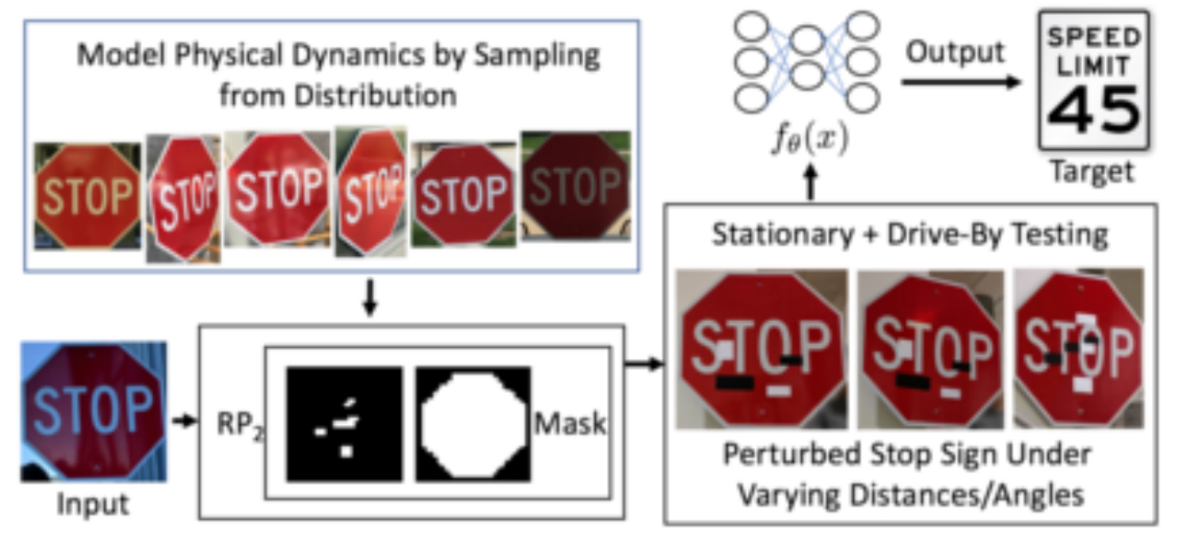
\includegraphics[width=12.0cm]{figures/robust-physical-summary.pdf}
\end{center}
\caption{
手法の概要.
標識のみに摂動を加えるような mask を作成し, 角度や明るさなどの条件を変更するような変換を適用したデータを用いて誤ったラベルに対する誤差が小さくなるような摂動を作成する.
図は \cite{eykholt2018robust} より引用.
}
\label{fig:robust-physical-summary}
\end{figure}
%

この手法は physical な攻撃であり, 標識に摂動を加えた画像をプリントしてそれを実際の標識に上から貼るというような手法になっている (本当に標識の上に印刷物を貼るのは違法なので, 実験では印刷物を室外環境で適当なところに貼って撮影して評価している).
摂動の作成はデジタル上で実施して, それをプリントして使用するため, 摂動作成時にはプリンターで実現可能な色味にできるだけ近づけるような拘束条件も導入している.

この攻撃の対象は classifier のみで画像中に単一の標識のみが映っているという状況を想定しており, そのため扱うデータも標識のみを切り出したものを使用する.
この論文の手法を detector にも適用できるように発展させた technical note を publish している \cite{eykholt2017note}.
この technical note では図 \ref{fig:robust-physical-detector} のようにある標識を別の標識に誤認識させるという手法ではなく標識を認識させず別の物体に誤認識させる手法だが, このような発展を通じて detector にも有効な adversarial examples が数多く報告されるようになってきている.
%
\begin{figure}[htbp]
\begin{center}
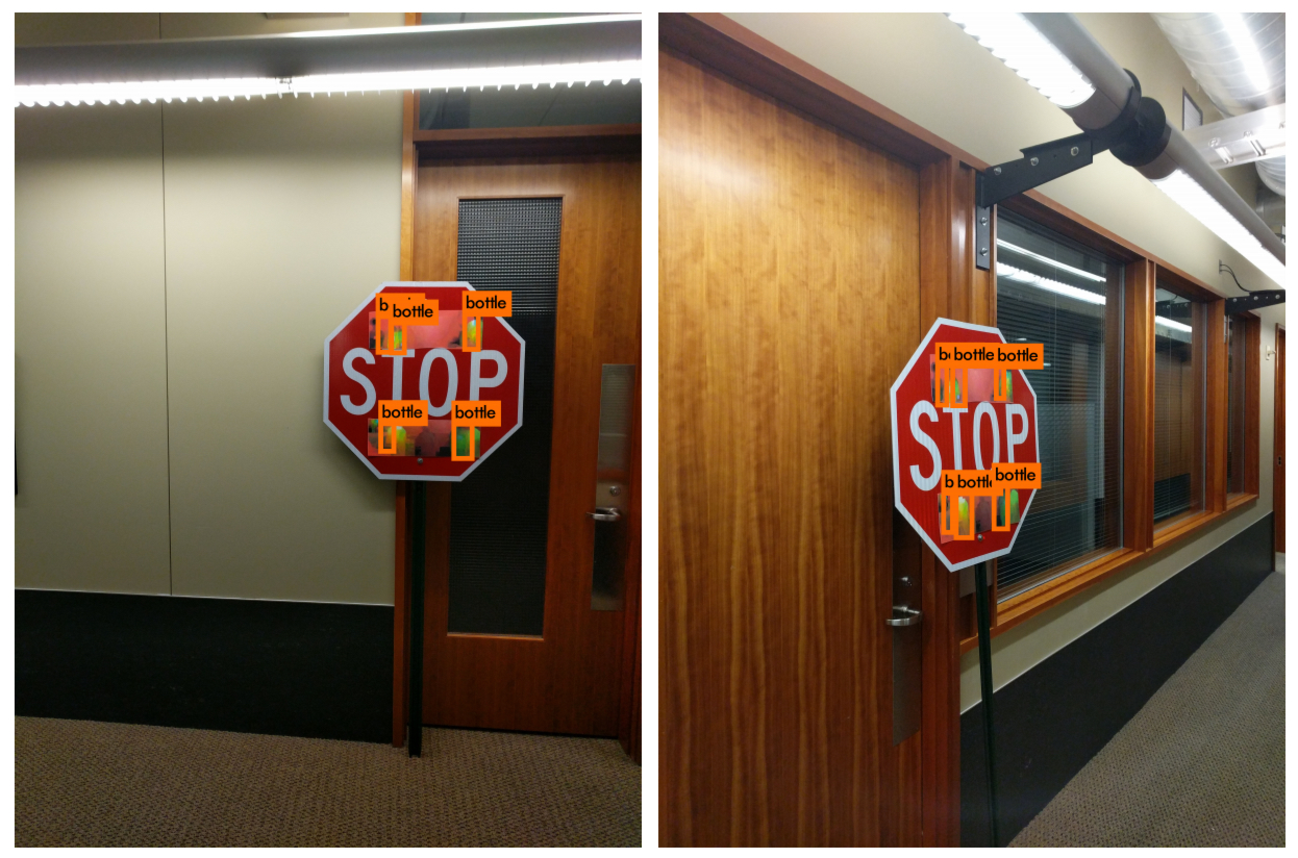
\includegraphics[width=12.0cm]{figures/robust-physical-detector.pdf}
\end{center}
\caption{
提案手法を detecotr に適用した結果.
図は \cite{eykholt2017note} より引用.
}
\label{fig:robust-physical-detector}
\end{figure}
%

摂動を作成する時は攻撃対象となるクラスの画像を一枚使用する.
道路標識は色々な距離や角度から撮影されるため, 摂動はそのような状況でも効果を発揮する必要がある.
そのため, その一枚に幾何学変換や輝度変換などを加えてデータセットを構築し, 対象となるクラスに有効な一つの摂動を作成する.
一クラスに対して一つの adversarial example を作るというものになっている.

この手法は white box に属するもので, モデルと loss function を与えて, loss function の値に基づいてモデルが誤認識をしやすいようにデータに摂動を加えていく.
標識外の部分に摂動を加えても撮影条件が変わればその効果は期待できないため, この手法では摂動を作成する際に標識以外の部分に mask  (この手法は攻撃対象のクラスの画像が一枚あれば作成できるため, それに合わせた mask を事前に準備している) を加えて標識部分だけで摂動を作成するようにしている.

知覚しづらさとして, 標識に落書きをしたような摂動になるために人間が adversarial examples と気付きにくいだろうというアイデアを採用している.
摂動自体は $l_1$ や $l_2$ ノルムを使って構築していくが, 様々な物理的環境で有効な摂動を作ろうとするとどうしても元画像からの差分は目につくようになる.
標識にスプレーなどで落書きをしたように見えるので知覚しづらい, というのはやや詭弁にも聞こえるが発想自体はなかなか面白いものであり, この考え方を推し進めて虫がついてるように見えるという摂動が考案 \cite{yakura2019generate} されていたりする.

mask を $M_x$ とし, $X^V$ を対象のクラスの一枚の画像に変換を加えて作成した集合とし, $T_i$ を $x_i$ を作成するために適用した変換をマスキングした摂動に変換する関数 (例えば元の 1 枚の画像に回転を加えたなら摂動にも同じ回転を加える) とすると, loss function は以下のように書ける.
%
\begin{eqnarray}
\argmin_{\omega} \left[ \lambda \| M_x \cdot \omega \|_p + NPS + \mathbb{E}_{x_i \sim X^V} J (f, x_i + T_i (M_x \cdot \omega), y_{\text{atk-tgt}}) \right].
\label{eq:robust-physical-loss}
\end{eqnarray}
%
ここで, $NPS$ は Non-Printability Score で, プリンターに出力可能な RGB の組を集めた集合を $P$ とし, $R(\omega)$ を各ピクセルでの摂動の RGB の組を集めて unique なもののみを対象とする集合とすると, 以下のように定義される.
%
\begin{eqnarray}
NPS = \sum_{\hat{p} \in R(\omega)} \prod_{p' \in P} |\hat{p} - p'|.
\label{eq:nps}
\end{eqnarray}
%
記法が少し独特だが, 難しいことは言っていない.
各ピクセルで RGB の組が得られるのでそれを全部集めてきて色の種類のみに注目するように unique な組だけを残して $R(\omega)$ を作り, プリント可能な RGB の組を集めた $P$ のどれかには近づくようにするというものである.
論文ではこれを fabrication error と呼んでいる.

式 \ref{eq:robust-physical-loss} の各項の意味を考えると, 第一項は mask をかけてはいるが摂動を $l_p$ ノルムの意味で小さく保つようにしているだけで, 第二項は NPS でプリンターがプリント可能な色にできるだけ近づくように寄せる効果があり, 第三項は正しいラベルではなく $y_{\text{atk-tgt}}$ に間違えさせるように loss の値を小さくするようにする FGSM と同様の項である.
ただし, $x_i$ は元画像から様々な変換を適用して生成するため, 摂動もそれと同じ変換を適用する必要があり, それが $T_i$ である (この $T_i$ は $x_i$ を生成するために定めた変換そのものなので, そのまま使い回せばよい).
これにより, 対象物を撮影する際の距離や角度や輝度が変わったときに, 摂動を同じように変更することで常に摂動が誤認識に導くような働きをするように仕向けることができる.

理論的な内容に関しては以上で, あとは標識データセットである LISA \cite{mogelmose2012vision} と GTSRB \cite{stallkamp2012man} を用いた実験に移る.
モデルはそれぞれに対して CNN を用いているが, どちらのデータセットもテストデータでの正答率が 90\% を上回るモデルを容易に構築でかつ結果がモデルの詳細にそれほど依らないため, モデルのアーキテクチャに関してはここでは割愛する\footnote{
adversarial examples の実験では ResNet のようなよく使われるアーキテクチャや, 特別な工夫が施されていないシンプルなモデルを用いることが多い.
モデルの詳細なアーキテクチャが重要になる場合を除き, 本書では各手法の説明の際にアーキテクチャの詳細には立ち入らないことにする.
}.

式 \ref{eq:robust-physical-loss} の第一項が $l_p$ ノルムとなっていたが, 実際に摂動を作成する際にはまず $p = 1$ で特に効果がありそうな箇所に作成し, その後 $p = 2$ に切り替えて範囲を拡大するという戦略を採っている.

実験としては 2 種類実施しており, 1 つは屋外に設置した adversarial examples を距離と角度を変更して合計 15 パターン作成し, 狙った $y_{\text{atk-tgt}}$ に誤認識させることに成功した割合を測るものである.
もう 1 つは設置した adversarial examples に対して, 低速 (最高 20 mph) で走る車からスマートフォンで撮影した動画を 10 フレーム毎にサンプルして, 標識部分を crop したモデルに認識させて同様の誤認識成功率を測定するものである.

1 つめの実験の結果は図 \ref{fig:robust-physical-result-image} である (全 15 パターンの距離と角度の組み合わせのうち 5 つを表示している).
屋外の様々な環境でも高い攻撃成功率を実現したという点でも興味深いが, 摂動を作成する際の mask を変更することで標識の矢印部分にのみ摂動を加えたり「LOVE HATE」という文字の部分にのみ摂動を加えている点も興味深い.
特にこの「LOVE HATE」の摂動が路上での落書きに擬態するという意味で adversarial examples と人間が気付きにくくなっている.
%
\begin{figure}[htbp]
\begin{center}
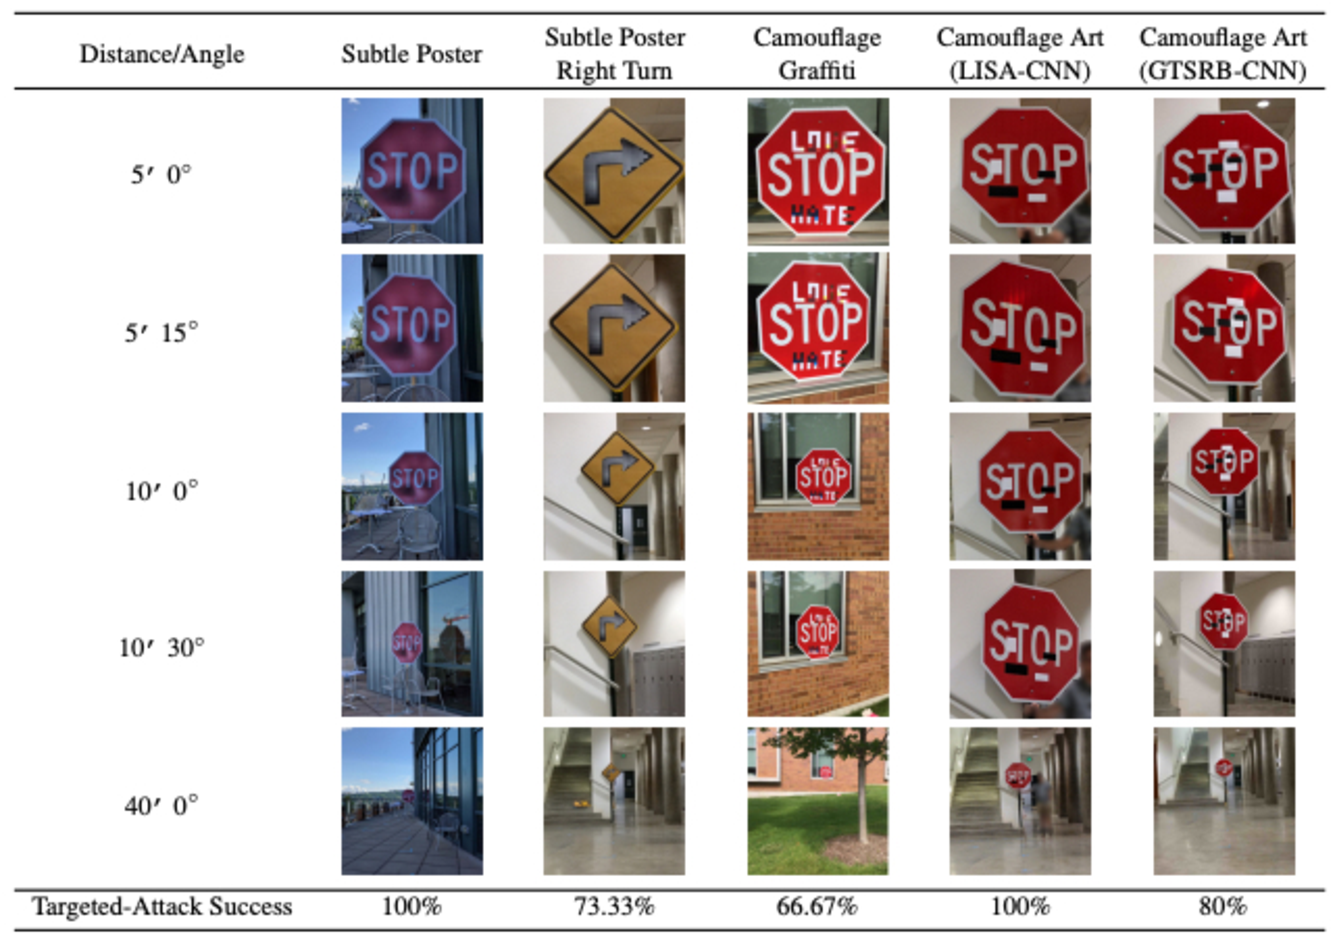
\includegraphics[width=14.0cm]{figures/robust-physical-result-image.pdf}
\end{center}
\caption{
距離と角度を変えて全 15 パターンを撮影してモデルに対する攻撃成功率を調べた結果.
画像はそのうちの 5 パターンを表示している.
Subtle Poster は摂動部分を含む画像全体を印刷したものであり, Camouflage は摂動部分のみを切り出し実際の標識に貼り付けたものになっている.
左から 2 列目と 3 列目は, mask をする部分を変更することで特定の位置にのみ摂動を加えている.
図は \cite{eykholt2018robust} より引用.
}
\label{fig:robust-physical-result-image}
\end{figure}
%

2 つめの実験の結果は図 \ref{fig:robust-physical-result-video} であり, 動画から切り出した画像に対しても摂動が有効に機能していることを示している.
標識部分を手動で crop して実験している点など実際の自動運転システムを攻撃するという観点からはまだまだ非現実的な点もあるが, digital な攻撃に比べれば現実的な physical attack の実現には大きく近づいていることが分かる.
%
\begin{figure}[htbp]
\begin{center}
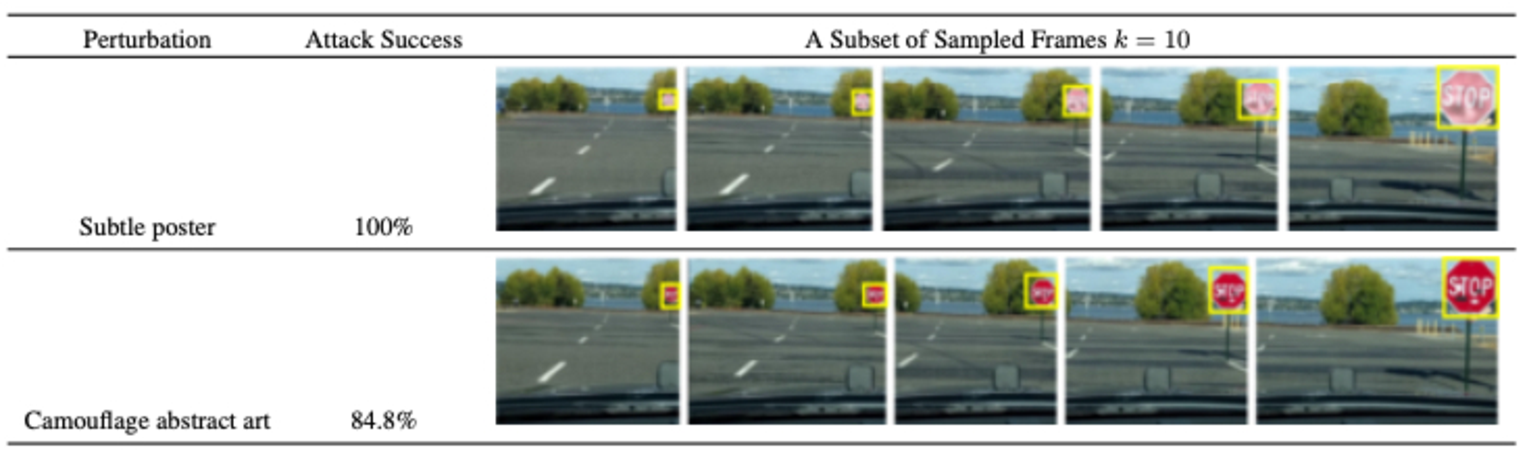
\includegraphics[width=15.0cm]{figures/robust-physical-result-video.pdf}
\end{center}
\caption{
実際に走行する車からスマートフォンで撮影した動画を 10 フレーム毎に切り出して標識部分を crop して, モデルに分類をさせて攻撃成功率を測定した結果.
図は \cite{eykholt2018robust} より引用.
}
\label{fig:robust-physical-result-video}
\end{figure}
%

この手法は検証実験のデータ量という点では不十分だが, digital な攻撃から physical な攻撃の実現可能性を高めたという点で注目に値すべきものである.
adversarial examples を作る根本的な方針自体は FGSM のようなシンプルなものからそう離れてはいないが, 距離や角度や輝度のような撮影環境が異なる場合にも攻撃成功率が高くなるように,  mask を作成して対象物のみに摂動を加えているという点が新しい.
これは以降の研究でもたびたび用いられることになる.



\subsection{One Pixel Attack for Fooling Deep Neural Networks}
\label{subsec:one-pixel}
%
\begin{table}[htbp]
\begin{center}
\begin{tabular}{|c|c|}
\hline
分類の観点 & この手法が該当するもの \\
\hline
Digital $\lor$ Physical & Digital \\
Classifier $\lor$ Detector & Classifier \\
摂動作成時に使用するデータ & 攻撃対象データ \\
摂動の加え方 & 画像全体 (ただし数ピクセルのみ) \\
知覚しづらさの定義 & 変更したピクセル数 \\
White box $\lor$ Black box & Black box \\
\hline
\multicolumn{2}{|c|}{非公式実装: \href{https://github.com/Hyperparticle/one-pixel-attack-keras}{https://github.com/Hyperparticle/one-pixel-attack-keras}} \\
\hline
\end{tabular}
\label{tb:one-pixel-summary}
\end{center}
\end{table}
%

これは \cite{su2019one} によって提案された手法であり, 差分進化アルゴリズムを用いて少数ピクセル (典型的には 1 $\sim$ 5 ピクセル) のみを変更することで誤認識させることに成功している.

この手法の特徴はモデルの勾配情報を用いない black box な攻撃であることと, 摂動として数ピクセルのみを対象としていることである.
変更されたピクセル数を知覚しづらさとして定義することができるが, これは同じ 1 ピクセルのみの変更でも人間にとって違いが明白な場合と不明瞭な場合がある.

使用しているアルゴリズムの本質的な部分は, 入力データの $i$ 成分を $x_i$ として, 世代 $g$ における値を以下のように決めることである.
%
\begin{eqnarray}
x_i (g + 1) = x_{r1} (g) + 0.5 (x_{r2} (g) - x_{r3} (g)) \ \ \text{where} \ \ r1 \neq r2 \neq r3.
\label{eq:de}
\end{eqnarray}
%
ここで, $r1, r2, r3$ は $i$ と同じ値の範囲を取る乱数である.
まず初期値としてランダムに 400 個の $x(g=0)$ を作成し, 差分進化アルゴリズム \ref{eq:de} を用いて新たに 400 個の $x(g=1)$ を作成して $x(g=0)$ と比べてモデルの softmax 値の意味で攻撃が成功に近づく方を残す.
特定のラベルに誤認識させたい場合は $y_{\text{atk-tge}}$ を設定してそれに対応する softmax 値が高くなるようにして, 特定のラベルを設定しない場合は $y_{\text{true}}$ に対応する softmax 値が小さくなるようにする.
$y_{\text{atk-tge}}$ を設定する場合は 90\% 以上になるか, 設定しない場合は 5\% 以下になるか, 世代が 100 になるまで進化を繰り返す.

kaggle CIFAR10 (\href{https://www.kaggle.com/c/cifar-10/data}{https://www.kaggle.com/c/cifar-10/data}) をデータとして用いる場合, 使用モデルは convolution のみで構成した AllConv と NIN \cite{lin2013network} と VGG16 である.
adversarial examples の作成に時間を要するため, CIFAR10 ではテストデータから 500 件ランダムにサンプリングして検証している.
ILSVRC2012 をデータとして用いる場合, 使用モデルは AlexNet である.
ILSVRC2012 ではテストデータから 105 件ランダムにサンプリングして検証している.

特徴的な結果は図 \ref{fig:one-pixel-example} のようになっており, 画像中の 1 ピクセルを変更するだけで特定のクラスに誤認識させることができていることが分かる.
%
\begin{figure}[htbp]
\begin{center}
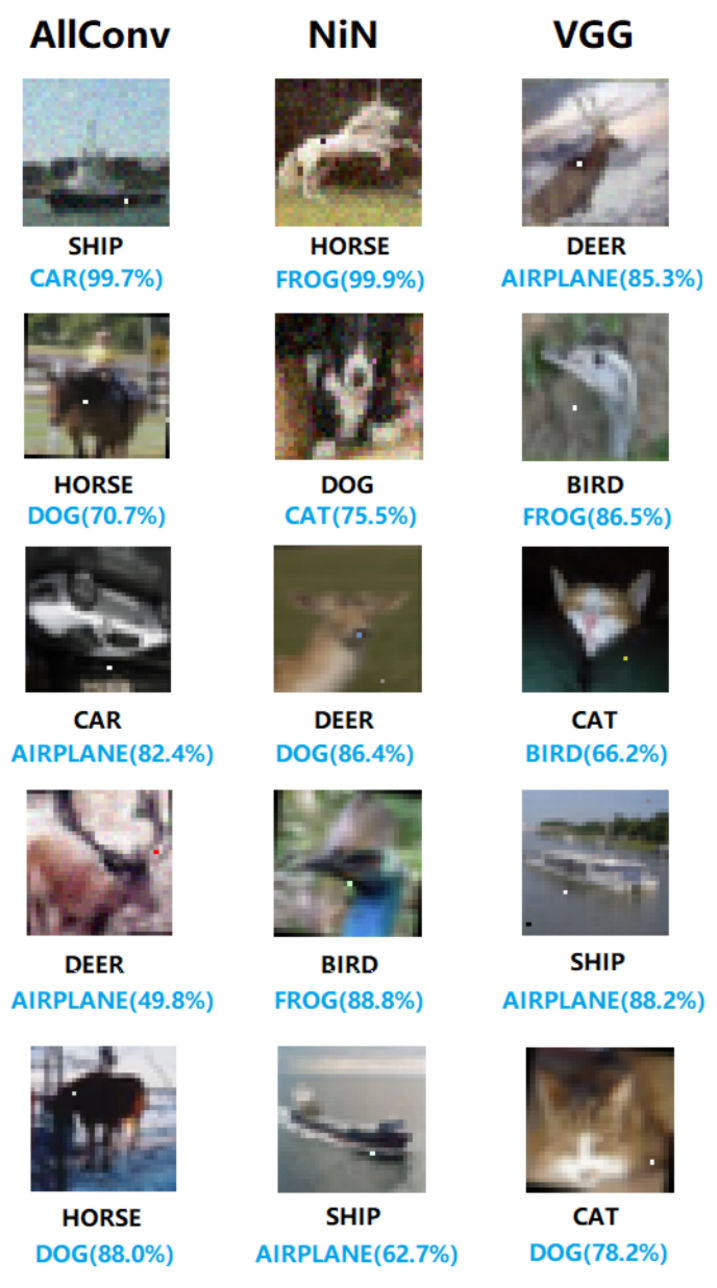
\includegraphics[width=8.0cm]{figures/one-pixel-example.pdf}
\end{center}
\caption{
kaggle CIFAR10 データに対して作成した adversarial examples の例.
黒字のクラスは $y_{\text{true}}$ で青字のクラスが $y_{\text{atk-tgt}}$ であり, どの画像も $y_{\text{atk-tgt}}$ クラスと予測されている.
図は \cite{su2019one} より引用.
}
\label{fig:one-pixel-example}
\end{figure}
%

CIFAR10 に対する adversarial examples は 1 ピクセルの変更でも人間にとって知覚しやすい.
これは画像サイズが小さいために変更箇所が顕著になるためで, ILSVRC2012 に対する adversarial examples は図 \ref{fig:one-pixel-imagenet} が示すように認識するのが難しい.
%
\begin{figure}[htbp]
\begin{center}
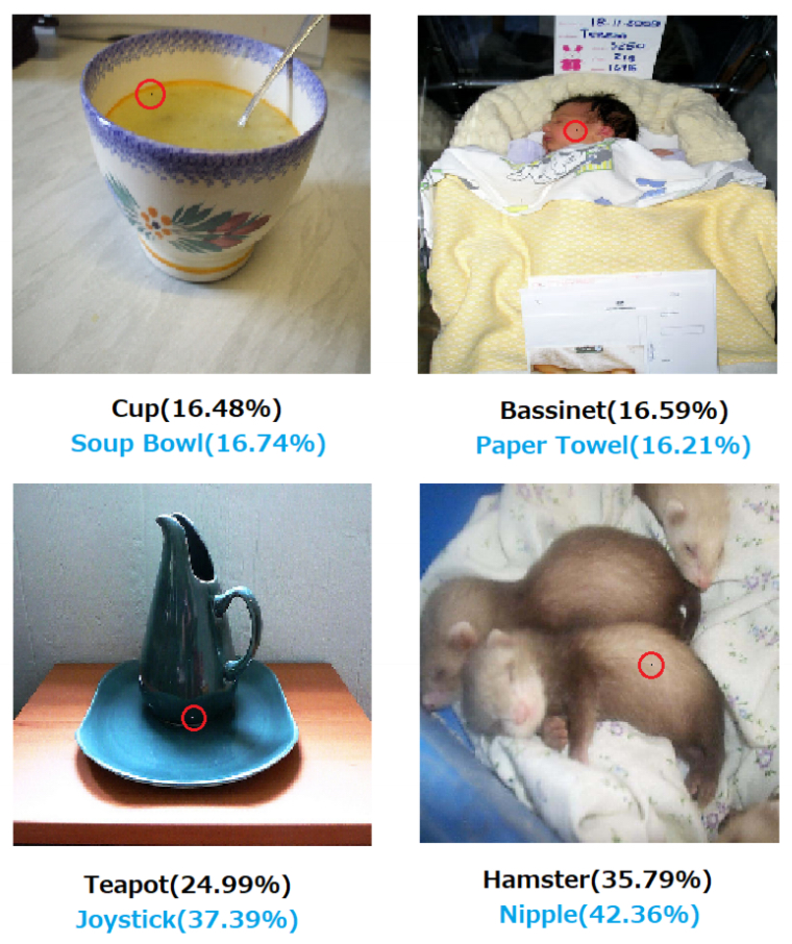
\includegraphics[width=8.0cm]{figures/one-pixel-imagenet.pdf}
\end{center}
\caption{
AlexNet モデルで ILSVRC2012 データに対して作成した adversarial examples の例.
黒字のクラスは $y_{\text{true}}$ で青字のクラスが $y_{\text{atk-tgt}}$ であり, どの画像も $y_{\text{atk-tgt}}$ クラスと予測されている.
赤い丸は変更したピクセルを視認しやすくするために後から付与した目印である.
図は \cite{su2019one} より引用.
}
\label{fig:one-pixel-imagenet}
\end{figure}
%

攻撃性能を調べた結果が図 \ref{fig:one-pixel-table} である.
Targeted ($y_{\text{atk-tgt}}$ を設定する場合) に比べると, Non-targeted ($y_{\text{atk-tgt}}$ を設定しない場合) はどのクラスに間違えさせても攻撃成功となるため誤認識率は上がっている.
ILSVRC2012 のように画像サイズが大きい場合でも成果ラベルうち 16\% を誤認識させることができている.
%
\begin{figure}[htbp]
\begin{center}
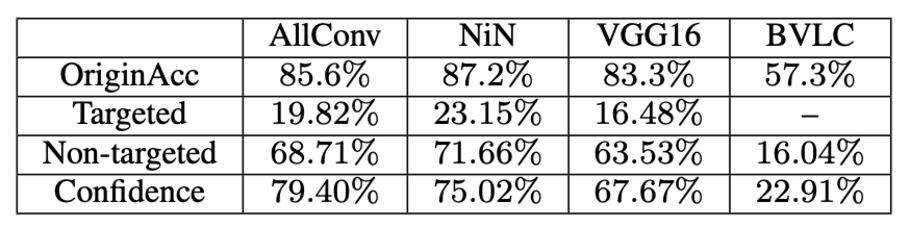
\includegraphics[width=10.0cm]{figures/one-pixel-table.pdf}
\end{center}
\caption{
1 ピクセルの変更による adversarial examples を作成して誤認識率を調べた結果.
OriginalAcc は clean データに対する正答率で, Targeted と Non-targeted は誤認識率を表している.
Confidence はモデルの softmax 値の最大の要素を平均した結果である.
モデルの BVLC は AlexNet を指している.
AllConv, NIN, VGG16 に関しては CIFAR10 を用いて, BVLC に関しては ILSVRC2012 を用いている.
Targeted の結果は正解以外の 9 クラスの結果を平均して算出しており, ILSVRC2012 の場合は計算量が多くなるため実施していない.
図は \cite{su2019one} より引用.
}
\label{fig:one-pixel-table}
\end{figure}
%

論文では変更するピクセル数を 3 ピクセルや 5 ピクセルに増やすことによる攻撃性能の向上や, 単なるランダム探索と比べて差分進化の有効性を示したりもしているが, ここでは割愛する.

この手法は摂動を加えるのが数ピクセルであっても DNN を誤認識させることができるという興味深い結果であったため注目を集めた.
攻撃成功率はそこまで高くはないが, ILSVRC2012 のように数百 $\times$ 数百ピクセルという画像においても有効であり, 人間ではほとんど気付かない adversarial examples を作成し得る.
また, DNN の予測がいかに不安定なものであるかを改めて認識させるものであった.



\subsection{Generating Natural Adversarial Examples}
\label{subsec:generating-natual}

\begin{table}[htbp]
\begin{center}
\begin{tabular}{|c|c|}
\hline
分類の観点 & この手法が該当するもの \\
\hline
Digital $\lor$ Physical & Digital \\
Classifier $\lor$ Detector & Classifier \\
摂動作成時に使用するデータ & 学習データと攻撃対象データ \\
摂動の加え方 & GANで画像を生成 \\
知覚しづらさの定義 & 潜在空間での $l_2$ \\
White box $\lor$ Black box & Black box \\
\hline
\multicolumn{2}{|c|}{公式実装: \href{https://github.com/zhengliz/natural-adversary}{https://github.com/zhengliz/natural-adversary}} \\
\hline
\end{tabular}
\label{tb:generating-natual-summary}
\end{center}
\end{table}

これは \cite{zhao2017generating} によって提案された手法であり, adversarial examples 作成の概要は図 \ref{fig:generating-natural-summary} のようになっている.
入力データ $x$ を inverter を用いて潜在空間に写し, 潜在空間で摂動を加えてそれを generator で入力データと同じ空間に写すことで $x_{\text{adv}}$ を作成する.
このとき, generator で写した $x_{\text{adv}}$ が $f_{\text{label}} (x_{\text{adv}}) \neq f_{\text{label}} (x)$ となるように要請する.
入力データの空間ではなく潜在空間での摂動を考えることで, 入力データと意味的に近いが予測結果は異なるような自然な adversarial examples が作れると期待している.
また, この手法は画像データにもテキストデータにも適用することができる.
%
\begin{figure}[htbp]
\begin{center}
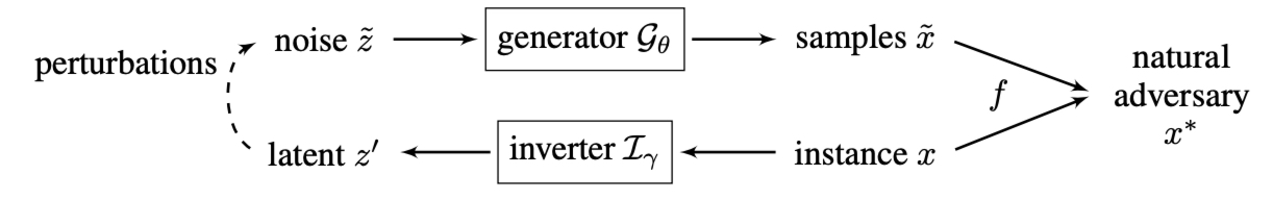
\includegraphics[width=14.0cm]{figures/generating-natural-summary.pdf}
\end{center}
\caption{
adversarial examples 作成の概要.
摂動は入力データの空間ではなく潜在空間で与える.
図は \cite{zhao2017generating} より引用.
}
\label{fig:generating-natural-summary}
\end{figure}
%

この手法は generator $\mathcal{G}_{\theta}$ と critic (discriminator) $\mathcal{C}_{\omega}$ から成る GAN の仕組みに加えて, inverter $\mathcal{I}_{\gamma}$ という入力データを潜在空間に写す三つ組から構成される.
学習の全体図は図 \ref{fig:generating-natural-training} のようになっている.
%
\begin{figure}[htbp]
\begin{center}
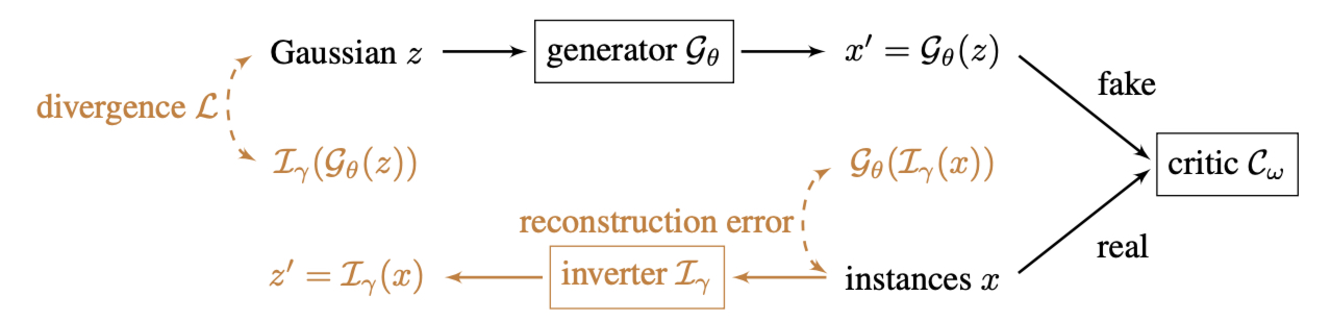
\includegraphics[width=14.0cm]{figures/generating-natural-training.pdf}
\end{center}
\caption{
generator, critic, inverter の三つ組の学習の全体図.
divergence $4\mathcal{L}$ は loss function $J$ に対応している.
図は \cite{zhao2017generating} より引用.
}
\label{fig:generating-natural-training}
\end{figure}
%
まず, generator と critic の学習は通常の GAN の枠組み通りで, Wasserstein-1 距離を用いて以下の min-max を解く.
%
\begin{eqnarray}
\min_{\theta} \max_{\omega} \left[ \mathbb{E}_{x \sim p_x (x)} \left[ \mathcal{C}_{\omega} (x) \right] - \mathbb{E}_{z \sim p_z (z)} \left[ \mathcal{C}_{\omega} (\mathcal{G}_{\theta} (z)) \right] \right].
\label{eq:gan-wasserstein}
\end{eqnarray}
%
この手法ではさらに inverter を次のように学習する.
%
\begin{eqnarray}
\min_{\gamma} \left[ \mathbb{E}_{x \sim p_x (x)} \| \mathcal{G}_{\theta} (\mathcal{I}_{\gamma} (x)) - x \| + \lambda \mathbb{E}_{z \sim p_z (z)} \left[ J(z, \mathcal{I}_{\gamma} (\mathcal{G}_{\theta} (z)) \right] \right].
\label{eq:inverter-training}
\end{eqnarray}
%
これは, 第一項は入力データを inverter で潜在空間に写してそれを generator で入力データの空間に戻した時に元の入力を再現するように要請しているもので, 第二項は潜在空間でのノイズを generator で入力データの空間に写してそれを inverter で戻したときに元のノイズを再現するように要請しているものである.
第二項は第一項の逆向きの流れを辿っているが, loss や扱うデータによって扱い方を変えている.
画像データの場合は loss function として $l_2$ ノルムを使い, $\lambda = 0.1$ としている.
学習自体は clean データのみを使用している.

学習した inverter と generator を用いて adversarial examples を作成する.
入力データ $x$ と攻撃対象のモデル $f_{\text{label}}$ があるとき, 入力データに潜在空間の $l_2$ の意味で近いが異なるラベルに予測されるような adversarial examples を作ることを目的としている.
これは以下のようにして実現される.
%
\begin{eqnarray}
x_{\text{adv}} = \mathcal{G}_{\theta} (z^*) \ \ \text{where} \ \ z^* = \argmin_{z'} \| z' - \mathcal{I}_{\gamma} (x) \| \ \text{s.t.} \ f_{\text{label}} (\mathcal{G}_{\theta} (z')) = f_{\text{label}} (x).
\label{eq:search-adversarial-example}
\end{eqnarray}
%
潜在空間でのノイズの加え方には指針がないため, 基本的にはランダム探索をする必要がある.
単に元の入力 $x$ を潜在空間に写した $z$ から近いところをランダムに探索して予測結果が変わるものを探すのは効率が悪いため, 論文では広い範囲を探索してからそれを二分探索で狭くしていくという方法を用いて 4 倍ほど高速化したと報告している.

実験としては MNIST と LSUN \cite{yu2015lsun} で実施している.
まず, MNIST で作成した adversarial examples と摂動部分を調べた例が図 \ref{fig:generating-natural-mnist} である.
FGSM で作成した摂動は画像全体に渡り, 3 という数字との関連の見えないものになっているが, 提案手法で作成した摂動は 3 という数字に合わせたものになっており, より元の入力データに意味的に近いが異なるモデル予測を導くものになっていることが見て取れる.
%
\begin{figure}[htbp]
\begin{center}
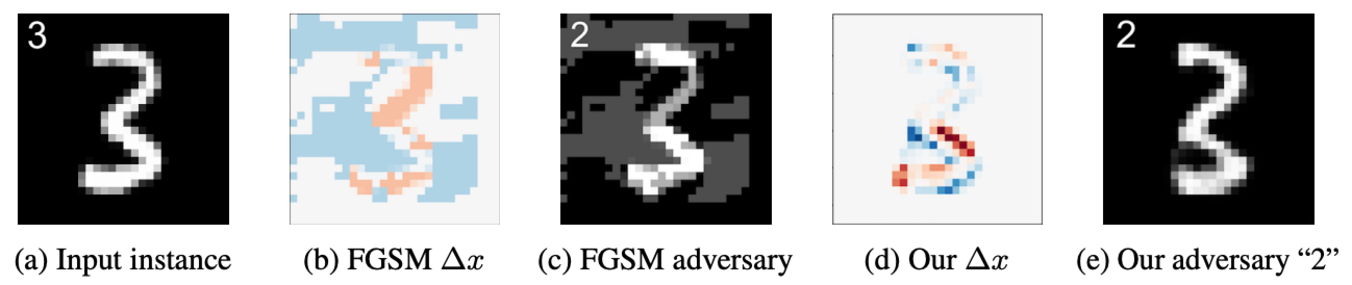
\includegraphics[width=14.0cm]{figures/generating-natural-mnist.pdf}
\end{center}
\caption{
MNIST で作成した摂動と adversarial examples の例.
$\Delta x$ は作成した摂動である.
図は \cite{zhao2017generating} より引用.
}
\label{fig:generating-natural-mnist}
\end{figure}
%

次に LSUN の結果が図 \ref{fig:generating-natural-example} である.
生成している画像なので不自然な画像にはなってしまっているが, 誤認識させたいラベルの雰囲気を似せるように変換されている様子が見て取れる.
%
\begin{figure}[htbp]
\begin{center}
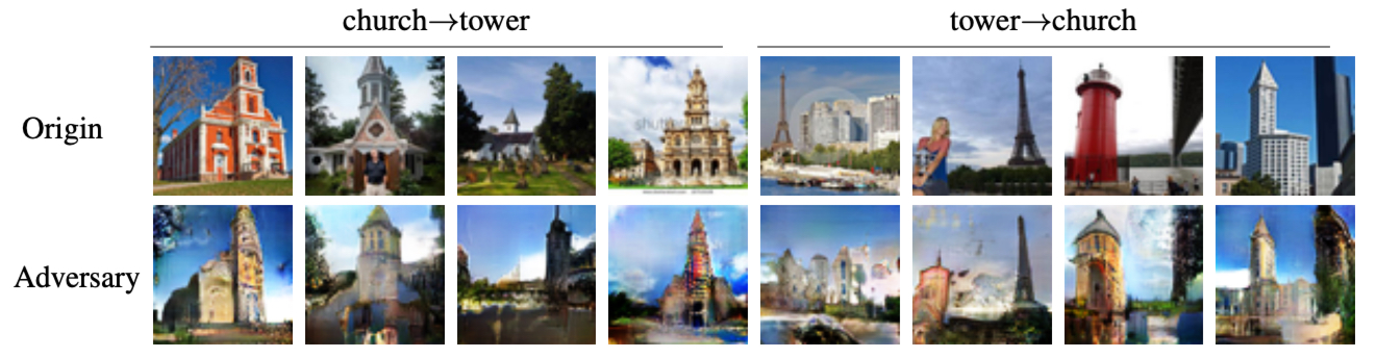
\includegraphics[width=14.0cm]{figures/generating-natural-example.pdf}
\end{center}
\caption{
LSUN で作成した adversarial examples の例.
元のラベルが {\it church} と {\it tower} のものをもう一方のものに誤認識させる adversarial examples になっている.
図は \cite{zhao2017generating} より引用.
}
\label{fig:generating-natural-example}
\end{figure}
%

どのくらいこの手法の攻撃が効率的なのかという観点で潜在空間での $z$ と $z^*$ の $l_2$ 距離の平均などを計測しているが, これらにそれほど意味は感じられないため割愛する.
また, この論文では入力データ空間での差分は気にしておらず, それは generator で生成される画像が見た目が元の入力データから離れていたとしても自然であると仮定しているためである (が, 例で見たようにこの時点での generator ではそれほど自然な画像は生成できていない).

この手法の興味深い点は入力データ空間ではなく潜在空間で摂動を加えるという点にある.
発表当時の GAN のレベルでは複雑なデータに対して十分自然な画像を生成することは難しかったが, 現在の発展に基づきより自然な画像で誤認識を引き起こすものを生成してみるのは面白いかもしれない.



\subsection{Beyond Pixel Norm-Balls: Parametric Adversaries using an Analytically Differentiable Renderer}
\label{subsec:beyond-pixel}
%
\begin{table}[htbp]
\begin{center}
\begin{tabular}{|c|c|}
\hline
分類の観点 & この手法が該当するもの \\
\hline
Digital $\lor$ Physical & Digital (防御は Physical) \\
Classifier $\lor$ Detector & Classifier \\
摂動作成時に使用するデータ & 3D object データ \\
摂動の加え方 & 対象物のみ \\
知覚しづらさの定義 & 色味が変わるなどの定性的評価 \\
White box $\lor$ Black box & White box \\
\hline
\multicolumn{2}{|c|}{実装なし (著者にメールしたが返信なし)} \\
\hline
\end{tabular}
\label{tb:beyond-pixel-summary}
\end{center}
\end{table}
%

これは \cite{liu2018beyond} によって提案された手法であり, 3D object データと微分可能レンダラーを用いて対象物の形状に沿った摂動を加えることで実現する色味や形状の変化で誤認識を引き起こす.

この手法を理解するためにはレンダリングの基礎知識が必要となるが, ここでは既知のものとして割愛する\footnote{
概念のみを述べておくと, レンダリングとは光学系をシミュレートして 3D 情報から 2D 画像を生成することである.
原論文の Appendix B に簡単な解説が書いてあるので, 興味があれば読んでみるのがよいだろう.
微分可能レンダラーはレンダラー部分も DNN で表現することで微分可能な構造を提供し, 誤差の伝播などを扱いやすくしたレンダラーである.
}.
レンダラーと 3D オブジェクトの情報があれば, まず対象となるオブジェクトに対してのみ適用される摂動を作成することができる.
そしてそれが 2D 画像に投影することができるため, 対象オブジェクトのみに摂動が加えられた adversarial examples が作成できる.
この論文では対象オブジェクトに加える摂動として lighting ($U$) と geometry ($V$) なるものを考案している.
例としては図 \ref{fig:beyond-pixel-example} のようなものとなる.
提案手法が物体形状に沿った自然な摂動になっていることが見て取れる.
%
\begin{figure}[htbp]
\begin{center}
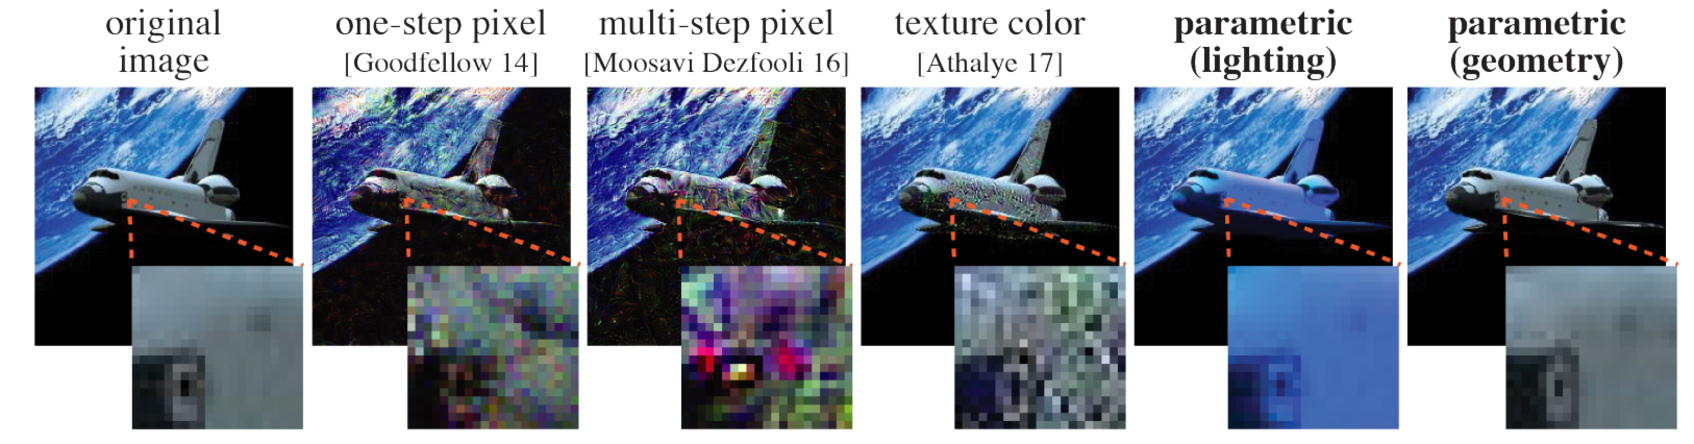
\includegraphics[width=14.0cm]{figures/beyond-pixel-example.pdf}
\end{center}
\caption{
提案手法による摂動の例.
まず, 各画像は 2D の背景画像の上に 3D の飛行機のオブジェクトをレンダリングして 2D 画像を作成している.
攻撃方法の左 2 つは作成した 2D 画像に対して摂動を加えるため摂動は画像全体に広がっている.
texture color はオブジェクトのみに摂動を加える先行研究で, 3D オブジェクトに対して摂動を作成してそれを 2D にレンダリングしているので飛行機のみに摂動が加えられているが, 不自然な摂動となっていて人間が気付きやすい.
右 2 つの提案手法も摂動を 3D オブジェクトに対して作成してからレンダリングしているが, 色味やわずかな形状を変えるのみで自然な摂動になっている.
図は \cite{liu2018beyond} より引用.
}
\label{fig:beyond-pixel-example}
\end{figure}
%

微分可能レンダラー \cite{kato2018neural} を用いることで, 2D 画像に対する loss を逆伝播して 3D オブジェクトに反映させることが可能となる.
つまり, 3D オブジェクトからスタートして, それを微分可能レンダラーに通して 2D 画像を作成し, 予測モデルでその 2D 画像に対する loss を計算する, を逆向きに辿っていって予測モデルが誤認識する摂動を 3D オブジェクトに加えることができる.
摂動として自然なものを作成するため, この論文では 3D オブジェクトのパラメタを用いて lighting ($U$) と geometry ($V$) を定義する.
これらは低次の球面調和関数の係数や 3D オブジェクトを三角分割した際の法線や頂点などで記述されるが, ここでは詳細を割愛する.
微分可能レンダラーを介して 2D 画像 $I$ を $I(U, V)$ と書くことができるため (微分可能レンダラーのパラメタは陽には書いていない), 以下のように loss を微分した量が計算できれば勾配法で摂動が作成できる.
%
\begin{eqnarray}
\frac{\partial J}{\partial U} &=& \frac{\partial J}{\partial I} \frac{\partial I}{\partial U}.\\
\frac{\partial J}{\partial V} &=& \frac{\partial J}{\partial I} \frac{\partial I}{\partial V}.
\label{eq:beyond-pixel-diff}
\end{eqnarray}
%
それぞれ右辺の第一項は loss function を 2D 画像で微分しているのみなので特に難しいところはない.
第二項は 2D の画像を 3D オブジェクトのパラメタで微分するため, 微分可能レンダラーを介して計算される量である.

具体的な表式を割愛すれば, 手法としては以上である.
lighting を変えた誤認識させる例は図 \ref{fig:beyond-pixel-lighting} である.
対象物の色味が変わっているだけなので, 摂動としては不自然さは少ない (3D オブジェクトをレンダリングして作成しているので背景画像とのミスマッチ感はある).
%
\begin{figure}[htbp]
\begin{center}
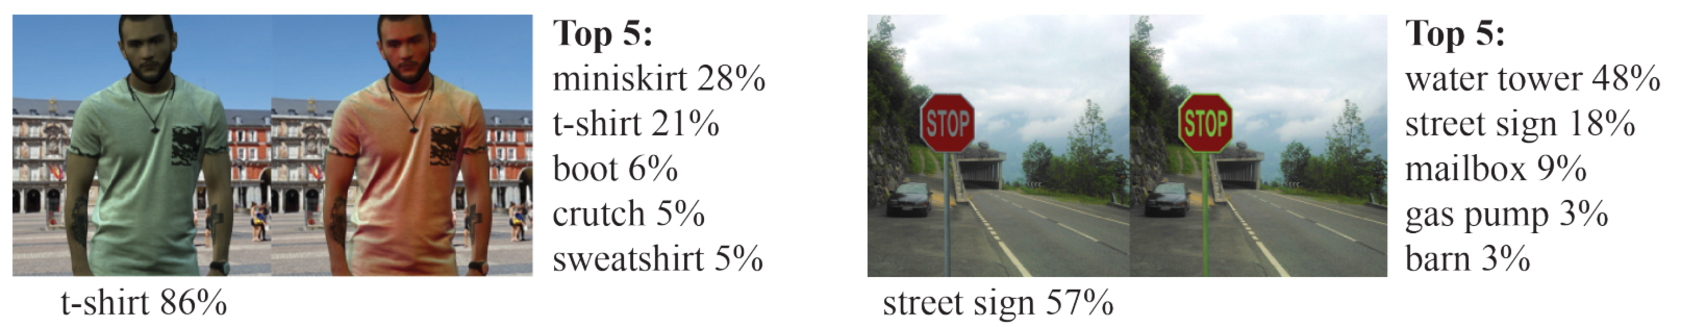
\includegraphics[width=14.0cm]{figures/beyond-pixel-lighting.pdf}
\end{center}
\caption{
lighting を変えて作成した adversarial examples の例.
背景の 2D 画像に lighting を変えた 3D オブジェクトをレンダリングして最終的な 2D 画像を作成している.
モデルによる予測は ILSVRC2012 で pre-train された ResNet-101 で実施している.
図は \cite{liu2018beyond} より引用.
}
\label{fig:beyond-pixel-lighting}
\end{figure}
%

3D オブジェクトに対する手法であるため, 様々に角度を変えても同じように誤認識させる摂動を作成することもできる.
それを示したのが図 \ref{fig:beyond-pixel-diff-angle} であり, 異なる角度に対してもモデルが同様に誤認識している様子が見て取れる.
%
\begin{figure}[htbp]
\begin{center}
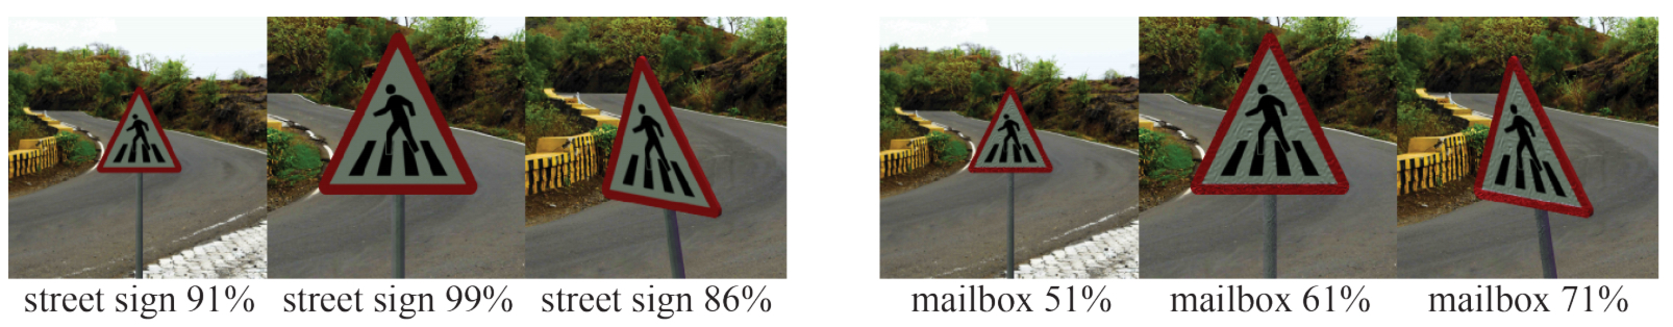
\includegraphics[width=14.0cm]{figures/beyond-pixel-diff-angle.pdf}
\end{center}
\caption{
角度を変えても同様に誤認識をさせることに成功している例.
摂動は geometry に対して作成している.
背景の 2D 画像に lighting を変えた 3D オブジェクトをレンダリングして最終的な 2D 画像を作成している.
モデルによる予測は ILSVRC2012 で pre-train された ResNet-101 で実施している.
図は \cite{liu2018beyond} より引用.
}
\label{fig:beyond-pixel-diff-angle}
\end{figure}
%

提案手法による摂動は対象物のみに加える摂動で対象物の光学的・幾何学的変換に基づくものであるため, より対象物そのものの性質を捉えたもので adversarial examples として transferability も高い.
ResNet で作成した 5,000 枚の adversarial examples を他のモデルで検証した結果が図 \ref{fig:beyond-pixel-transferability} で, 多くのモデルが高い確率で誤認識している.
%
\begin{figure}[htbp]
\begin{center}
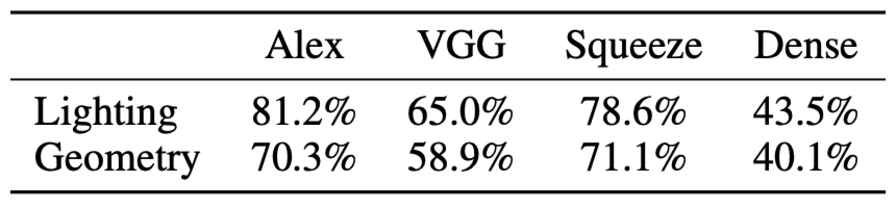
\includegraphics[width=8.0cm]{figures/beyond-pixel-transferability.pdf}
\end{center}
\caption{
ResNet で作成した 5,000 枚の adversarial examples に対する他のモデルの誤認識率 (1 - 正答率).
モデルは AlexNet, VGG, SqueezeNet \cite{iandola2016squeezenet}, DenseNet \cite{huang2017densely} を用いている.
図は \cite{liu2018beyond} より引用.
}
\label{fig:beyond-pixel-transferability}
\end{figure}
%

この手法は微分可能レンダラーを用いて 3D オブジェクトに対して摂動を作成してそれを 2D に写すという点が興味深い.
より対象物に特化した摂動を作成することが可能になっている.
必要となる道具が多いのと 3D オブジェクトデータも必要になる手法ではあるが, \cite{athalye2017synthesizing} のように 3D プリンターで作成した adversarial examples も登場しているため, 一つの面白い方向性だろう.



\subsection{On the Structural Sensitivity of Deep Convolutional Networks to the Directions of Fourier Basis Functions}
\label{subsec:on-the}
%
\begin{table}[htbp]
\begin{center}
\begin{tabular}{|c|c|}
\hline
分類の観点 & この手法が該当するもの \\
\hline
Digital $\lor$ Physical & Digital \\
Classifier $\lor$ Detector & Classifier \\
摂動作成時に使用するデータ & 学習データ \\
摂動の加え方 & 画像全体 \\
知覚しづらさの定義 & $l_{\infty}$ \\
White box $\lor$ Black box & Black box  (出力ラベルのみ) \\
\hline
\multicolumn{2}{|c|}{実装なし} \\
\hline
\end{tabular}
\label{tb:on-the-summary}
\end{center}
\end{table}
%

これは \cite{tsuzuku2019structural} によって提案された手法であり, 周波数領域でフーリエ基底を用いてデータに依らない adversarial examples を作成する.
DNN は adversarial examples に対して線形分類器に近い振る舞いをするという経験的事実と, CNN が周波数領域で特徴量を学習しているという経験的事実を合わせて, 周波数領域で摂動を構成することでデータに依らずに様々な CNN に対して有効な adversarial examples の作成を実現している. 
adversarial examples 作成時にモデルの出力ラベルのみを用いる真の black box attack となっている点も特徴である.

道具としてフーリエ基底や離散フーリエ変換が必要となるため, 簡単に復習する.
虚数の N 乗根を $s_N = \exp (2 \pi i / N)$ として, $s_N^{u,v} = s_N^u s_N^v \in \mathcal{C}^{N \times N}$ とする.
これを用いて以下の $N \times N$ 行列を定義する.
%
\begin{eqnarray}
(F_N)_{u,v} = \frac{1}{\sqrt{N}} s_N^{u, v}.
\label{eq:on-the-matrix}
\end{eqnarray}
%
座標領域から波数領域への離散フーリエ変換は以下のように書ける.
%
\begin{eqnarray}
S(x)_{u,v} = \sum_{m=0}^{N-1} \sum_{n=0}^{N-1} x_{m,n} \exp (- 2 \pi i (u m + v n) / N)
\label{eq:on-the-dft}
\end{eqnarray}
%
これらは単なる定義である.
二次元 $N \times N$ を考えているのは画像が二次元空間 (height, width) であることに対応している (チャンネルの次元もあるがこれらは波数を求める対象ではない).
また, 導入した $s^{u,v}$ の添字は (height, width) の波数のモードと対応していて, これらの値が大きいほど波数が大きなモードとなっていることが分かる.

導入した $F_N$ を用いた $Q_N = \frac{1}{N} F_N \otimes F_N$ ($\otimes$ はクロネッカー積) が解析において重要な量となる.
これがなぜ重要なのかを詳しく知りたい場合は \cite{sedghi2018singular} も併せて読んでもらうとして, ここでは概略だけを述べる.
重要な点はチャンネル数が 1 の 2d-convolution の padding を wrap around\footnote{
各エッジでトーラス状につながるように padding するもの.
解析のしやすさのために用いている方法で実際にはあまり用いられることはない.
}
にする場合, doubly block circulant matrix $A$ を用いて 2d-convolution の演算が $\text{vec} (x_{\text{next}}) = A \cdot \text{vec} (x)$ のように書けるという点である.
詳細な定義は文献を追ってもらうとして, wrap around のような周期性がある padding であれば数学的には特徴的な行列で表現できることは想像に難くない.
そして, この 2d-convolution の情報を持つ行列 $A$ の固有値や固有ベクトルと深く関わっているのが $Q_N = \frac{1}{N} F_N \otimes F_N$ なのである.
具体的には, 例えば $A$ の固有ベクトルは $Q_N$ の列であることが示されている.

この事実を受け入れると, $Q_N$ がユニタリであること (これは定義より自明) から $A$ は複素対角行列 $D$ を用いて $A = Q_N D Q_N^{\dagger}$ ($Q_N^{\dagger}$ は $Q_N$ のエルミート共役) と分解できる.
これは左から $Q_N^{\dagger}$, 右から $Q_N$ を掛けることで簡単に固有値が求められることを意味する.
したがって, convolution の固有値や固有ベクトルが簡単に求まるため, 特定のモードの固有ベクトルだけを取り出して摂動を作成するということが実現できる.
そのような摂動が有効かどうかはここでの数学的な議論とは別物であるが, それを期待するには十分な経験的知識があり, 試してみたら上手く機能したというストーリーになっている.

ここでの議論はチャンネル数が 1 で convolution を 1 回だけ適用してかつ線形な activation のみに有効なものであるが, 論文ではチャンネル数を増やしたり convolution を stack したり skip connection を加えても同様の議論が成り立つことを証明している.
非線形な activation を考えると数学的な保証がなくなってしまうが, ReLU のように線形な activation からそう遠く離れてない場合はある程度上手くいくことが期待でき, それは実験的にも示される.

具体的に adversarial examples を作成するアルゴリズムは次のようになる.
$(F_N)_u$ を $u$ 番目の行のベクトルとして, ある入力画像 $x$ とアルゴリズム \ref{alg:on-the-single-fourier-attack} で作成した $x_{\text{adv}}$ で予測ラベルが異なるような波数モード $u, v$ を brute force で探す.
学習データ全体に対して誤認識率が最も高くなる $u, v$ の組を探しており, 2 つの離散的な変数であるため力技で解くことができる.
%
\begin{algorithm}
\caption{Single Fourier attack のアルゴリズム}
\label{alg:on-the-single-fourier-attack}
\begin{algorithmic}[1]
    \State Input: 波数モード $u, v$, 摂動の大きさ $\epsilon$.
    \State Output: adversarial examples $x_{\text{adv}}$.
	\State adversarial examples を初期化: $x_{\text{adv}} \leftarrow x$.
	\For {各チャンネル $c$}
	\State $x_{\text{adv}} \leftarrow x_{\text{adv}} + \epsilon ( (1 + u) (F_N)_u \otimes (F_N)_v + (1 - u) (F_N)_{N - u} \otimes (F_N)_{N - v} )$.
	\State $x_{\text{adv}} \leftarrow \text{clip} (x_{\text{adv}},0,1)$.
	\EndFor
\end{algorithmic} 
\end{algorithm}
%

実験はデータとしては MNIST, fashion MNIST, SVHN, CIFAR10, CIFAR100 を用いている.
モデルは LeNet, VGG, WideResNet \cite{zagoruyko2016wide}, DenseNet を用いており, 理論解析時に要請した wrap around の padding や線形な activation は用いていない (それでも上手くいくと期待している).
画像を扱うため座標領域では実数値を取る必要があるため, $S(x)_{u,v} = S(x)^{\dagger}_{N - u, N - v}$ を満たすものだけが許容される.
この条件式は式 \ref{eq:on-the-dft} の両辺のエルミート共役を取り $x_{m,n}$ が実数値であることを要請すれば導出できる.
このような条件を満たす各 $u, v$ に関してランダムにミニバッチを選んで誤認識率を計算したものが図 \ref{fig:on-the-uvplane} である.
これはあらゆる場合でこの手法が有効であるわけでないことを示しているが, データやモデルによってこれだけ振る舞いが変わるという点は興味深い.
また, 例えば SVHN では低波数成分が強く効いていることが分かるが, CIFAR では高波数成分が効いていることが分かり, 単純に低波数成分が摂動にとって支配的でないことが示されている.
%
\begin{figure}[htbp]
\begin{center}
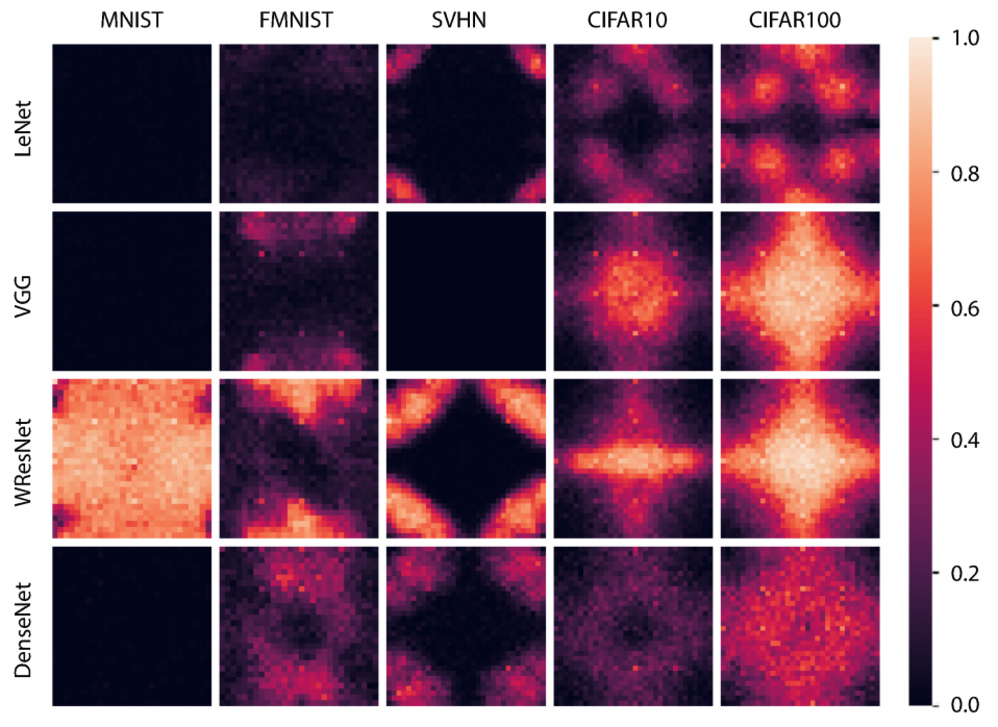
\includegraphics[width=12.0cm]{figures/on-the-uvplane.pdf}
\end{center}
\caption{
各データセット, 各モデルでの誤認識率 (1 - 正答率) を $(u, v)$ 平面でプロット結果.
色が白いところが誤認識率が高い領域である.
四隅が低波数領域で中心が高波数領域であり, これは離散フーリエ変換を考えれば $2 \pi$ が周期であるため, 例えば $u = v = N - 1$ の場合 exp の部分が $\exp (- 2 \pi i (m + n) / N)$ になり $u = v = 1$ と同じなることから理解できる.
図は \cite{tsuzuku2019structural} より引用.
}
\label{fig:on-the-uvplane}
\end{figure}
%

データセット全体に対する誤認識率を定量的に調べた結果が図 \ref{fig:on-the-fool-ratio} である.
シンプルな摂動でありながら大きく効果を発揮しているものが多い一方で, 先ほど見たように同じモデルでもデータによって全く摂動が効かないものも存在する.
また, 単純なノイズによっても WideResNet の誤認識が高くなったりもしていてモデルの構造依存性が大きいことが伺える.
%
\begin{figure}[htbp]
\begin{center}
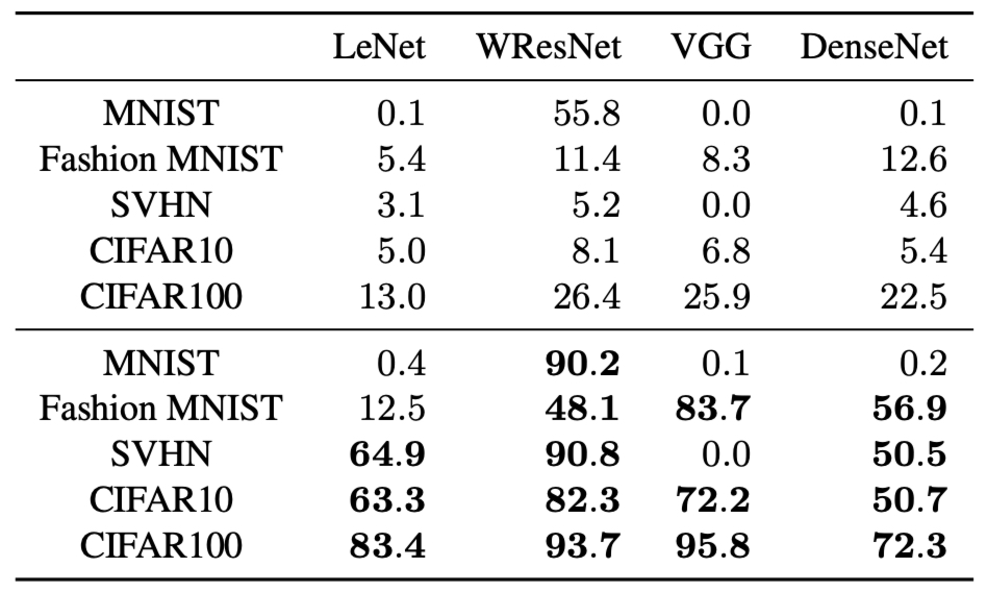
\includegraphics[width=10.0cm]{figures/on-the-fool-ratio.pdf}
\end{center}
\caption{
各データセットに対する各モデルの誤認識率 (1 - 正答率).
上段はデータにランダムなノイズを加えた結果で, 下段は Single Fourier Attack で作成した adversarial examples の結果.
図は \cite{tsuzuku2019structural} より引用.
}
\label{fig:on-the-fool-ratio}
\end{figure}
%

従来手法で作成し摂動を波数領域で調べるとどうなるのかは気になるところであるが, FGSM で作成した摂動を波数領域で調べた結果が図 \ref{fig:on-the-fgsm} である.
これは図 \ref{fig:on-the-uvplane} とは異なり誤認識率を表しているわけではなく, 作成した摂動がどの成分が大きいかを調べたものになっている.
具体的には FGSM で作成した摂動は各波数モードの線形和になっているため, 各モードに対応するベクトルの絶対値の平均を取っている.
波数で特徴付けられる摂動を作成していることが見て取れて, Single Fourier Attack の結果と同様に CIFAR では高波数モードも効いていることが分かる.
ただし, MLP のような単純なモデルではどのデータでも低波数モードのみが効いていることが分かり, シンプルな CNN では高波数成分を取り除くように重みが学習されて低波数成分が支配的であるということの一定の証拠となっている.
また, 例えば MNIST-VGG の組み合わせのように Single Fourier Attack では誤認識が確認できなかったものでも複数成分の重ね合わせをすれば誤認識させることができる.
これはフーリエ基底の一部だけで摂動を構築することの限界を示している.
%
\begin{figure}[htbp]
\begin{center}
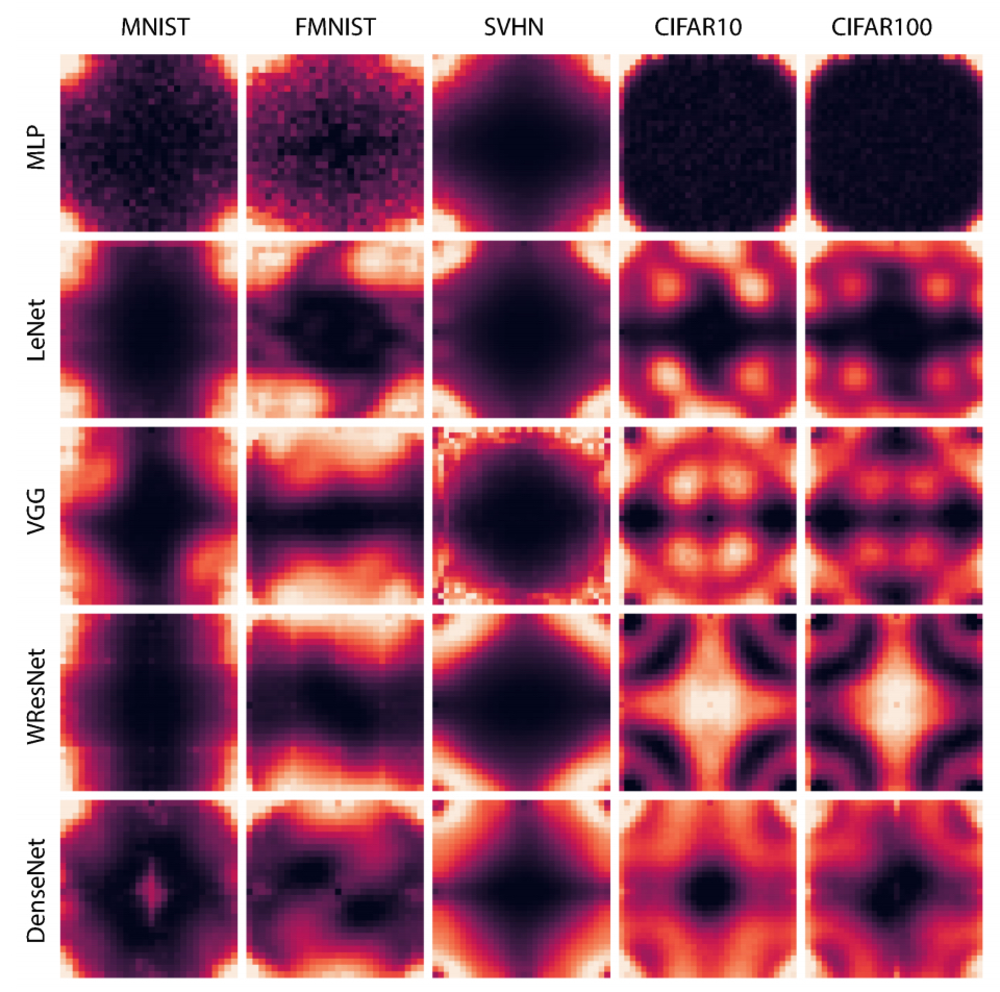
\includegraphics[width=10.0cm]{figures/on-the-fgsm.pdf}
\end{center}
\caption{
FGSM で作成した摂動の波数領域での大きさを調べたもの.
FGSM で作成した摂動は各波数モードの線形和であるため, 各モードに対応するベクトルの絶対値の平均を計算してプロットしている.
白色に近いほど値が大きい.
図は \cite{tsuzuku2019structural} より引用.
}
\label{fig:on-the-fgsm}
\end{figure}
%

この手法は CNN の固有値や固有ベクトルの解析と adversarial examples を組み合わせた点が興味深い.
理論的解析は padding として wrap around と線形な activation に限るものだが, 実際のモデルはそこから大きく外れるものではないので実験的にも作成した adversarial examples がうまく機能している.
データやモデル依存性が大きいため, このような方向性の議論を深めることでデータやモデルの特徴付けや分類が可能となるかもしれない.



\subsection{Adversarial camera stickers: A physical camera-based attack on deep learning systems}
\label{subsec:advdersarial-camera}
%
\begin{table}[htbp]
\begin{center}
\begin{tabular}{|c|c|}
\hline
分類の観点 & この手法が該当するもの \\
\hline
Digital $\lor$ Physical & Physical \\
Classifier $\lor$ Detector & Classifier \\
摂動作成時に使用するデータ & 攻撃対象データ \\
White box $\lor$ Black box & White box \\
摂動の加え方 & 画像全体 \\
知覚しづらさの定義 & ヒューリスティック \\
\hline
\multicolumn{2}{|c|}{非公式実装: \href{https://github.com/yoheikikuta/adversarial-camera-stickers}{https://github.com/yoheikikuta/adversarial-camera-stickers}} \\
\hline
\end{tabular}
\label{tb:advdersarial-camera-summary}
\end{center}
\end{table}
%

これは \cite{li2019adversarial} によって提案された手法であり, 作成した摂動をシールとして印刷してカメラのレンズに貼り付けることで攻撃対象の予測モデルの誤認識を引き起こす手法である.
従来手法が物体に摂動を加えることを考えていたのとは対照的に, カメラと物体間の光学的な path の間に操作を加えるという試みである.

摂動はカメラのレンズにシールを貼るだけで physical な環境で有効であるようなものにしたい.
少しずれたりしただけで効果が発揮されないような摂動では目的を達成できないため, あまり細かい摂動ではなくてぼやっとした摂動が適していると考えられ, この論文では色付き半透明の丸模様を複数個作成するという戦略を採用している.
具体的な数式は以下のようになる.
%
\begin{eqnarray}
(x_{\text{adv}})_{i,j} &=& (1 - \alpha_{i,j}) \cdot x_{i,j} + \alpha_{i,j} \cdot \gamma.
\label{eq:adversarial-camera-pi} \\
\alpha &=& \alpha_{\text{max}} \cdot \exp (- d^{\beta} (i,j)).
\label{eq:adversarial-camera-alpha} \\
d (i,j) &=& \frac{(i - i^{(\text{center})})^2 + (j - j^{(\text{center})})^2}{r^2}.
\label{eq:adversarial-camera-d}
\end{eqnarray}
%
ここで, $(i,j)$ は画像の二次元座標で, $\gamma \in [0, 1]^3$ で丸模様の色である.
この $x_{\text{adv}}$ ある中心 $(i^{(\text{center})}, j^{(\text{center})})$ から離れるほど指数的に薄くなる丸模様を元画像とアルファブレンディングしたものである.
この数式で表現される丸模様は一つだけだが, これを複数回適用することで実際の摂動を作成する.
あるクラス $y^{*}$ の画像 $M$ 個をまとめて $y_{\text{atk-tgt}}$ に間違えさせるという問題設定を考えていて, loss function は以下のように構成する.
%
\begin{eqnarray}
\sum_{m = 1}^{M} \left(- J(f, x_{\text{adv}}, y^*) + J(f, x_{\text{adv}}, y_{\text{atk-tgt}}) \right).
\label{eq:adversarial-camera-loss}
\end{eqnarray}
%

あとは式 \ref{eq:adversarial-camera-pi},\ref{eq:adversarial-camera-alpha},\ref{eq:adversarial-camera-d} で導入された各パラメタと丸模様の数に関してこの loss function が小さくなるように最適化して得られた結果をシールとして印刷すればよいが, パラメタが多いため最適化は容易ではない.
ヒューリスティックや予備実験によって, 丸模様の数を 10 個に固定して, $r, \alpha_{\text{max}}, \beta$ も固定し, $\gamma$ は 10 組 (その集合を $\Gamma$ とする) に限定した上で $\gamma$ とそれぞれの丸模様の中心位置について最適化を実施するという簡単化をしている.
この簡単化はかなり大変な作業で, まず物理的に実現可能, 知覚もしにくく, モデルを誤認識させることができるようなシールをヒューリスティックに作成する\footnote{
この辺りの詳細は書いてなく, 著者に聞いても詳しくは教えてくれなかったが大変だったと語っていた.
}.
このヒューリスティックに作成した摂動を再現するようなパラメタを SSIM \cite{wang2004image} を最大化するという条件で求めるというアプローチになっている.
固定したパラメタはこのようにして求めている.
残りの $\gamma$ とそれぞれの丸模様の中心位置の最適化はアルゴリズム \ref{alg:adversarial-camera-alg} で求める.
$\gamma$ は離散集合から選択するため勾配法が使えないので, まずは丸模様の中心位置も $45 \times 45$ のグリッドに離散化した状況下 ($\mathcal{C}$ と書く) での greedy な最適化を実施する.
$\gamma$ の値と大体の丸模様の中心位置が定まったら, 丸模様の中心位置は連続量に戻して勾配法で細かい調整をするという手順となる.
%
\begin{algorithm}
\caption{$\gamma$ と丸模様の中心位置を定めるアルゴリズム}
\label{alg:adversarial-camera-alg}
\begin{algorithmic}[1]
    \State Input: 丸模様の数 $K$, 攻撃対象のクラス $y^*$, ターゲットクラス $y_{\text{atk-tgt}}$, $y^*$ に属する画像 $x^{(1)}, \dots, x^{(M)}$.
    \State Output: 摂動を作成するための $\gamma_k$ と $(i^{(\text{center})}_k, j^{(\text{center})}_k)$.
	\State 摂動を初期化: $(i^{(\text{center})}_k, j^{(\text{center})}_k) \leftarrow \text{some values}$.
	\Repeat
	\For {各$k \in K$}
	\For {$(i^{(\text{center})}_k, j^{(\text{center})}_k), \gamma_k \in \mathcal{C} \times \Gamma$}
	\State 式 \ref{eq:adversarial-camera-loss} を評価.
	\EndFor
	\State loss が最小になる $(i^{(\text{center})}_k, j^{(\text{center})}_k), \gamma_k$ を選ぶ.
	\EndFor
	\Until {loss が収束するまで}
	\State
	\Repeat
	\For {$k \in K$}
	\State $(i^{(\text{center})}_k, j^{(\text{center})}_k)$ を式 \ref{eq:adversarial-camera-loss} の勾配を計算して勾配法で更新.
	\EndFor
	\Until {loss が収束するまで}
\end{algorithmic} 
\end{algorithm} 
%

最終的に作成した摂動とそれをカメラのレンズに貼って撮影した画像の例が図 \ref{fig:adversarial-camera-example} である.
どちらも誤認識させることができた画像を集めており, 様々な撮影条件において誤認識させることができていることに加え, 撮影された画像は少し汚れのように色がついているのが認識される程度である.
%
\begin{figure}[htbp]
\begin{center}
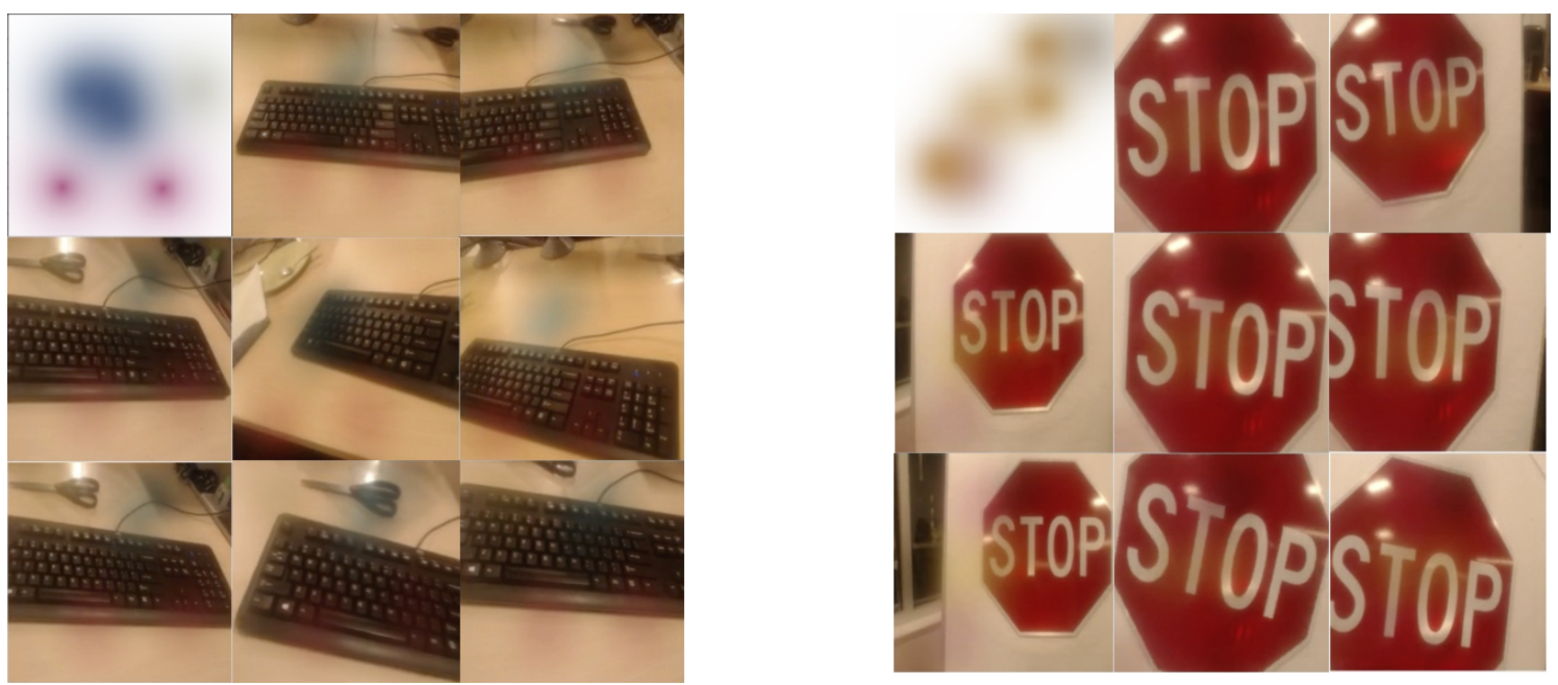
\includegraphics[width=12.0cm]{figures/adversarial-camera-example.pdf}
\end{center}
\caption{
作成した摂動とそれを印刷してカメラに貼って撮影した画像の例.
左側は {\it computer keyboard} クラスを {\it mouse} クラスに誤認識させていて, 右側は {\it street sign} クラスを {\it guitar pick} クラスに誤認識させている.
モデルは ILSVRC2012 pre-trained の ResNet-50 を用いている.
図は \cite{li2019adversarial} より引用.
}
\label{fig:adversarial-camera-example}
\end{figure}
%

作成した摂動の性能を定量的に測るため, 動画を 1,000 フレーム撮影してそれぞれを ILSVRC2012 pre-trained の ResNet-50 で予測した結果が図 \ref{fig:adversarial-camera-fool-ratio} である.
誤認識させることができたフレーム数は半分程度ではあるが, 確かに作成した摂動が有効に機能していることが示されている.
%
\begin{figure}[htbp]
\begin{center}
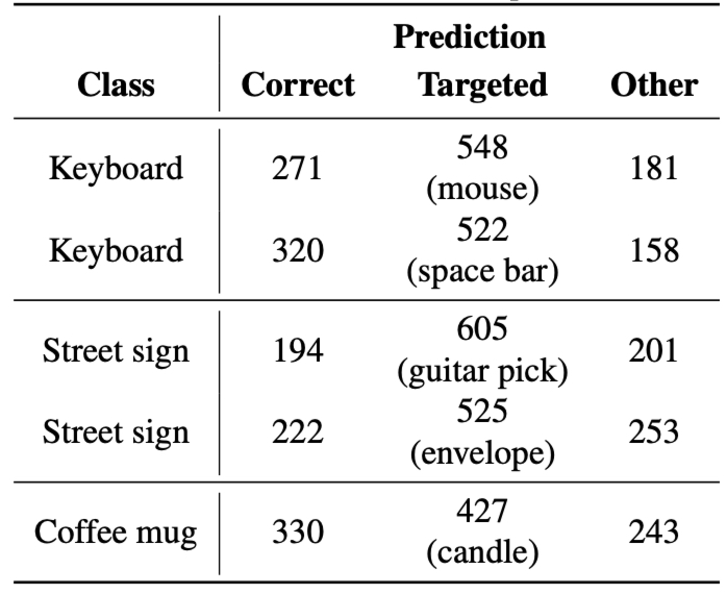
\includegraphics[width=6.0cm]{figures/adversarial-camera-fool-ratio.pdf}
\end{center}
\caption{
作成した摂動とそれを印刷してカメラに貼って動画を 1,000 フレーム撮影し, ILSVRC2012 pre-trained の ResNet-50 で予測させた結果.
図は \cite{li2019adversarial} より引用.
}
\label{fig:adversarial-camera-fool-ratio}
\end{figure}
%

この手法は, 対象物に摂動を加えるのではなくカメラのレンズにシールを貼るだけという点が新しい.
攻撃性能という意味では非常に高いものではないが, それでも数々のヒューリスティックも駆使しながら目的を実現している.
physical な攻撃に新たな展開をもたらした手法でもあり, 今後の更なる発展が期待される.



\subsection{Adversarial Examples for Semantic Segmentation and Object Detection}
\label{subsec:adversarial-examples}
%
\begin{table}[htbp]
\begin{center}
\begin{tabular}{|c|c|}
\hline
分類の観点 & この手法が該当するもの \\
\hline
Digital $\lor$ Physical & Digital \\
Classifier $\lor$ Detector & Detector \\
摂動作成時に使用するデータ & 攻撃対象データ \\
摂動の加え方 & 画像全体 \\
知覚しづらさの定義 & $l_2$ \\
White box $\lor$ Black box & White box \\
\hline
\multicolumn{2}{|c|}{公式実装: \href{https://github.com/cihangxie/DAG}{https://github.com/cihangxie/DAG}} \\
\hline
\end{tabular}
\label{tb:adversarial-example-summary}
\end{center}
\end{table}
%

これは \cite{xie2017adversarial} によって提案された手法であり, adversarial examples を object detection や semantic segmentation に拡張した.
基本的な戦略は classification で実施していた正しいラベルの logit の成分を小さくして間違えさせたいラベルの logit を大きくするという手法を, bbox やピクセルレベルで適用するものとなる.
bbox は入力データによって動的に変わるものなのでその影響を抑えるため NMS の閾値を高くしている.

この手法は detector に適用可能な攻撃手法であることが特徴で, それ以外の観点は典型的な classifier に対する digital attack と同様である.

detector の classifier との大きな違いは, 一つの入力データ $x$ に対して複数個の予測対象が存在するということであり, それを $\mathcal{T} = \{t_1, t_2, \dots, t_N\}$ と書く.
各対象 $t_n$ には正解ラベル $y_n \in \{1, 2, \dots, C\}$ が付与されている.
この各対象は object detection であれば bbox で, segmentation であればピクセルとなる.

それぞれの対象に対して logit の値を使って摂動を作成してそれを足しあわせていくというのが基本路線となるが, object detection の場合は入力データの変更によって検出される bbox の数が変わり得るため, 摂動を加えることで異なる bbox が検出されて変更したい予測ラベルに対する logit への効果が不十分となる可能性がある.
それを解決する一つの方法は, まずは多めに bbox を許しておいて, 摂動を加えても望み通りの振る舞いをする bbox のみを選択的に使っていく, というものである.
この論文では, NMS で用いる IoU の閾値を 0.70 から 0.90 に上げることで許容する bbox を増やし, さらに教師データの情報を用いて ground-truth との IoU が 0.1 以上で, かつその bbox の予測ラベルが $y_{\text{true}}$ である確率が 0.1 以上の bbox のみを残してそれ以外は除外する.
これにより, 攻撃対象は普通の object detection の場合よりも多くなり, 摂動を加えてそのうちのいくつかが (bbox として検出されなくなるなど) 期待に沿わない動きをしたとしても, 期待通りの動きをする bbox 数多く存在することで, 全体としては狙い通りの adversarial examples が作成できる.

予測対象 $\mathcal{T}$ が定められれば, アルゴリズム \ref{alg:adversarial-examples-alg} に従い摂動を作成することができる.
このアルゴリズムは論文では Dense Adversary Generation アルゴリズムと名付けられている.
規定回数に達するまで, 全ての予測対象が狙ったラベルに誤認識するまで loss function の微分に基づいて摂動を作成して足していく.
攻撃対象ラベルの集合は, それぞれの予測対象の正解ラベル以外のラベルからランダムに選ぶ.
途中の $\omega$ の規格化における factor $\gamma$ はハイパーパラメタであり論文では $0.5$ を使っている.
%
\begin{algorithm}
\caption{Dense Adversary Generation のアルゴリズム}
\label{alg:adversarial-examples-alg}
\begin{algorithmic}[1]
    \State Input: 入力データ $x$, モデル $f_{\text{label}}$, 予測対象 $\mathcal{T} = \{t_1, t_2, \dots, t_N\}$, 正解ラベルの集合 $\{y_1, y_2, \dots , y_N\}$, 攻撃対象ラベルの集合 $\{y_{\text{atk-tgt}, 1}, y_{\text{atk-tgt}, 2}, \dots , y_{\text{atk-tgt}, N}\}$, 最大反復回数 $K$.
    \State Output: 摂動 $\omega$.
    \State 初期化: $x_{\text{adv}}^{(0)} \leftarrow x, k \leftarrow 0, \mathcal{T}^{(0)} \leftarrow \mathcal{T}$.
    \While {$k < K$ and $\mathcal{T}^{(k)} \neq \emptyset$}
    \State $\mathcal{T}^{(k)} = \{ t_n | \argmax_{c} \left[ f_{\text{label}, c} (x_{\text{adv}}^{(k)}, t_n) \right] = y_n \}$.
    \State $\omega^{(k)} \leftarrow \sum_{t_n \in \mathcal{T}^{(k)}} \left[ \nabla_{x_{\text{adv}}^{(k)}} f_{y_{\text{label}, \text{atk-tgt}, n}} (x_{\text{adv}}^{(k)}, t_n) - \nabla_{x_{\text{adv}}^{(k)}} f_{\text{label}, y_{n}} (x_{\text{adv}}^{(k)}, t_n) \right]$.
    \State $\omega^{(k)} \leftarrow \frac{\gamma}{\| \omega^{(k)} \|_\infty} \omega^{(k)}$.
    \State $\omega \leftarrow \omega + \omega^{(k)}$.
    \State $x_{\text{adv}}^{(k + 1)} \leftarrow x_{\text{adv}}^{(k)} + \omega^{(k)}$.
    \State $k \leftarrow k + 1$.
    \EndWhile
\end{algorithmic} 
\end{algorithm} 
%

アルゴリズム \ref{alg:adversarial-examples-alg} では摂動の大きさの上限を定めるような機構は導入されていないため, 論文では以下の量を定義して知覚しづらさを定義し, これが小さいほど攻撃としてはうまくいっているものだと解釈している.
%
\begin{eqnarray}
p = \left( \frac{1}{\text{\# of pixels}} \| \omega \|_2 \right)^{1/2}.
\label{eq:adversarial-examples-imperceptibility}
\end{eqnarray}
%

実験は PascalVOC2007 データを用いて, object detection では Faster-RCNN, segmentation では FCN をいくつかの backbone モデルで構築して結果を調べている.
backbone モデルとしては AlexNet, ZF \cite{zeiler2014visualizing}, VGG, ResNet を採用している.
object detection と segmentation に対する adversarial examples の例が図 \ref{fig:adversarial-examples-example} である.
同一の摂動によってどちらも誤認識していて, 提案手法の性質により, segmentation はラベルの位置自体は元のものから大きくは変わっていないが, object detection は bbox の位置や大きさが大きく変わっている.
%
\begin{figure}[htbp]
\begin{center}
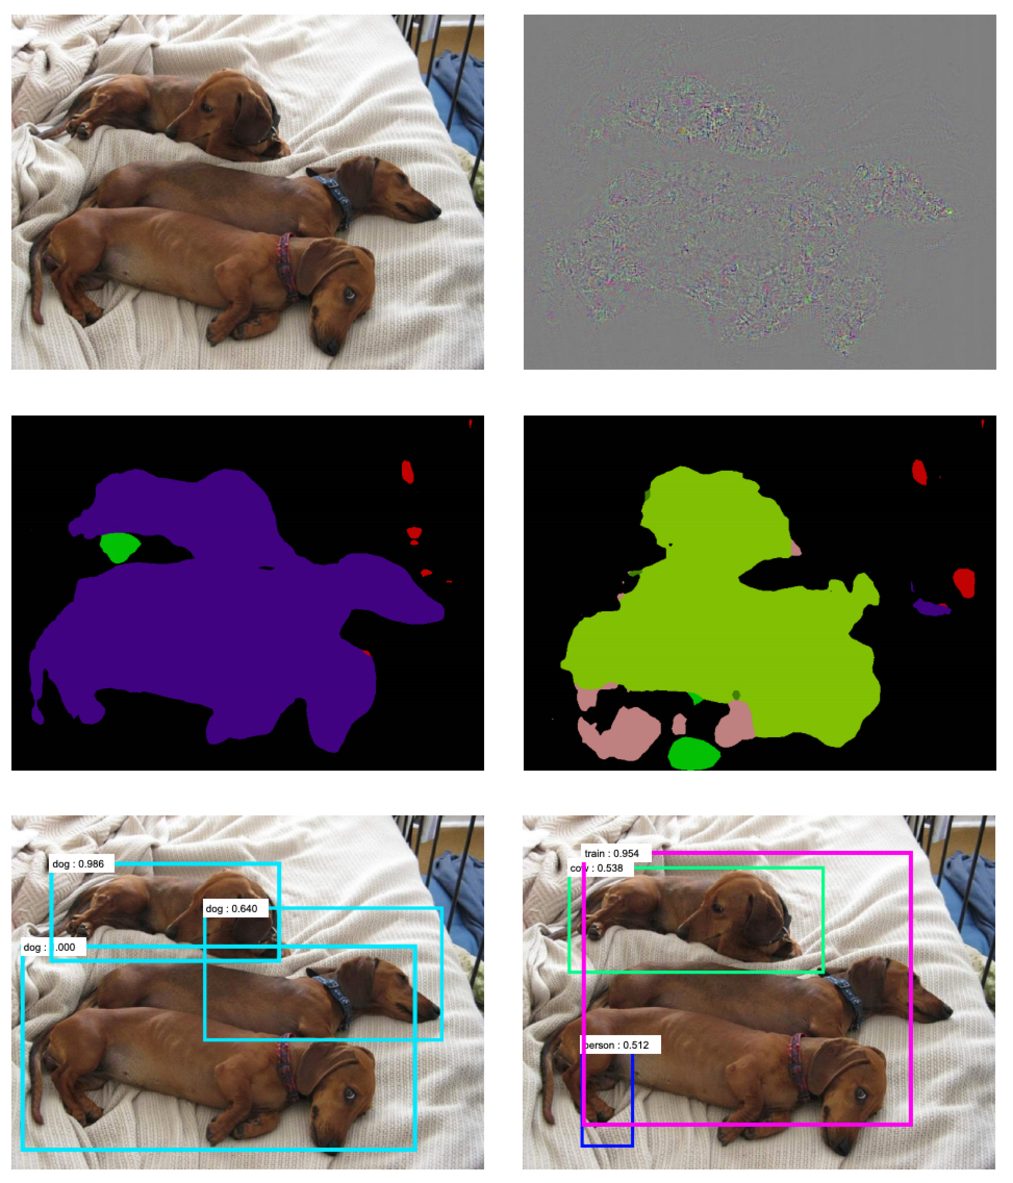
\includegraphics[width=10.0cm]{figures/adversarial-examples-example.pdf}
\end{center}
\caption{
object detection と segmentation に対する摂動とその効果の例.
上の行は左列が入力画像で右列が摂動, 真ん中の行は左列が入力画像に対する segmentation の結果で右列が adversarial examples に対する segmentation の結果, 下の行は object detection の結果である.
摂動に関しては画像として見やすいように大きさが 10 倍されている.
segmentation において, 紫色が {\it dog} のラベルで黄緑色が {\it train} ラベルである.
図は \cite{xie2017adversarial} より引用.
}
\label{fig:adversarial-examples-example}
\end{figure}
%

定量的な結果は object detection が図 \ref{fig:adversarial-examples-result-object-detection} で segmentation が図 \ref{fig:adversarial-examples-result-segmentation} である.
摂動の作成は, object detection では ZF と VGG, segmentation では AlexNet と VGG で実施しており, ResNet は予測モデルとしてのみ使用している.
どちらの結果も white box attack では大きく性能が低下しており, 提案手法の攻撃が確かに機能していることが分かる.
モデルの構造が似ている場合は transferability も高いが, 一方で ResNet への影響は少なく, 攻撃性能はかなりモデル構造に依存している.
摂動を足し合わせることでそれぞれのモデルの性能が低下しているため, 摂動にある種の線形性があることも伺える.
また, permutate した結果はほとんど摂動なしの結果と変わらないことから, 摂動は単にその大きさが重要なのではなく, 意味のある位置に配置して摂動が増幅されるようになっている必要があることも示されている.
%
\begin{figure}[htbp]
\begin{center}
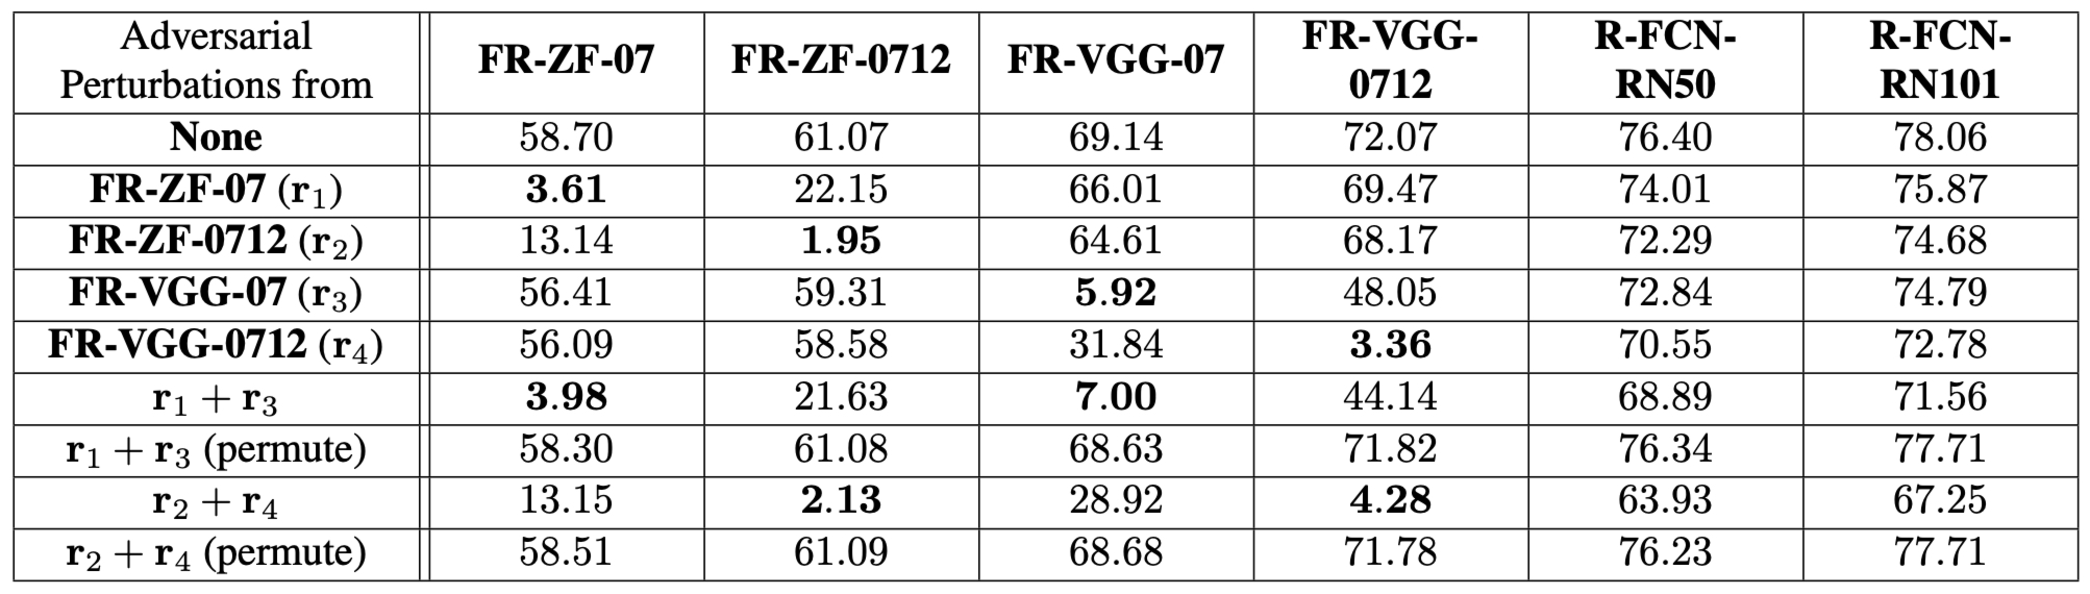
\includegraphics[width=14.0cm]{figures/adversarial-examples-result-object-detection.pdf}
\end{center}
\caption{
PascalVOC2007 の 4,952 枚のテストデータに対する結果.
表の値は mAP で $r$ は摂動 $\omega$ と対応している.
$r_1 + r_3$ (permute) は, それぞれのモデルで得られた摂動を足した後に, 行や列をランダムに入れ替えて作成した摂動である.
図は \cite{xie2017adversarial} より引用.
}
\label{fig:adversarial-examples-result-object-detection}
\end{figure}
%
%
\begin{figure}[htbp]
\begin{center}
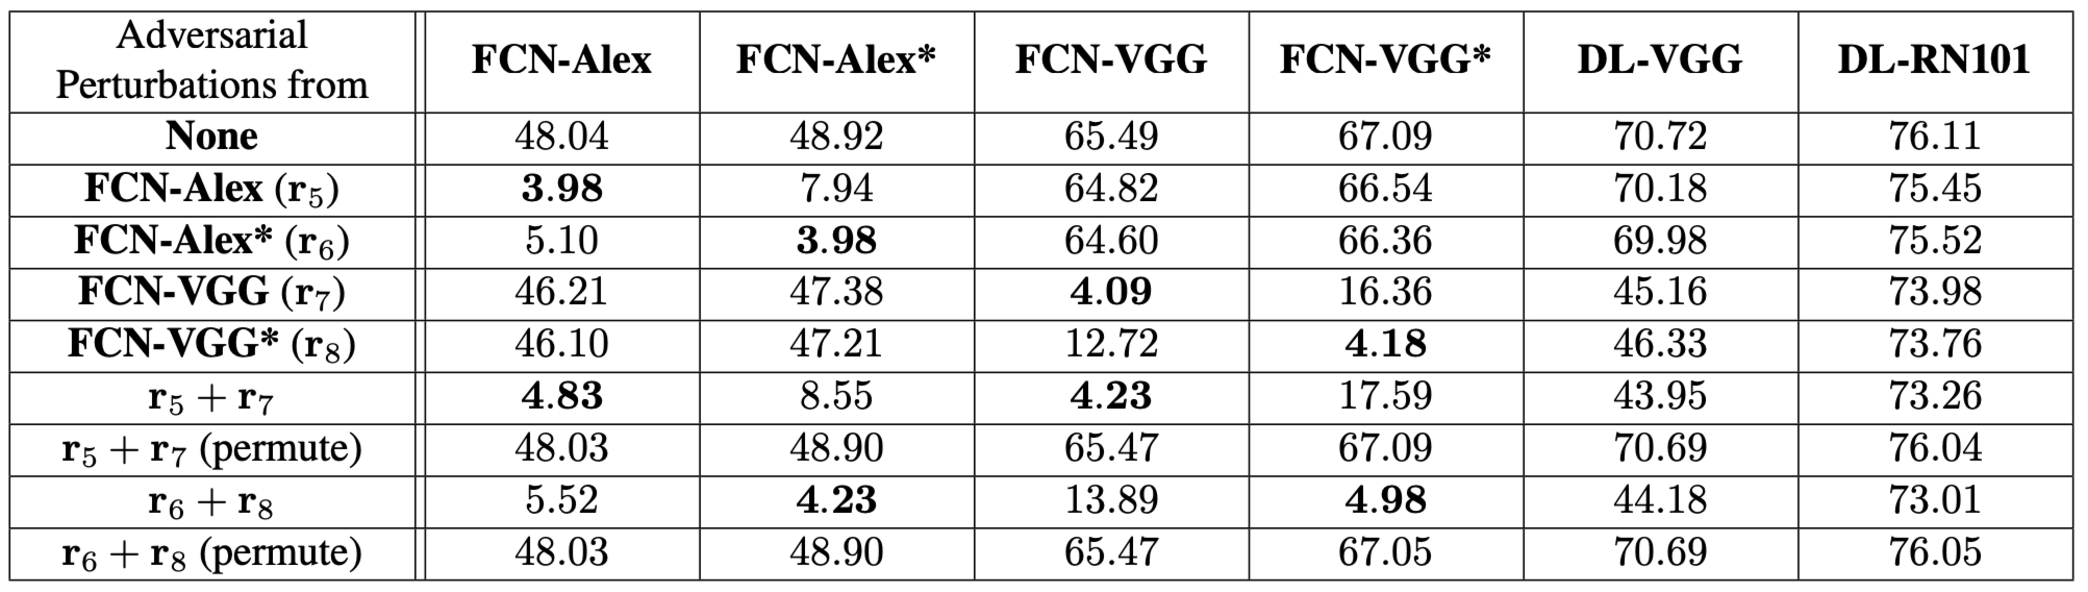
\includegraphics[width=14.0cm]{figures/adversarial-examples-result-segmentation.pdf}
\end{center}
\caption{
PascalVOC2007 の 736 枚の検証データに対する結果.
表の値は mIoU で $r$ は摂動 $\omega$ と対応している.
$r_1 + r_3$ (permute) は, それぞれのモデルで得られた摂動を足した後に, 行や列をランダムに入れ替えて作成した摂動である.
図は \cite{xie2017adversarial} より引用.
}
\label{fig:adversarial-examples-result-segmentation}
\end{figure}
%

認識のしづらさとして定義した式 \ref{eq:adversarial-examples-imperceptibility} を用いると, どの摂動に対しても $1.5 \sim 3.0 \times 10^{-3}$ という値になっていてそこまで大きな違いはない.
図 \ref{fig:adversarial-examples-example} で見たように, classification と同様に人間にとっては違いは認識しづらいレベルになっている.

この手法は, classification に対する adversarial examples を object detection は segmentation に拡張したという点で興味深い.
object detection に対する adversarial examples は自動運転などの応用を考えると高い重要性を持っており, このような論文をきっかけに攻撃やその防御方法などが広く研究されるようになってきている.
object detection に対する adversarial examples が出始めたころは \cite{lu2017no} で自動運転においては撮影の距離や角度が変わるので誤認識はされないという議論もなされたりもしたが, その後すぐに物理的環境の変化があっても高い割合で誤認識させる攻撃手法も提案され, 以降は object detection の研究も盛んに進められていて, この分野の発展の早さが感じられる.



\subsection{DARTS: Deceiving Autonomous Cars with Toxic Signs}
\label{subsec:darts}
%
\begin{table}[htbp]
\begin{center}
\begin{tabular}{|c|c|}
\hline
分類の観点 & この手法が該当するもの \\
\hline
Digital $\lor$ Physical & Physical \\
Classifier $\lor$ Detector & Detector-Classifier パイプライン \\
摂動作成時に使用するデータ & 攻撃対象データ \\
摂動の加え方 & 対象物のみ \\
知覚しづらさの定義 & $l_2$ \\
White box $\lor$ Black box & White box \\
\hline
\multicolumn{2}{|c|}{公式実装: \href{https://github.com/chawins/DART}{https://github.com/chawins/DART}} \\
\hline
\end{tabular}
\label{tb:darts-summary}
\end{center}
\end{table}
%

これは \cite{sitawarin2018darts} によって提案された手法であり, 動画から Canny 法によるエッジ検出と Hough 変換を使って標識部分を切り出し, それを classifier で分類するというパイプラインに対して異なる標識と誤認識させる.
また, 摂動を加える以外にも, 見る角度によって異なる標識になるようなレンチキュラー印刷による攻撃手法も提案している.

この手法は detector を攻撃対象とした physical な攻撃ではあるが, 想定している予測モデルは detector ではなく, 図 \ref{fig:darts-pipeline} のように, DNN 以前の手法での detector と DNN による classifier をつなぎ合わせたパイプラインを攻撃対象としている点が特徴的である.
%
\begin{figure}[htbp]
\begin{center}
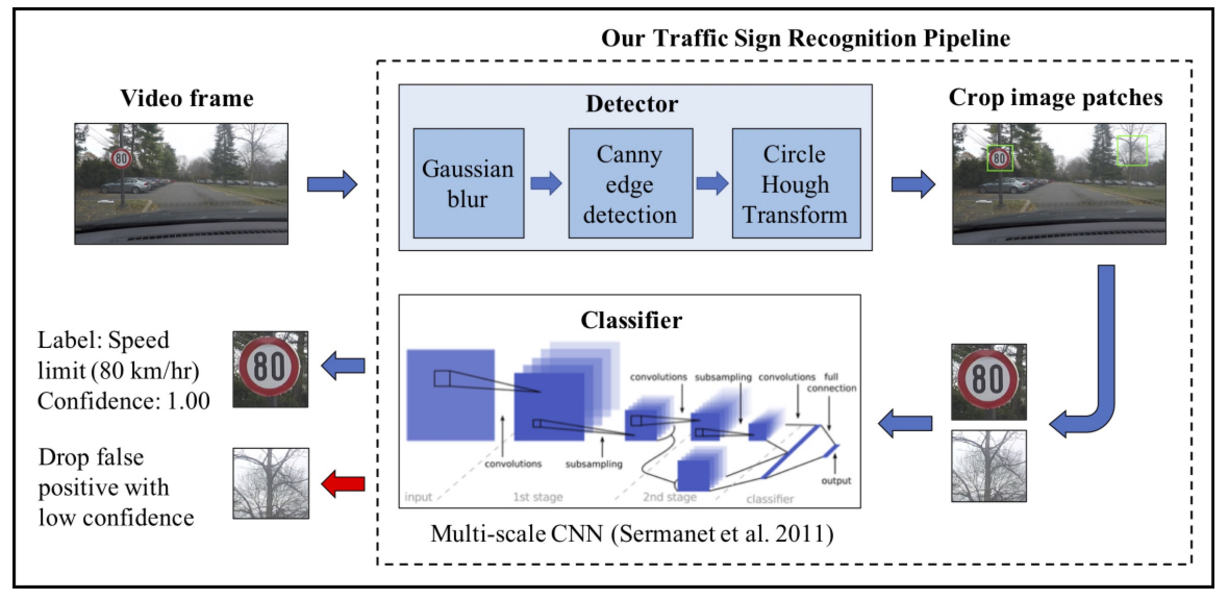
\includegraphics[width=14.0cm]{figures/darts-pipeline.pdf}
\end{center}
\caption{
攻撃対象となる detector-classifier pipeline の概略図.
動画の書くフレームにおいて, まず Canny 法でエッジを検出してからハフ変換を用いて標識の円部分を検出し, 該当部分を cropping して classifier で予測するという流れになっている.
図は \cite{sitawarin2018darts} より引用.
}
\label{fig:darts-pipeline}
\end{figure}
%

全体としては自動運転システムを対象にした攻撃になっているが, adversarial examples で攻撃するのは標識部分を crop した画像を入力とする classifier である.
そのため, adversarial examples の作り方自体は classifier を対象とした場合と違いはない.
この論文では標識のみをターゲットにしているため, 円形の対象物に特化した手法で, Canny 法でエッジを検出することで円部分のみを切り出す mask を作る.
mask を使うというのは \ref{subsec:robust-physical} 節で紹介した手法と同様のアプローチで, 標識部分のみに摂動を加えるためにこの mask を用いている.
摂動を作成するために解く最適化問題としては以下を設定している.
%
\begin{eqnarray}
\min_{\omega} \left[ \frac{c}{B} \sum_b^B F(\tau_b (x + M \cdot \omega)) + \max (\| \omega \|_p, L) \right].
\label{eq:darts-optimization}
\end{eqnarray}
%
ここで, $B$ はバッチサイズ, $F(x) = \max ( \max_{j \neq t} \{f_{\text{logit}, j} (x)\} - f_{\text{logit}, t} (x), - K)$ は loigt loss, $M$ は標識部分のみを残す mask, $\tau_b$ は回転などの幾何学変換, である.
$c, K, L$ はうまく解が求まるようにヒューリスティックに調整するパラメタである.
ノルムは任意のものを使えるが, 論文では $p = 1$ を採用している.
この最適化問題を Adam \cite{kingma2014adam} を用いて解くことで摂動を作成する.
adversarial examples 作成の全体図は図 \ref{fig:darts-attack-pipeline} である.
%
\begin{figure}[htbp]
\begin{center}
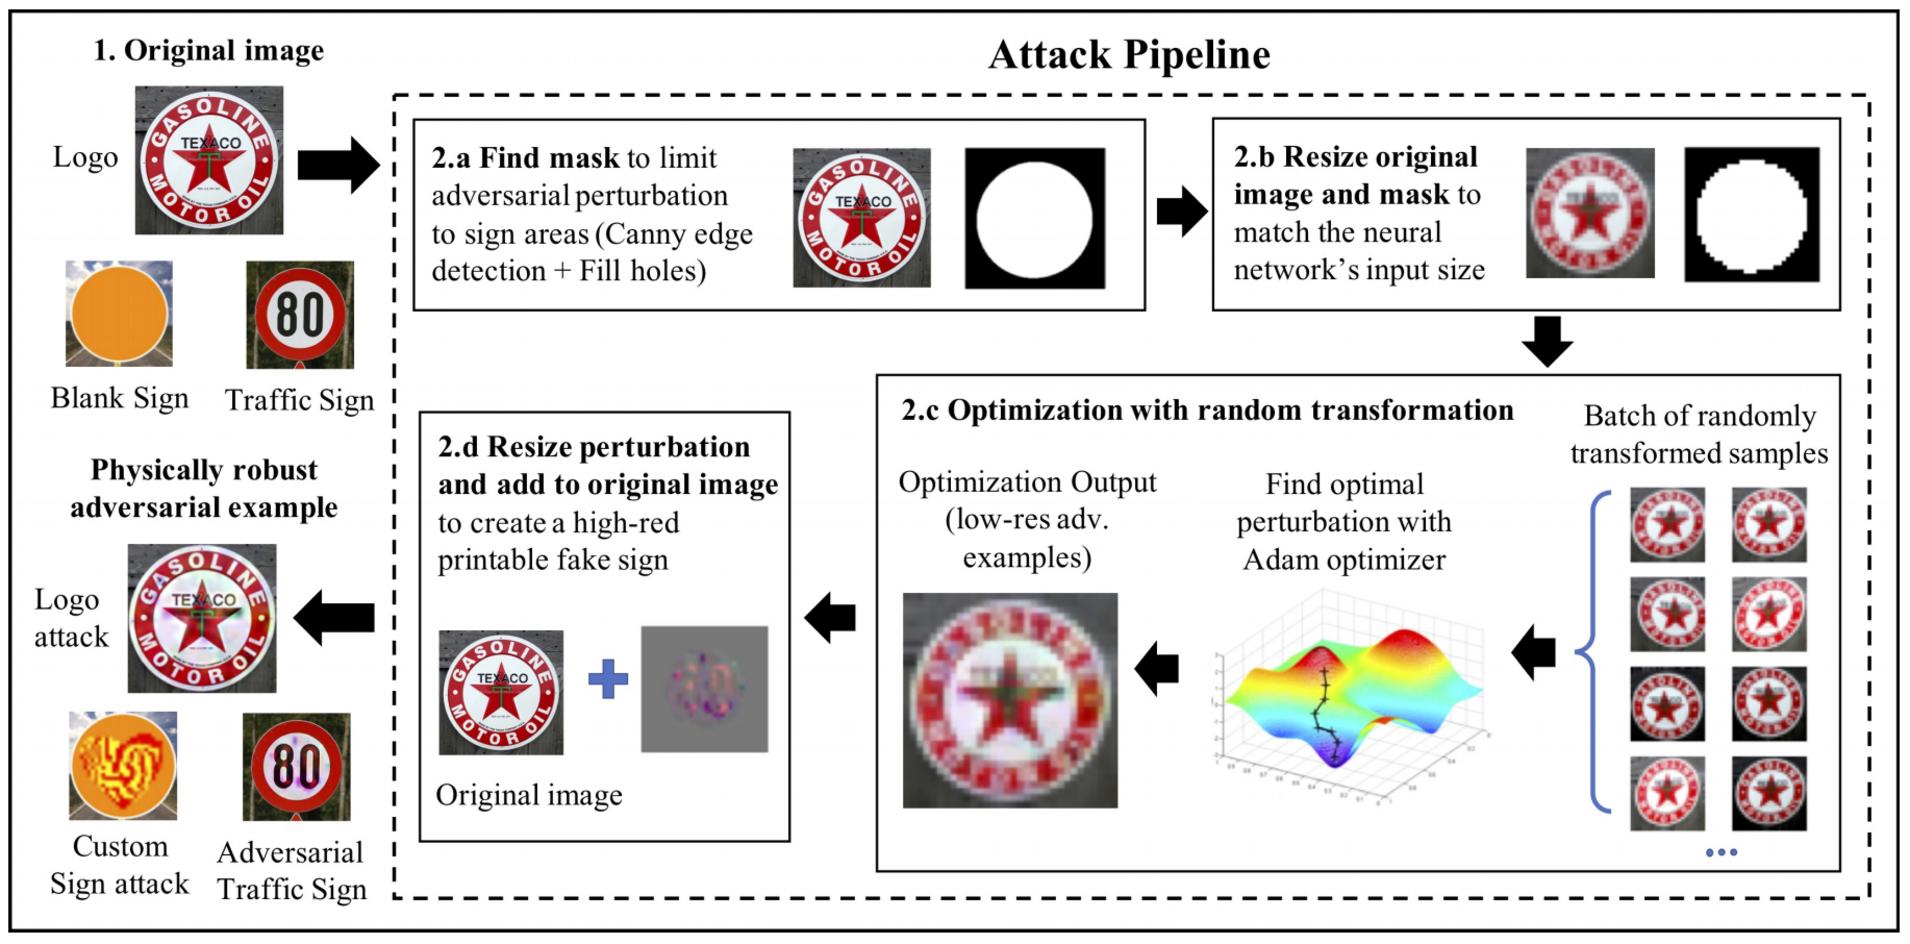
\includegraphics[width=14.0cm]{figures/darts-attack-pipeline.pdf}
\end{center}
\caption{
adversarial examples 作成の手順.
標識部分を切り出す mask を作成し, 様々な幾何学変換を加えたサンプルを誤認識させる摂動を式 \ref{eq:darts-optimization} を Adam で解くことで作成する.
図は \cite{sitawarin2018darts} より引用.
}
\label{fig:darts-attack-pipeline}
\end{figure}
%

摂動が作成できれば, それは円形で標識の形にマッチしているので, 紙などに印刷して標識の上から貼り付けることで自動運転システムを攻撃することができる.
この論文では, 標識以外にも円形のロゴに対する摂動や, 無地の円形図形に特定の模様や文字の摂動 (そのような mask を準備すれば実現できる) を作成している.
その結果が図 \ref{fig:darts-example} であり, 作成した摂動が classifier を誤認識させていることが分かる.
%
\begin{figure}[htbp]
\begin{center}
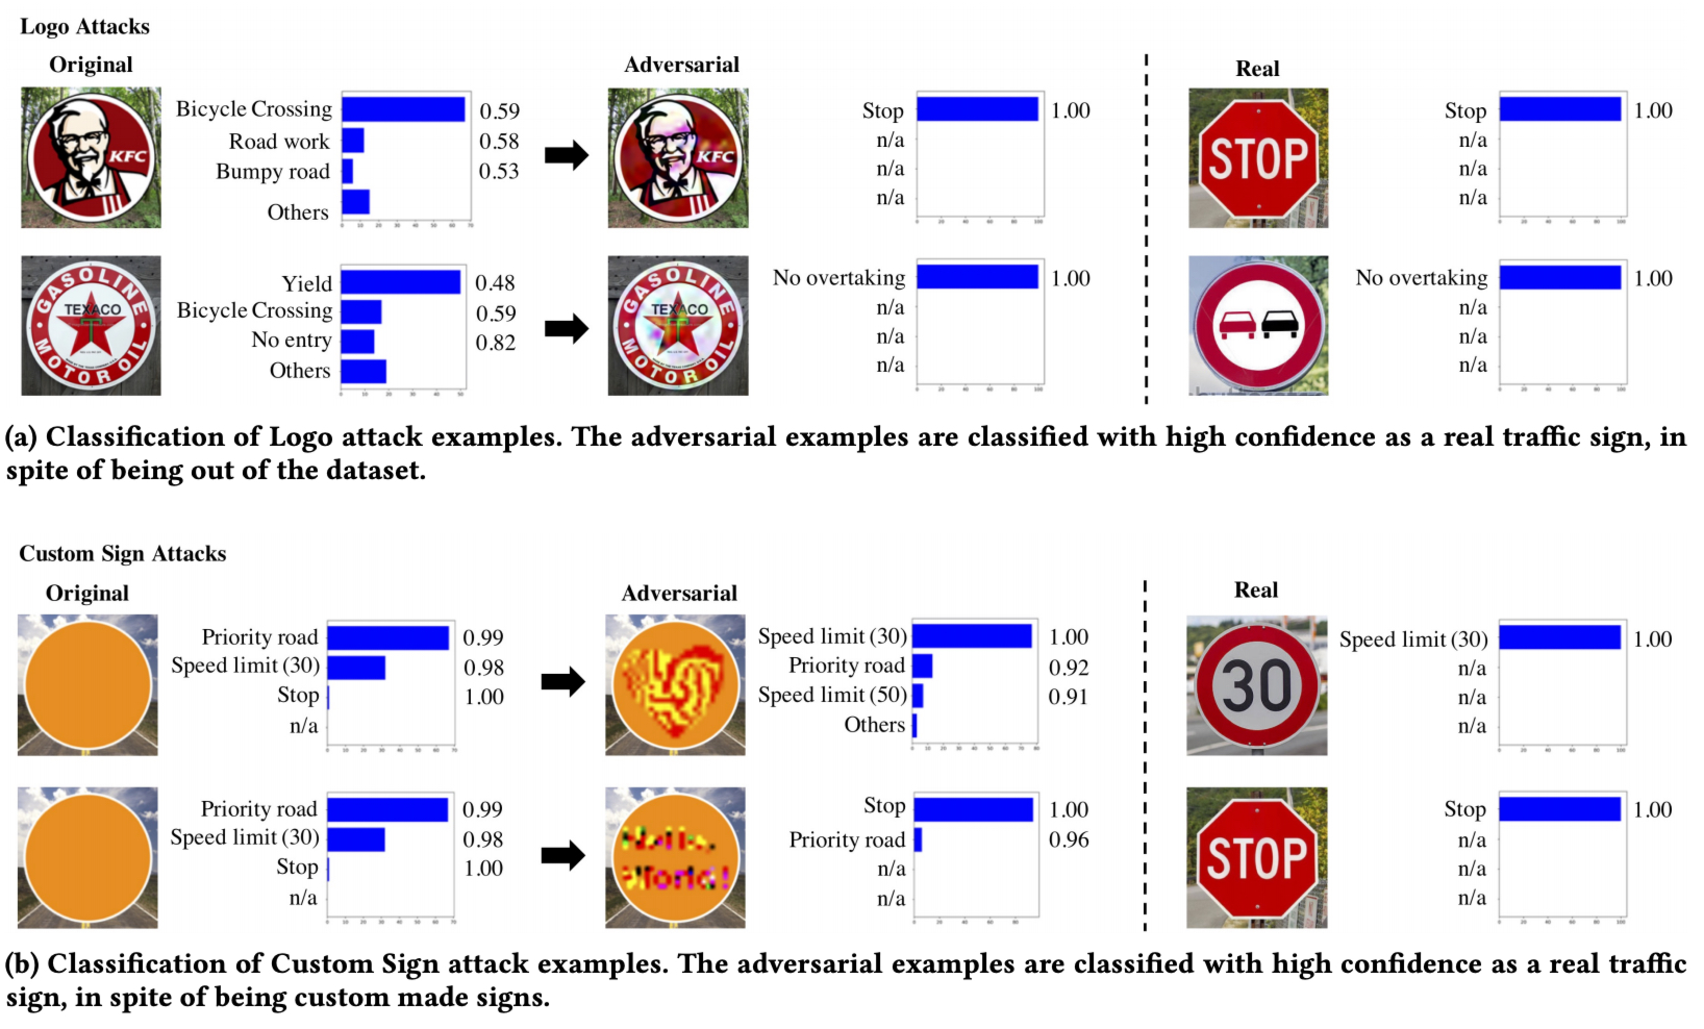
\includegraphics[width=14.0cm]{figures/darts-example.pdf}
\end{center}
\caption{
作成した摂動の例とそれに対する classifier の予測結果.
予測結果のラベルと数値は 100 個の異なる幾何学変換を加えて予測した際の top-1 の結果をカウントしたものと confidence の平均を表す.
Original は摂動を加える前の画像で, classifier は標識のラベルを予測するようになっているのでうまく予測できていないが, 摂動を加えたものは明白に何かの標識に誤認識している.
Real は実際の標識画像に対して classifier が適切に予測していることを示している.
図は \cite{sitawarin2018darts} より引用.
}
\label{fig:darts-example}
\end{figure}
%

実験は様々なものを実施しているが, 特に興味深い drive-by test のみに言及する.
作成した摂動は前述のように印刷して physical attack として利用できるため, 実験用に adversarial examples となる標識を準備し, 車に GoPro HERO5 を設置して撮影した動画で検証をしている.
モデルは multi-scale CNN \cite{sermanet2011traffic} を用いている.
結果は図 \ref{fig:darts-result-table} の通りで, 提案手法の攻撃が physical attack として有効に機能していることが示されている.
black box attack の攻撃成功率がやたらと高く出ているが, ここでの black box attack は攻撃者はモデルとしては同じものを用いるが学習自体は別個に実施して, 摂動作成時には実際の予測モデルではなく自分が学習したモデルを使う, という設定になっているためである.
これは実質 white box と言ってよいだろう.
%
\begin{figure}[htbp]
\begin{center}
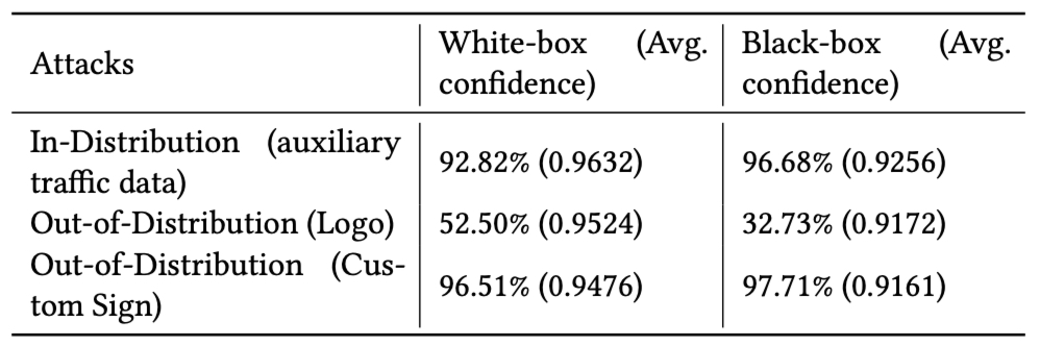
\includegraphics[width=12.0cm]{figures/darts-result-table.pdf}
\end{center}
\caption{
adversarial examples となる標識を設置して, 実際に車から撮影した動画で誤認識率 (1 - 正答率) を測定した結果.
auxiliary traffic data は標識の画像データを基にして摂動を作成した場合となる.
図は \cite{sitawarin2018darts} より引用.
}
\label{fig:darts-result-table}
\end{figure}
%

また, この論文ではレンチキュラー印刷による攻撃手法も提案している.
レンチキュラー印刷とは凸型の表面を利用した印刷方法で, 見る角度によって異なる対象物が見えるものである.
車載カメラが運転者の目線よりも低い位置に付けられるということを想定し, 下から撮影すると別の標識に認識されるような印刷物を作成し, 期待通りに攻撃が成功したことも報告している.
これはこれで興味深いが, DNN に対する adversarial examples とは独立な手法であるため, 本書ではこれ以上は立ち入らない.

この手法は単一の DNN detector ではなく, DNN 以前の手法による detector と DNN classifier パイプラインに対する攻撃手法を提案したという点が興味深い.
近年の DNN の性能を考えればこのようなパイプラインを実際に使用する可能性はあまり高くはないと思われるが, physical attack でありながらも標識の classifier をターゲットにすることで誤認識率の高い adversarial examples を作成することに成功している.
自動運転に限らず, いくつかのモデルを組み合わせたパイプラインに対して, 攻撃対象を絞ることで攻撃効率を高めるというのは攻撃側にとっては有効な選択肢になるだろう.



\subsection{ShapeShifter: Robust Physical Adversarial Attack on Faster R-CNN Object Detector}
\label{subsec:shapeshifter}
%
\begin{table}[htbp]
\begin{center}
\begin{tabular}{|c|c|}
\hline
分類の観点 & この手法が該当するもの \\
\hline
Digital $\lor$ Physical & Physical \\
Classifier $\lor$ Detector & Detector \\
摂動作成時に使用するデータ & 攻撃対象データ \\
摂動の加え方 & 対象物のみ \\
知覚しづらさの定義 & $l_2$ \\
White box $\lor$ Black box & White box \\
\hline
\multicolumn{2}{|c|}{公式実装: \href{https://github.com/shangtse/robust-physical-attack}{https://github.com/shangtse/robust-physical-attack}} \\
\hline
\end{tabular}
\label{tb:shapeshifter-summary}
\end{center}
\end{table}
%

これは \cite{chen2018shapeshifter} によって提案された手法であり, Faster-RCNN に対して候補領域の予測に対する loss が高まるように摂動を作り攻撃をする\footnote{
技術的な内容とはあまり関係がないが, shapeshifter とは様々な姿に変身することができる妖怪のことである.
}.

この手法は detector をターゲットにして, physical attack でも誤認識率が高くなるような摂動を作成したという点が特徴的である.
それを実現するために, mask と classifier と比べて強めの摂動を用いている.

まず, classifier に対する攻撃を構成する.
この手法ではピクセル値として $[-1, 1]$ の範囲を取るように画像を正規化する.
作成する adversarial examples がこの範囲に収まるようにするためには $\tanh$ を利用する.
CW の方法に従い, 以下の最適化問題を解くことで摂動を作成する.
%
\begin{eqnarray}
\argmin_{x_{\text{adv}}} \left[ J (f, \tanh (x_{\text{adv}}), y_{\text{atk-tgt}}) + c \cdot \| \tanh (x_{\text{adv}}) - x \|_2 \right].
\label{eq:shapeshifter-classifier}
\end{eqnarray}
%
次にこれを physical attack に適したものにするために特定の対象物に限定することを考える.
これは \ref{subsec:darts} 節で紹介した手法と同様で重要な点は二つあり, 一つは mask を用いて対象物にのみ摂動を加えるようにすることで, もう一つは様々な幾何学変換を適用して異なる距離や角度から撮影しても摂動が有効になるようにすることである.
ここでは, ある特定の対象物部分のみの画像を $x_o$ として mask の処理を $M_{x^o} (x)$ とし,  幾何学変換を $t(x)$ とする.
これらを用いて式 \ref{eq:shapeshifter-classifier} を変更すると以下のように書ける.
%
\begin{eqnarray}
\argmin_{x_{\text{adv}}} \mathbb{E}_{x \sim p_x, t \sim p_t} \left[ J (f, t(M_{x^o} (\tanh (x_{\text{adv}}))), y_{\text{atk-tgt}}) + c \cdot \| \tanh (M_{x^o} (x_{\text{adv}})) - x \|_2 \right].
\label{eq:shapeshifter-classifier-object-oriented}
\end{eqnarray}
%
ただし, $x$ はある特定のクラスに属するもので何かしらの分布から生成されているものとし, $t$ も何かしらの変換の分布から生成されていると定式化している.

これを detector に拡張することを考える.
Faster-RCNN は RPN で検出した候補領域で予測をするモデルであるので, それを考慮して mask した上での候補領域 $r_1, \dots, r_m$ を対象にした loss に変更すればよい.
%
\begin{eqnarray}
\argmin_{x_{\text{adv}}} \mathbb{E}_{x \sim p_x, t \sim p_t} \left[ \frac{1}{m} \sum_{r_i \in RPN (t(M_{x^o} (\tanh (x_{\text{adv}}))))} J (f, r_i, y_{\text{atk-tgt}}) + c \cdot \| \tanh (M_{x^o} (x_{\text{adv}})) - x \|_2 \right].
\label{eq:shapeshifter-detector}
\end{eqnarray}
%
これは候補領域毎に loss を計算しているという違いはあるが, 本質的には classifier のものと同じである.
全ての候補領域が固定されていればこのままでよいが, NMS などの微分不可能な仕組みで候補領域が変更されるため, このままではこの最適化を解くのは難しい.
この論文では, まずは RPN だけを対象にして最適化を Adam などを使って近似的に解き, RPN が返す候補領域を固定してしまう.
予測ステージではこの予測領域は固定したまま予測モデル部分に対して改めて最適化を解くことで, adversarial examples を作成する.
論文ではこの近似で十分に良い adversarial examples が作成できると主張している.

adversarial examples 作成のためのデータは MSCOCO2017 データ \cite{lin2014microsoft} の {\it stop sign} クラスを用いる.
これは mask を作成するのが楽で, かつ印刷をして physical attack の実験をするのにも適している.

実際に physical attack をしてみた例が図 \ref{fig:shapeshifter-result-physical} である.
クラスが {\it sports ball} の場合は狙い通りに誤認識させることが難しいが, {\it person} もしくは utntargeted の場合は攻撃が成功しているのが見て取れる.
%
\begin{figure}[htbp]
\begin{center}
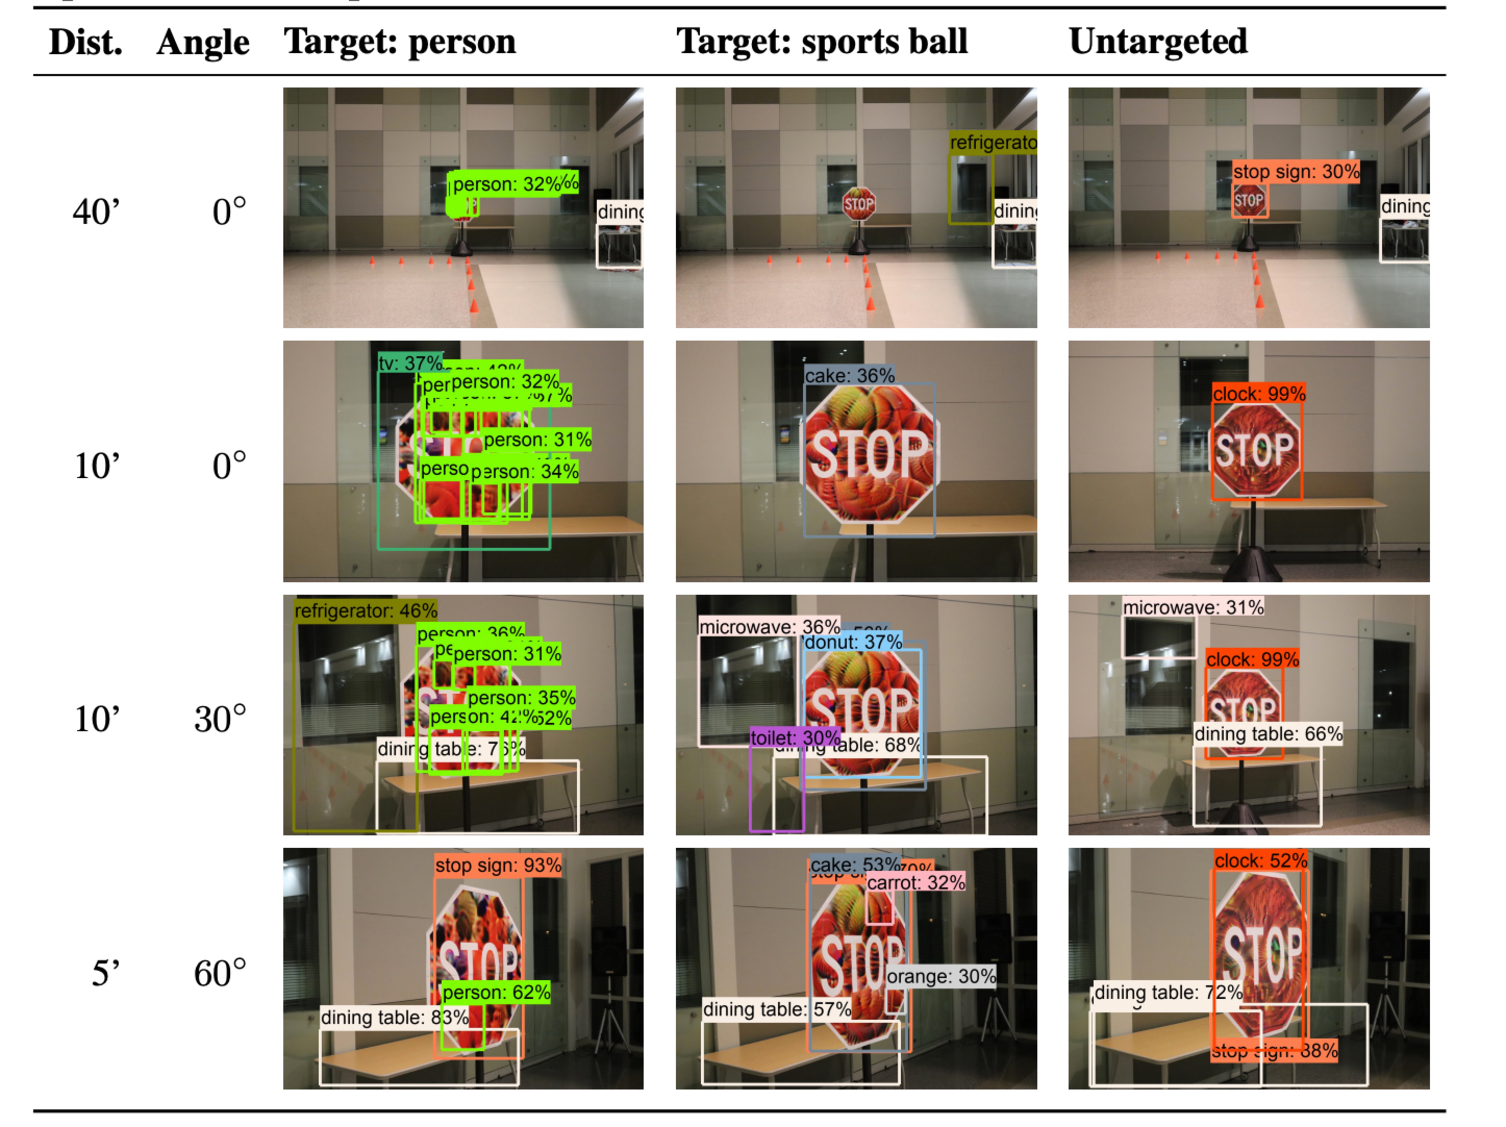
\includegraphics[width=14.0cm]{figures/shapeshifter-result-physical.pdf}
\end{center}
\caption{
physical attack の例.
MSCOCO2017 の {\it stop sign} クラスの画像で摂動を作成し, それをプリントしたものを様々な距離や角度から撮影して Faster-RCNN で予測している.
図は \cite{chen2018shapeshifter} より引用.
}
\label{fig:shapeshifter-result-physical}
\end{figure}
%

physical attack は性能の測定が難しく, 従来手法では雑に動画を撮って各フレームで調べるという程度でしか調べられていなかったが, この論文では静止画限定ではあるがもう少し定量的な評価指標を構築している.
図 \ref{fig:shapeshifter-measurement} のように距離と角度を指定して撮影し, それぞれの画像で正答率を調べることで physical attack の異なる環境での有効性を検証している.
%
\begin{figure}[htbp]
\begin{center}
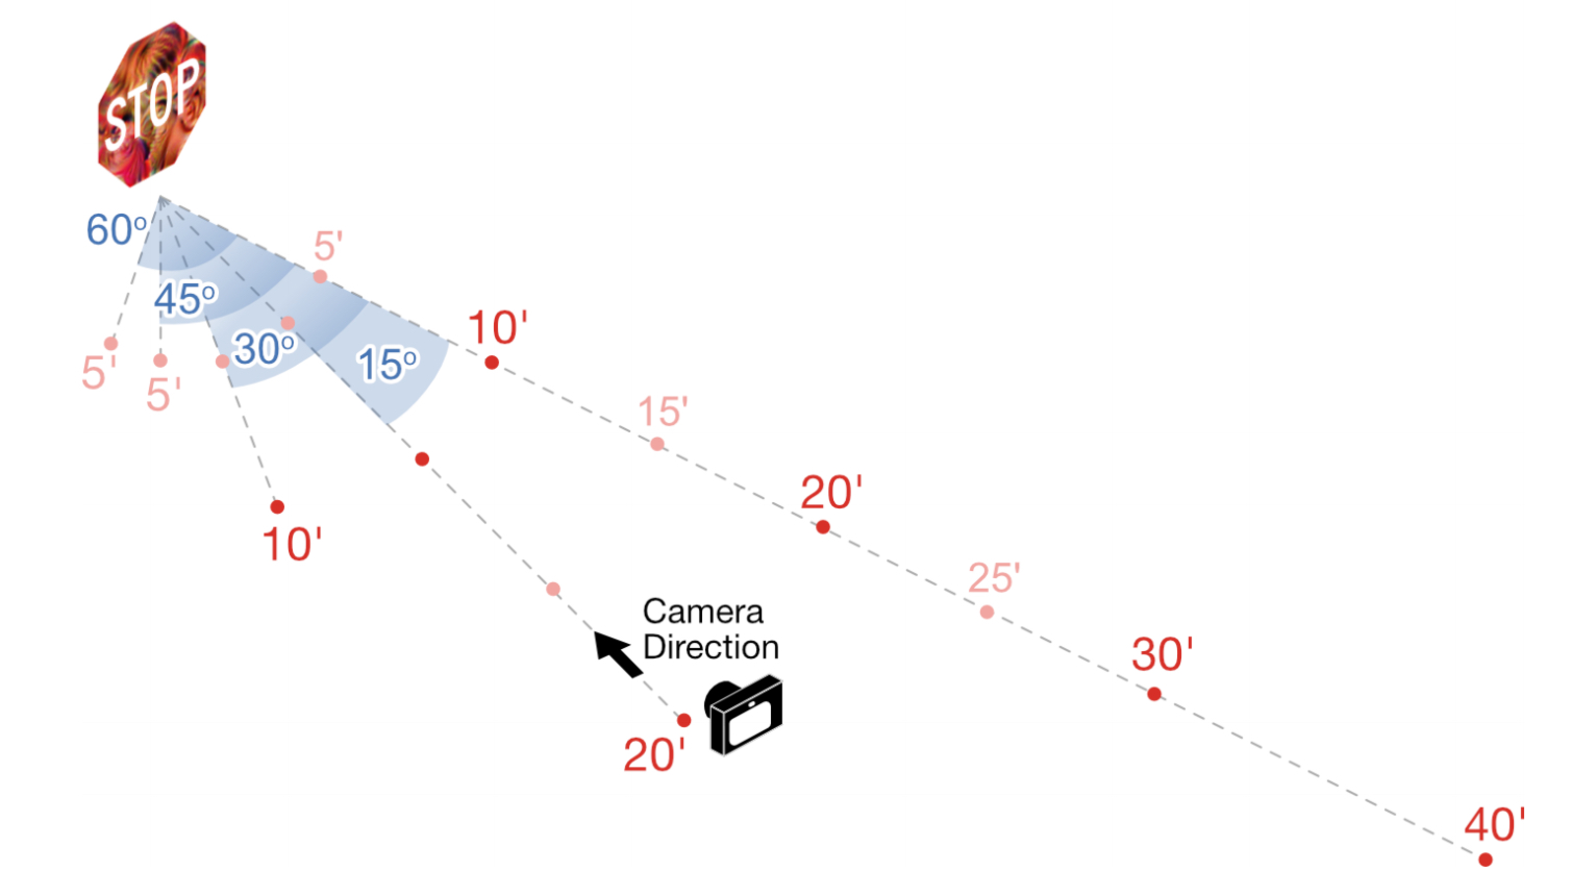
\includegraphics[width=12.0cm]{figures/shapeshifter-measurement.pdf}
\end{center}
\caption{
静止画の physical attack に対する測定方法.
角度は $\{0^{\circ}, 15^{\circ}, 30^{\circ}, 45^{\circ}, 60^{\circ}\}$ で, 距離は角度に応じて $5$ フィート (約 $1.5$ メートル) から $40$ フィート (約 $12$ メートル) である.
図は \cite{chen2018shapeshifter} より引用.
}
\label{fig:shapeshifter-measurement}
\end{figure}
%

静止画で定量的に測定した結果が図 \ref{fig:shapeshifter-result-table} である.
どのクラスに間違えさせるかで性能も変わってくるが, {\it person} ではほとんどの距離や角度で誤認識させることに成功している.
ただし, 角度がキツくなると誤認識させることは失敗している.
%
\begin{figure}[htbp]
\begin{center}
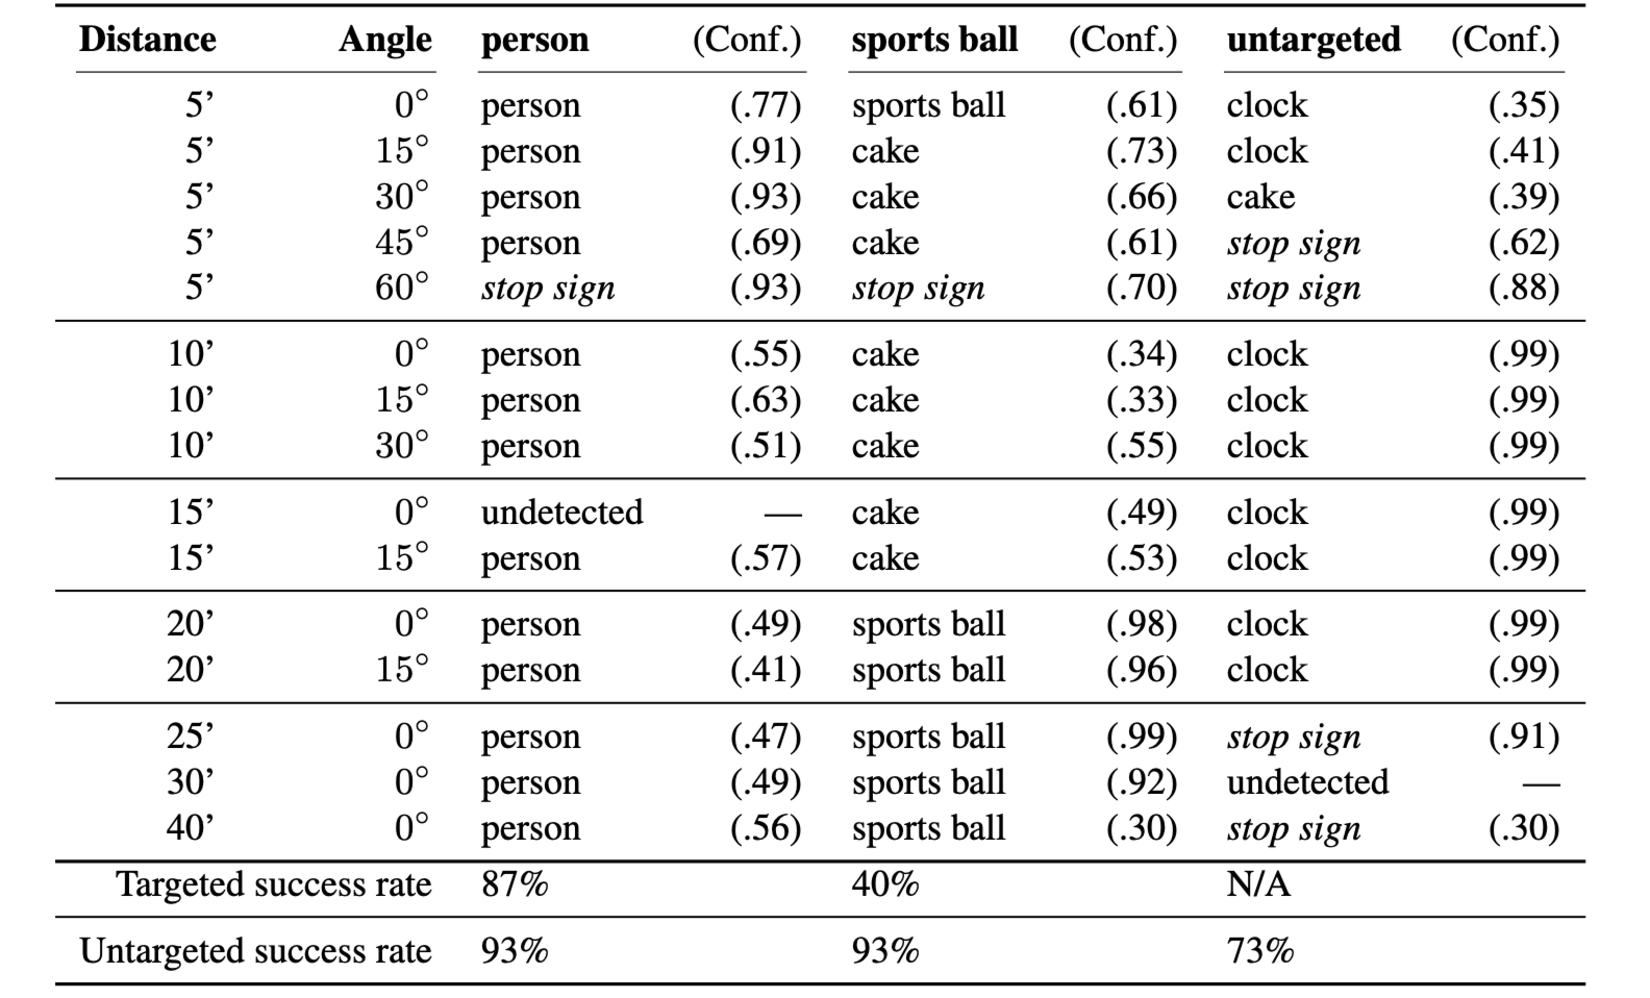
\includegraphics[width=14.0cm]{figures/shapeshifter-result-table.pdf}
\end{center}
\caption{
physical attack に対する静止画の定量的評価.
図 \ref{fig:shapeshifter-result-physical} で定義した距離と角度で画像を撮影し, Faster-RCNN の予測結果の confidence が最も高いものを記載している.
success rate は攻撃成功率 (1 - 正答率) を表す.
図は \cite{chen2018shapeshifter} より引用.
}
\label{fig:shapeshifter-result-table}
\end{figure}
%

動画での検証も実施しており, 車からスマートフォンで動画を撮影して各フレームで Faster R-CNN の予測を評価している.
{\it person} クラスに誤認識させる摂動の場合, 405 フレーム中, 1 フレームは {\it stop sign}, 190 フレームは {\it person}, 残りの 214 フレームは検出されず, という結果になっている.
{\it sports ball} クラスに誤認識させる摂動も同じような結果だが, untargeted の場合はほとんどが未検出という結果になっている.
untargeted の場合になぜ静止画での評価との乖離が大きいかというのは著者はよく分からない.

この手法は, Faster-RCNN を対象にした physical attack として高い攻撃成功率を達成した点が興味深い.
physical attack で高い攻撃成功率を達成するためには摂動はかなり強いものにする必要があるが, mask と合わせて性能の高い physical attack を実現した.
また, 静止画ではあるが physical attack の定量的評価を提示したというのも重要な点である.
全部で 15 枚の予測であるので数としては心許ないが, 再現性や比較のために共通の評価方法が確立されることが期待される.



\subsection{Daedalus: Breaking Non-Maximum Suppression in Object Detection via Adversarial Examples}
\label{subsec:daedalus}
%
\begin{table}[htbp]
\begin{center}
\begin{tabular}{|c|c|}
\hline
分類の観点 & この手法が該当するもの \\
\hline
Digital $\lor$ Physical & Digital \\
Classifier $\lor$ Detector & Detector \\
摂動作成時に使用するデータ & 攻撃対象データ \\
摂動の加え方 & 画像全体 \\
知覚しづらさの定義 & $l_0, l_2$ \\
White box $\lor$ Black box & White box \\
\hline
\multicolumn{2}{|c|}{公式実装: \href{https://github.com/NeuralSec/Daedalus-attack}{https://github.com/NeuralSec/Daedalus-attack}} \\
\hline
\end{tabular}
\label{tb:daedalus-summary}
\end{center}
\end{table}
%

これは \cite{wang2019daedalus} によって提案された手法であり, NMS に対して摂動で攻撃を加えることで大量の誤った bbox を認識させるという攻撃手法である\footnote{
技術的な内容とは関係ないが, daedauls は日本語ではダイダロスで, ギリシャ神話においてミノタウルスを封じ込めるために迷宮を作った.
}.

この手法は detector の予測を間違えさせるというアプローチではなく, 大量の bbox が発生するように誤認識させるという点が特徴的である.

定式化のためにいくつか記法を導入する.
detector を $F(x) = \{ B^x, B^y, B^w, B^h, B^o, P \}$ という関数とする.
ここで, $n$ 個の bbox が存在するとき, $B^x = \{b^x_0, b^x_1, \dots, b^x_n\}$ と $B^y = \{b^y_0, b^y_1, \dots, b^y_n\}$ を bbox の左上の $(x,y)$ 座標, $B^w = \{b^w_0, b^w_1, \dots, b^w_n\}$ と $B^h = \{b^h_0, b^h_1, \dots, b^h_n\}$ を bbox の width と height とする.
さらに, $B^o = \{b^o_0, b^o_1, \dots, b^o_n\}$ を objectness のスコア, $P = \{p_0, p_1, \dots, p_n\}$ を $C$ 次元のクラス確率とする.
bbox があるクラス $\lambda \in \Lambda$ ($\Lambda$ は一般に複数クラスを含む) に属するものに対する攻撃を実現するために, 以下の 3 つの loss function を提案している.
%
\begin{eqnarray}
J_1 &=& \frac{1}{|\Lambda|} \sum_{\lambda \in \Lambda} \mathbb{E}_{i:\argmax(p_i) = \lambda} \left[ (b^o_i \cdot \max (p_i)  - 1)^2 + \mathbb{E}_{j:\argmax(p_j) = \lambda} \left[ IoU_{ij} \right] \right]. \\
J_2 &=& \frac{1}{|\Lambda|} \sum_{\lambda \in \Lambda} \mathbb{E}_{i:\argmax(p_i) = \lambda} \mathbb{E}_{i:\argmax(p_i) = \lambda} \left[ (b^o_i \cdot \max (p_i)  - 1)^2 + \left( \frac{b^w_i \cdot b^h_i}{W \times H} \right)^2 \right. \nonumber \\
&& \left. + \mathbb{E}_{j:\argmax(p_j) = \lambda} \left[ \frac{1}{(b^x_i - b^x_j)^2 + (b^y_i - b^y_j)^2} \right] \right]. \\
J_3 &=& \frac{1}{|\Lambda|} \sum_{\lambda \in \Lambda} \mathbb{E}_{i:\argmax(p_i) = \lambda} \left[ (b^o_i \cdot \max (p_i)  - 1)^2 + \left( \frac{b^w_i \cdot b^h_i}{W \times H} \right)^2 \right].
\label{eq:daedalus-loss}
\end{eqnarray}
%
ここで, $IoU_{i,j}$ は $i$ 番目と $j$ 番目の bbox の IoU であり, $W, H$ はそれぞれ画像の width と height である.
$J_1$ は第一項は $\lambda$ クラスに予測される bbox に関して $b^o_i \cdot \max (p_i)$ が 1 に近づくように要請するため, 多くの bbox が何かしらのクラスで検出されるように働く.
第二項は $\Lambda$ に含まれるクラスの bbox 同士の IoU が小さくなるように要請するため, それぞれが NMS で統合されずに別個のものと認識されやすくなるよう働く.
したがって, これら二項はどちらも数多くの bbox が検出されるような効果を発揮する.
$J_2, J_3$ の第二項は小さな bbox を作るよう要請するもので, $J_2$ の第三項はそれぞれの bbox の位置が離れるよう要請するものである.

上記の loss function を用いた攻撃手法がアルゴリズム \ref{alg:daedalus-alg} である.
loss function $J$ は上記の 3 つの loss のうちどれかを使い, 全体の loss は $\| \omega \|_p + c \cdot J(x)$ という形でこれを最小化する $x_{\text{adv}}$ を見つけるのと, 二分探索で最適な重み $c$ も見つけている.
ノルムは $p = 0, 2$ の場合を使うことになり, $l_2$ ノルムのように微分可能な場合はこのままのアルゴリズムでよいが, $l_0$ ノルムのように微分不可能な場合は各 iteration で勾配が最大になる要素だけを残して他の要素は 0 にするという処理を施す.
%
\begin{algorithm}
\caption{Daedalus attack のアルゴリズム}
\label{alg:daedalus-alg}
\begin{algorithmic}[1]
    \State Input: $x, \Lambda, \gamma$, bin\_steps, $\eta$, max\_iter, $c_{\text{max}}, c_{\text{min}}$
    \State Output: adversarial examples $x_{\text{adv}}$
	\State 初期化: $c \leftarrow 10, loss_{\text{init}} \leftarrow J(x), \delta \leftarrow 0, x^* \leftarrow x + \omega$.
	\For {0 から bin\_steps までの各 $n$}
	\For {0 から max\_iter までの各 $i$}
	\State $\Lambda$ から bbox を選択.
	\State 摂動を更新: $\omega \leftarrow \omega - \eta \nabla_{\omega} \left[ \| \omega \|_p + c \cdot J(x^*). \right]$
	\State 摂動を加えて $x^*$ を更新: $x^* \leftarrow x^* + \omega$.
	\EndFor
	\State 見つかった $x^*$ の中でベストなものを選択: $x_{\text{adv}} \leftarrow \ \text{best of } x^*$.
	\If {$J(x^*) \leq loss_{\text{init}} \cdot (1 - \gamma)$}
	\State $c_{\text{max}}$ を更新: $c_{\text{max}} \leftarrow \min (c, c_{\text{max}})$.
	\State $c$ を更新: $c \leftarrow 0.5 \cdot (c_{\text{max}} + c_{\text{min}})$.
	\Else
	\State $c_{\text{min}}$ を更新: $c_{\text{min}} \leftarrow \max (c, c_{\text{min}})$.
	\State $c$ を更新: $c \leftarrow 0.5 \cdot (c_{\text{max}} + c_{\text{min}})$.
	\EndIf
	\EndFor
\end{algorithmic} 
\end{algorithm}

実験では pre-trained の YOLO-v3 \cite{redmon2018yolov3} モデルと MSCOCO2017 validation データを用いる.
$\Lambda$ として全 80 クラスを用いて, adversarial examples 作成に時間が掛かるため評価はランダムにサンプリングした 100 件のデータで実施する.
評価指標としては通常の mAP とに加えて, bbox を大量に誤検出させるという攻撃手法であるため, False Positive (FP) rate を以下のように定めて定量的に評価する.
%
\begin{eqnarray}
\text{(FP rate)} = \frac{N_\phi + 1}{N + 1}.
\label{eq:daedalus-fp}
\end{eqnarray}
%
ここで, $N_\phi$ は検出した false positive の bbox の数 (これは ground truth が分かっているので計算できる) で, $N$ はモデルが検出した bbox の数.
これらは NMS の閾値で変化しうるものだが, 予備実験において閾値の影響は 1\% 未満であることが示されている.

本実験に入る前の予備実験として, 提案した loss function の中でどれが良いかを調べる.
MSCOCO2017 のデータからランダムに 10 件を選び, $l_2$ ノルムの場合でアルゴリズム \ref{alg:daedalus-alg} を実施し, 完成した画像で adversarial examples が目視で確認できた割合 (success rate) を測定した結果が図 \ref{fig:daedalus-loss-exp} である.
loss は $(1 - \gamma)$ という factor を掛けてそれを下回る場合は $c_{\text{max}}$ を小さくして最終的な $c$ も小さくなるため, $\gamma$ が小さい場合は adversarial examples が作成できない場合が多くなる.
success rate と一枚あたりの処理時間がどちらも優れているのは $J_3$ であるため, 以降では $J_3$ を用いる.
%
\begin{figure}[htbp]
\begin{center}
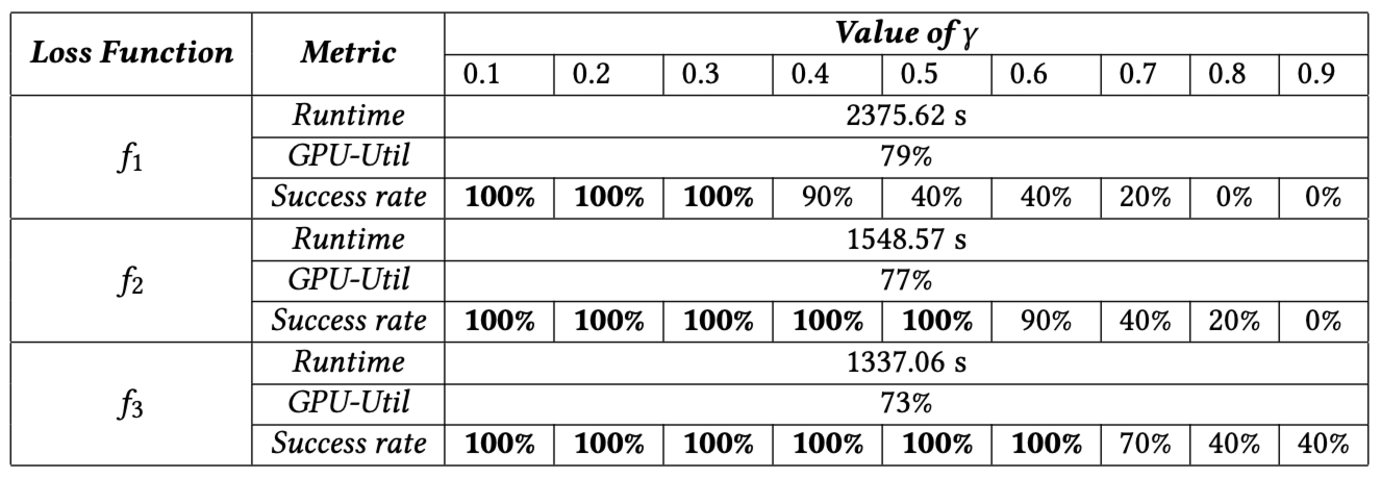
\includegraphics[width=14.0cm]{figures/daedalus-loss-exp.pdf}
\end{center}
\caption{
提案した loss の比較実験.
モデルは YOLO-v3 で MSCOCO2017 validation データからランダムに 10 枚サンプリングして評価している.
Runtime は画像一枚当たりの処理時間である.
success rate は誤った bbox が検出されているかを目視でチェックしている.
図は \cite{wang2019daedalus} より引用.
}
\label{fig:daedalus-loss-exp}
\end{figure}
%

実験の結果は図 \ref{fig:daedalus-result-fp-map} である.
NMS の閾値の値に依らず, FP rate はほぼ 1.0 に, mAP はほぼ 0 に張り付いており, 大量の bbox が誤検出されていることが分かる.
検出された bbox を図示した例が図 \ref{fig:daedalus-example} であり, 表示の問題もあるが元画像が見えなくなるほど bbox で埋め尽くされている.
クラス予測部分ではなく, bbox 検出部分を対象とした攻撃が期待通りに機能していることが示されている.
%
\begin{figure}[htbp]
\begin{center}
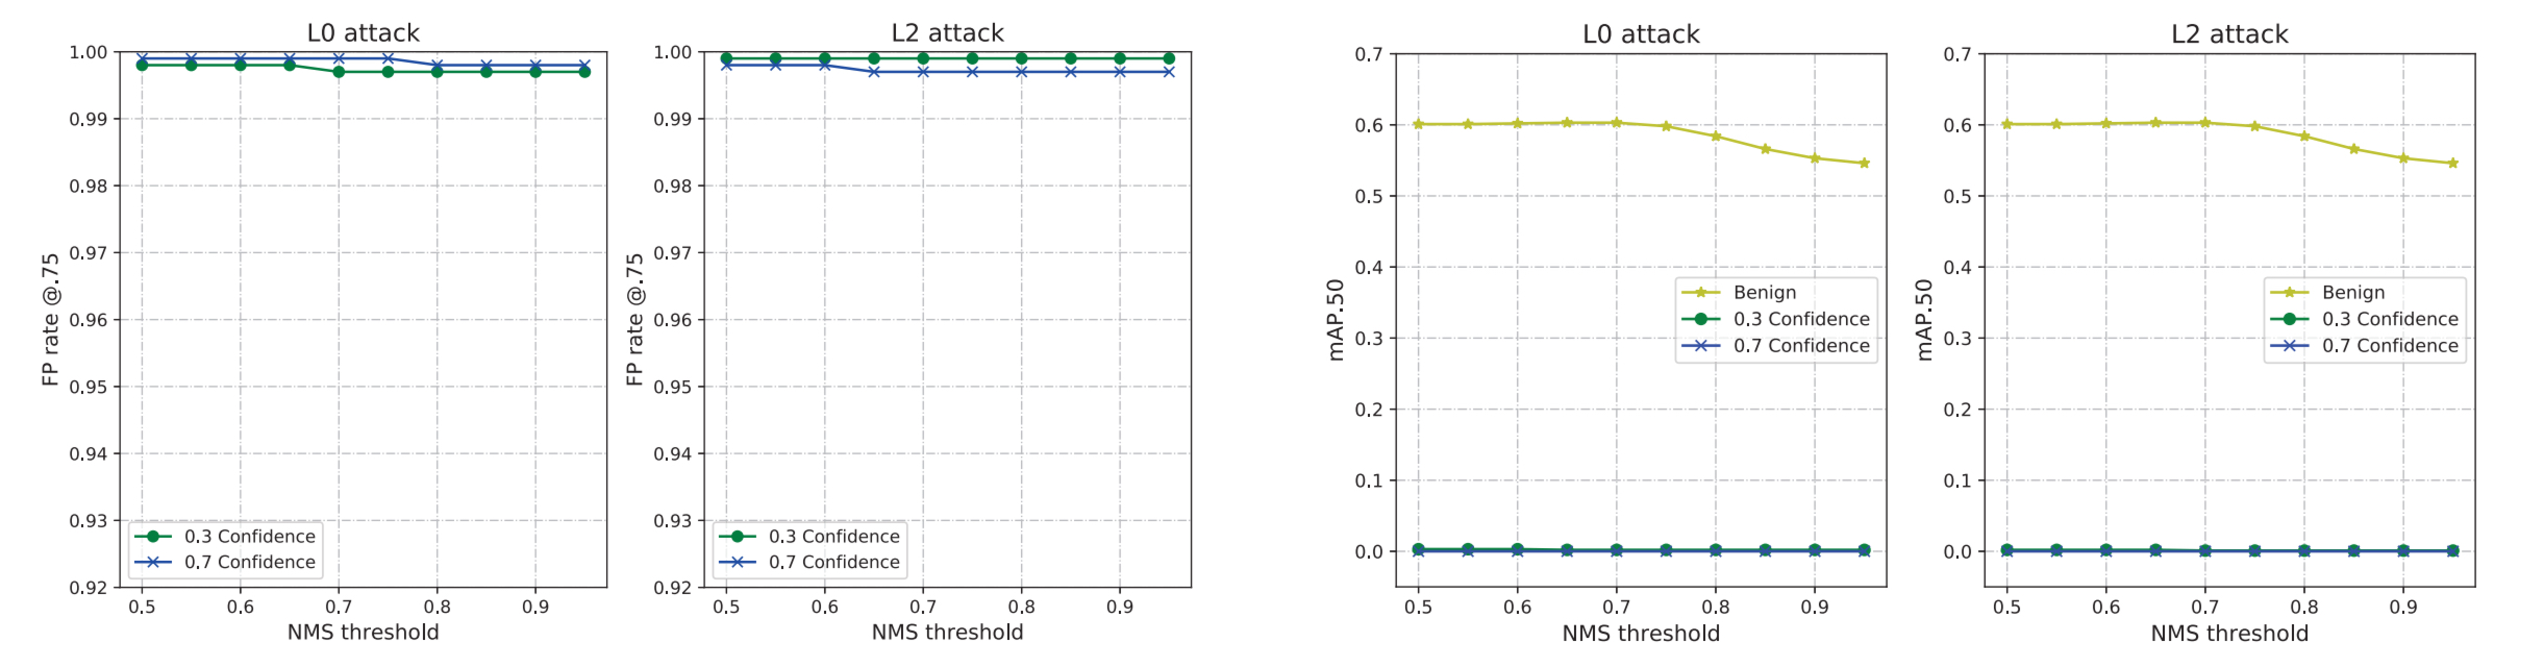
\includegraphics[width=16.0cm]{figures/daedalus-result-fp-map.pdf}
\end{center}
\caption{
モデルは YOLO-v3 で MSCOCO2017 validation データから 100 枚サンプリングして提案手法を検証した結果.
左の二つが FP rate を測定したもので, 右の二つが mAP を測定したものであり, 横軸はどちらも NMS の閾値である.
右の二つの結果は mAP の IoU の IoU 閾値として 0.5 を用いており, 黄色い線の benign は clean データに対する結果である.
図は \cite{wang2019daedalus} より引用.
}
\label{fig:daedalus-result-fp-map}
\end{figure}
%
%
\begin{figure}[htbp]
\begin{center}
\includegraphics[width=10.0cm]{figures/daedalus-example.pdf}
\end{center}
\caption{
YOLO-v3 に対する攻撃の例.
大量の bbox が誤検出されている.
摂動は拡大すれば目視で確認できなくはないというレベルになっている.
図は \cite{wang2019daedalus} より引用.
}
\label{fig:daedalus-example}
\end{figure}
%

bbox を検出するという処理は detector にとって常に必要なものであり, この論文では adversarial examples の作成を複数モデルのアンサンブルで実施することで, どのモデルに対しても攻撃が成功することも示している.
このアンサンブルは単純に loss の計算を複数モデルの平均にするだけでよい.
detector としてよく使われるものはそれほど種類が多くはないため, アンサンブルによってかなり広範囲を攻撃対象とできる可能性がある.
この手法は digital attack で摂動も画像全体に適用するものであるため, このままでは自動運転などの脅威にはならないが, 方向性として bbox を攻撃するという手法があることを認識しておくことは重要かもしれない.

この手法は, detector の bbox 検出部分に注目して大量の bbox を誤検出させるアルゴリズムを考案したという点が興味深い.
これまでは detector に対する攻撃手法は classifier に対する攻撃手法を拡張するというものが多かったため, detector に対する攻撃に新たな視点をもたらしている.
detector に対する攻撃が様々な観点から進展していくことで, detector の性質がより深く理解されることが期待される.

\clearpage
\section{防御手法の各論}
\label{sec:defenses}
各防御手法について解説する.
様々なアイデアを駆使する防御手法の中から, 重要性や汎用性が高そうな手法を中心に, 図 \ref{fig:defense-process} の各プロセスに該当する手法を選出した.
解説する論文の一覧は図 \ref{fig:defense-summary-table} の通りであり, この章では各手法について詳しく解説していく.
%
\begin{figure}[htbp]
\begin{center}
\includegraphics[width=16.0cm]{figures/defense-summary-table.pdf}
\end{center}
\caption{
本書で解説する防御手法の一覧とその特徴をまとめた表.
基本戦略, 使用する外部リソース, 対応コスト, という観点でまとめている.
対応コストは定量的なものではなく, 該当手法の導入に人手の作業がどれくらい発生するかと推論速度への影響がどれくらいかを大まかに評価したものになっていることに注意されたい.
文字が小さいため拡大して見ることを推奨.
}
\label{fig:defense-summary-table}
\end{figure}
%



\subsection{Explaining and Harnessing Adversarial Examples}
\label{subsec:explaining-and}
%
\begin{table}[htbp]
\begin{center}
\begin{tabular}{|c|c|}
\hline
分類の観点 & この手法が該当するもの \\
\hline
基本戦略 & 正則化 \\
使用する外部リソース & adversarial examples \\
対応コスト & 人的コスト:中, 推論コスト:小 \\
\hline
\multicolumn{2}{|c|}{非公式実装: 検証実験のコードに含まれている} \\
\hline
\end{tabular}
\label{tb:explaining-and-summary}
\end{center}
\end{table}
%

FGSM を提案した論文 \cite{goodfellow2014explaining} において、防御方法である adversarial training も同時に提案されている。
アイデアとしては straightforward で, モデルが adversarial examples に対して誤認識をしてしまうならば, その adversarial examples を学習データに含めて学習すればよいという方針である.
これを実現するには何かしらの攻撃手法を導入して adversarial examples を作成する必要があり, その攻撃手法に強く依存した防御手法になっている.

基本戦略は正則化であり, clean なデータを用いた場合の loss に加えて adversarial examples に対する loss も合わせた loss を構成する.
そのため通常の学習で使用するリソース以外にも adversarial examples の分だけ余分にリソースが必要となる.
adversarial examples を作成しそれを含めて学習し直す必要があるので人的コストは中程度掛かるが, 学習後のモデルは adversarial training の有無に依らずに同一なので推論に必要となる余分なコストは発生しない.

定式化は上で述べたことをそのまま実行するだけで, 以下の loss function で学習をすればよい(ここでは単一のデータでの loss function として書いているが, 実際の学習ではミニバッチを使用する).
%
\begin{eqnarray}
\tilde{J} (f, x, y) = \alpha J (f, x, y_{\text{true}}) + (1 - \alpha) J (f, x + \omega, y_{\text{true}}).
\label{eq:explaining-and-loss}
\end{eqnarray}
%
元論文では $\alpha = 0.5$ と $\omega$ を作成する際に FGSM を使用している.
$\omega$ を作成する際には状況に応じて様々な攻撃手法を採用することが可能である

実験は MNIST を用いて実施しており, maxout network \cite{goodfellow2013maxout} に対して $\epsilon = 0.25$ の adversarial examples を作成し, adversarial training なしでは誤認識率が 89.4\% だったが adversarial training ありでは 17.9\% まで減少したと報告されている.

この adversarial training は広く使われている防御手法であるが, \cite{kurakin2016adversarial} で label leaking という問題点が指摘された.
これは少し混乱しやすいので順を追って見ていこう.
まず $f_{\text{label}} (x) \neq y_{\text{true}}$ というデータ $x$ を考える.
この $x$ に対応する $x_{\text{adv}}$ を作成して adversarial training を実施すると, $x$ は当てられなくとも $x_{\text{adv}}$ は当てられるという傾向を持ったモデルが構築され得る.
これはモデルとしては対象物の特徴を捉えるというより摂動のみに注目して予測をするという振る舞いをしてしまうため, テストデータを評価する際に clean なデータは当てられないが adversarial examples は当てやすいという状況を生んでしまう.
そのため, 不当に adversarial examples に対する精度を高めてしまうので正しい評価ができない, という問題である.

この label leaking を防ぐには, 学習の際に $y_{\text{true}}$ を使うのではなく $f_{\text{label}} (x)$ を使えばよい.
これを考慮した loss function は以下のように書ける.
%
\begin{eqnarray}
\tilde{J} (f, x, y) = \alpha J (f, x, y_{\text{true}}) + (1 - \alpha) J (f, x + \omega, f_{\text{label}} (x)).
\label{eq:explaining-and-loss-model-prediction}
\end{eqnarray}
%
これは学習時の話であり, テスト時に adversarial examples を作成するときは $y_{\text{true}}$ を使用すればよい.



\subsection{Distillation as a Defense to Adversarial Perturbations against Deep Neural Networks}
\label{subsec:distillation-as}
%
\begin{table}[htbp]
\begin{center}
\begin{tabular}{|c|c|}
\hline
分類の観点 & この手法が該当するもの \\
\hline
基本戦略 & 外部リソース使用 \\
使用する外部リソース & student network \\
対応コスト & 人的コスト:大, 推論コスト:小 \\
\hline
\multicolumn{2}{|c|}{非公式実装: \href{https://github.com/carlini/nn_robust_attacks}{https://github.com/carlini/nn\_robust\_attacks}} \\
\hline
\end{tabular}
\label{tb:distillation-as-summary}
\end{center}
\end{table}
%

これは \cite{papernot2016distillation} によって提案された手法であり, 蒸留を用いて構築した student network は元のモデルに対する adversarial examples に対して誤認識率が低いということを示した.
蒸留とは図 \ref{fig:distillation-as-summary} のように元のモデル(teacher network と呼ぶ)の出力を用いて蒸留されたモデル(student network と呼ぶ)を学習する手法を指す.
この論文で考えている状況は, 元の学習モデルの情報は攻撃者も知ることができて adversarial examples を作成するが, student network は防御者のみが扱えるもので, この student network は teacher network を基に作成した adversarial examples に対して誤認識しづらいという結果が得られている.
%
\begin{figure}[htbp]
\begin{center}
\includegraphics[width=14.0cm]{figures/distillation-as-summary.pdf}
\end{center}
\caption{
蒸留の概念図.
元のモデルの出力を蒸留されたモデルの入力にして学習をする.
この図での $F(X)$ は本書での表記における $f_{\text{prob}}(x)$ に対応している.
図は \cite{papernot2016distillation} より引用.
}
\label{fig:distillation-as-summary}
\end{figure}

基本戦略は外部リソース使用であり, 元のモデルとは独立の student network を準備してそれを学習する必要がある.
student network のアーキテクチャ設計や再学習に係るパラメタ調整など人的コストは大きい.
一方で, 典型的には student network は元のモデルよりも小さく作ることが多いため, 推論のコストは低く, 場合によっては元のモデルよりも速い推論速度を達成し得る.

蒸留自体は adversarial examples とは独立の概念であるため, 詳しくは \cite{hinton2015distilling} などを参照してもらうとして, ここでは蒸留の際に重要となる温度パラメタについて解説をする.
温度パラメタ $T$ とは softmax 値を計算する際に出力確率値がなだらかになるように導入するパラメタである.
%
\begin{eqnarray}
f_{\text{prob}, i} (x) = \frac{e^{f_{\text{logit}, i}(x) / T}}{\sum_{i' = 1}^{C} e^{f_{\text{logit}, i'}(x) / T}}.
\label{eq:distillation-as-temp}
\end{eqnarray}
%
ここでは成分の計算が陽に見えるように $i$ 番目の成分を $f_{\text{prob}, i} (x)$ などと表記している.
この温度パラメタ $T$ が大きいほどクラス毎の確率値の差が小さくなり, より soft な出力になる(T が無限大の極限を取ればどのクラスの出力も $1 / C$ となる).
温度パラメタの導入により, 温度が高い場合に入力の微小な変化の影響を受けづらいという定性的な議論が展開される.
これは $\partial f_{\text{prob}, i} (x) / \partial x_j$ という微分を考えた時に logit が $1/T$ 倍されているので温度パラメタを導入しない場合と比べて変化量が小さくなるためである.
ただし通常は推論時には $T=1$ とするため, ここでの議論は「定性的」であり, 論文でも future work としている.

提案手法は, $T$ を導入して元のモデルを学習した後に $(x, f_{\text{prob}} (x))$ を作成し, それを入力として student network を学習する, というのみである.
student network を $f^d$ と書くことにすると, loss function は以下のようになる.
%
\begin{eqnarray}
J(f, f^d, x) = \sum_{i = 1}^{C} f_{\text{prob}, i} (x) \log f^d_{\text{prob}, i} (x).
\label{eq:distillation-as-loss}
\end{eqnarray}
%

MNIST と CIFAR10 を用いた実験結果に移る.
モデルはそれぞれのデータセットに対して特に工夫を凝らしていない CNN を構築しており, adversarial examples は \cite{papernot2016limitations} で提案された saliency map を使った手法で作成する.
結果は図 \ref{fig:distillation-as-result-table} で, $T$ を高く設定することで誤認識率を減少させることに成功している.
%
\begin{figure}[htbp]
\begin{center}
\includegraphics[width=16.0cm]{figures/distillation-as-result-table.pdf}
\end{center}
\caption{
温度パラメタ $T$ と adversarial examples の攻撃成功率の関係性.
$T$ を大きくするほど攻撃成功率が下がり, 防御が成功していることを示している.
図は \cite{papernot2016distillation} より引用.
}
\label{fig:distillation-as-result-table}
\end{figure}
%

また, 図 \ref{fig:distillation-as-diff} にあるように clean データに対する性能の変化も 1.5\% 以内であることも報告している.
MNIST ではどれも精度が下がっているが CIFAR10 では逆に精度が上がる場合もあるため, 蒸留をしたり $T$ を高くすることで必ずしも精度が下がるわけではないことが示されている.
%
\begin{figure}[htbp]
\begin{center}
\includegraphics[width=8.0cm]{figures/distillation-as-diff.pdf}
\end{center}
\caption{
蒸留の前後で clean データに対する精度変化を調べた結果.
図は \cite{papernot2016distillation} より引用.
}
\label{fig:distillation-as-diff}
\end{figure}

論文では student network が元のモデルに統計的に近しいことなども議論しているが, 本質的に adversarial examples とは関係がないのでここでは割愛する.

この論文は蒸留を adversarial examples の防御として利用するという点で興味深いが, 状況として攻撃者は元のモデルの情報は取得できるが student network の情報は取得できないという特殊な想定をしている点に注意が必要である.
例えば, inception-v3 \cite{szegedy2016rethinking} のようなよく知られたモデルをそのまま使う場合は攻撃の危険に晒される可能性があり, それを防ぐためにこの手法が利用する, というような使い方が考えられる.



\subsection{On Detecting Adversarial Perturbations}
\label{subsec:on-detecting}
%
\begin{table}[htbp]
\begin{center}
\begin{tabular}{|c|c|}
\hline
分類の観点 & この手法が該当するもの \\
\hline
基本戦略 & 外部リソース使用 \\
使用する外部リソース & binary classifier \\
対応コスト & 人的コスト:中, 推論コスト:大 \\
\hline
\multicolumn{2}{|c|}{非公式実装: \href{https://github.com/carlini/nn_robust_attacks}{https://github.com/carlini/nn\_robust\_attacks}} \\
\hline
\end{tabular}
\label{tb:on-detecting-summary}
\end{center}
\end{table}
%

これは \cite{metzen2017detecting} によって提案された手法であり, 元のモデルとは別の adversarial examples か否かを二値分類する binary classifier を準備するというものである.
図 \ref{fig:on-detecting-model} のように, 元のモデルと同じ入力もしくは元のモデルの中間層出力を binary classifier の入力とする.
FGSM などの基本的な攻撃手法に対して, 元のモデルでは誤認識を引き起こす adversarial examples に対して検出を試み, binary classifier の勾配情報も攻撃者に使われた状況でも探索範囲内の worst case でも 70\% 以上検出できることを示した(二値分類で chance rate が 50\% なので非常に高いというわけではない).
%
\begin{figure}[htbp]
\begin{center}
\includegraphics[width=14.0cm]{figures/on-detecting-model.pdf}
\end{center}
\caption{
元のモデルと binary classifier (論文では Adversarial Detector で AD と表記しているが, object detection との混同が生じやすいので本書では binary classifier と表記する) を併用している図.
元のモデルは ResNet を使用しており, Conv は convolution, Res は residual blocks, GAP は global average pooling, Dens は fully connected を意味している.
binary classifier は比較的シンプルなモデルで, 入力として元のモデルと同じ入力や元のモデルの中間層を使う(どれが良いかは実験で決める).
また, MP は max pooling である.
図は \cite{metzen2017detecting} より引用.
}
\label{fig:on-detecting-model}
\end{figure}

基本戦略は外部リソース使用であり, 元のモデルとは独立の binary classifier を準備してそれを学習する必要がある.
binary classifier の設計や学習が必要となるが, モデルはあまり複雑ではないので人的コストは中程度である.
推論時には元のモデルの予測とは別に binary classifier の予測が必要になるため推論コストは大きい(特に元のモデルの中間層出力を使用する場合は中間層出力を得るまでは並列で走らせることもできない).

導入した binary classifier を clean データとその adversarial examples をそれぞれラベル 0, 1 として学習すればよいだけなので, 手法としてはシンプルである.
論文では状況設定として static adversaries と dynamic adversaries を考えており, 前者は攻撃者が元のモデルの情報だけを取得できる場合で後者は binary classifier の情報も取得できる場合としている.
前者は元のモデルの勾配情報を作って adversarial examples を作成すればよいだけで, 後者は binary classifier の勾配情報も用いて adversarial examples を作成する必要がある.
後者に関しては $x_{\text{adv}}$ を adversarial examples ではなく clean データと誤認識させたいので, $x_{\text{adv}}$ ありきでそれをラベル 1 ではないという方向の摂動を作りたいという問題設定になる.
そのため, I+FGSM のように $x_{\text{adv}}$ を逐次的に構成していく方法を念頭に置いており, 以下のように書ける. 
%
\begin{eqnarray}
x_{\text{adv}}^{(t+1)} = \text{clip} ( &&x_{\text{adv}}^{(t)} + \alpha \left[ (1 - \sigma) \cdot \text{sign} \left( \Delta_x J(f, x_{\text{adv}}^{t}, y_{\text{true}}) \right) + \sigma \cdot \text{sign} \left( \Delta_x J(f_{\text{b}}, x_{\text{adv}}^{t}, 1) \right) \right] \nonumber \\
&&, x - \omega, x + \omega ).
\label{eq:on-detecting-adv}
\end{eqnarray}
%
ここで, binary classifier として $f_b$, $\alpha = 0.25$, 元のモデルと binary classifier の寄与を調整するパラメタ $0 \leq \sigma \leq 1$ が導入されている.

実験には CIFAR10 データを用いており, adversarial examples の作成方法として FGSM, I+FGSM, DeepFool を用いている.
まず, static adversaries の結果は図 \ref{fig:on-detecting-static} の通りである.
adversarial examples を使わずに予測させた結果は期待通り 50\% 程度であり, adversarial examples に対しては概ね 80\% 以上の検出率を達成している.
大まかな傾向としては元のモデルを誤認識させやすい adversarial examples ほど binary classifier で検出しやすくなっている.
binary classifier の入力としては元のモデルの入力と出力の中間に位置する中間層出力を使うのが良いという結果が示されている.
これはなかなか解釈が難しいが, モデル依存性が大きいようにも思われる.
%
\begin{figure}[htbp]
\begin{center}
\includegraphics[width=14.0cm]{figures/on-detecting-static.pdf}
\end{center}
\caption{
static adversaries 実験の結果.
左図は縦軸が binary classifier による adversarial examples の検出成功率で, 横軸が元のモデルによる adversarial examples の予測精度である.
$l_{\infty}$ ノルムの上限 $\epsilon$ 様々に変えた結果がプロットされており, 印が左側にいくほど $\epsilon$ が大きい.
右図は縦軸は同じで横軸は binary classifier の入力としてどの情報を使うかである.
図は \cite{metzen2017detecting} より引用.
}
\label{fig:on-detecting-static}
\end{figure}


次に, dynamic adversaries の結果は図 \ref{fig:on-detecting-dynamical-exp} の通りである.
こちらの場合 binary classifier の勾配情報も利用して adversarial examples を作成しているため検出成功率は低下しているが, dynamic では worst case でも 70\% 以上の検出成功率を達成している.
$\sigma$ の値が小さいときは $x_{\text{adv}}$ として元のモデルの勾配情報を重く扱っている場合で, 元のモデルをうまく騙せるものになっているが, その場合 binary classifier で検出しやすくなる.
一方で $\sigma$ の値が大きいときは $x_{\text{adv}}$ として binary classifier の勾配情報を重く扱っている場合で, 元のモデルをうまく騙せなくなっていることに加えて binary classifier での検出成功率も高く保たれているという点は興味深い.
モデルの誤認識率を高めるようにすれば binary classifier で検出しやすくなり, binary classifier を騙そうとし過ぎると元のモデルで誤認識しないばかりか binary classifier を騙すこともできなくなることを示している\footnote{
この部分は自明ではない.
binary classifier に特化するとナイーブには binary classifier を騙しやすい $x_{\text{adv}}$ が作成できるはずだが, 単純な binary classifier では摂動が限定的になってしまって騙しきれないのかもしれないが, 著者はよく知らない.
}.
%
\begin{figure}[htbp]
\begin{center}
\includegraphics[width=8.0cm]{figures/on-detecting-dynamical-exp.pdf}
\end{center}
\caption{
dynamic adversaries の実験結果.
縦軸は binary classifier による adversarial examples の検出成功率で, 横軸が元のモデルによる adversarial examples の予測精度である.
パラメタ $\sigma$ を $0.1$ 刻みで $[0.0, 1.0]$ の範囲で動かした結果であり, $\sigma$ の値が小さいほど左側の点になる.
青い点は binary classifier の学習に binary classifier の勾配情報を使ってないもので, 赤い点は binary classifier の勾配情報を使ったものである.
$\epsilon = 1 / 255$ で I+FGSM で adversarial examples を作成している.
図は \cite{metzen2017detecting} より引用.
}
\label{fig:on-detecting-dynamical-exp}
\end{figure}

この手法は binary classifier という元のモデルと独立なモデルの導入による防御方法で, adversarial training や元のモデルの中間層の情報を使う場合はそこが密結合となってしまうが, 方向性としては元のモデルとは独立に別のモデルを準備する方向のため導入や削除やアップデートがしやすくなる.
計算資源の面ではコストも低くはないが, 実運用上の方向性しては有望な方向性の一つであろう.



\subsection{MagNet: a Two-Pronged Defense against Adversarial Examples}
\label{subsec:magnet}
%
\begin{table}[htbp]
\begin{center}
\begin{tabular}{|c|c|}
\hline
分類の観点 & この手法が該当するもの \\
\hline
基本戦略 & 外部リソース使用 \\
使用する外部リソース & (複数の) AutoEncoder \\
対応コスト & 人的コスト:中, 推論コスト:大 \\
\hline
\multicolumn{2}{|c|}{公式実装: \href{https://github.com/Trevillie/MagNet}{https://github.com/Trevillie/MagNet}} \\
\hline
\end{tabular}
\label{tb:magnet-summary}
\end{center}
\end{table}
%

これは \cite{meng2017magnet} によって提案された手法であり, 図 \ref{fig:magnet-summary} のようにまずは(一般に複数の)検出器で入力データが adversarial examples か否かを分類し, adversarial examples と分類されなかったものは reformer で正常なデータに近づくように変換して classifier で予測する二段階の仕組みになっている.
検出器の段階では clean なデータから大きく離れる adversarial examples を検出し, それをすり抜けてくる小さな変化量の adversarial examples に対しては clean なデータに戻るように変換をすることで正しい予測をするという戦略となっている.
最も簡単な場合としては, 検出器として AutoEncoder を用いて再構成誤差に閾値を設定して最初の検出を実施し, それをくぐり抜けたデータは同じ AutoEncoder で再構成したデータを入力に予測を実施する.
%
\begin{figure}[htbp]
\begin{center}
\includegraphics[width=10.0cm]{figures/magnet-summary.pdf}
\end{center}
\caption{
Magnet の概要.
入力データはまず検出器で adversarial examples か否かを分類される.
adversarial examples ではないと分類されたデータは reformer で clean データのサンプルに近づくように変換されるため, 検出器をすり抜けた adversarial examples も正しいラベルと認識されやすくなり, clean データに対しても影響少なく予測できる.
図は \cite{meng2017magnet} より引用.
}
\label{fig:magnet-summary}
\end{figure}


検出器は入力データに対して adversarial examples か否かを分類するものとなり, 一般にはどのようなモデルでもよい.
この論文では後の reformer への使い回しも考慮して, 典型的なものとして AutoEncoder を用いている.
学習は clean データに対する再構成誤差を小さくすることを目的とするため, 以下の loss function を設定する.
%
\begin{eqnarray}
J(AE, x) = \| x - AE(x) \|_2.
\label{eq:magnet-ae-train}
\end{eqnarray}
%
ここで, $AE$ は AutoEncoder であり Encoder のあとに Decoder を適用して $x$ を再構成するものである.
学習した AutoEncoder は推測時には $\|x - AE(x)\|_p$ を計算することで adversarial examples の検出に利用することが可能で, 閾値としては clean データが adversarial examples と分類されてしまう false positive の割合が一定値以下になるように設定する(学習や閾値設定には adversarial examples を用いない).

検出器をもう少し発展させて予測モデルの logit 出力に対する $x$ と $AE(x)$ の divergence を用いるということもできる.
adversarial examples は $x$ の空間では近くても $f_{\text{logit}} (x)$ の空間では遠いものなので, それを利用するアプローチである.
logit から softmax 値を計算して確率値として, 以下のように Jensen-Shannon divergence を計算する.
%
\begin{eqnarray}
JSD(f_{\text{prob}} (x)\|f_{\text{prob}} (AE(x))) &=& \frac{1}{2} D_{KL} \left(f_{\text{prob}} (x) \| \frac{f_{\text{prob}} (x) + f_{\text{prob}} (AE(x)) }{2} \right) \nonumber \\
&+& \frac{1}{2} D_{KL} \left(f_{\text{prob}} (AE(x)) \| \frac{f_{\text{prob}} (x) + f_{\text{prob}} (AE(x)) }{2} \right).
\label{eq:magnet-jsd-ae}
\end{eqnarray}
%
ここで $D_{KL}$ は Kullback-Leibler divergence である.
これも分類時には閾値が必要となるが, 先ほどと同じように clean データのみを用いて false positive が一定値以下になるように定める.
$x$ と $AE(x)$ それぞれの softmax 値が同じ最大要素のみでほぼ 1 になると $JSD$ の値は 0 に近づき違いが見えづらくなるため, 数値的なテクニックとして式 \ref{eq:distillation-as-temp} と同様に温度パラメタを導入する.

一方で reformer としても AutoEncoder を使用する.
これも clean データの再構成誤差で学習し, 一段目の検出器をすり抜けてきた adversarial examples を clean なデータ分布のサンプルとして再構成する方向に働くため, それを classifier の入力とすることで正しい予測が得られると期待される.

実験は MNIST と CIFAR10 で実施している.
予測モデルは特に変わったところのない convolution と ReLU と max pooling や gloval average pooling のモデルのためここでは説明は割愛する.
検出器や reformer は MNIST に関しては図 \ref{fig:magnet-mnist} のように構成していて検出器を 2 つ準備しており\footnote{
MNIST は簡単なデータセットであるため CIFAR10 のように 1 つの検出器と reformer でよい気がするが, なぜ検出器を 2 つ準備しているのかは著者は知らない.
}, CIFAR10 に関しては図 \ref{fig:magnet-cifar10} のように構成している\footnote{
CIFAR10 は decoder の最後の convolution のチャンネル数が 1 になっているが, これは論文の誤植で 3 だと思われる.
}.
検証のための adversarial examples の作成手法としては, FGSM, I+FGSM, Deepfool, Carlini の方法\footnote{
これは loss function を設定してそれに基づいて摂動を求める手法で, 以下の loss function を用いる.
%
\begin{eqnarray}
\min_{\omega} \left[ \|\omega\|_p + c \cdot \max (f_{\text{logit}, y_{\text{true}}} (x_{\text{adv}}) - \max (\{ f_{\text{logit} (x_{\text{adv}}), i} : i \neq y_{\text{true}} \}), - \kappa) \right].
\label{eq:magnet-adv-cw}
\end{eqnarray}
%
さらに $x + \omega \in [0, 1]^m$ となるよう制限する.
これは正しいラベルの logit の値がそれ以外の logit で最大値のものと比べて十分小さくなるように摂動を作成するもので, それだけを目的にするとモデルに特化しすぎて transferability が低くなるため $- \kappa$ で制限している.
FGSM とは異なりこの loss を用いて optimizer を用いて最適化することで所望の摂動を得る.
}, \cite{carlini2017towards} を用いている.
%
\begin{figure}[htbp]
\begin{center}
\includegraphics[width=10.0cm]{figures/magnet-model-mnist.pdf}
\end{center}
\caption{
MNIST に対する検出器と reformer の構成.
検出器は 2 つ準備している.
convolution は出力後に入力サイズと同じになるように padding する.
図は \cite{meng2017magnet} より引用.
}
\label{fig:magnet-mnist}
\end{figure}
%
\begin{figure}[htbp]
\begin{center}
\includegraphics[width=6.0cm]{figures/magnet-model-cifar10.pdf}
\end{center}
\caption{
CIFAR10 に対する検出器と reformer の構成.
同一の AutoEncoder を用いている.
convolution は出力後に入力サイズと同じになるように padding する.
図は \cite{meng2017magnet} より引用.
}
\label{fig:magnet-cifar10}
\end{figure}


MNIST の結果は図 \ref{fig:magnet-result-mnist} の通りである.
検出器は Jansen-Shannon divergence は用いずに再構成誤差のみを用いており, 閾値としては validation セットに対する false positive が 0.1\% になるように定めている.
CW の方法では元のモデルでは全く正答することができていないが, MagNet によって 90\% を超える精度を達成している.
また, clean テストデータに対しては MagNet なしでは 99.4\% であり MagNet ありでは 99.1\% であり影響が少ないことが示されている.
%
\begin{figure}[htbp]
\begin{center}
\includegraphics[width=10.0cm]{figures/magnet-result-mnist.pdf}
\end{center}
\caption{
防御手法の有無による MNIST のテストデータに対する精度の違い.
精度は clean データに対して正答することができるものがを adversarial examples に差し替えた場合の精度を示している.
防御手法のうち検出器は Jansen-Shannon divergence は用いずに再構成誤差のみを用いている.
攻撃は予測モデルの情報だけを使える状況設定で MagNet に対する情報は用いていない.
図は \cite{meng2017magnet} より引用.
}
\label{fig:magnet-result-mnist}
\end{figure}
%

CIFAR10 の結果は図 \ref{fig:magnet-result-cifar10} の通りである.
検出器は再構成誤差だけではなく Jansen-Shannon divergence も用いており, 温度パラメタは $T=10, 40$ の 2 つの場合を併用している.
MNIST と比べるとうまく防御できない場合が増えているが, それでもMagNet によって 75\% を超える精度を達成している.
ただし, clean テストデータに対しては MagNet なしでは 90.6\% であり MagNet ありでは 86.8\% であり若干の影響が出ている.
%
\begin{figure}[htbp]
\begin{center}
\includegraphics[width=10.0cm]{figures/magnet-result-cifar10.pdf}
\end{center}
\caption{
防御手法の有無による CIFAR10 のテストデータに対する精度の違い.
精度は clean データに対して正答することができるものがを adversarial examples に差し替えた場合の精度を示している.
防御手法のうち検出器は再構成誤差と $T=10, 40$ の場合の Jansen-Shannon divergence を併用している.
攻撃は予測モデルの情報だけを使える状況設定で MagNet に対する情報は用いていない.
図は \cite{meng2017magnet} より引用.
}
\label{fig:magnet-result-cifar10}
\end{figure}
%

この手法は検出器と reformer という 2 つの組み合わせで防御性能を高めたものであるが, 特に reformer で入力画像を clean データ分布に近いものに変換するという考えが興味深いものであった.
この手法以降, 様々な方法で adversarial examples の摂動の効果を除去して正しく予測できるようにする研究が発展した.
ただし, 入力画像の変更は clean データの場合にモデルの degradation を引き起こす恐れもあるので注意が必要である.



\subsection{PixelDefend: Leveraging Generative Models to Understand and Defend against Adversarial Examples}
\label{subsec:pixeldefend}
%
\begin{table}[htbp]
\begin{center}
\begin{tabular}{|c|c|}
\hline
分類の観点 & この手法が該当するもの \\
\hline
基本戦略 & 外部リソース使用 \\
使用する外部リソース & PixelCNN \\
対応コスト & 人的コスト:中, 推論コスト:大 \\
\hline
\multicolumn{2}{|c|}{公式実装: \href{https://github.com/microsoft/PixelDefend}{https://github.com/microsoft/PixelDefend}} \\
\hline
\end{tabular}
\label{tb:pixeldefend-summary}
\end{center}
\end{table}
%

これは \cite{song2017pixeldefend} によって提案された手法であり, 元のモデルとは別の clean データで pre-train された pixelCNN を導入し, 入力データを purify することで摂動の効果を弱めて誤認識を防ぐ.

基本戦略は外部リソースの使用で, pixelCNN を用いる.
別のモデルを準備しなければならないので人的コストは中程度で, 推論は先に pixelCNN を通してから元の予測モデルを適用するのでコストは大きい.

pixelCNN \cite{oord2016pixel, salimans2017pixelcnn++} は画像用に考案された tractable な尤度を基にした生成モデルである.
同時確率分布は以下のように定義される.
%
\begin{eqnarray}
p_{\text{CNN}} (x) = \prod_{i} p_{\text{CNN}} (x_i | x_{1:i-1}).
\label{eq:pixeldefend-pixelcnn-joint-distrib}
\end{eqnarray}
%
これを $- \log \left( p_{\text{CNN}} (x) \right) / (m \times \log 2)$ としたものを bits per dimension と呼び, モデルの評価によく用いられる.
ここではかなり簡略化して書いてあるが, 実際には未来方向の情報を mask した convolution を使ってコンテキストを取得して未来方向のピクセルを予測していく.
pixelCNN は予測するピクセルを softmax 値を用いて選択するモデルになっているため, どのピクセル値がどれくらいの確率であるかが tractable になっているため, 入力データを実現する同時確率が計算可能である.

すなわち clean データで学習した pixelCNN があれば, 入力データの同時確率を計算することでその確率が高ければ clean データで低ければ adversarial examples であると分類できる.
これは統計的な枠組みで議論できる.
clean データ $x^{(1)}, x^{(2)}, \dots x^{(N)}$ を iid で確率分布 $p (\mathcal{X})$ からサンプルされたものだとする.
対象となるデータ $x_{\text{adv}}$ が iid で確率分布 $p (\mathcal{X_{\text{adv}}})$ からサンプルされたものだとして, 帰無仮説として $p (\mathcal{X}) = p (\mathcal{X_{\text{adv}}})$ を採用して対立仮説として $p (\mathcal{X}) \neq p (\mathcal{X_{\text{adv}}})$ を採用する.
統計量 $T$ を以下のように定義する.
%
\begin{eqnarray}
T = T(x_{\text{adv}}; x^{(1)}, x^{(2)}, \dots x^{(N)}) = \sum_{i=1}^{N} \mathbb{I} \left[ p_{\text{CNN}} (x^{(i)}) \leq p_{\text{CNN}} (x_{\text{adv}}) \right].
\label{eq:pixel-defend-pixelcnn-test-stat}
\end{eqnarray}
%
ここで $\mathbb{I} [\cdot]$ は indicator function で括弧内の条件が true なら 1 でそうでなければ 0 を返す.
あとは $T^{(i)} = T(x^{(i)}; x^{(1)}, \dots, x^{(i-1)}, x_{\text{adv}}, x^{(i+1)}, \dots, x^{(N)})$ として permutation test を実施すればよい.
具体的には p 値が以下で計算される.
%
\begin{eqnarray}
p = \frac{1}{N + 1} \left( \sum_{i=1}^{N} \mathbb{I} [T_i \leq T] + 1 \right) = \frac{T + 1}{N + 1}.
\label{eq:pixel-defend-pixelcnn-test-pvalue}
\end{eqnarray}
%

以上が adversarial examples を検出する仕組みであったが, もう一歩進めて pixelCNN を入力データを purify するために用いて正しい予測を実施するという手法も提案されている.
これは clean データで学習した pixelCNN が出力として clean データの分布に従うピクセル値を出力しやすいという性質を利用したもので, アルゴリズム \ref{alg:pixeldefend-alg} にその手順を示す.
%
\begin{algorithm}
\caption{pixelCNN によるデータ purification のアルゴリズム}
\label{alg:pixeldefend-alg}
\begin{algorithmic}[1]
    \State Input: 入力データ $x$, パラメタ $\epsilon_{\text{defend}}$, 学習済みの pixelCNN $p_{\text{CNN}}$.
    \State Output: purify されたデータ $x_{\text{purified}}$.
	\State 出力を初期化: $x_{\text{purified}} \leftarrow x$
	\For {各ピクセル $x_i \in \mathcal{X}$}
	\State 出力範囲を設定: $R \leftarrow \left[ \max (x_i - \epsilon_{\text{defend}}, 0), \min (x_i + \epsilon_{\text{defend}}, 255) \right]$.
	\State $x_{\text{purified}, i}$ に対応する pixelCNN の出力を計算: $o = \prod_{i'}^i p_{\text{CNN}} (x_{\text{purified}, i'} | x_{\text{purified}, 1:i' - 1})$.
	\State $x_{\text{purified}}$ の要素を更新: $x_{\text{purified}, i} \leftarrow \argmax_{z \in R} \left[ o[z] \right]$.
    \EndFor
\end{algorithmic} 
\end{algorithm}
%

実験は CIFAR10 で実施しており, 攻撃方法は RAND, FGSM, I+FGSM, DeepFool, CW の方法, を用いている.
p 値の分布は図 \ref{fig:pixeldefend-pvalue} で, 画像を purify した例は図 \ref{fig:pixeldefend-purification} である.
どちらも期待通りの挙動を示している.
%
\begin{figure}[htbp]
\begin{center}
\includegraphics[width=14.0cm]{figures/pixeldefend-pvalue.pdf}
\end{center}
\caption{
pixelCNN で CIFAR10 に対して算出した p 値.
BIM は I+FGSM と同一である.
縦軸のスケールは攻撃手法毎に異なる.
図は \cite{song2017pixeldefend} より引用.
}
\label{fig:pixeldefend-pvalue}
\end{figure}
%
\begin{figure}[htbp]
\begin{center}
\includegraphics[width=14.0cm]{figures/pixeldefend-purification.pdf}
\end{center}
\caption{
pixelCNN で CIFAR10 のデータに対して purifaction を実施した例
BIM は I+FGSM と同一である.
画像の下のラベルは clean データで学習した ResNet での予測結果で, purify したデータでは全て正しく予測できている.
図は \cite{song2017pixeldefend} より引用.
}
\label{fig:pixeldefend-purification}
\end{figure}

提案手法の性能を定量的に実験した結果が図 \ref{fig:pixeldefend-cifar10} である.
提案手法は結果が安定していることが読み取れる.
単体では従来手法を上回るほどではないが, 従来手法と組み合わせることで特に性能が高い攻撃手法に対しては adversarial training と比べて良い結果を示している.
また, 組み合わせることで clean data に対する degradation も軽減している.
%
\begin{figure}[htbp]
\begin{center}
\includegraphics[width=14.0cm]{figures/pixeldefend-cifar10.pdf}
\end{center}
\caption{
CIFAR10 のテストデータに対する実験結果.
3 つ数字があるのは adversarial examples として $\epsilon = 2/255, 8/255, 16/255$ それぞれの結果である.
$\epsilon_{\text{defend}} = 16/255$ を用いている.
STRONGEST ATTACK は最も精度が低い攻撃手法の結果である.
Adaptive PixelDefend は $\epsilon_{\text{defend}}$ を攻撃方法に合わせて適した値を手で設定しているものである.
図は \cite{song2017pixeldefend} より引用.
}
\label{fig:pixeldefend-cifar10}
\end{figure}

この手法は pixelCNN を画像の purification に用いたという点が新しいものであった.
MagNet と同様に clean データで学習したモデルを用いて入力データを変換すると adversarial examples が clean データに近づくという性質を利用しており, 他手法と比べることで degradation も抑えられている.
同様のアイデアの手法としては \cite{mustafa2019image} などもある.



\subsection{Mitigating Adversarial Effects Through Randomization}
\label{subsec:mitigating-adversarial}
%
\begin{table}[htbp]
\begin{center}
\begin{tabular}{|c|c|}
\hline
分類の観点 & この手法が該当するもの \\
\hline
基本戦略 & 入力データ変更 \\
使用する外部リソース & なし \\
対応コスト & 人的コスト:小, 推論コスト:中 \\
\hline
\multicolumn{2}{|c|}{公式実装: \href{https://github.com/cihangxie/NIPS2017_adv_challenge_defense}{https://github.com/cihangxie/NIPS2017\_adv\_challenge\_defense}} \\
\hline
\end{tabular}
\label{tb:mitigating-adversarial-summary}
\end{center}
\end{table}
%

これは \cite{xie2017mitigating} によって提案された手法であり, 図 \ref{fig:mitigating-adversarial-summary} のように入力データを小さくリサイズしてから元の画像サイズと同じサイズになるように padding したものを改めて入力データとすることで誤認識を防ぐものである.
%
\begin{figure}[htbp]
\begin{center}
\includegraphics[width=14.0cm]{figures/mitigating-adversarial-summary.pdf}
\end{center}
\caption{
提案手法の概要.
入力データをランダムにリサイズした後, それを一定のサイズになるように 0 padding したものをモデル予測の入力とする.
図は \cite{xie2017mitigating} より引用.
}
\label{fig:mitigating-adversarial-summary}
\end{figure}

基本戦略は入力データ変更で, 摂動の効果が弱まるようにリサイズや 0-padding を用いる.
外部リソースが必要なく, コストが低いのが特徴である.

手法としてはシンプルである.
入力データサイズを [299, 299, 3] の場合を想定しており, まず resize として $rnd \in$ [299, 331) を用いて [$rnd$, $rnd$, 3] とする.
そして 0 埋めした [331, 331, 3] に収まるように resize した画像を配置するというものになっている.
adversarial examples が入力となった場合には, リサイズと 0 padding によって摂動の効果が増幅して誤認識につながることを防ぐというメカニズムである.

実験は, データは ILSVRC2012 の validation セットからランダムにサンプルした 5,000 枚を用いて, adversarial examples の生成は FGSM, DeepFool, CW を用いている.
攻撃対象のモデルは inception-v3, ResNet-v2-101, Inception-ResNet-v2, ens-adv-Inception-ResNet-v2 (ensemble adversarial training と提案手法を併用したもの) としている.
提案手法を導入することによって clean データに対する degradation の可能性が生じるが, 精度劣化は上で紹介したモデルの順に絶対値で 2.7\%, 1.7\%, 0.7\%, 0.8\% でありかなり抑えられている.

まず, 攻撃者が予測モデルの情報だけにアクセスできる場合を考える.
攻撃者はリサイズは 0 padding の存在を知らないため, [299, 299, 3] の入力データを予測モデルの勾配情報を用いて adversarial examples を作成する.
防御側はその adversarial examples をリサイズして 0 padding したものに差し替えて予測する.
その結果が図 \ref{fig:mitigating-adversarial-vanilla} であり, どの攻撃手法に対しても精度が上がっていることが確認できる.
特に DeepFool や CW のように元のモデルに対する攻撃性能が高い手法に対して高い防御性能を発揮している.
これは, FGSM は勾配情報を一度使うだけで「粗い」摂動だが, 高い攻撃性能を誇る攻撃手法はモデルの勾配情報を繰り返し使って摂動の効果が増幅されるように摂動を細かくチューニングするようなもので, チューニングしている分リサイズや 0 padding で位置がずれるとモデルの演算による増幅が生じなくなるためだと考えられる.
%
\begin{figure}[htbp]
\begin{center}
\includegraphics[width=14.0cm]{figures/mitigating-adversarial-vanilla.pdf}
\end{center}
\caption{
攻撃者がリサイズや 0 padding の存在を知らずに入力データと予測モデルの勾配情報のみで adversarial examples を作成した場合.
target model の列はリサイズと 0 padding を使わずに予測モデルに直接 adversarial examples を入力した場合の精度を表す.
defense model の列はリサイズと 0 padding を使った場合の精度を表す.
図は \cite{xie2017mitigating} より引用.
}
\label{fig:mitigating-adversarial-vanilla}
\end{figure}
%

次に, 攻撃者がリサイズや 0 padding の存在を知っていてその情報も用いて攻撃する場合を考える.
しかしながら, 防御手法にはランダム性が含まれているため, 攻撃者にできることは同じ機構で画像を複数生成してそれらを使って adversarial examples を作成するのみである.
リサイズと 0 padding のランダム性を考慮すると可能なパターンは以下の通り 12,528 パターンである.
%
\begin{eqnarray}
\sum_{rnd = 299}^{330} (331 - rnd + 1)^2 = 12528.
\label{eq:mitigating-adversarial-all-patterns}
\end{eqnarray}
%
これを全て生成して adversarial examples を作成するのは大変なので, 合計 21 パターンの画像を生成して精度を調べた結果が図である.
リサイズと 0 padding の情報を使った攻撃に対してはやはり精度は下がるものの, 防御手法としては機能しており特に DeepFool や CW に対しては高い防御性能を保っている.
一方で, FGSM 系に対しては精度はかなり落ちており, これは「粗い」摂動の ensemble 効果によるものだと考えられる.
%
\begin{figure}[htbp]
\begin{center}
\includegraphics[width=14.0cm]{figures/mitigating-adversarial-ensemble.pdf}
\end{center}
\caption{
攻撃者がリサイズと 0 padding の情報も用いて adversarial examples を作成した場合.
リサイズとして \{299, 307, 315, 323, 331\} の 5 パターン, それを \{中央, 左上, 右上, 左下, 右下\} にセットして 0 padding する合計 $5*4 + 1 = 21$ パターンの画像から adversarial examples を作成(331 の場合は中央にのみセット可能).
target model の列はリサイズと 0 padding を使わずに予測モデルに直接 adversarial examples を入力した場合の精度を表す.
defense model の列はリサイズと 0 padding を使った場合の精度を表す.
図は \cite{xie2017mitigating} より引用.}
\label{fig:mitigating-adversarial-ensemble}
\end{figure}

この手法は入力画像を変更するのみで, 学習済みのモデルへの影響が少なく外部リソースも必要としない低コストな手法であることが
利点である.
ランダム性を取り入れることは adversarial examples に対する有力な防御手段であることが示された.
他の防御手法と組み合わせやすいというのも実用上は重要な点である.



\subsection{Defense against Adversarial Attacks Using High-Level Representation Guided Denoiser}
\label{subsec:defense-against}
%
\begin{table}[htbp]
\begin{center}
\begin{tabular}{|c|c|}
\hline
分類の観点 & この手法が該当するもの \\
\hline
基本戦略 & 外部リソース利用 \\
使用する外部リソース & U-net \\
対応コスト & 人的コスト:中, 推論コスト:大 \\
\hline
\multicolumn{2}{|c|}{公式実装: \href{https://github.com/lfz/Guided-Denoise}{https://github.com/lfz/Guided-Denoise}} \\
\hline
\end{tabular}
\label{tb:defense-against-summary}
\end{center}
\end{table}
%

これは \cite{liao2018defense} によって提案された手法であり, 図 \ref{fig:defense-against-summary} のように摂動を denoise する($x_{\text{adv}} + (- \omega) = x$ を実現する) U-net \cite{ronneberger2015u} を導入して防御する.
DAE のように clean なデータを再現しようとするとするのではなく, 摂動部分のみに注目することでより摂動を認識して対処しようという狙いである.
この手法は NIPS2017 の adversarial examples の competition において防御手法で一位を獲得した手法である.
%
\begin{figure}[htbp]
\begin{center}
\includegraphics[width=14.0cm]{figures/defense-against-summary.pdf}
\end{center}
\caption{
除去すべき摂動を出力する U-net の概要.
Ck は k 個 convolution を繰り返すという記法で, 右方向は $3 \times 3$ の convolution で 1 つ目は $2 \times 2$ の stride でそれ以外は $1 \times 1$ であり, 左方向は $1 \times 1$ の convolution で stride は $1 \times 1$ である.
Fuse Unit の部分で各スケールで connection を張っているのが U-net の特徴である.
図は \cite{liao2018defense} より引用.}
\label{fig:defense-against-summary}
\end{figure}

基本戦略は外部リソース利用で, 入力データから摂動を除去する U-net を使うため, それを準備する人的コストが必要で推論速度への影響も大きい.

構造は差し引くべき摂動を作成する U-net ということで定まっているので, 残る問題はどんな loss function で学習するかである.
ナイーブな loss function としては単純なピクセル単位の $l_1$ loss が考えられる.
元の入力データ $x$ から始めて, 何かしらの攻撃手法で adversarial examples を用いて $x_{\text{adv}}$ を準備する.
これを U-net に入力すると $- \omega$ が出力されるため, $|x - (x_{\text{adv}} - \omega)|$ を loss とするというものである.
この loss function でも一定の効果が出ることが示されているが, 予測モデルの高次特徴量を使うことでより良い結果が得られることが実験で示されている.
これは具体的には図 \ref{fig:defense-against-three-types} のようになっており, loss に使う出力の層が異なる程度で大きな違いはない.
%
\begin{figure}[htbp]
\begin{center}
\includegraphics[width=14.0cm]{figures/defense-against-three-types.pdf}
\end{center}
\caption{
予測モデルの高次特徴量を使った loss function 構成のパターン.
$x^*$ は $x_{\text{adv}}$ に対応し, $f_{-l}$ は $-1$ が logit で $-2$ がその前の層の出力を意味する.
D は denoiser で U-net で生成した摂動を用いて clean データを作成するもの.
それぞれ予測モデルの異なる層の出力を用いて loss を構成している.
図は \cite{liao2018defense} より引用.
}
\label{fig:defense-against-three-types}
\end{figure}
%

データは ILSVRC2012 で予測モデルとしては pre-trained inception-v3 を用いる.
U-net は学習にもテストにも adversarial examples が必要となるため, 図 \ref{fig:defense-against-make-adv-examples} のように作成している.
様々なパターンを準備しているが, 学習用の adversarial examples としては予測モデルに近しいタイプのモデルで攻撃手法のパラメタを変えながら作成しており, テストとして同じモデル構造から作成したものと似たモデル構造から作成したもの, となっている.
%
\begin{figure}[htbp]
\begin{center}
\includegraphics[width=10.0cm]{figures/defense-against-make-adv-examples.pdf}
\end{center}
\caption{
学習とテスト用の adversarial examples の作成方法.
攻撃手法としては FGSM もしくは I+FGSM を用いており, モデルは Inception (Inc), IncRes (InceptionResnet), Res (ResNet50-v2), を用いている.
$\epsilon$ は摂動の大きさで, [1, 16] は 1/255 から 16/255 の間のランダムにサンプルした値を adversarial examples を作るのに使っており, \{4, 16\} は 4/255, 16/255 の 2 つの値それぞれを使っている.
WhiteTestSet は予測モデルと同じモデル構造を使っているという意味で, BlackTestSet は予測モデルと異なるモデル構造を使っているという意味である.
学習と検証に 210,000 枚と 70,000 枚を準備し, テストは WhiteTestSet と BlackTestSet それぞれ 40,000 枚準備する.
図は \cite{liao2018defense} より引用.
}
\label{fig:defense-against-make-adv-examples}
\end{figure}

実験結果が図 \ref{fig:defense-against-result-table} となる.
提案手法は clean データに対する degradation が発生しているがその程度はそれほど著しくはない.
入力画像空間で loss を構成する PGD は WhiteTestSet での性能が低いが, 高次特徴を用いた下三行の手法は WhiteTestSet に対する精度も高く保てている.
ただし, U-net の存在は攻撃者には知られていないという問題設定である.
%
\begin{figure}[htbp]
\begin{center}
\includegraphics[width=10.0cm]{figures/defense-against-result-table.pdf}
\end{center}
\caption{
テストデータに対する精度を調べた結果.
PGD は $|x - (x_{\text{adv}} - \omega)|$ を loss とするモデルで, envV3 は \cite{tramer2017ensemble} のモデルで, 下三行は図 \ref{fig:defense-against-three-types} で定義したものである.
図は \cite{liao2018defense} より引用.
}
\label{fig:defense-against-result-table}
\end{figure}
%

この手法は adversarial examples に対して正しい予測をするために, 入力データ自体を clean なものに差し替えるのではなく除去すべき摂動に注目してそれを出力する U-net を作成したという着眼点がユニークである.
また, adversarial examples の実験では MNIST や CIFAR などのサイズも数も小さなデータセットで実施することも多いが, 大きめのデータセットで実験をしているのも良い点である.
ただし, 攻撃者が denoiser の存在を知らないという設定でのみ結果を調べていることは注意が必要である.



\subsection{Thermometer Encoding: One Hot Way To Resist Adversarial Examples}
\label{subsec:thermometer-encoding}
%
\begin{table}[htbp]
\begin{center}
\begin{tabular}{|c|c|}
\hline
分類の観点 & この手法が該当するもの \\
\hline
基本戦略 & 入力データ変更 \\
使用する外部リソース & 必要なし \\
対応コスト & 人的コスト:中, 推論コスト:中 \\
\hline
\multicolumn{2}{|c|}{非公式実装: \href{https://github.com/IBM/adversarial-robustness-toolbox/tree/master/art/defences}{https://github.com/IBM/adversarial-robustness-toolbox/tree/master/art/defences}} \\
\hline
\end{tabular}
\label{tb:thermometer_encoding_summary}
\end{center}
\end{table}
%

これは \cite{buckman2018thermometer} によって提案された手法であり,  相対的な距離情報を保つ非線形な離散化で離散化した入力を扱うモデルを学習して防御する.

基本戦略は入力データ変更で外部リソースも必要としないが, 入力データをカテゴリカル変数に置き換えるため, 予測モデルをそれに合わせて学習しておく必要がある.

\cite{goodfellow2014explaining} で指摘された DNN が adversarial examples に対して線形モデルのように振舞うという性質は, 非線形性を持ち込む activation function が ReLU など線形に近いものを用いているためだと考えられる.
とはいえ, それを防ぐために非線形な関数を使おうと例えば RBF を使うと, 学習が難しくなってしまう.
この論文では入力を離散化することで非線形性を導入して adversarial examples に対する防御とする.
ここでの離散化は重みを 32 bit から 8 bit にするというタイプのものではなく, 入力の各ピクセルを量子化して 4 個のカテゴリカル変数にして扱う.
そのため, 離散化の有無で入力の shape が異なる別のモデルであり, 一から学習しなければならない.

入力の離散化手順を見ていく.
まず, $\theta \in [0, 1]$ の実数を等間隔に量子化する $b (\theta)$ を定義する.
これは $0 < b_1 < b_2 < \dots < b_k = 1$ として $\theta \leq b_\alpha$ なる最大のインデックス $\alpha \in \{1, \dots, k\}$ を返す関数である.
入力データの各ピクセルをこの関数で量子化し, そこからカテゴリカル変数に置き換える encoding 手法として二つの手法を考える.

一つ目は one-hot encoding $d_{\text{one-hot}}: x_i \rightarrow \{0, 1\}^k$ で, 以下のように定義される.
%
\begin{eqnarray}
d_{\text{one-hot}} (x_i) &=& \chi (b(x_i))\\
\chi (j)_i &=& \left\{ \begin{array}{l}
1 \ \ \text{if} \ l = j \\
0 \ \ \text{otherwise.} \\
\end{array} \right.
\label{eq:thermometer-encoding-onehot}
\end{eqnarray}
%
これは単純な手法であるが, どんな入力に対しても $\|\chi (b(x_i))\|_2  = \|\chi (b(x_j))\|_2 = 1 \ (b(x_i) \neq b(x_j))$ となるため, $x_i, x_j$ の順序情報を潰してしまう.
離散化したときに同じ範囲に属するものは異なる範囲に属するものよりも似ていると考えるのが自然だが, ここでの離散化はそうなっておらず好ましくない.

これを解決するために考案した二つ目の手法が thermometer encoding $d_{\text{thermometer}}: x_i \rightarrow \{0, 1\}^k$ で, 以下のように定義される.
%
\begin{eqnarray}
d_{\text{thermometer}} (x_i) &=& \tau (b(x_i))\\
\tau (j)_i &=& \left\{ \begin{array}{l}
1 \ \ \text{if} \ l \geq j \\
0 \ \ \text{otherwise.} \\
\end{array} \right.
\label{eq:thermometer-encoding-thermometer}
\end{eqnarray}
%
こちらの場合, $b(x_i) \neq b(x_j)$ かつ $x_i < x_j$ なる $i,j$ に対して $\|\tau(b(x_i))\|_2 < \|\tau(b(x_j))\|_2$ が成り立つためより目的に適った離散化である.

上記二つの離散化の例は図 \ref{fig:termometer-encoding-encodings} の通りである(k = 4 の場合).
各ピクセルの値がそれぞれの encoding によって 5 個の要素からなるカテゴリカル変数に変換される様子が見て取れる.
%
\begin{figure}[htbp]
\begin{center}
\includegraphics[width=10.0cm]{figures/termometer-encoding-encodings.pdf}
\end{center}
\caption{
one-hot encoding と thermometer encoding の $k=4$ の例.
図は \cite{buckman2018thermometer} より引用.
}
\label{fig:termometer-encoding-encodings}
\end{figure}

離散化操作によって微分不可能になるため, このモデルに対して adversarial examples を作成するための手法が必要となる.
以降の話は thermometer encoding を対象とするが, encoding を置き換えればそのまま one-hot encoding にも適用できる.
ここでの $x^{(t)}_{\text{adv},i}$ は $x_i$ のピクセル値を離散化して $k$ 次元のベクトルとした $\tau(b(x_i))$ に加える摂動の $t$ 回目のステップでの $k$ 次元のベクトルとして扱う.
%
\begin{eqnarray}
x^{(0)}_{\text{adv},i} &=& d_{\text{thermometer}} (x_i + U(-\epsilon, \epsilon)).\\
\text{harm} (x^{(t)}_{\text{adv},i})_l &=& \left\{ \begin{array}{l}
(x^{(t)}_{\text{adv},i} - \tau (l))^T \cdot \frac{\partial J}{\partial x^{(t)}_{\text{adv},i}} \ \ \text{if} \ ^{\exists}(\epsilon \leq \eta \leq \epsilon) \ \text{s.t.} \ b(x_i + \eta) = l. \\
0 \ \ \text{otherwise.} \\
\end{array} \right.\\
x^{(t+1)}_{\text{adv},i} &=& \tau \left(\argmax \left[ \text{harm} (x^{(t)}_{\text{adv},i}) \right]\right).
\label{eq:thermometer-encoding-dga}
\end{eqnarray}
%
まず, 元の入力に一様乱数からサンプルしたランダムなノイズを加える.
次に量子化の各範囲に対して, 元の入力に対して摂動を加えることでその範囲に属することができる場合のみ, 離散化した $x_{\text{adv},i}$ の微分で loss が大きくなる方向を見つけて, 現状から $\tau(l)$ に変わった場合の loss の増大分を計算する.
どの $\tau(l)$ に変えるのが最も loss を増大させるかを比べてアップデートする.
最初に与えるランダムなノイズの影響力が大きいため, 実際には複数回走らせて良い結果を採用する.

途中の状態を softmax を用いて連続量にするという Logit-Space Projected Gradient Ascent (LS-PGA) という手法も提案している.
これは連続量にした $u$ と温度パラメタ $T$ を用いて以下のように adversarial examples を定める.
%
\begin{eqnarray}
x^{(t)}_{\text{adv},i} &=& \mathbb{C} \left( \text{softmax} \left( \frac{u^{(t)}_i}{T^{(t)}} \right) \right) \ \ \text{where} \ \ \mathbb{C}(c)_l = \sum_{j = 0}^l c_l. \\
x^{(\text{final})}_{\text{adv},i} &=& \tau \left( \argmax \left[ u^{(\text{final})}_i \right] \right).\\
T^{(t)} &=& T^{(t - 1)} \cdot \delta.
\label{eq:thermometer-encoding-lspga}
\end{eqnarray}
%
連続量にした $u^{(t)}_i$ は以下のようにステップサイズ $\xi$ で更新していく.
%
\begin{eqnarray}
u^{(0)}_i &=& \left\{ \begin{array}{l}
\mathcal{N} (\mathbf{0}, \mathbf{1}) \ \ \text{if} \ ^{\exists}(\epsilon \leq \eta \leq \epsilon) \ \text{s.t.} \ b(x_i + \eta) = l. \\
- \infty \ \ \text{otherwise.} \\
\end{array} \right.\\
(u^{(t + 1)}_i)_l &=& \left\{ \begin{array}{l}
(u^{(t)}_i)_l + \xi \cdot \text{sign} \left( \frac{\partial L}{\partial u^{(t)}_i} \right)_l \ \ \text{if} \ ^{\exists}(\epsilon \leq \eta \leq \epsilon) \ \text{s.t.} \ b(x_i + \eta) = l. \\
- \infty \ \ \text{otherwise.} \\
\end{array} \right.
\label{eq:thermometer-encoding-logit}
\end{eqnarray}
%

実験は MNIST, CIFAR, SVHN のデータを用いてモデルは WideResNet を用いている.
MNIST は簡単であまり意味があるものではなく, それ以外は傾向が似ているため, ここでは CIFAR10 の結果だけを載せる.
結果は図 \ref{fig:thermometer-encoding-cifar10} の通りで, 特に adversarial training と組み合わせることで提案手法が FGSM\footnote{
ここの FGSM を離散化したモデルにどう適用しているかは著者にはよく分からない.
離散化していないモデルで adversarial examples を作成してから離散化しているのだろうか.
} に対しても論文で提案した攻撃手法に対しても高い性能を発揮していることが分かる.
%
\begin{figure}[htbp]
\begin{center}
\includegraphics[width=10.0cm]{figures/thermometer-encoding-cifar10.pdf}
\end{center}
\caption{
CIFAR10 の実験結果.
モデルは WideResNet で, Vanilla は \cite{madry2017towards} の結果で括弧付きが論文の結果で括弧なしがその再現実装の結果.
図は \cite{buckman2018thermometer} より引用.
}
\label{fig:thermometer-encoding-cifar10}
\end{figure}
%

この手法は入力を離散化するというシンプルな手法で高い性能を発揮した点が興味深く, このようなアイデアは今後も色々と出てくるだろうと期待される.



\subsection{Stochastic Activation Pruning for Robust Adversarial Defense}
\label{subsec:stochastic-activation}
%
\begin{table}[htbp]
\begin{center}
\begin{tabular}{|c|c|}
\hline
分類の観点 & この手法が該当するもの \\
\hline
基本戦略 & 予測モデル変更 \\
使用する外部リソース & 必要なし \\
対応コスト & 人的コスト:小, 推論コスト:中 \\
\hline
\multicolumn{2}{|c|}{公式実装: \href{https://github.com/Guneet-Dhillon/Stochastic-Activation-Pruning}{https://github.com/Guneet-Dhillon/Stochastic-Activation-Pruning}} \\
\hline
\end{tabular}
\label{tb:stochastic-activation-summary}
\end{center}
\end{table}
%

これは \cite{dhillon2018stochastic} によって提案された手法であり, 推測時に各 activation layer の出力をその絶対値の小ささに応じて確率的に 0 にすることで摂動が増幅されて異なる予測になることを防ぐ.
公式実装は公開されているが, 該当機構の部分は MXNet \cite{chen2015mxnet} に含まれており実装ではそれを呼び出しているだけである.

基本戦略は予測モデル変更であり, これは学習済みモデルに導入できるものなので人的コストは低い.
ただし推測時に大量のサンプリングを必要とするので推論コストは小さくない.

アイデアはシンプルで実装も速度を考慮しなければ難しくはない.
実際の手続きはアルゴリズム \ref{alg:adversarial-examples-alg} のようになる.
activation function が出現する毎に, 出力の絶対値の大きさに従う確率で所定の回数サンプリングをして, 選ばれなかった出力を 0 に差し替えていくというものになっている.
多項分布からのサンプリングで一般に同じ index が複数回サンプリングされ得るが, サンプリングされた回数に依らず以降の処理を実施する.
典型的なサンプリング回数は $c \times h \times w$ で元の出力の要素数回であり, これを SAP-100 などと書く.
重複ありのサンプリングなので 100 より大きくすることも可能である.
%
\begin{algorithm}
\caption{Stochastic Activation Pruning のアルゴリズム}
\label{alg:stochastic-activation-alg}
\begin{algorithmic}[1]
    \State Input: 入力データ $x$, 各層の重み行列 $W^{(i)}$, 各層の activation function $\phi^{(i)}$, 各層でのサンプリング回数 $r^{(i)}$.
    \State Output: 最後の activation function の出力 $h^{(n)}$.
    \State 初期化: $h^{(0)} \leftarrow x$.
    \For {各層 $i$}
    \State activation function の出力を計算: $h^{(i)} \leftarrow \phi^{(i)} (W^{(i)} h^{(i - 1)}) $.
    \State 出力の絶対値の大きさに従って確率値に変換: $p_{j}^{(i)} \leftarrow \frac{|h_{j}^{(i)}|}{\sum_j |h_{j}^{(i)}|}$.
    \State 非ゼロの activation function の出力の index を保持する集合を初期化: $S \leftarrow \{\}$.
    \State ループカウンタの初期化: $k \leftarrow 0$.
    \While {$k < r^{(i)}$}.
    \State サンプリング: $s \sim \text{categorical} (p^{(i)})$.
    \State サンプリングされた index を集合に追加: $S \leftarrow S \cup \{s\}$.
    \For {各 $j \not\in S$}
    \State サンプリングされなかったものは 0 にする: $h_{j}^{(i)} \leftarrow 0$.
    \EndFor
    \For {各 $j \in S$}
    \State 出力のスケーリング: $h_{j}^{(i)} \leftarrow \frac{h_{j}^{(i)}}{1 - (1 - p^{(i)}_{j})^{r^{(i)}}}$.
    \EndFor
    \State ループ変数をインクリメント: $k \leftarrow k + 1$.
    \EndWhile
    \EndFor
    \Return $h^{(n)}$
\end{algorithmic} 
\end{algorithm}

単純な dropout との違いは, 出力の絶対値の大きさによってサンプリングされる確率が変わるというものである.
これによって, 学習済みのモデルに導入することができ, 重要な出力は残りやすくなるため元の予測の性能にも悪影響が少ない.
定義から明らかなように, Stochastic Activation Pruning は, サンプリング回数が多ければ元のモデルの予測と近くなり, サンプリング回数が少なければ元のモデルの予測の degradation が起きるが adversarial examples には強くなってくれる.
うまくバランスを取れるようなサンプリング回数を見つけることができれば有用である, というのが論文の主張である.

ただ, 多数のサンプリングを要求するため実用にはほど遠いというのが著者の感想である\footnote{
のちに \ref{sec:exp} 章の実験で述べるように, 実装したものもうまく動かなかった (単に実装がバグっているだけかもしれないが).
}.
論文で表記しているのは FGSM による adversarial examples を作成するのに要する時間であるが, 512 枚の画像に対して 8 GPU で 20 秒程度掛かっていると報告している.

実験はデータとして CIFAR10 を用いてモデルは ResNet-20 を使用している.
adversarial examples は FGSM を用いて作成している.
結果は図 \ref{fig:adversarial-examples-result-table} の通りで, ランダムなノイズに関しては効果は出ていないが adversarial examples に関しては防御なしのモデルと比べて正答率が高くなっている.
モデル内部で確率的処理が含まれているので, 予測モデルと同じ Stochastic Activation Pruning 有りのモデルを使って adversarial examples を作っても正答率が高いというのは特徴的である.
%
\begin{figure}[htbp]
\begin{center}
\includegraphics[width=16.0cm]{figures/adversarial-examples-result-table.pdf}
\end{center}
\caption{
CIFAR10 で FGSM で adversarial examples を作成して正答率を測定した結果.
モデルは ResNet-20 を使用.
縦軸は正答率で横軸は FGSM での摂動の大きさの $\epsilon / 255$ の $\epsilon$ である.
左はランダムノイズに対する結果で, 真ん中は FGSM に対する結果で, 右図は (予測モデル) vs (FGSM を作成するのに使用したモデル) の結果である.
図は \cite{dhillon2018stochastic} より引用.
}
\label{fig:adversarial-examples-result-table}
\end{figure}
%

この手法はモデル学習後に導入できる手法でかつ入力データへの操作が必要ないというのが興味深い点である.
確率的な処理により, 予測モデルと同じモデルで adversarial examples を作成しても正答率を高く保てるが, 推論速度への影響が大きく, 実用には向かない.



\subsection{Adversarial Logit Pairing}
\label{subsec:adversarial-logit}
%
\begin{table}[htbp]
\begin{center}
\begin{tabular}{|c|c|}
\hline
分類の観点 & この手法が該当するもの \\
\hline
基本戦略 & 正則化 \\
使用する外部リソース & adversarial examples \\
対応コスト & 人的コスト:中, 推論コスト:小 \\
\hline
\multicolumn{2}{|c|}{公式実装: \href{https://github.com/tensorflow/models/tree/master/research/adversarial_logit_pairing}{https://github.com/tensorflow/models/tree/master/research/adversarial\_logit\_pairing}} \\
\hline
\end{tabular}
\label{tb:adversarial-logit-summary}
\end{center}
\end{table}
%

これは \cite{kannan2018adversarial} によって提案された手法であり, adversarial training 時の loss function にさらに clean データと adversarial examples の logit の $l_2$ loss を加えるものである.
logit 空間において clean データと adversarial examples が同じものになるように正則化を加えることで, adversarial examples に対する予測を正しいものに導こうという戦略である.

分類の観点は adversarial training (\ref{subsec:explaining-and} 節) と同じで, loss function が異なるのみである.

ミニバッチの loss function は以下の通りである.
%
\begin{eqnarray}
\frac{1}{B} \sum_b^B \left( J(f, x^{(b)}, y^{(b)}) + J(f, x^{(b)}_{\text{adv}}, y^{(b)}) \right) + \frac{\lambda}{B} \sum_b^B \| f_{\text{logit}} (x^{(b)}) - f_{\text{logit}} (x^{(b)}_{\text{adv}}) \|_2.
\label{eq:adversarial-logit-loss}
\end{eqnarray}
%
ここで, 第一項と第二項は $J$ として cross entropy を使い, これらは \ref{eq:explaining-and-loss} 式の adversarial training で $\alpha = 0.5$ とした場合と等しく, 論文ではこの部分を mixed-minibatch PGD と呼んでいる.
第三項が logit pairing の項で, 単純な logit の $l_2$ loss である.
パラメタとして $\lambda$ を導入しているが, 実験においては $\lambda = 1$ としてそれ以外の値は試していない.
これが提案手法となるが, clean データだけで同じように logit pairing を導入した clean logit pairing も提案している.
%
\begin{eqnarray}
\frac{1}{B} \sum_b^{B} J(f, x^{(b)}, y^{(b)}) + \frac{\lambda}{B} \sum_b^{B/2} \| f_{\text{logit}} (x^{(b)}) - f_{\text{logit}} (x^{(b + B/2)}_{\text{adv}}) \|_2.
\label{eq:adversarial-logit-clp}
\end{eqnarray}
%
これを gaussian ノイズを使って学習するだけで単純な adversarial training に近いくらいの性能が出せることを示し, 単なるベースライン以上に面白い結果だが論文では述べられている(本書ではこの手法に関する結果は省略する).

実験は MNIST と SVHN データに対してはモデルは LeNet \cite{lecun1998gradient}, ILSVRC2012 データに対しては inception-v3 を用いている.
MNIST と SVHN に関してはほぼ同様の結果なので, SVHN の結果のみを載せる.
その結果が図 \ref{fig:adversarial-logit-result-svhn} であり, clean データに対してはやや性能が落ちるが adversarial examples に対する性能は単純な adversarial training よりも向上している.
%
\begin{figure}[htbp]
\begin{center}
\includegraphics[width=10.0cm]{figures/adversarial-logit-result-svhn.pdf}
\end{center}
\caption{
SVHN データで LeNet を用いて I+FGSM で作成した adversarial examples に対する正答率を調べた結果.
M-PGD は I+FGSM で作成した adversarial examples で adversarial training をしたモデルで, ALP が提案手法で学習したモデルである.
図は \cite{kannan2018adversarial} より引用.
}
\label{fig:adversarial-logit-result-svhn}
\end{figure}
%

ILSVRC2012 の結果が図 \ref{fig:adversarial-logit-result-imagenet} である.
ILSVRC2012 はクラス数が多くて難しい予測となるため, 従来手法では adversarial training をしても正答率がほとんど上がらないという問題があったが, 提案手法では明確に正答率が向上している.
%
\begin{figure}[htbp]
\begin{center}
\includegraphics[width=10.0cm]{figures/adversarial-logit-result-imagenet.pdf}
\end{center}
\caption{
ILSVRC2012 データで inception-v3 を用いて I+FGSM で作成した adversarial examples に対する正答率を調べた結果.
Tramer et a.l (2018) は \cite{tramer2017ensemble} の ensemble adversarial training で学習したモデルで, Kurakin et al. (2017a) は \cite{kurakin2016adversarial} の adversarial training で学習したモデルである.
M-PGD は I+FGSM で作成した adversarial examples で adversarial training をしたモデルで, ALP が提案手法で学習したモデルである.
図は \cite{kannan2018adversarial} より引用.
}
\label{fig:adversarial-logit-result-imagenet}
\end{figure}
%

この手法は正則化として logit pairing を導入した点が興味深く, これまでの予測クラス部分のみに注目している adversarial training よりも, モデルが adversarial examples を clean データのように扱う傾向が強くなる.
この手法の登場以降, loss function に様々なアイデアを入れたものが数多く報告されるようになった.



\subsection{Defense-GAN: Protecting Classifiers Against Adversarial Attacks Using Generative Models}
\label{subsec:defense-gan}
%
\begin{table}[htbp]
\begin{center}
\begin{tabular}{|c|c|}
\hline
分類の観点 & この手法が該当するもの \\
\hline
基本戦略 & 入力データ変更 \\
使用する外部リソース & GAN \\
対応コスト & 人的コスト:中, 推論コスト:大 \\
\hline
\multicolumn{2}{|c|}{公式実装: \href{https://github.com/kabkabm/defensegan}{https://github.com/kabkabm/defensegan}} \\
\hline
\end{tabular}
\label{tb:defense-gan-summary}
\end{center}
\end{table}
%

これは \cite{samangouei2018defense} によって提案された手法であり, 図 \ref{fig:defense-gan-architecture} のように clean データで学習した GAN を導入し, 複数乱数から生成した画像から元の入力データに近いものを作成し, それを摂動のない入力とすることで正しい予測をする.
%
\begin{figure}[htbp]
\begin{center}
\includegraphics[width=14.0cm]{figures/defense-gan-architecture.pdf}
\end{center}
\caption{
defense-gan のアーキテクチャ.
Minimize のステップで元の入力画像に近い画像を生成する $z^*$ を作成し, それを Generator に入れて画像を生成して予測モデルの入力としている.
図は \cite{samangouei2018defense} より引用.
}
\label{fig:defense-gan-architecture}
\end{figure}
%

この手法は入力する画像を生成モデルを使って生成するという戦略を採用しており, \ref{subsec:generating-natual} 節で見た攻撃手法の防御版とも言える手法である.
予測モデルへの入力画像を生成するためコストは大きい.

この手法では GAN の枠組みで学習した generator と discriminator のうち, generator のみが必要であり, GAN の学習としては安定性の高い WGAN \cite{arjovsky2017wasserstein} の枠組みを使っている.
%
\begin{eqnarray}
\min_G \max_D V_{W} (D, G) = \mathbb{E}_{x \sim p_{\text{data}} (x)} \left[ D(x) \right] - \mathbb{E}_{z \sim p_{z} (z)} \left[ D(G(z)) \right].
\label{eq:defense-gan-wgan}
\end{eqnarray}
%

clean データで学習済みの generator があれば, あとはいかにして元の入力に近い画像を生成するための $z^*$ を作成するかのみが焦点となる.
この論文では, まず初期として $R$ 個の乱数 $z_0^{(i)} (i = 1, \dots, R)$ を準備し, それらを別個に $\| G(z) - x \|_2$ を最小化するように更新して, その中から最も $x$ に近いものを選ぶという戦略を採用している.
問題となるのは $\| G(z) - x \|_2$ の最小化で, これは一般に非凸最適化であるので, 簡単化して $L$ 回の gradient descent で代用している.
これを概念的に示したものが図 \ref{fig:defense-gan-z-optimization} である.
%
\begin{figure}[htbp]
\begin{center}
\includegraphics[width=14.0cm]{figures/defense-gan-z-optimization.pdf}
\end{center}
\caption{
元の入力に近い画像を生成する $z$ を作成するための手順.
初期値として $R$ 個の乱数を準備し, それぞれ $L$ 回の gradient descent で更新し, その中から最も入力画像に近い画像を生成する $z$ を $z^*$ として選ぶ.
図は \cite{samangouei2018defense} より引用.
}
\label{fig:defense-gan-z-optimization}
\end{figure}
%
ポイントとなるのは $L$ 回のループ処理で, 攻撃側はこのループ処理を逆に辿って adversarial examples を作成しなければならないので, 特に white box attack に関しては高い性能が期待できる.
一方で防御側にとっても一つの予測に要する時間が長くなるということでもあるので, 一長一短である.

実験は典型的な convolution や ReLU などの 典型的な building block から構成した A $\sim$ E の 5 つのモデルを用いて, データは MNIST と Fashion MNIST を用いている.
傾向に違いはないため Fashion MNIST の結果のみを載せる.
black box attack に対する結果が図 \ref{fig:defense-gan-result-black-box} で white box attack に対する結果が図 \ref{fig:defense-gan-result-white-box} となる.
black box attack に対しては提案手法は adversarial training に負けている結果も多くそこまでインパクトがないが, white box attack に関しては圧勝している.
特に CW は他のモデルでは正答率が総じて低いが, 構造上の利点により提案手法では高い正答率を保っている.
%
\begin{figure}[htbp]
\begin{center}
\includegraphics[width=12.0cm]{figures/defense-gan-result-black-box.pdf}
\end{center}
\caption{
Fashion MNIST を用いた black box attack の結果.
Classifier が予測モデルで Substitute が FGSM を使って adversarial examples を作成したモデルを表す.
Defense-GAN-Rec は $G(z^*)$ を使って学習したモデルで Defense-GAN-Orig は $x$ を使って学習したモデルとなる.
図は \cite{samangouei2018defense} より引用.
}
\label{fig:defense-gan-result-black-box}
\end{figure}
%
%
\begin{figure}[htbp]
\begin{center}
\includegraphics[width=12.0cm]{figures/defense-gan-result-white-box.pdf}
\end{center}
\caption{
Fashion MNIST を用いた white box attack の結果.
Defense-GAN-Rec は $G(z^*)$ を使って学習したモデルを表す.
図は \cite{samangouei2018defense} より引用.
}
\label{fig:defense-gan-result-white-box}
\end{figure}
%

この手法は入力画像そのものを生成するという方向性で摂動の影響が出ないようにしている点が興味深い.
サンプリングや入力画像生成に繰り返しの手順が含まれており, 構造上 white box attack に強い手法になっている.
一方で推論時の速度は著しく低下するため, 一長一短という面も否めない.



\subsection{Feature Denoising for Improving Adversarial Robustness}
\label{subsec:feature-denoising}
%
\begin{table}[htbp]
\begin{center}
\begin{tabular}{|c|c|}
\hline
分類の観点 & この手法が該当するもの \\
\hline
基本戦略 & 予測モデル変更 \\
使用する外部リソース & 必要なし \\
対応コスト & 人的コスト:大, 推論コスト:小 \\
\hline
\multicolumn{2}{|c|}{公式実装: \href{https://github.com/facebookresearch/ImageNet-Adversarial-Training}{https://github.com/facebookresearch/ImageNet-Adversarial-Training}} \\
\hline
\end{tabular}
\label{tb:feature-denoising-summary}
\end{center}
\end{table}
%

これは \cite{xie2019feature} によって提案された手法であり, 非局所的な重み付き和などの denoising block をモデルに取り入れて adversarial training と併用することで摂動の効果を軽減して防御する.
clean データにおける特徴量は空間的に局在しているが adversarial examples における特徴量は広がっているという傾向があるため, 空間的に近いものでなければ値が小さくなるような構造を導入するという戦略である.

この手法の特徴は adversarial examples の feature map の観測に基づいて, モデルに新しい building block を導入している点にある.
図 \ref{fig:feature-denoising-feature-map} が典型的な結果の例で, adversarial examples の feature map は認識したい対象物以外の領域でも大きな値を示しているが, それが提案手法によって抑えられて対象物近辺だけの特徴量が重視されるようになっている. 
%
\begin{figure}[htbp]
\begin{center}
\includegraphics[width=10.0cm]{figures/feature-denoising-feature-map.pdf}
\end{center}
\caption{
adversarial examples の feature map の例.
左列が adversarial examples, 中央列が ResNet-50 の $\text{res}_3$ ブロックのあるチャンネルの feature map で, 右列が同じ feature map の提案手法で denoise した結果である.
図は \cite{xie2019feature} より引用.
}
\label{fig:feature-denoising-feature-map}
\end{figure}
%

この論文では, denoising 操作として非局所重み付き和を導入している.
%
\begin{eqnarray}
\tilde{x}_i = \frac{1}{N(x)} \sum_{\forall j \in \mathcal{L}} d(x_i, x_j) \cdot x_j.
\label{eq:feature-denoising-nonlocal-mean}
\end{eqnarray}
%
ここで, $N(x) = \sum_{\forall j \in \mathcal{L}} d(x_i, x_j)$ で, $d$ は feature に依存する重み関数であり, $\mathcal{L}$ は特徴量の全ての空間的配位の集合を表している.
重み関数は, gaussian $d(x_i, x_j) = \exp (\frac{1}{\sqrt{d}} \theta (x_i)^T \phi (x_j)$ で定義し, $\theta, \phi$ は $1 \times 1$ convolution で embed した特徴量を用いる.
この deonising 操作だけでは必ずしも adversarial examples の広く分布している feature map を denoise する方向に働くとは限らないが, adversarial training と併用することで, clean データの局在している feature map を尊重するように学習することが期待できる.
論文ではこれ以外の $\mathcal{L}, N(x), d$ の選択肢が議論されているが, ここで紹介したものが最も性能が高いため, 本書ではここで紹介したもののみを考える. 
denoising 操作は図 \ref{fig:feature-denoising-denoising-block} の青い部分に対応しており, そのあとさらに $1 \times 1$ convolution を適用して元の $x$ に加えている.
%
\begin{figure}[htbp]
\begin{center}
\includegraphics[width=10.0cm]{figures/feature-denoising-denoising-block.pdf}
\end{center}
\caption{
denoising ブロックの全体図.
青い部分が式 \ref{eq:feature-denoising-nonlocal-mean} の denoising 操作に対応している.
図の H,W,256 はそれぞれ Height, Width, チャンネル数を表している.
図は \cite{xie2019feature} より引用.
}
\label{fig:feature-denoising-denoising-block}
\end{figure}
%

実験は ILSVRC2012 データを用いて ResNet モデルで実施している.
adversarial examples は $\epsilon = 16 / 255$ の I+FGMS で作成している.
まず, 先行研究と比べると denoising なしでもかなり性能が高い.
これは モデルアーキテクチャの違いや adversarial training のパラメタの違いに依るものである.
denoising ありの場合は絶対値で 3\% 程度正答率が向上しており, 導入した denoising ブロックの有効性が示されている.
clean データに対する性能は, 同じ構造で adversarial training なしの場合は 79.08\% であるが, ありの場合は 65.30\% であり, degradation が小さくない.
これが主たる結果であるが, 論文では I+FGSM のステップ数を 2,000 回まで変えて結果を調べたり, denoising ブロックの様々な亜種でも実験をしていて, adversarial examples の実験としては大規模なものになっている.
%
\begin{figure}[htbp]
\begin{center}
\includegraphics[width=10.0cm]{figures/feature-denoising-result-graph.pdf}
\end{center}
\caption{
ILSVRC2012 の 50,000 枚の validation データで I+FGSM で adversarial examples を作成した正答率を測定した結果.
縦軸が正答率で横軸が I+FGSM のステップ数.
denoising block は 4 つ導入している.
ALP は \ref{subsec:adversarial-logit} 節で紹介した Adversarial Logit Pairing である.
図は \cite{xie2019feature} より引用.
}
\label{fig:feature-denoising-result-graph}
\end{figure}
%

この手法は, モデルの building block として denoising 操作を含む機構を導入して一つのモデルとして学習したという点が興味深い.
入力画像の違いを可視化することは多いが, feature map の可視化と adversarial examples の場合の非局在性を発見し, 導入した機構と adversarial training の組み合わせでそれを取り除いている.



\subsection{Defense Against Adversarial Images using Web-Scale Nearest-Neighbor Search}
\label{subsec:defense-against-adversarial}

\begin{table}[htbp]
\begin{center}
\begin{tabular}{|c|c|}
\hline
分類の観点 & この手法が該当するもの \\
\hline
基本戦略 & 外部リソース使用 \\
使用する外部リソース & 外部データベース \\
対応コスト & 人的コスト:大, 推論コスト:大 \\
\hline
\multicolumn{2}{|c|}{実装なし} \\
\hline
\end{tabular}
\label{tb:defense-against-adversarial-summary}
\end{center}
\end{table}

これは \cite{dubey2019defense} によって提案された手法であり, 図 \ref{fig:defense-against-adversarial-summary} のように, 入力に近い画像を外部データベースから kNN で取得し, それぞれの softmax 値を重み付き平均を取って予測する手法である.
%
\begin{figure}[htbp]
\begin{center}
\includegraphics[width=16.0cm]{figures/defense-against-adversarial-summary.pdf}
\end{center}
\caption{
提案手法の概要図.
adversarial examples はそのままでは別クラスに予測されてしまうが, 外部データベースから似た画像を複数取得してそれぞれに対する確率値を重み付きで足し上げて最終的な予測とする.
図は \cite{dubey2019defense} より引用.
}
\label{fig:defense-against-adversarial-summary}
\end{figure}
%

この手法はモデルの softmax 値は adversarial examples で大きく影響は受けるが, 影響が比較的小さい中間層の特量量を使って似た画像を外部データベースから検索して引っ張ってくるという力技が特徴である.
画像検索技術の向上や大量データを含む外部データベースを豊富に活用している.

アルゴリズム自体に難しい点はなく, 検索して取得した $K$ 枚の画像に対する softmax 値をどのような重み $w$ で足すかのみを解説する.
まずは単純な平均で, Uniform Weighting (UW) と記す.
%
\begin{eqnarray}
w = \frac{1}{K}.
\label{eq:defense-against-adversarial-uw}
\end{eqnarray}
%
次に Confidence Based Weighting Entropy (CBW-E) で, softmax 値が一様分布からずれるほど大きくなるように重みをつける.
%
\begin{eqnarray}
w = \left| \log C + \sum_c^C f_{\text{prob}, c} (x) \log \left( f_{\text{prob}, c} (x) \right) \right|.
\label{eq:defense-against-adversarial-cbwe}
\end{eqnarray}
%
最後に Confidence Based Weighting Difference (CBW-D) で, $f_{\text{prob}} (x)$ を降順に並べた $\tilde{f}_{\text{prob}} (x)$ を用いて最大値との違いで重みづけをする.
%
\begin{eqnarray}
w = \sum_{m = 2}^{21} ( \tilde{f}_{\text{prob}, 1} (x) - \tilde{f}_{\text{prob}, m} (x) )^3.
\label{eq:defense-against-adversarial-cbwd}
\end{eqnarray}
%
ここで, $21$ や $3$ というような数字は予備実験で定めたパラメタである.

実験は ILSVRC2012 データを用いて, adversarial examples はステップ数が 10 の I+FGSM で作成する.
予測モデルとして ResNet-50 を用いる.
実験の設定として gray box と black box の 2 つを想定しており, 前者は adversarial examples を作成する際に前者は ResNet-50 をそのまま用いるが, 後者は ResNet-18 を用いる.
white box でなく gray box と呼んでいるのは, 画像検索の部分には感知せずに adversarial examples を作成しているためである.
論文ではこの画像検索部分の情報も使った攻撃手法も考案しているが, 本書では攻撃手法には立ち入らない.

典型的な結果は図 \ref{fig:defense-against-adversarial-result-table} である.
データ量が多いほど良い性能を発揮するようになるが, 闇雲に集めるのではなく予測対象となるラベルに近いものを選択的に集める方が良い.
重みに関しては CBW-D が良い結果を示しており, 絶対値で数 \% もの差が生じている.
kNN の検索には FAISS \cite{johnson2019billion} を用いている.
提案手法が有効であることは示されているが, clean データに対する性能は通常のモデルでは 80\% 程度が期待できるため, degradation は大きい.
%
\begin{figure}[htbp]
\begin{center}
\includegraphics[width=14.0cm]{figures/defense-against-adversarial-result-table.pdf}
\end{center}
\caption{
ILSVRC2012 の validation データに対して I+FGSM で adversarial examples を作成し, 提案手法の正答率を測定した結果.
データベースは, 上から SNS で 500 億枚の画像をランダムに集めたもの, 真ん中が ILSVRC2012 の 1,000 クラスのどれか一つにはマッチする 1,500 個のハッシュタグに基づいて 10 億枚集めたもの, 下が ILSVRC2012 の約 130 万枚の学習データである.
データベースの横の括弧は検索時に使用する特徴量を記しており, RMAC は R-MAC pooling \cite{tolias2015particular} を意味している.
図は \cite{dubey2019defense} より引用.
}
\label{fig:defense-against-adversarial-result-table}
\end{figure}
%

この手法は新規性のあるアイデアというより, 外部データベースの大量の画像と画像検索という力技で防御を実現したものである.
所属期間の色もだいぶ出ている感じがするが, 実験も adversarial examples 系の論文としてはかなり大規模なものになっている.
摂動を無効化するために外部データベースに存在する他の画像を使うという点は興味深く, clean データに対する degradation も抑えられるような方向の発展が望まれる.

\clearpage
\section{検証実験}
\label{sec:exp}
この章では、検証として実施した実験について記載する.
個人的に特に興味があるのは防御方法の性能やコスト, またはそれに関連する元のモデルの degradation であるため, 検証実験としてはその観点に注目した設計をした.
具体的には, 攻撃方法としてはベースラインとしてよく用いられる FGSM 系の手法を採用し, それに対して各種防御方法を試しその性能を比較する, という方針である.
特に防御方法に関しては, 図 \ref{fig:defense-process} のプロセスとの関連を重視して, コストや効果を議論して重要性が高いと思われるものを取捨選択して試している.

攻撃方法としては, FGSM, R+FGSM, I+FGSM, MI+FGSM, を採用した.
パラメタは以下のように固定している.
%
\begin{itemize}
  \item 摂動の大きさは $l_{\infty}$ ノルムで測り, その大きさとして $\epsilon = 4 / 255$.
  \item R+FGSM におけるノイズの割合として $\alpha = 2 / 255$.
  \item I+FGSM の繰り返し内での摂動の大きさとして $\alpha = 0.4 / 255$.
  \item MI+FGSM の繰り返し内での摂動の大きさとして $\alpha = 0.8 / 255$.
  \item MI+FGSM の momentum の decay factor として $\mu = 1$.
  \item I+FGSM と MI+FGSM の繰り返し回数として $20$ 回.
  \item adversarial training の割合として $\alpha = 0.8$\footnote{これはオリジナルの論文では 0.5 なのでそれに合わせてもよかったのだが, 元のモデルの性能を落とさないような防御手法に主たる興味があったため, adversarial examples の項の割合が小さくなるように設定した.}.
\end{itemize}
%

防御方法としては, データ収集とモデル学習プロセスに属する adversarial training (\ref{subsec:explaining-and} 節) とその発展系として domain adaptation も合わせたもの \cite{song2018improving}, データ前処理プロセスに属する cropping の手法 (\ref{subsec:mitigating-adversarial} 節), 予測実行プロセスに属する Stochastic Activation Pruning  (\ref{subsec:stochastic-activation} 節), 予測結果後処理プロセスに属するカーネル密度推定 \cite{feinman2017detecting}, を採用した.
学習時に adversarial examples を用いるものは \ref{subsec:explaining-and} 節で解説した label leaking の問題があるため, $y_{\text{true}}$ でなく $f_{\text{label}} (x)$ を用いる.

手法によっては実装が公開されているものも少ないないが, ライブラリが異なっていたりバージョンが異なっていたりするため, 本書では全て PyTorch \cite{paszke2019pytorch} でフルスクラッチで実装している.



\subsection{使用データとモデル}
\label{subsec:data-and-model}
検証実験で使用するデータは CIFAR10 と GTSRB である.
後者はテストデータのラベルが公開されていないと著者が勘違いしたため, 39,209 枚ある学習データを 31,368 枚の学習データと 7,841 枚のテストデータに分割した\footnote{
余裕があればこれは修正したいと思うが, 以降の実験ではデータ数が足りてなくて評価が難しいというものは無かった.
それよりも, 画像サイズが小さすぎたり解くのが簡単すぎるという事実の方が問題で, より適切な評価をしていくにはそこを改善すべきと思う.
}.
%
\begin{table}[htbp]
\begin{center}
\begin{tabular}{|c|c|c|}
\hline
データセット & 学習画像枚数 & テスト画像枚数 \\
\hline
\hline
CIFAR10 & 50,000 & 10,000 \\
\hline
GTSRB & 31,368 & 7,841 \\
\hline
\end{tabular}
\caption{
検証実験で使用するデータの画像枚数.
}
\label{tb:data-num-image}
\end{center}
\end{table}
%

使用モデルは \cite{song2018improving} と同じモデルを採用している.
これは検証実験がこの論文で実施している実験を参考にしている部分も多いため, 実装にバグがないかを結果から確認しやすいという理由に依る.
モデルの詳細はプログラム内で記述しているが, ELU \cite{clevert2015fast} と Group Normalization \cite{wu2018group} を用いた CNN であり, 特別な機構などは導入していない.
検証のために現実的なモデルに近しい複雑度を持つことは要求されるが, モデルの性能自体が重要になる実験ではないため, optimizer は SGD を learning rate が 0.001, momentum が 0.9 で固定して使用しておりチューニングは実施していない.

このモデルを clean なデータで学習し, 各種攻撃で作成した adversarial examples で評価した結果が表 \ref{tb:exp-clean-training} である.
実験方法を再確認しておくと, モデルの学習自体は clean なデータで通常の cross entropy loss で学習して, テストデータを作成する際に学習したモデルの勾配情報と正解ラベルを用いて adversarial examples を作成し, そのテストデータでの正答率を測定している.
この結果は, CIFAR10 に関しては \cite{song2018improving} と近しい結果になっており, 実装が概ね問題ないことが確認できた.
しかし, パラメタの違いなどから各攻撃手法に関する結果はいくぶん異なっている.
この実験結果から, 攻撃手法はどれも期待通りに機能していることが読み取れる.
摂動を微分情報を一度だけ使って作成する FGSM や R+FGSM でも正答率を大きく下げる攻撃手法になっているが, それを繰り返し使用する I+FGSM や MI+FGSM では CIFAR10 ではほぼ全て誤認識となっている.
R+FGSM の攻撃性能が一番低いが, これは FGSM と比べるとモデルの勾配情報とは関係のないノイズの情報を加えているためで, 自然な振る舞いと考えられ, \cite{song2018improving} と同様の結果である.

また, GTSRB は解くのが容易なデータになっており, その場合 adversarial examples に対する正答率も上昇するという傾向も確認できる.
これは MNIST などでも同様の傾向が見られるもので, 簡単なデータセットの場合は難しいデータセットの場合よりも adversarial examples の効果は小さい.
これは, 簡単に予測できる対象の場合は logit 空間でも比較的遠く離れていて, 予測を間違えさせるにはより大きな摂動が必要となっているのだと考えられる.
%
\begin{table}[htbp]
\begin{center}
\begin{tabular}{|c|c|c|c|c|c|}
\hline
データセット & clean & FGSM & R+FGSM & I+FGSM & MI+FGSM \\
\hline
\hline
CIFAR10 & 0.8625 & 0.1034 & 0.2463 & 0.001797 & 0.001398 \\
\hline
GTSRB & 0.9955 & 0.3266 & 0.5981 & 0.2347 & 0.2268 \\
\hline
\end{tabular}
\caption{
clean なデータで学習したモデルに対して, 各種攻撃手法でテストデータとして adversarial examples を作成して精度を測定した結果.
}
\label{tb:exp-clean-training}
\end{center}
\end{table}
%



\subsection{adversarial training と domain adaptation による防御}
\label{subsec:exp-adv-training}
adversarial training は \ref{subsec:explaining-and} 節で解説した手法で, 学習時に adversarial examples を作成し, それを含めてモデルを学習するという手法である.
各手法で adversarial examples を作成して adversarial training を実施したモデルに対して, 各手法で作成したテストデータを評価した結果が表 \ref{tb:exp-adv-training-fgsm} から表 \ref{tb:exp-adv-training-mifgsm} である.

どの手法でも adversarial training の効果が出て adversarial examples のテストデータに対する正答率は向上している.
攻撃性能が高い I+FGSM や MI+FGSM の方が adversarial training に使用した時の効果が高いことも分かる.
しかし, その差は表 \ref{tb:exp-clean-training} のものよりは小さく, これは根幹となっているアルゴリズム自体は FGSM であるため似たような防御を実現していて, 与えられた $\epsilon$ の範囲では攻撃側がそれを打ち破れないためであると考えられる.

adversarial training で学習したモデルの情報を使ってテストデータとなる adversarial examples を作成しているため, clean なテストデータの正答率と比べると正答率は低い.
攻撃者がモデルの情報を使える white box attack の場合, 一つの手法のみで防御するということは難しく, 様々な手法を組み合わせる必要があるだろう.

ここで比較している手法は全て FGSM に基づいているという点は注意が必要である.
これらの結果からは adversarial training で使用していない攻撃手法に対してもある程度防御が成功しているように見えるが, それは攻撃手法が似ているためで, これ以外にもたくさんの攻撃手法があるため, 本来はそれらも含めて実験をして総合的に評価する必要がある.
ただし, そのような多角的な検証は adversarial examples 自体が幅広く研究されているため容易ではなく, 個別の研究においても十分になされているものは殆どない.

clean なデータセットに対する degradation は GTSRB では発生していないが CIFAR10 では発生している.
絶対値で 1.5\% 程度であるので全く無視できるというレベルではないが, 元のモデルの予測は十分に機能しているので, この防御手法を採用するということは現実的な路線であろう.
また, GTSRB では僅かではあるがむしろ正答率は向上している.
そもそもほぼ 100\% 正解できるようなデータセットであるためここから何かの意味は見出しづらいが, 色々な論文を見ても degradation はデータセットに依る部分も大きく, 一つのデータセットの結果から結論を導くのは早計である.

%
\begin{table}[htbp]
\begin{center}
\begin{tabular}{|c|c|c|c|c|c|}
\hline
データセット & clean & FGSM & R+FGSM & I+FGSM & MI+FGSM \\
\hline
\hline
CIFAR10 & 0.8487 & 0.4187 & 0.6427 & 0.3821 & 0.3766 \\
\hline
GTSRB & 0.9966 & 0.8536 & 0.9611 & 0.7425 & 0.7321 \\
\hline
\end{tabular}
\caption{
FGSM で作成した adversarial examples で adversarial training を実施し, 各種攻撃手法でテストデータとして adversarial examples を作成して精度を測定した結果.
}
\label{tb:exp-adv-training-fgsm}
\end{center}
\end{table}
%

%
\begin{table}[htbp]
\begin{center}
\begin{tabular}{|c|c|c|c|c|c|}
\hline
データセット & clean & FGSM & R+FGSM & I+FGSM & MI+FGSM \\
\hline
\hline
CIFAR10 & 0.8587 & 0.2941 & 0.5520 & 0.2341 & 0.2287 \\
\hline
GTSRB & 0.9963 & 0.7332 & 0.9364 & 0.6322 & 0.6197 \\
\hline
\end{tabular}
\caption{
R+FGSM で作成した adversarial examples で adversarial training を実施し, 各種攻撃手法でテストデータとして adversarial examples を作成して精度を測定した結果.
}
\label{tb:exp-adv-training-rfgsm}
\end{center}
\end{table}
%

%
\begin{table}[htbp]
\begin{center}
\begin{tabular}{|c|c|c|c|c|c|}
\hline
データセット & clean & FGSM & R+FGSM & I+FGSM & MI+FGSM \\
\hline
\hline
CIFAR10 & 0.8480 & 0.4403 & 0.6496 & 0.4056 & 0.4010 \\
\hline
GTSRB & 0.9959 & 0.8620 & 0.9599 & 0.7916 & 0.7799 \\
\hline
\end{tabular}
\caption{
I+FGSM で作成した adversarial examples で adversarial training を実施し, 各種攻撃手法でテストデータとして adversarial examples を作成して精度を測定した結果.
}
\label{tb:exp-adv-training-ifgsm}
\end{center}
\end{table}
%

%
\begin{table}[htbp]
\begin{center}
\begin{tabular}{|c|c|c|c|c|c|}
\hline
データセット & clean & FGSM & R+FGSM & I+FGSM & MI+FGSM \\
\hline
\hline
CIFAR10 & 0.8488 & 0.4418 & 0.6497 & 0.4050 & 0.4003 \\
\hline
GTSRB & 0.9962 & 0.8668 & 0.9615 & 0.7950 & 0.7860 \\
\hline
\end{tabular}
\caption{
MI+FGSM で作成した adversarial examples で adversarial training を実施し, 各種攻撃手法でテストデータとして adversarial examples を作成して精度を測定した結果.
}
\label{tb:exp-adv-training-mifgsm}
\end{center}
\end{table}
%

adversarial training の発展系として, domain adaptation の手法も取り入れることでより防御性能を高めるという手法があり, これも実装して実験を実施した.
clean なデータを source domain, adversarial なデータを target domain と考え, 本当は $x$ に対して多様な $x_{\text{adv}}$ が存在するはずだが特定の手法に基づいて作成するので限定的なデータしか作成できず, それが target domain のデータが不十分であるとみなすことで domain adaptation の手法がうまく機能すると期待するものである.

手法としては以下の新たな loss function を提案したものになっている.
%
\begin{eqnarray}
J(f, \mathcal{D}_{\text{clean}}, \mathcal{D}_{\text{adv}}) &=& J_{\text{C}} (f, \mathcal{D}_{\text{clean}}) + J_{\text{C}} (f, \mathcal{D}_{\text{adv}}) + \lambda \cdot J_{\text{DA}} (f, \mathcal{D}_{\text{clean}}, \mathcal{D}_{\text{adv}}). \\
&=& J_{\text{C}} (f, \mathcal{D}_{\text{clean}}) + J_{\text{C}} (f, \mathcal{D}_{\text{adv}}) \nonumber \\
&&+ \lambda ( J_{\text{CORAL}} (f, \mathcal{D}_{\text{clean}}, \mathcal{D}_{\text{adv}}) + J_{\text{MMD}} (f, \mathcal{D}_{\text{clean}}, \mathcal{D}_{\text{adv}}) + J_{\text{margin}} (f, \mathcal{D}_{\text{clean}}, \mathcal{D}_{\text{adv}}) ). \nonumber
\label{eq:atda-loss}
\end{eqnarray}
%
ここで, $J_{\text{C}} (f, \mathcal{D})$ は通常の cross entropy loss であり, 残りの 3 つは domain adaptation の手法から持ち込まれた以下の loss function である.
%
\begin{eqnarray}
J_{\text{CORAL}} (f, \mathcal{D}_{\text{clean}}, \mathcal{D}_{\text{adv}}) &=& \frac{1}{C^2} \| Cov_{f(\mathcal{D}_{\text{clean}})} - Cov_{f(\mathcal{D}_{\text{adv}})} \|_1.
\label{eq:atda-coral} \\
J_{\text{MMD}} (f, \mathcal{D}_{\text{clean}}, \mathcal{D}_{\text{adv}}) &=& \frac{1}{C} \left\| \frac{1}{| \mathcal{D}_{\text{clean}}|} \sum_{x} f_{\text{logit}} (x) - \frac{1}{|\mathcal{D}_{\text{adv}}|} \sum_{x_{\text{adv}}} f_{\text{logit}} (x_{\text{adv}}) \right\|.
\label{eq:atda-mmd} \\
J_{\text{margin}} (f, \mathcal{D}_{\text{clean}}, \mathcal{D}_{\text{adv}}) &=& \frac{1}{(C - 1) (| \mathcal{D}_{\text{clean}}| + | \mathcal{D}_{\text{adv}}|)} \cdot \nonumber \\
&& \sum_{x, x_{\text{adv}}} \sum_{c^n \in \mathcal{C} \backslash \{c_{y_{\text{true}}}\}} \text{softplus} (\|f_{\text{logit}} - c_{y_{\text{true}}}\|_1 - \|f_{\text{logit}} - c^n\|_1).
\label{eq:atda-margin}
\end{eqnarray}
%
$Cov$ は $C$ 次元の logit 空間において clean と adversarial examples のデータがそれぞれ別の正規分布から生成されたものと仮定したときの covariant matrix である.
あるクラス $y$ の logit 空間での中心ベクトルが $c_y$ である.
目的としているのは clean も adversarial examples も logit 空間では同じように扱うということであり, 式 \ref{eq:atda-coral} は平均を除いて同じ分布になることを要請し, 式 \ref{eq:atda-mmd} は logit の平均が一致することを要請し, 式 \ref{eq:atda-margin} では正しいラベルの中心には近づくよう, 正しくないラベルの中心からは離れるよう要請している.
logit 空間での中心ベクトルは学習と共に変化していくものであり, 以下でアップデートする.
%
\begin{eqnarray}
\Delta c^{(t)}_y &=& \frac{\sum_{x, x_{\text{adv}}} \mathbf{1}_{y_{\text{true}} = y} \cdot (c^{(t)}_{y} - f_{\text{logit}} (x)) }{1 + \sum_{x, x_{\text{adv}}} \mathbf{1}_{y_{\text{true}} = y}}. \\
c^{(t + 1)}_y &=& c^{(t)}_y - \alpha \cdot \Delta c^{(t)}_y.
\label{eq:atda-update-center}
\end{eqnarray}
%
ここで, $\mathbf{1}_{\text{condition}}$ は condition が true なら 1 で false なら 0 を取るものとして定義している.


学習時の adversarial examples の作成は FGSM を用いて, 各手法でテストデータを作成して正答率を測定した結果が表 \ref{tb:exp-adv-training-domain} である.
adversarial examples に対する防御性能は大きく向上していて, R+FGSM では絶対値で 5\% 程度だが, それ以外に対しては絶対値で 10\% 以上向上している.
domain adaptation のような別の領域でのアイデアを導入して性能が高まったという点は興味深く, これ以外にも adversarial examples の防御に有効な様々なアイデアが別領域に眠っているだろう.
CIFAR10 では clean データに対して少し性能が劣化してしまっているが, これは \cite{song2018improving} でも同様の傾向で, CIFAR100 のようにクラス数が多い場合は逆に精度が向上することが示されている.
%
\begin{table}[htbp]
\begin{center}
\begin{tabular}{|c|c|c|c|c|c|}
\hline
データセット & clean & FGSM & R+FGSM & I+FGSM & MI+FGSM \\
\hline
\hline
CIFAR10 & 0.8081 & 0.5755 & 0.6989 & 0.5563 & 0.5543 \\
\hline
GTSRB & 0.9967 & 0.9388 & 0.9781 & 0.8682 & 0.8542 \\
\hline
\end{tabular}
\caption{
FGSM で作成した adversarial examples で domain adaptation を併用した adversarial training を実施し, 各種攻撃手法でテストデータとして adversarial examples を作成して正答率を測定した結果.
}
\label{tb:exp-adv-training-domain}
\end{center}
\end{table}
%



\subsection{入力データの cropping による防御}
\label{subsec:exp-cropping}
この手法は \ref{subsec:mitigating-adversarial} 節で解説した手法で, 入力データをランダムにリサイズしてから 0-padding することで摂動の効きを悪くして防御する手法である.
実装が容易であり, clean データで学習したモデルに変更なく導入できるのが利点である.

CIFAR10 ではテストの推測時に最終的な画像サイズが (34, 34) にすることにして, まず画像をランダムに \{32, 33\} にリサイズし, それを (34, 34) にするように上下左右にランダムに 0-padding する.
CIFAR10 ではテストの推測時に最終的な画像サイズが (52, 52) にすることにして, まず画像をランダムに \{50, 51\} にリサイズし, それを (52, 52) にするように上下左右にランダムに 0-padding する.
通常の画像サイズで clean データで学習したモデルに対して各種攻撃手法でテストデータを準備し, 上記手法で防御した結果が表 \ref{tb:exp-adv-training-domain-result} である.
CIFAR10 は clean データに対する degradation が結構あるが adversarial examples に対する防御は一定度の成功を収めている.
GTSRB では防御効果が薄く I+FGSM や MI+FGSM では少し正答率が上がっているが FGSM と R+FGSM では少し正答率が下がっている.
%
\begin{table}[htbp]
\begin{center}
\begin{tabular}{|c|c|c|c|c|c|}
\hline
データセット & clean & FGSM & R+FGSM & I+FGSM & MI+FGSM \\
\hline
\hline
CIFAR10 & 0.6111 & 0.3511 & 0.4068 & 0.1400 & 0.1459 \\
\hline
GTSRB & 0.9451 & 0.3155 & 0.5772 & 0.2729 & 0.2652 \\
\hline
\end{tabular}
\caption{
clean データで学習したモデルに対して, 各種攻撃手法でテストデータとして adversarial examples を作成し, テスト時にリサイズと 0-padding で入力画像を変更して予測をして正答率を測定した結果.
}
\label{tb:exp-adv-training-domain-result}
\end{center}
\end{table}
%

clean データに対する degradation はそもそもの画像サイズが小さいため 0-padding の影響が大きいためだと考えられる.
\cite{xie2017mitigating} では ILSVRC2012 を用いて [299, 331) という範囲でリサイズしていて clean データに対する degradation は小さい.

この手法はシンプルで単独での効果はそれほど高くないが, 入力画像を少し変更するだけなので他の手法に組み入れやすい.
FGSM で adversarial training したモデルで同様の実験をした結果が表 \ref{tb:exp-adv-training-domain-result-fgsm} である.
CIFAR10 では R+FGSM 以外は組み合わせることによってそれぞれの単体の手法よりも良い防御性能を発揮している.
GTSRB は adversarial training 単体の方が良い結果となっている.
%
\begin{table}[htbp]
\begin{center}
\begin{tabular}{|c|c|c|c|c|c|}
\hline
データセット & clean & FGSM & R+FGSM & I+FGSM & MI+FGSM \\
\hline
\hline
CIFAR10 & 0.6124 & 0.4442 & 0.5452 & 0.4592 & 0.4591 \\
\hline
GTSRB & 0.9785 & 0.7926 & 0.9248 & 0.7259 & 0.7148 \\
\hline
\end{tabular}
\caption{
FGSM で作成した adversarial examples で adversarial training を実施したモデルに対して, 各種攻撃手法でテストデータとして adversarial examples を作成し, テスト時にリサイズと 0-padding で入力画像を変更して予測をして正答率を測定した結果.
}
\label{tb:exp-adv-training-domain-result-fgsm}
\end{center}
\end{table}
%

入力データを変更するというのは防御手法でよく用いられるものの一つだが, 単体では効果が十分ではない場合も多いため, 別手法と組み合わせながら効果を検証していく必要があるだろう.



\subsection{Stochastic Activation Pruning による防御}
\label{subsec:exp-sap}
この手法は \ref{subsec:stochastic-activation} 節で解説した手法で, モデルの activation の出力をランダムに 0 にすることで摂動によるモデルの過敏な反応を取り除いて防御する手法である.
論文では ResNet-20 の全ての ReLU の後にこの機構を導入しているが, 本検証実験で使用しているモデルにおいて全ての ELU の後にこの機構を導入すると計算が重くなるため, 出力に近い 4 つの ELU の後に導入した場合と入力に近い 2 つの ELU と出力に近い 2 つの ELU に導入した場合の結果を示す.
データは CIFAR10, 攻撃方法は FGSM のみで試していて, 結果は表 \ref{tb:exp-adv-sap} の通りである.
大まかな方向性としては期待しているように機能しているが, 防御方法としての性能は低く論文で報告されているような値は再現できていない.
モデルアーキテクチャに問題がある可能性もあるため論文のモデルに近い ResNet-18 でも試してみたが, 結果はほとんど変わらなかった.
実装にバグがある可能性が高いが, 著者が自分で確認した範囲ではバグを見つけることはできなかった.
%
\begin{table}[htbp]
\begin{center}
\begin{tabular}{|c|c|c|}
\hline
Stochastic Activation Pruning を導入した層 & clean & FGSM \\
\hline
\hline
出力に近い 4 つの ELU の後 & 0.8068 & 0.2068\\
\hline
入力に近い 2 つと出力に近い 2 つの ELU の後 & 0.4787 & 0.3155\\
\hline
\end{tabular}
\caption{
Stochastic Activation Pruning の評価.
モデルの学習は clean なデータで実施しており, テスト時に Stochastic Activation Pruning を導入している.
}
\label{tb:exp-adv-sap}
\end{center}
\end{table}
%

この手法は clean データで学習したモデルに後から付け加えることもできるため導入自体は難しくないが, 推測時に大量のサンプリングを必要とするため, 推論時間が著しく遅くなってしまう.
例えば, 出力に近い 4 つの ELU の後に導入した場合, T4 GPU で数 fps 程度の推論速度になってしまいかなり遅くなってしまう.
公式実装では MXNet で C++ で実装されたモジュールを呼び出しており, 高速化のためには低レベル側の実装に手を加える必要がある.



\subsection{カーネル密度推定による防御}
\label{subsec:exp-kde}
カーネル密度推定を用いた手法 \cite{feinman2017detecting} は, clean なデータは所有しているので, 密度推定を実施して clean なデータから大きく外れるようなものを adversarial examples として除外するという手法である.
元論文ではガウシアンカーネルを用いているため, 同様の実装をして実験をした.

評価指標として以下の 3 つを用いる.
%
\begin{itemize}
  \item $p(x_{\text{adv}}) / p(x) < 1$: データ点毎に密度推定の確率値の比を比較し, 1 より小さいものの割合を測定する.
  \item ACC: 密度推定の確率値に基づき分類を実施し, その精度を測定する.
  \item ROC-AUC: 密度推定の確率値に基づき AUC を測定する.
\end{itemize}
%

元論文ではテストデータを用いて分類の閾値を求め, それで評価をしているのでリークが発生している\footnote{
公式実装の GitHub レポジトリにも issue があげられているが回答はない: \href{https://github.com/rfeinman/detecting-adversarial-samples/issues/5}{https://github.com/rfeinman/detecting-adversarial-samples/issues/5}.
}.
ただし, 判別に使う密度推定の確率値は 1 次元なので閾値を調整するだけなので完全に実験として破綻しているほどではない. ここでは結果の比較をしやすくするため同様の手続きで評価している.

モデルは clean データで学習したものを使用している.
結果は表 \ref{tb:exp-kde} の通りで, ROC-AUC の値を元論文の値と同様の結果なので実装は適切であると考えられる.
I+FGSM や MI+FGSM のように攻撃性能が高いものほど clean データ分布からの乖離が大きいので識別しやすくなっていることが分かる.
%
\begin{table}[htbp]
\begin{center}
\begin{tabular}{|c|c|c|c|c|}
\hline
データセットと評価指標 & FGSM & R+FGSM & I+FGSM & MI+FGSM \\
\hline
\hline
CIFAR10 & & & & \\
$p(x_{\text{adv}}) / p(x) < 1$ & 0.7133 & 0.6323 & 0.9018 & 0.8258 \\
ACC & 0.6411 & 0.5807 & 0.7166 & 0.6655 \\
ROC-AUC & 0.7038 & 0.6193 & 0.8002 & 0.7388 \\
\hline
GTSRB & & & & \\
$p(x_{\text{adv}}) / p(x) < 1$ & 0.9807 & 0.9756 & 0.9955 & 0.9927 \\
ACC & 0.8692 & 0.7944 & 0.9005 & 0.8924 \\
ROC-AUC & 0.9452 & 0.8725 & 0.9619 & 0.9591 \\
\hline
\end{tabular}
\caption{
カーネル密度推定の実験結果.
モデルは clean データで学習したものを使用している.
}
\label{tb:exp-kde}
\end{center}
\end{table}
%

この手法は adversarial examples か否かを分類するための手法であるため, これまで実験で使ってきた防御手法とは異なり, 実際に使う場合はモデルの予測結果と密度推定のスコア両方を計算してスコアが一定値以上なら予測結果を採用するという手順となる.
一定値未満の場合にどうするかは運用に拠るが, 予測を実行せずにシステム管理者に知らせるなどが有り得るだろう.
または, adversarial examples が疑われる画像に関しては他の防御手法を使って再度予測をする, というのも一つの手かもしれない.

誤認識率が高い adversarial examples ほど clean なデータからの乖離が大きいので検出しやすい, という性質は他の手法と相補的に利用できるので興味深い.



\subsection{実験結果から得られた知見}
\label{subsec:exp-summary}
一連の実験により, 既存研究のいくつかを検証することができた.
ベースライン手法としてよく用いられる FGSM 系の手法を攻撃手法として, 防御プロセスのデータ収集から予測結果後処理プロセスまでに属する防御手法を導入した際のテストデータの正答率を測定した.
防御手法としては adversarial training, 入力データの cropping, Stochastic Activation Pruning, カーネル密度推定, を用いた.
結果がうまく再現できないものもあったが, 概ね元論文に近い結果が再現され, 報告されている防御手法が有効であることが確認された.

防御手法として様々なアイデアが提案されているが, 王道で性能も高いのは adversarial training である.
adversarial examples は入力データに含まれる摂動がモデル内での演算により増幅されて異なる予測に導くものであり, これは重みを変更することで回避できるものである.
適切に重みを変更するために, 想定される攻撃手法で学習データとなる adversarial examples を作成してモデルを学習するのが adversarial training であり, 人間がこうなって欲しいという教師データを準備することによってモデルを学習するという典型的な教師有り機械学習のアプローチである.
攻撃手法によって adversarial examples の作り方には一定の特徴があるため, 一度 adversarial training で学習すれば, 学習済みモデルの微分情報を使って再度 adversarial examples を作成しても一定度の正答率を保つことができる.

摂動が増幅されるのを防ぐためには他にも色々なアプローチがある.
入力に含まれる摂動が問題なので入力を変更するもの, モデル内部で増幅されていく摂動の効果を弱めるために activation をランダムに落とすもの, 摂動が増幅されるのを逆手にとって clean データの分布から得られたデータか否か判別するもの, のようにどこに注目するかによって様々な工夫がある.

一方で, 単独の手法では十分な精度を担保することは難しいという結果も得られたため, 複数手法の組み合わせを考えてより頑健なモデルを構築していくというのは重要になるだろう.
現状は研究レベルでも何か指針がある組み合わせを検証しているわけではないので, 防御手法の得手不得手を調べた上で効果的な組み合わせを探索していくというのは一つの方向性になると考えられる.

防御手法を導入するには人的なコストや推論速度への影響を検討する必要があり, これは運用を考えれば不可欠な要素であるがそれほど調べられていない.
また, 新しい手法が次々と出てくるため, 必要に応じて継続的に新たな防御手法を導入してシステムをアップデートする必要があるが, そのような観点での導入しやすさも考慮すべき要素である.
研究が進むにつれて, 運用を意識した観点も重要視されていくだろう.

本章で実施した実験は不十分な点があることに注意が必要である.
まず, 計算機性能の制約から小さなデータセットに限定しているため, 実験結果をナイーブに一般化することはできない.
各節でも述べているが, データセットによっては同じ手法で clean データに対して degradation が起きたり逆に性能が向上したりもするため, 実際には自分の興味のあるデータセットに対して実験をする必要がある.
研究においても, 簡単なデータセットでは簡単すぎて調べたい性質が検証し切れない可能性があるため, 大きなデータセットで検証する必要があるだろう.
adversarial examples の実験では MNIST や CIFAR など簡単なデータセットのみで実験をする場合が多かったが, 近年では ILSVRC2012 などを使うものも増えてきている.
また, 攻撃手法として同系統の FGSM 系しか用いてない点も不十分である.
同系統であるので一つの防御手法が他の手法にも機能しているように見えるが, これはコアとなるアルゴリズムが同じであることに起因するため, black box の手法も含めて様々な攻撃手法で検証する必要がある.
本実験のようにフルスクラッチで実装する場合は網羅的な検証は難しいため, 統一的に検証ができるライブラリの存在が重要となる.
以下のようなライブラリの需要は更に高まっていくだろう.
%
\begin{itemize}
  \item \href{https://github.com/tensorflow/cleverhans}{https://github.com/tensorflow/cleverhans}.
  \item \href{https://github.com/IBM/adversarial-robustness-toolbox}{https://github.com/IBM/adversarial-robustness-toolbox}.
  \item \href{https://github.com/bethgelab/foolbox}{https://github.com/bethgelab/foolbox}.
\end{itemize}
%

\clearpage
\section{まとめ}
\label{sec:summary}
本書では, adversarial examples の基礎と具体的な攻撃手法や防御手法を解説し, それらを分類する際の観点を提示した.
ベースラインとなる攻撃手法といくつかの防御手法に対しては実証実験も実施し, 現状の攻撃手法と防御手法を概観した.

adversarial examples は DNN モデルを誤認識させる現象として興味深い研究対象であり, DNN を含むシステムを運用する立場からはシステムが誤認識によって期待しない振る舞いをさせる原因となり得る危険な対象でもある.
特に, 自動運転における動画像認識のように誤認識によって大きな事故に繋がりかねないようなシステムにとっては看過できない問題である.
現時点では adversarial examples は研究対象としての側面が強く, 実社会で組織だった攻撃が展開されている事例や防御方法を実際のサービスに導入しているという事例は表立っては聞かない\footnote{
ただし, 例えば Google Cloud Vision models には以前は成功していた攻撃が内部アルゴリズムの変更によって失敗するようになったという報告もある: \href{https://github.com/cg563/simple-blackbox-attack}{https://github.com/cg563/simple-blackbox-attack}.
大きな会社では内部で導入を進めていると考えるのが自然であろう.
}.
この段階から研究をキャッチアップして実証実験を実施し知見を蓄えておくことは, 近い将来に DNN を含むシステムを大規模に運用する人々にとって重要であることは疑うべくもない.

本書では攻撃方法と防御方法に関して, それぞれ 2019 年末の段階で主要なものを取り上げて解説した.
個別の手法の解説に留まらず, 先行研究を踏まえつつ独自の観点での分類も実施した.
攻撃方法の観点としては以下のものを採用した.
これは先行研究に基づきつつ実用を見据えて特に重要となる観点に着目したものである.
%
\begin{itemize}
  \item Digital (Pixel) attack $\lor$ Physical attack
  \item Classifier $\lor$ Detector
  \item 摂動作成時に使用するデータ
  \item 画像全体への摂動 $\lor$ 対象物のみへの摂動
  \item 知覚しづらさの定義
  \item White box $\lor$ Black box
\end{itemize}
%
防御方法の観点としては以下のものを採用した.
これはあまり先行研究では述べられていない対応コストという観点を入れており, こちらも実用を見据えての項目である.
%
\begin{itemize}
  \item 基本戦略 (正則化, 入力データ変更, 予測モデル変更, 外部モデル使用)
  \item 使用する外部リソース
  \item 対応コスト (人的コスト, 推論コスト)
\end{itemize}
%
図 \ref{fig:attack-summary} で攻撃手法を Digital (Pixel) attack $\lor$ Physical attack と White box $\lor$ Black box の 2 軸で分類し, 使用目的を概観した.
現実的な攻撃は black box であり digital は API への攻撃で physical は物理環境で稼働するシステムへの攻撃となり, white box は最悪ケースの想定とモデル理解や防御手法のために使われる.
図 \ref{fig:defense-process} では防御手法をモデル設計から予測結果使用までの一連のプロセスのどの部分に属するかでマッピングし, 特徴や導入のコストを概観した.
基本的にはプロセスの早い段階に位置するほど人的なコストは大きくなるが, 推論速度への影響も重要となることを考慮して目的に適った手法を選択する必要がある.

\ref{sec:attacks} 章では攻撃手法のいくつかをピックアップして解説した.
digital attack ではモデルを誤認識されるのは容易であることが分かっているため, 数ピクセルで攻撃したり画像を生成したりという難易度が難しめの手法が開発されたり, モデルに依存しない普遍的な摂動やあるモデルに対する摂動が他のモデルにも有効になる transferability などが盛んに調べられている.
現実的な攻撃手法の実現可能性を模索する physical attack の研究も増えてきている.
対象物にのみ摂動を加えるような工夫やカメラレンズに設置する摂動など多様な手法が提案されており, classifier だけでなく bbox や bbox 毎の予測に対して攻撃をすることで detector を誤認識させる手法も存在感が大きくなってきている.
実際の物理的環境では様々な物体があるため detector を運用することが多く, detector を対象とした研究はさらに重要性を増していくだろう.

\ref{sec:defenses} 章では防御手法のいくつかをピックアップして解説した.
基本となる adversarial training から始まり, 図 \ref{fig:defense-process} のプロセス毎に様々な手法が提案されている.
モデルをデプロイする前のプロセスに位置するものとしては, adversarial examples を学習データとして正則化を使う手法やモデルアーキテクチャに防御構造を組み込む手法などがある.
これらは一から学習する必要があるが, それが許容できれば推論時の速度への影響やその他システムへの影響は少ない.
モデルをデプロイした後のプロセスに位置するものとしては, 単純な仕組みや外部リソースを使って入力データを差し替える手法や clean データの分布と比較して adversarial examples を検出する手法などがある.
これらは元のモデルはそのまま使えるが, 他のシステムへの影響が大きかったり余分な計算資源が必要になったりする.
防御手法は個別の手法に注目して正答率をどう保つかを調べているものが多いが, 今度は実用を見据えたコストの観点や独立な防御手法を効果的に組み合わせて性能を高めるという観点も重視されていくだろう.

\ref{sec:exp} 章では FGSM 系の攻撃手法といくつかの防御手法を選び, PyTorch でフルスクラッチで実装をして検証を実施した.
一部うまく元論文の結果が再現できないものもあったが, 概ね元論文で主張されている性能を達成できることを確認し, 防御手法が実際に有効であることを示した.
adversarial training が基本的な防御手法となり, 他の手法と組み合わせることでさらに性能を高めることができる.
adversarial training は攻撃手法ありきの防御手法で想定していない攻撃にはあまり機能しない可能性があるが, どうしても防御は攻撃に合わせて発展していく必要があるため, 危険な攻撃手法が登場する度にそれを継続的に取り入れていくのが正着手であろう.
本書での実験は限定的であるため, より大きなデータや様々な手法を用いて多角的に検証をすることが必要となるが, そのための出発点となる結果が得られた.

adversarial examples は広く研究されている対象であり, 基礎研究の面でも応用の面でも様々な可能性を秘めている.
本書では, その一部として画像データに限って, さらに攻撃と防御という側面だけを切り出して解説した.
adversarial examples は攻撃と防御の両輪から成るもので, どちらの発展も重要である.
攻撃と防御, 二つの側面から adversarial examples を調べることで現象をより深く理解していくことができるだろう.
他領域との関連も興味深い点で, 本書でも取り上げたように domain adaptation との関連や, その他にも anomaly detection や interpretability などとも関連性が強い.

つらつらと書いていたら中々のページ数の本になってしまった.
これくらいの内容を扱えば「A Primer on Adversarial Examples」としてはよいのではないだろうかと思うが, 実際はどうだったかは読者が判断することなので, 感想があったら聞かせて欲しい.
より最新の動向を知りたい場合は, \href{https://www.slideshare.net/cvpaperchallenge/adversarial-examples-229232499}{https://www.slideshare.net/cvpaperchallenge/adversarial-examples-229232499} や ICML などのカンファレンスの論文を読んでいくのがよいだろう.
やる気があるなら, \href{https://nicholas.carlini.com/writing/2019/all-adversarial-example-papers.html}{https://nicholas.carlini.com/writing/2019/all-adversarial-example-papers.html} で arXiv に投稿された adversarial examples に関する全論文をチェックしてもよい.
何か面白い論文があったらぜひ著者にも教えて欲しい.
\clearpage
\appendix
\section{プログラムの補足説明}
\label{sec:appendix-program}
プログラムに関しては Git レポジトリの README.md とコードを見れば理解できるようになっているが, 少し複雑な部分もあるため, 補足説明を appendix として記載する.
本当はもう少し小さいコードにする予定だったが, ちょこちょこ実験を追加していたらそこそこのサイズになってしまった.
これくらいになるとコマンドライン引数も煩わしいので, やる気になったら直すかもしれない (とは言え, そこまで使い回すコードでもないので多分やらないと思う).


\subsection{ディレクトリ構成}
\label{subsec:appendix-directory}
ディレクトリのトップの構成は以下のようになっている.
%
\begin{itemize}
  \item data/\\
  実験で使用するデータセットを格納するためのディレクトリ.
  \item log/\\
  log ファイルを格納するためのディレクトリ.\\
  実験で --log\_dir ./log と指定することで実験結果が書き込まれた log ファイルがここに保存される.
  \item model/\\
  PyTorch のモデルファイルを格納するためのディレクトリ.\\
  データセット毎にディレクトリが作れられるようになっている.
  \item notebook/\\
  Jupyter notebook ファイルを格納するためのディレクトリ.\\
  Google Colaboratory での実行や GTSRB データ作成のための notebook が格納されている.
  \item tex@hoge\\
  TeX ファイルをまとめた \href{https://github.com/yoheikikuta/a-primer-on-adversarial-examples-tex}{https://github.com/yoheikikuta/a-primer-on-adversarial-examples-tex} を submodule で管理している.
  \item .dockerignore\\
  Docker image を build する際に不要なファイルやディレクトリを指定するためのファイル.
  \item .gitignore\\
  Git で管理しないファイルやディレクトリを指定するためのファイル.
  \item .gitmodules\\
  submodule で管理しているレポジトリの情報を記載しているファイル.
  \item Dockerfile\\
  Docker image を build する際の構築手順をコード化したファイル.
  \item LICENSE\\
  ライセンス情報を記載したファイル.
  MIT ライセンスで公開している.
  \item README.md\\
  README ファイル.
  \item data.py\\
  データに関するクラスを記述しているファイル.
  \item env.yml\\
  分析環境として Anaconda を使用しており, ベースとなる環境を再現するためにライブラリのバージョン情報などを残しているファイル.
  \item main.py\\
  各種実験を実施するためのファイル.
  このファイルをオプション付きで実施することで各種実験を実行する.
  オプションに関しては README.md に全オプションの説明を記載している.
  \item model.py\\
  モデルに関するクラスを記述しているファイル.
  モデル全体の定義や Stochastic Activation Pruning モジュールの定義などが記述されている.
  \item tox.ini\\
  flake8 などの linter のための設定ファイル.
  自分は VSCode の Remote Development を使っていて, そこでの設定ファイルの名残.
  消してもいいのだが linter 情報を残しておいて欲しいという人がいるかもしれないので残している.
\end{itemize}
%



\subsection{実験で使用するデータの説明}
\label{subsec:appendix-data}
本資料の検証実験では \ref{subsec:data-and-model} 節に記載したように CIFAR10 と GTSRB を用いている.
前者は PyTorch の torchvision.datasets.CIFAR10 をそのまま用いているので特に注意すべき点はないが, 後者は画像サイズもバラバラで .ppm 形式で提供されているため前処理が必要である.
前処理は notebook/GTSRB\_preprocesing.ipynb ファイルで実施して最終的に [3, 50, 50] に統一された GTSRB\_processed データセットを作成している.
この節ではその処理内容を解説する.

GTSRB データセットは学習とテスト画像がそれぞれ 39,209 枚と 12,630 枚提供されているが, 著者の勘違いでテストデータのラベルが提供されていないと思って学習データのみでデータセットを構築している.
本資料の検証実験では, 学習データをランダムに 4:1 の割合で学習とテストデータを作成し, それぞれ 31,368 枚と 7,841 枚準備した.

画像サイズは $15 \times 15$ から $250 \times 250$ の範囲にありバラバラであるが, height も width も平均が有効数字 2 桁で 50 であるため全て $50 \times 50$ にリサイズした.

作成したデータセットは data/GTSRB\_processed というディレクトリ名で以下の構成で保存している.
この構成は PyTorch の torchvision.datasets.ImageFolder で取り扱うことができる.
%
\begin{lstlisting}[language=bash]
  - data/GTSRB_processed/
    - train/
      - 00000/
        - 00000_00001.png
        - 00000_00002.png
        - ...
      - 00001/
      - ...
    - test/
      - 00000/
      - 00001/
      - ...
\end{lstlisting}
%

作成したデータはバイナリファイルとして提出している Git レポジトリに含めているが, Git のトラッキング対象外にしている.



\subsection{学習済みモデル}
\label{subsec:appendix-model}
使用しているモデルのアーキテクチャは巨大なものではなくデータセットも小規模ではあるが, モデルの学習は GPU によっては数日程度掛かるものもある.
学習済みモデルは \href{https://drive.google.com/drive/folders/1sJJ6WQ4X-Hdsoh1YVMVz05Hn5N6hzm0E?usp=sharing}{Google Drive} で配布しているが, 前述のように GTSRB に関しては通常よりも少なめの学習データになっていることに注意されたい.
%
\begin{lstlisting}[language=bash]
  - model/
    - cifar10/
      - model_normal_fgsm_adta.pt
      - model_normal_fgsm.pt
      - model_normal_ifgsm.pt
      - model_normal_mifgsm.pt
      - model_normal_none.pt
      - model_normal_rfgsm.pt
    - GTSRB_processed/
      - model_normal_fgsm_adta.pt
      - model_normal_fgsm.pt
      - model_normal_ifgsm.pt
      - model_normal_mifgsm.pt
      - model_normal_none.pt
      - model_normal_rfgsm.pt
\end{lstlisting}
%



\subsection{実験スクリプト実行の典型例}
\label{subsec:appendix-exp-script}
コード量がそれほど多くないため, データとモデルに関するクラス以外は全て main.py に集約している.
加えて様々な実験をしているため, フラグの数も少し多くなっているため理解して使いこなすにはある程度コードを読み込む必要がある.
この節では, 典型的な実験をすぐに実行できるように実行コマンドの例を挙げる.

小さいモデルと epoch 数で学習スクリプトがうまく動くかを確認する場合.
%
\begin{lstlisting}[language=bash]
  python main.py \
    --dataset cifar10 \
    --is_train \
    --model simple \
    --epochs 2
\end{lstlisting}
%

CIFAR10 データで clean データを用いて学習し, そのまま学習したモデルを使って clean データでテストする場合(以降ログは標準出力ではなく log ディレクトリに保存することを想定する).
%
\begin{lstlisting}[language=bash]
  python main.py \
    --log_dir ./log
    --dataset CIFAR10 \
    --is_train \
    --model normal \
    --train_method none \
    --is_test \
    --train_method none
\end{lstlisting}
%

CIFAR10 データで FGSM で作成した adversarial examples を使い, さらに domain adaptation の loss を用いてモデルを学習する場合.
%
\begin{lstlisting}[language=bash]
  python main.py \
    --log_dir ./log
    --dataset GTSRB_processed \
    --is_train \
    --model normal \
    --train_method fgsm \
    --use_atda_loss
\end{lstlisting}
%

CIFAR10 データで学習済みモデル model/cifar10/model\_normal\_ifgsm.pt を用いて FGSM で作成した adversarial examples でテストする場合.
%
\begin{lstlisting}[language=bash]
  python main.py \
    --log_dir ./log
    --dataset CIFAR10 \
    --is_test \
    --model_name_for_test model_normal_ifgsm \
    --test_method fgsm
\end{lstlisting}
%

GTSRB データで学習済みモデル model/GTSRB\_processed/model\_normal\_none.pt を用いて, I+FGSM で作成した adversarial examples のテストデータでカーネル密度推定の実験を実施する場合.
%
\begin{lstlisting}[language=bash]
  python main.py \
    --log_dir ./log
    --dataset GTSRB_processed \
    --model_name_for_test model_normal_none \
    --test_method ifgsm \
    --is_kde_test
\end{lstlisting}
%


\clearpage
\bibliographystyle{apalike}
\bibliography{bibliography.bib}

\end{document}